\label{sect:simpleEg}
This section begins by exploring homogeneity of the functions \( L_F(\pi_1,\pi_2) =  \prod_{i=1}^N (\pi_1a_i+\pi_2b_i)\) and \( R_F(\pi_1,\pi_2) = \frac 1N \left(\pi_1\pdv{\log(L_F)}{\pi_1} ,\pi_2\pdv{\log(L_F)}{\pi_2} \right) \).  It has already been remarked near equation \eqref{eqn:RdefK2} that \( R_F(\pi_1,\pi_2) \) is homogeneous of degree 0 in its arguments.  Similarly, \( L_F(\pi_1,\pi_2) \) is homogeneous of degree \( N \) in its arguments \textit{i.e.} \( L_F(\gl\pi_1,\gl\pi_2) =  \gl^NL_F(\pi_1,\pi_2)  \).

It is also true that both of these functions are homogeneous in their parameters. In fact, take the matrix \( F \) as in equation \ref{eqn:FdefK2} and set 
\begin{equation}\label{eqn:GdefK2hom}
G=
\begin{pmatrix}
\gl_1a_1 & \gl_2a_2 & \gl_3a_3 & \ldots & \gl_Na_N\\
\gl_1b_1 & \gl_2b_2 & \gl_3b_3 & \ldots & \gl_Nb_N
\end{pmatrix}
\end{equation} 
then a quick calculation shows that \( R_F(\pi_1,\pi_2) = R_G(\pi_1,\pi_2)\).  In other words, \( R_F \) is homogeneous of degree zero in the columns of \( F \).  However this is not the case for \( L_F \), for it is the case that \( L_G(\pi_1,\pi_2) = \left(\prod_{i=1}^{N}\gl_i\right)L_F(\pi_1,\pi_2) \), \textit{i.e.} \( L_F \) is homogeneous of degree 1 in each column of \( F \).  These facts also imply that \( L_{\gl F} = \gl^{N}L_F \) and \( R_{\gl F} = R_F \).

I will use the observation of homogeneity to generalize some of my calculations.  For example, calculations might assume that \( a_i + b_i = 1\;\forall i=1\ldots N \) by dividing each column of an original matrix by its sum. This ability will be important in chapter \ref{respLayer}. Many of the following examples use projective coordinates for the columns, \textit{e.g.} \( a_i = 1\;\forall i=1\ldots N\).  A more practical way to do this with a matrix of real data would be to divide each column by any of its entries, for example dividing each column by the maximum entry.  This is what the given examples do; exactly one entry in each column will have the value 1.

\subsection{An Example for a simple family of matrices \( F_\ga \)}

\begin{eg}\label{example:1paramK2N2}
	As a first example consider the matrix \( F = \begin{psmallmatrix}
	1 & \ga\\ 2 & 1
	\end{psmallmatrix} \) for varying \( \ga>0 \).
	 Figure \ref{fig:1paramExample} gives a graph of the fixed points \( \hat{\bm \pi}_\ga \) for varying \( \ga \). Note that as might be expected, \( \hat{\pi}_1 \) increases with \( \ga \). However, this increase is not strict or smooth.  In fact, it is constant until \( \ga =1.5 \), after which it grows approximately like \( 1-e^{-\ga} \). Since \( \hat{\pi}_1+\hat{\pi}_2 = 1 \), similar but opposing statements hold for \( \hat{\pi}_2 \).

	 A bit of algebra makes this example more precise.  From figure \ref{fig:1paramSubfig4}, note that the function 
	 \begin{equation}
	  \ell_\ga (\pi_1,1-\pi_1) = \frac{1}{2}\left[\ln(2-\pi_1)+\ln(1+(\ga-1)\pi_1)\right]
	 \end{equation} 
	  always goes through the point \( \left(0,\frac{1}{2}\ln(2)\right) \). For some of the curves, this point is the maximum and for others it is not. The place where it changes is again at \( \ga = 1.5 \). To see why this is, consider the partial derivative
	 \[ \eval{\pdv{\ell_\ga}{\pi_1}}_{\pi_1=0} = \dfrac{1}{2}\left(-\dfrac 12 +\ga-1\right). \] 
	 This is clearly zero exactly when \( \ga = \frac 32 \).
	 
	 I leave this example with one final remark.  Solving \( \pdv{\ell_\ga}{\pi_1} = 0\) for \( \pi_1 \) gives 
	 \[ \hat{\pi}_1 = 1-\dfrac{1}{2(\ga-1)}. \]
	 This shows that, when \( \ga\geq\frac 32 \), \( \hat{\pi}_1 = 1-e^{-\ln(2(\ga-1))} \), giving \( \hat{\pi}_2 = e^{-\ln(2(\ga-1))} \) as mentioned earlier.
	 
\end{eg}

%\pagebreak

\begin{figure}[ht]
	\centering
	\subcaptionbox{A plot of stablepoints on \( S_2 \) for different \( F_\ga \). Here \( N=2 \)\label{fig:1paramSubfig1}}[.4\linewidth]{
		% This file was created by matlab2tikz.
%
%The latest updates can be retrieved from
%  http://www.mathworks.com/matlabcentral/fileexchange/22022-matlab2tikz-matlab2tikz
%where you can also make suggestions and rate matlab2tikz.
%
\definecolor{mycolor1}{rgb}{0.00000,0.44700,0.74100}%
%
\begin{tikzpicture}[scale = .57]

\begin{axis}[%
width=3.538in,
height=3.538in,
at={(-1.991in,0in)},
scale only axis,
xlabel style={font=\color{white!15!black}},
xlabel={$\hat{\pi}_1$},
xmin=0,
xmax=1,
ylabel style={font=\color{white!15!black}},
ylabel={$\hat{\pi}_2$},
ymin=0,
ymax=1,
title style={font=\bfseries},
title={\(\hat{\bm{\pi}}_\ga \) for Varying \( \ga \)},
axis background/.style={fill=white},
axis x line*=bottom,
axis y line*=left,
legend style={at={(.9,0.6)}, anchor=west, legend cell align=left, align=left, draw=white!15!black}
]
\addplot [color=mycolor1]
  table[row sep=crcr]{%
1.70530256582405e-13	0.999999999999829\\
2.41487424292215e-13	0.999999999999759\\
4.52334537207342e-13	0.999999999999548\\
4.46306510041375e-13	0.999999999999554\\
7.22833225348813e-13	0.999999999999277\\
9.09494701772101e-13	0.999999999999091\\
1.13078476192161e-12	0.999999999998869\\
1.01574138692578e-12	0.999999999998984\\
1.52227441063526e-12	0.999999999998478\\
2.11030424259006e-12	0.99999999999789\\
2.56014907391328e-12	0.99999999999744\\
3.21168622076618e-12	0.999999999996788\\
5.59698643350102e-12	0.999999999994403\\
8.12861866781178e-12	0.999999999991871\\
1.86564373985104e-11	0.999999999981343\\
2.00007265329311e-06	0.999997999927347\\
0.166666666689436	0.833333333310564\\
0.285714285727632	0.714285714272368\\
0.375000000009983	0.624999999990017\\
0.444444444452752	0.555555555547248\\
0.5	0.5\\
0.545454545447408	0.454545454552592\\
0.583333333326906	0.416666666673094\\
0.615384615377785	0.384615384622216\\
0.642857142850852	0.357142857149148\\
0.666666666660199	0.333333333339801\\
0.68749999999363	0.31250000000637\\
0.705882352934434	0.294117647065566\\
0.722222222215602	0.277777777784398\\
0.736842105256352	0.263157894743648\\
0.749999999992747	0.250000000007253\\
0.761904761897754	0.238095238102246\\
0.772727272720327	0.227272727279673\\
0.782608695645148	0.217391304354852\\
0.791666666659443	0.208333333340557\\
0.799999999992474	0.200000000007526\\
0.807692307684385	0.192307692315615\\
0.814814814807309	0.185185185192691\\
0.821428571420537	0.178571428579463\\
0.827586206888806	0.172413793111194\\
0.833333333324955	0.166666666675046\\
0.838709677411178	0.161290322588822\\
0.843749999991098	0.156250000008902\\
0.848484848476086	0.151515151523914\\
0.852941176461927	0.147058823538073\\
0.857142857133377	0.142857142866623\\
0.861111111101694	0.138888888898306\\
0.864864864855486	0.135135135144514\\
0.868421052622216	0.131578947377784\\
0.871794871784604	0.128205128215396\\
0.874999999989728	0.125000000010272\\
0.878048780477512	0.121951219522488\\
0.880952380942054	0.119047619057946\\
0.883720930222186	0.116279069777814\\
0.886363636353208	0.113636363646791\\
0.888888888877484	0.111111111122516\\
0.891304347814619	0.108695652185381\\
0.893617021265056	0.106382978734944\\
0.895833333321717	0.104166666678283\\
0.897959183661769	0.102040816338231\\
0.899999999988212	0.100000000011788\\
0.901960784301845	0.0980392156981547\\
0.903846153834178	0.0961538461658221\\
0.905660377345488	0.094339622654512\\
0.907407407394309	0.0925925926056909\\
0.909090909077712	0.0909090909222875\\
0.910714285700989	0.0892857142990112\\
0.912280701740987	0.087719298259013\\
0.913793103434773	0.0862068965652266\\
0.915254237274528	0.0847457627254714\\
0.916666666652954	0.0833333333470458\\
0.918032786871428	0.0819672131285724\\
0.919354838695753	0.0806451613042472\\
0.92063492062089	0.0793650793791104\\
0.921874999984929	0.0781250000150713\\
0.92307692306175	0.0769230769382496\\
0.92424242422715	0.0757575757728495\\
0.925373134312984	0.0746268656870163\\
0.926470588219819	0.0735294117801805\\
0.927536231868484	0.0724637681315162\\
0.928571428555756	0.0714285714442444\\
0.929577464772961	0.0704225352270386\\
0.930555555539688	0.0694444444603124\\
0.931506849299104	0.0684931507008956\\
0.932432432415434	0.0675675675845663\\
0.933333333316246	0.0666666666837541\\
0.934210526298615	0.0657894737013856\\
0.935064935047674	0.0649350649523263\\
0.935897435880089	0.0641025641199107\\
0.936708860742063	0.0632911392579368\\
0.937499999982487	0.062500000017513\\
0.938271604920677	0.0617283950793226\\
0.939024390225281	0.0609756097747189\\
0.939759036125884	0.0602409638741158\\
0.940476190457425	0.0595238095425751\\
0.9411764705694	0.0588235294306003\\
0.941860465097375	0.0581395349026253\\
0.942528735613212	0.0574712643867877\\
0.943181818162781	0.0568181818372193\\
0.943820224699999	0.0561797753000009\\
0.944444444424332	0.0555555555756678\\
};
\addlegendentry{\((\pi_1 ,\pi_2)\)}

\end{axis}


\end{tikzpicture}%
	}
	%	\qquad
	\subcaptionbox{A plot of point coordinates on \( S_2 \) for different \( F_\ga \).\label{fig:1paramSubfig2}}[.4\linewidth]{
		% This file was created by matlab2tikz.
%
%The latest updates can be retrieved from
%  http://www.mathworks.com/matlabcentral/fileexchange/22022-matlab2tikz-matlab2tikz
%where you can also make suggestions and rate matlab2tikz.
%
\definecolor{mycolor1}{rgb}{0.00000,0.44700,0.74100}%
\definecolor{mycolor2}{rgb}{0.85000,0.32500,0.09800}%
%
\begin{tikzpicture}[scale = .57]

\begin{axis}[%
width=3.538in,
height=3.538in,
at={(-0.1in,0in)},
scale only axis,
xmin=0,
xmax=8,
xlabel style={font=\color{white!15!black}},
xlabel={$\text{value of }\ga\text{ in }F_\ga$},
ymin=0,
ymax=1,
axis background/.style={fill=white},
title style={font=\bfseries},
title={\( \hat{\bm \pi}_\ga \) coordinate values v. \( \ga \)},
axis x line*=bottom,
axis y line*=left,
legend style={at={(1,0.6)}, anchor=west, legend cell align=left, align=left, draw=white!15!black}
]

\addplot [color=mycolor1]
  table[row sep=crcr]{%
0	1.70688796671164e-13\\
0.01	2.62802810936777e-13\\
0.02	1.04454604375464e-13\\
0.03	1.61140998887981e-13\\
0.04	2.46600235104421e-13\\
0.05	3.73971332454944e-13\\
0.06	1.57520073935406e-13\\
0.07	2.39591307506925e-13\\
0.08	3.61804487206842e-13\\
0.09	1.59874435704209e-13\\
0.1	2.41695876683503e-13\\
0.11	3.62496805090089e-13\\
0.12	1.67527896720703e-13\\
0.13	2.52410104268919e-13\\
0.14	3.76872144232985e-13\\
0.15	1.81756160868817e-13\\
0.16	2.72902747397291e-13\\
0.17	4.05740381079984e-13\\
0.18	2.04127670314997e-13\\
0.19	3.04902407774635e-13\\
0.2	4.51800109642729e-13\\
0.21	2.36693748118802e-13\\
0.22	3.52348180975558e-13\\
0.23	5.20555889535544e-13\\
0.24	2.83443992171803e-13\\
0.25	4.1999629935904e-13\\
0.26	2.35754642470538e-13\\
0.27	3.50111978709794e-13\\
0.28	5.18141346929454e-13\\
0.29	3.01284779481397e-13\\
0.3	4.46507045299408e-13\\
0.31	6.58588368701438e-13\\
0.32	3.95947310232614e-13\\
0.33	5.8531247189586e-13\\
0.34	3.61268017350595e-13\\
0.35	5.3624999537065e-13\\
0.36	3.397275929148e-13\\
0.37	5.0497214072669e-13\\
0.38	7.46711584406706e-13\\
0.39	4.87978905472334e-13\\
0.4	7.23193185050899e-13\\
0.41	4.8540021173531e-13\\
0.42	7.2064953421441e-13\\
0.43	4.94484462704655e-13\\
0.44	7.35206377854843e-13\\
0.45	5.17308355660529e-13\\
0.46	7.69346835396664e-13\\
0.47	5.54189372932473e-13\\
0.48	8.27413367848672e-13\\
0.49	6.08446842800207e-13\\
0.5	9.08383028742991e-13\\
0.51	6.83673020360322e-13\\
0.52	1.02356162981447e-12\\
0.53	7.86161650664465e-13\\
0.54	6.13190724183879e-13\\
0.55	9.24422449256147e-13\\
0.56	7.36412063958258e-13\\
0.57	1.11110842385292e-12\\
0.58	9.03350040904348e-13\\
0.59	7.44404160564027e-13\\
0.6	1.12888282660398e-12\\
0.61	9.4979536693861e-13\\
0.62	8.08647580283644e-13\\
0.63	1.23733238968952e-12\\
0.64	1.07609503369278e-12\\
0.65	9.44749164340504e-13\\
0.66	8.44452037175157e-13\\
0.67	1.30475396806389e-12\\
0.68	1.18641417998769e-12\\
0.69	1.0903613763319e-12\\
0.7	1.01450830917236e-12\\
0.71	9.59655984049917e-13\\
0.72	1.50436435195291e-12\\
0.73	1.44360709720078e-12\\
0.74	1.4012936154931e-12\\
0.75	1.37934401795978e-12\\
0.76	1.37348089193441e-12\\
0.77	1.38540065921705e-12\\
0.78	1.41037364234148e-12\\
0.79	1.45863082654243e-12\\
0.8	1.52236446305449e-12\\
0.81	1.60704920392286e-12\\
0.82	1.71503597739087e-12\\
0.83	1.85472412250172e-12\\
0.84	2.02521057213146e-12\\
0.85	1.50772236235453e-12\\
0.86	1.69641040956072e-12\\
0.87	1.9261029625695e-12\\
0.88	2.21409735529666e-12\\
0.89	1.78789562792579e-12\\
0.9	2.11015707738516e-12\\
0.91	1.77468206478166e-12\\
0.92	2.15657914797625e-12\\
0.93	1.89055883013128e-12\\
0.94	2.35501880311866e-12\\
0.95	2.14999853633075e-12\\
0.96	2.00718167242758e-12\\
0.97	2.60934627876972e-12\\
0.98	2.53395394827963e-12\\
0.99	2.52041850205916e-12\\
1	2.56168075029047e-12\\
1.01	2.65917196181585e-12\\
1.02	2.82255307275085e-12\\
1.03	3.06372909711977e-12\\
1.04	2.61559048487006e-12\\
1.05	2.98388616841717e-12\\
1.06	3.47141222006192e-12\\
1.07	3.24266998740786e-12\\
1.08	3.1273865964602e-12\\
1.09	3.11568914476849e-12\\
1.1	3.2090208002205e-12\\
1.11	3.41545777985553e-12\\
1.12	3.74934249392631e-12\\
1.13	4.25430700758386e-12\\
1.14	4.0821420852419e-12\\
1.15	4.08722457709193e-12\\
1.16	4.26909215915554e-12\\
1.17	4.65889426209662e-12\\
1.18	4.45077634686046e-12\\
1.19	5.30245412823197e-12\\
1.2	5.59728890055366e-12\\
1.21	5.32354100683849e-12\\
1.22	5.39085611568499e-12\\
1.23	5.81491821240969e-12\\
1.24	6.67648772191438e-12\\
1.25	6.23751528473281e-12\\
1.26	7.19969572601072e-12\\
1.27	6.99268195187672e-12\\
1.28	7.45238522282602e-12\\
1.29	7.79284596262495e-12\\
1.3	8.1302355311059e-12\\
1.31	9.47700650342344e-12\\
1.32	9.31979853345843e-12\\
1.33	1.05565024929533e-11\\
1.34	1.0724454046004e-11\\
1.35	1.19741401190082e-11\\
1.36	1.28784366322825e-11\\
1.37	1.3975449466048e-11\\
1.38	1.50514845748595e-11\\
1.39	1.71131240123007e-11\\
1.4	1.86523407713678e-11\\
1.41	2.07296613584623e-11\\
1.42	2.34155353480989e-11\\
1.43	2.74495400909184e-11\\
1.44	3.17503865856636e-11\\
1.45	3.82081000937963e-11\\
1.46	4.81162260965012e-11\\
1.47	6.47297264779152e-11\\
1.48	9.88029287980776e-11\\
1.49	1.98961651975378e-10\\
1.5	2.00007065535334e-06\\
1.51	0.0196078433401059\\
1.52	0.0384615385639867\\
1.53	0.0566037736537445\\
1.54	0.074074074126787\\
1.55	0.0909090909518687\\
1.56	0.107142857178859\\
1.57	0.122807017574999\\
1.58	0.137931034510108\\
1.59	0.152542372906172\\
1.6	0.16666666668943\\
1.61	0.180327868873632\\
1.62	0.193548387115785\\
1.63	0.206349206366965\\
1.64	0.218750000017396\\
1.65	0.230769230785461\\
1.66	0.242424242439847\\
1.67	0.253731343297756\\
1.68	0.264705882367384\\
1.69	0.275362318853856\\
1.7	0.285714285727625\\
1.71	0.295774647899891\\
1.72	0.305555555567343\\
1.73	0.315068493162409\\
1.74	0.324324324335767\\
1.75	0.333333333344172\\
1.76	0.342105263168657\\
1.77	0.350649350659578\\
1.78	0.358974358984451\\
1.79	0.367088607605281\\
1.8	0.375000000010013\\
1.81	0.382716049392665\\
1.82	0.390243902448243\\
1.83	0.397590361455487\\
1.84	0.404761904771328\\
1.85	0.411764705891721\\
1.86	0.418604651171335\\
1.87	0.425287356330596\\
1.88	0.431818181826362\\
1.89	0.438202247199683\\
1.9	0.444444444452762\\
1.91	0.450549450557495\\
1.92	0.456521739138178\\
1.93	0.462365591406224\\
1.94	0.468085106391018\\
1.95	0.473684210534014\\
1.96	0.479166666674439\\
1.97	0.484536082482003\\
1.98	0.489795918374952\\
1.99	0.494949494956854\\
2	0.500000000007165\\
2.01	0.50495049504224\\
2.02	0.509803921561132\\
2.03	0.514563106788789\\
2.04	0.519230769223149\\
2.05	0.523809523801969\\
2.06	0.528301886785581\\
2.07	0.532710280366682\\
2.08	0.537037037029827\\
2.09	0.541284403662558\\
2.1	0.545454545447427\\
2.11	0.549549549542497\\
2.12	0.553571428564523\\
2.13	0.557522123887035\\
2.14	0.561403508765304\\
2.15	0.565217391297038\\
2.16	0.568965517234256\\
2.17	0.57264957264264\\
2.18	0.57627118643392\\
2.19	0.579831932766527\\
2.2	0.583333333326937\\
2.21	0.586776859496971\\
2.22	0.590163934419251\\
2.23	0.593495934952515\\
2.24	0.596774193541733\\
2.25	0.599999999993478\\
2.26	0.603174603168202\\
2.27	0.60629921259214\\
2.28	0.609374999992955\\
2.29	0.612403100768275\\
2.3	0.615384615377785\\
2.31	0.61832061068029\\
2.32	0.621212121205482\\
2.33	0.624060150369367\\
2.34	0.626865671635284\\
2.35	0.629629629623171\\
2.36	0.632352941170055\\
2.37	0.635036496343994\\
2.38	0.637681159413948\\
2.39	0.640287769777867\\
2.4	0.642857142850862\\
2.41	0.645390070915706\\
2.42	0.64788732393738\\
2.43	0.650349650343373\\
2.44	0.652777777771503\\
2.45	0.65517241378681\\
2.46	0.657534246569023\\
2.47	0.659863945571877\\
2.48	0.662162162155773\\
2.49	0.664429530194908\\
2.5	0.666666666660197\\
2.51	0.668874172178912\\
2.52	0.671052631572373\\
2.53	0.673202614372443\\
2.54	0.675324675317957\\
2.55	0.677419354831918\\
2.56	0.6794871794803\\
2.57	0.681528662413404\\
2.58	0.683544303791299\\
2.59	0.68553459118869\\
2.6	0.687499999993629\\
2.61	0.689440993782339\\
2.62	0.691358024684768\\
2.63	0.693251533735637\\
2.64	0.695121951212692\\
2.65	0.696969696962746\\
2.66	0.698795180716688\\
2.67	0.700598802388878\\
2.68	0.702380952374486\\
2.69	0.704142011827723\\
2.7	0.705882352934435\\
2.71	0.707602339174395\\
2.72	0.709302325574343\\
2.73	0.710982658953214\\
2.74	0.712643678154433\\
2.75	0.714285714279075\\
2.76	0.715909090902277\\
2.77	0.717514124286804\\
2.78	0.719101123589228\\
2.79	0.720670391055012\\
2.8	0.722222222215603\\
2.81	0.723756906070541\\
2.82	0.725274725267734\\
2.83	0.726775956277839\\
2.84	0.728260869558726\\
2.85	0.729729729723057\\
2.86	0.731182795692052\\
2.87	0.732620320848538\\
2.88	0.73404255318509\\
2.89	0.735449735443143\\
2.9	0.736842105256352\\
2.91	0.738219895280938\\
2.92	0.739583333326095\\
2.93	0.740932642480476\\
2.94	0.742268041230331\\
2.95	0.743589743582745\\
2.96	0.74489795917644\\
2.97	0.746192893394444\\
2.98	0.747474747467958\\
2.99	0.74874371858594\\
3	0.74999999999275\\
3.01	0.751243781087927\\
3.02	0.75247524751793\\
3.03	0.753694581273719\\
3.04	0.754901960776999\\
3.05	0.756097560968944\\
3.06	0.757281553391153\\
3.07	0.758454106273044\\
3.08	0.759615384607981\\
3.09	0.760765550232471\\
3.1	0.761904761897752\\
3.11	0.763033175348188\\
3.12	0.76415094338959\\
3.13	0.76525821595555\\
3.14	0.766355140179775\\
3.15	0.767441860457714\\
3.16	0.768518518511735\\
3.17	0.769585253449181\\
3.18	0.770642201827561\\
3.19	0.771689497710208\\
3.2	0.772727272720325\\
3.21	0.773755656101385\\
3.22	0.77477477476729\\
3.23	0.775784753356354\\
3.24	0.776785714278578\\
3.25	0.777777777770368\\
3.26	0.778761061940098\\
3.27	0.779735682812307\\
3.28	0.780701754378609\\
3.29	0.781659388638649\\
3.3	0.78260869564515\\
3.31	0.783549783542482\\
3.32	0.784482758613099\\
3.33	0.785407725314901\\
3.34	0.786324786317521\\
3.35	0.787234042545636\\
3.36	0.788135593213374\\
3.37	0.789029535857738\\
3.38	0.789915966379021\\
3.39	0.790794979071665\\
3.4	0.791666666659446\\
3.41	0.792531120324435\\
3.42	0.793388429744246\\
3.43	0.794238683120353\\
3.44	0.795081967205605\\
3.45	0.795918367339124\\
3.46	0.796747967472453\\
3.47	0.797570850194915\\
3.48	0.798387096766374\\
3.49	0.799196787141365\\
3.5	0.799999999992473\\
3.51	0.800796812741173\\
3.52	0.801587301580052\\
3.53	0.802371541494431\\
3.54	0.803149606291363\\
3.55	0.803921568620176\\
3.56	0.804687499992422\\
3.57	0.805447470809234\\
3.58	0.80620155038029\\
3.59	0.806949806942191\\
3.6	0.807692307684382\\
3.61	0.808429118766597\\
3.62	0.80916030533586\\
3.63	0.809885931550973\\
3.64	0.810606060598661\\
3.65	0.811320754709282\\
3.66	0.812030075179951\\
3.67	0.812734082389554\\
3.68	0.813432835813138\\
3.69	0.814126394043971\\
3.7	0.814814814807308\\
3.71	0.815498154973733\\
3.72	0.816176470580094\\
3.73	0.816849816842245\\
3.74	0.817518248167298\\
3.75	0.818181818173608\\
3.76	0.818840579702509\\
3.77	0.81949458482959\\
3.78	0.820143884883802\\
3.79	0.820788530458236\\
3.8	0.821428571420537\\
3.81	0.822064056931139\\
3.82	0.8226950354532\\
3.83	0.8233215547622\\
3.84	0.82394366196338\\
3.85	0.82456140350089\\
3.86	0.825174825166618\\
3.87	0.825783972116887\\
3.88	0.826388888880919\\
3.89	0.826989619368863\\
3.9	0.827586206888807\\
3.91	0.82817869415001\\
3.92	0.828767123279271\\
3.93	0.829351535828337\\
3.94	0.829931972780952\\
3.95	0.830508474567771\\
3.96	0.831081081073136\\
3.97	0.831649831641565\\
3.98	0.83221476509206\\
3.99	0.832775919724393\\
4	0.833333333324956\\
4.01	0.83388704318064\\
4.02	0.834437086084563\\
4.03	0.834983498341346\\
4.04	0.835526315780634\\
4.05	0.836065573762218\\
4.06	0.836601307180936\\
4.07	0.837133550480538\\
4.08	0.837662337653948\\
4.09	0.838187702256637\\
4.1	0.838709677411178\\
4.11	0.839228295811421\\
4.12	0.839743589734734\\
4.13	0.840255591046011\\
4.14	0.840764331201556\\
4.15	0.841269841260851\\
4.16	0.841772151890308\\
4.17	0.842271293366626\\
4.18	0.842767295589265\\
4.19	0.84326018807922\\
4.2	0.843749999991099\\
4.21	0.844236760116262\\
4.22	0.844720496885721\\
4.23	0.845201238381052\\
4.24	0.845679012337197\\
4.25	0.846153846145021\\
4.26	0.846625766861985\\
4.27	0.847094801214619\\
4.28	0.847560975600785\\
4.29	0.848024316101\\
4.3	0.848484848476085\\
4.31	0.848942598178193\\
4.32	0.849397590352884\\
4.33	0.84984984984094\\
4.34	0.850299401188339\\
4.35	0.85074626864801\\
4.36	0.851190476181418\\
4.37	0.85163204746833\\
4.38	0.852071005908304\\
4.39	0.85250737462206\\
4.4	0.852941176461932\\
4.41	0.85337243400859\\
4.42	0.853801169581279\\
4.43	0.854227405239006\\
4.44	0.854651162781536\\
4.45	0.855072463758593\\
4.46	0.855491329470805\\
4.47	0.855907780970507\\
4.48	0.856321839071686\\
4.49	0.856733524346182\\
4.5	0.857142857133378\\
4.51	0.85754985754093\\
4.52	0.857954545445264\\
4.53	0.858356940500265\\
4.54	0.858757062137803\\
4.55	0.859154929568016\\
4.56	0.85955056178885\\
4.57	0.859943977581783\\
4.58	0.860335195521114\\
4.59	0.860724233974222\\
4.6	0.861111111101694\\
4.61	0.861495844865564\\
4.62	0.861878453029448\\
4.63	0.862258953158456\\
4.64	0.862637362628318\\
4.65	0.863013698620741\\
4.66	0.863387978132319\\
4.67	0.863760217974439\\
4.68	0.864130434773042\\
4.69	0.864498644976515\\
4.7	0.864864864855483\\
4.71	0.865229110502387\\
4.72	0.865591397840268\\
4.73	0.865951742617795\\
4.74	0.86631016041789\\
4.75	0.8666666666573\\
4.76	0.867021276586014\\
4.77	0.867374005294946\\
4.78	0.867724867715326\\
4.79	0.868073878618062\\
4.8	0.868421052622215\\
4.81	0.868766404189757\\
4.82	0.869109947633892\\
4.83	0.8694516971184\\
4.84	0.86979166665677\\
4.85	0.870129870119597\\
4.86	0.870466321233806\\
4.87	0.870801033581649\\
4.88	0.87113402060902\\
4.89	0.871465295619923\\
4.9	0.871794871784605\\
4.91	0.872122762138619\\
4.92	0.872448979581757\\
4.93	0.872773536886134\\
4.94	0.873096446690607\\
4.95	0.873417721508719\\
4.96	0.87373737372765\\
4.97	0.874055415607042\\
4.98	0.874371859286023\\
4.99	0.874686716782073\\
5	0.874999999989725\\
5.01	0.87531172068852\\
5.02	0.875621890537174\\
5.03	0.875930521081349\\
5.04	0.87623762375246\\
5.05	0.876543209866262\\
5.06	0.87684729062974\\
5.07	0.877149877139773\\
5.08	0.877450980381687\\
5.09	0.877750611237013\\
5.1	0.878048780477512\\
5.11	0.878345498772789\\
5.12	0.878640776688912\\
5.13	0.878934624686851\\
5.14	0.879227053130151\\
5.15	0.87951807227885\\
5.16	0.87980769229701\\
5.17	0.880095923251255\\
5.18	0.880382775109117\\
5.19	0.880668257745682\\
5.2	0.880952380942056\\
5.21	0.881235154383601\\
5.22	0.881516587667566\\
5.23	0.881796690296808\\
5.24	0.882075471687213\\
5.25	0.882352941166123\\
5.26	0.882629107970505\\
5.27	0.882903981254459\\
5.28	0.883177570082916\\
5.29	0.883449883438969\\
5.3	0.883720930222188\\
5.31	0.883990719246803\\
5.32	0.884259259248137\\
5.33	0.884526558880886\\
5.34	0.884792626717172\\
5.35	0.885057471253967\\
5.36	0.885321100906666\\
5.37	0.885583524016315\\
5.38	0.885844748847854\\
5.39	0.886104783588124\\
5.4	0.88636363635321\\
5.41	0.886621315181952\\
5.42	0.886877828043132\\
5.43	0.887133182833621\\
5.44	0.887387387376393\\
5.45	0.887640449426823\\
5.46	0.88789237667079\\
5.47	0.888143176722584\\
5.48	0.888392857132202\\
5.49	0.888641425378729\\
5.5	0.888888888877484\\
5.51	0.889135254978056\\
5.52	0.889380530962222\\
5.53	0.889624724051121\\
5.54	0.889867841398637\\
5.55	0.890109890098453\\
5.56	0.890350877182096\\
5.57	0.890590809616747\\
5.58	0.890829694311496\\
5.59	0.89106753811527\\
5.6	0.891304347814616\\
5.61	0.891540130140922\\
5.62	0.8917748917636\\
5.63	0.892008639297177\\
5.64	0.892241379299216\\
5.65	0.892473118268065\\
5.66	0.892703862649986\\
5.67	0.892933618832352\\
5.68	0.893162393150683\\
5.69	0.893390191886493\\
5.7	0.893617021265053\\
5.71	0.89384288746246\\
5.72	0.8940677965988\\
5.73	0.894291754745125\\
5.74	0.894514767921284\\
5.75	0.894736842093684\\
5.76	0.894957983181313\\
5.77	0.895178197053583\\
5.78	0.89539748952796\\
5.79	0.895615866377064\\
5.8	0.895833333321719\\
5.81	0.896049896037894\\
5.82	0.896265560154524\\
5.83	0.896480331251116\\
5.84	0.896694214864747\\
5.85	0.896907216483186\\
5.86	0.897119341551744\\
5.87	0.897330595471053\\
5.88	0.897540983594685\\
5.89	0.897750511236114\\
5.9	0.897959183661771\\
5.91	0.898167006097897\\
5.92	0.898373983728303\\
5.93	0.898580121691945\\
5.94	0.898785425088916\\
5.95	0.898989898978158\\
5.96	0.899193548374976\\
5.97	0.899396378258038\\
5.98	0.899598393562345\\
5.99	0.89979959918606\\
6	0.899999999988209\\
6.01	0.900199600786237\\
6.02	0.900398406362876\\
6.03	0.900596421459172\\
6.04	0.900793650781267\\
6.05	0.900990098998066\\
6.06	0.901185770738779\\
6.07	0.901380670599769\\
6.08	0.901574803137562\\
6.09	0.90176817287559\\
6.1	0.901960784301846\\
6.11	0.902152641866413\\
6.12	0.902343749987354\\
6.13	0.90253411304834\\
6.14	0.902723735396088\\
6.15	0.902912621347296\\
6.16	0.903100775181497\\
6.17	0.903288201147849\\
6.18	0.903474903462765\\
6.19	0.903660886307329\\
6.2	0.903846153834178\\
6.21	0.904030710160395\\
6.22	0.904214559374237\\
6.23	0.904397705532747\\
6.24	0.904580152659189\\
6.25	0.904761904749882\\
6.26	0.90494296576707\\
6.27	0.90512333964566\\
6.28	0.905303030290793\\
6.29	0.905482041575288\\
6.3	0.905660377345487\\
6.31	0.905838041418814\\
6.32	0.906015037581155\\
6.33	0.906191369593719\\
6.34	0.906367041185839\\
6.35	0.906542056061718\\
6.36	0.90671641789795\\
6.37	0.906890130340939\\
6.38	0.907063197013685\\
6.39	0.907235621508621\\
6.4	0.907407407394312\\
6.41	0.90757855821296\\
6.42	0.907749077477848\\
6.43	0.907918968680062\\
6.44	0.90808823528136\\
6.45	0.908256880720796\\
6.46	0.908424908412311\\
6.47	0.908592321742049\\
6.48	0.908759124075155\\
6.49	0.90892531874857\\
6.5	0.909090909077709\\
6.51	0.909255898353958\\
6.52	0.909420289842044\\
6.53	0.909584086785861\\
6.54	0.909747292405908\\
6.55	0.909909909896664\\
6.56	0.910071942433343\\
6.57	0.910233393164658\\
6.58	0.910394265219509\\
6.59	0.910554561704436\\
6.6	0.91071428570099\\
6.61	0.910873440272453\\
6.62	0.911032028456618\\
6.63	0.911190053272452\\
6.64	0.911347517717532\\
6.65	0.911504424765415\\
6.66	0.911660777372352\\
6.67	0.911816578470064\\
6.68	0.911971830972347\\
6.69	0.912126537772569\\
6.7	0.912280701740987\\
6.71	0.912434325730521\\
6.72	0.91258741257418\\
6.73	0.912739965082366\\
6.74	0.912891986049645\\
6.75	0.913043478247419\\
6.76	0.913194444430603\\
6.77	0.913344887335069\\
6.78	0.913494809674913\\
6.79	0.913644214149224\\
6.8	0.913793103434772\\
6.81	0.913941480192649\\
6.82	0.914089347065698\\
6.83	0.914236706675816\\
6.84	0.914383561630662\\
6.85	0.914529914516361\\
6.86	0.914675767904148\\
6.87	0.914821124347766\\
6.88	0.914965986380787\\
6.89	0.915110356523274\\
6.9	0.915254237274526\\
6.91	0.915397631119679\\
6.92	0.915540540527096\\
6.93	0.9156829679457\\
6.94	0.9158249158107\\
6.95	0.915966386540962\\
6.96	0.91610738253629\\
6.97	0.916247906184161\\
6.98	0.916387959852343\\
6.99	0.916527545895584\\
7	0.916666666652953\\
7.01	0.916805324445138\\
7.02	0.916943521581132\\
7.03	0.917081260350916\\
7.04	0.91721854303204\\
7.05	0.91735537188706\\
7.06	0.917491749160768\\
7.07	0.917627677086892\\
7.08	0.917763157880755\\
7.09	0.917898193745894\\
7.1	0.918032786871429\\
7.11	0.918166939429332\\
7.12	0.918300653580177\\
7.13	0.918433931470468\\
7.14	0.918566775229876\\
7.15	0.918699186977998\\
7.16	0.918831168816918\\
7.17	0.91896272283787\\
7.18	0.9190938511186\\
7.19	0.919224555720582\\
7.2	0.919354838695754\\
7.21	0.91948470207909\\
7.22	0.919614147895273\\
7.23	0.919743178156004\\
7.24	0.919871794857271\\
7.25	0.919999999986023\\
7.26	0.920127795512798\\
7.27	0.920255183398332\\
7.28	0.920382165590901\\
7.29	0.92050874402358\\
7.3	0.920634920620891\\
7.31	0.920760697291456\\
7.32	0.920886075934567\\
7.33	0.921011058437571\\
7.34	0.921135646673069\\
7.35	0.921259842504665\\
7.36	0.921383647784281\\
7.37	0.921507064349359\\
7.38	0.921630094029588\\
7.39	0.921752738639464\\
7.4	0.921874999984926\\
7.41	0.921996879860681\\
7.42	0.922118380047404\\
7.43	0.922239502318466\\
7.44	0.92236024843247\\
7.45	0.922480620139917\\
7.46	0.922600619180481\\
7.47	0.922720247280257\\
7.48	0.922839506158435\\
7.49	0.922958397519885\\
7.5	0.923076923061752\\
7.51	0.923195084470789\\
7.52	0.923312883420581\\
7.53	0.92343032157819\\
7.54	0.923547400596787\\
7.55	0.923664122122181\\
7.56	0.923780487790206\\
7.57	0.923896499223908\\
7.58	0.924012158039267\\
7.59	0.924127465842475\\
7.6	0.924242424227151\\
7.61	0.92435703478104\\
7.62	0.92447129907855\\
7.63	0.924585218687369\\
7.64	0.924698795165786\\
7.65	0.924812030059864\\
7.66	0.924924924910148\\
7.67	0.925037481244214\\
7.68	0.92514970058326\\
7.69	0.925261584439418\\
7.7	0.925373134312985\\
7.71	0.925484351699034\\
7.72	0.925595238080033\\
7.73	0.925705794932399\\
7.74	0.925816023723833\\
7.75	0.925925925910503\\
7.76	0.926035502942764\\
7.77	0.926144756262439\\
7.78	0.92625368729999\\
7.79	0.926362297481228\\
7.8	0.926470588219822\\
7.81	0.926578560923928\\
7.82	0.92668621699349\\
7.83	0.926793557817394\\
7.84	0.92690058478018\\
7.85	0.927007299254548\\
7.86	0.927113702607993\\
7.87	0.927219796200072\\
7.88	0.927325581379605\\
7.89	0.927431059491335\\
7.9	0.927536231868481\\
7.91	0.927641099839319\\
7.92	0.927745664724475\\
7.93	0.927849927834136\\
7.94	0.92795389047373\\
7.95	0.92805755394121\\
7.96	0.928160919524219\\
7.97	0.92826398850678\\
7.98	0.92836676216181\\
7.99	0.928469241757729\\
8	0.928571428555755\\
};
\addlegendentry{$\hat{\pi}_1$};

\addplot [color=mycolor2, dashed]
  table[row sep=crcr]{%
0	0.999999999999829\\
0.01	0.999999999999737\\
0.02	0.999999999999896\\
0.03	0.999999999999839\\
0.04	0.999999999999754\\
0.05	0.999999999999626\\
0.06	0.999999999999842\\
0.07	0.99999999999976\\
0.08	0.999999999999638\\
0.09	0.99999999999984\\
0.1	0.999999999999758\\
0.11	0.999999999999638\\
0.12	0.999999999999833\\
0.13	0.999999999999748\\
0.14	0.999999999999623\\
0.15	0.999999999999818\\
0.16	0.999999999999727\\
0.17	0.999999999999594\\
0.18	0.999999999999796\\
0.19	0.999999999999695\\
0.2	0.999999999999548\\
0.21	0.999999999999763\\
0.22	0.999999999999648\\
0.23	0.999999999999479\\
0.24	0.999999999999717\\
0.25	0.99999999999958\\
0.26	0.999999999999764\\
0.27	0.99999999999965\\
0.28	0.999999999999482\\
0.29	0.999999999999699\\
0.3	0.999999999999553\\
0.31	0.999999999999341\\
0.32	0.999999999999604\\
0.33	0.999999999999415\\
0.34	0.999999999999639\\
0.35	0.999999999999464\\
0.36	0.99999999999966\\
0.37	0.999999999999495\\
0.38	0.999999999999253\\
0.39	0.999999999999512\\
0.4	0.999999999999277\\
0.41	0.999999999999514\\
0.42	0.999999999999279\\
0.43	0.999999999999506\\
0.44	0.999999999999265\\
0.45	0.999999999999483\\
0.46	0.999999999999231\\
0.47	0.999999999999446\\
0.48	0.999999999999173\\
0.49	0.999999999999392\\
0.5	0.999999999999092\\
0.51	0.999999999999316\\
0.52	0.999999999998976\\
0.53	0.999999999999214\\
0.54	0.999999999999387\\
0.55	0.999999999999076\\
0.56	0.999999999999264\\
0.57	0.999999999998889\\
0.58	0.999999999999097\\
0.59	0.999999999999256\\
0.6	0.999999999998871\\
0.61	0.99999999999905\\
0.62	0.999999999999192\\
0.63	0.999999999998763\\
0.64	0.999999999998924\\
0.65	0.999999999999055\\
0.66	0.999999999999155\\
0.67	0.999999999998695\\
0.68	0.999999999998814\\
0.69	0.99999999999891\\
0.7	0.999999999998985\\
0.71	0.99999999999904\\
0.72	0.999999999998496\\
0.73	0.999999999998556\\
0.74	0.999999999998599\\
0.75	0.999999999998621\\
0.76	0.999999999998626\\
0.77	0.999999999998615\\
0.78	0.99999999999859\\
0.79	0.999999999998542\\
0.8	0.999999999998478\\
0.81	0.999999999998393\\
0.82	0.999999999998285\\
0.83	0.999999999998145\\
0.84	0.999999999997975\\
0.85	0.999999999998492\\
0.86	0.999999999998304\\
0.87	0.999999999998074\\
0.88	0.999999999997786\\
0.89	0.999999999998212\\
0.9	0.99999999999789\\
0.91	0.999999999998225\\
0.92	0.999999999997844\\
0.93	0.999999999998109\\
0.94	0.999999999997645\\
0.95	0.99999999999785\\
0.96	0.999999999997993\\
0.97	0.999999999997391\\
0.98	0.999999999997466\\
0.99	0.99999999999748\\
1	0.999999999997438\\
1.01	0.999999999997341\\
1.02	0.999999999997177\\
1.03	0.999999999996936\\
1.04	0.999999999997384\\
1.05	0.999999999997016\\
1.06	0.999999999996529\\
1.07	0.999999999996757\\
1.08	0.999999999996873\\
1.09	0.999999999996884\\
1.1	0.999999999996791\\
1.11	0.999999999996585\\
1.12	0.999999999996251\\
1.13	0.999999999995746\\
1.14	0.999999999995918\\
1.15	0.999999999995913\\
1.16	0.999999999995731\\
1.17	0.999999999995341\\
1.18	0.999999999995549\\
1.19	0.999999999994698\\
1.2	0.999999999994403\\
1.21	0.999999999994677\\
1.22	0.999999999994609\\
1.23	0.999999999994185\\
1.24	0.999999999993324\\
1.25	0.999999999993763\\
1.26	0.9999999999928\\
1.27	0.999999999993007\\
1.28	0.999999999992548\\
1.29	0.999999999992207\\
1.3	0.99999999999187\\
1.31	0.999999999990523\\
1.32	0.99999999999068\\
1.33	0.999999999989444\\
1.34	0.999999999989276\\
1.35	0.999999999988026\\
1.36	0.999999999987122\\
1.37	0.999999999986025\\
1.38	0.999999999984948\\
1.39	0.999999999982887\\
1.4	0.999999999981348\\
1.41	0.99999999997927\\
1.42	0.999999999976585\\
1.43	0.999999999972551\\
1.44	0.99999999996825\\
1.45	0.999999999961792\\
1.46	0.999999999951884\\
1.47	0.99999999993527\\
1.48	0.999999999901197\\
1.49	0.999999999801038\\
1.5	0.999997999929345\\
1.51	0.980392156659894\\
1.52	0.961538461436013\\
1.53	0.943396226346256\\
1.54	0.925925925873213\\
1.55	0.909090909048131\\
1.56	0.892857142821141\\
1.57	0.877192982425001\\
1.58	0.862068965489892\\
1.59	0.847457627093828\\
1.6	0.83333333331057\\
1.61	0.819672131126368\\
1.62	0.806451612884215\\
1.63	0.793650793633035\\
1.64	0.781249999982604\\
1.65	0.769230769214539\\
1.66	0.757575757560153\\
1.67	0.746268656702244\\
1.68	0.735294117632616\\
1.69	0.724637681146144\\
1.7	0.714285714272375\\
1.71	0.704225352100109\\
1.72	0.694444444432657\\
1.73	0.684931506837591\\
1.74	0.675675675664233\\
1.75	0.666666666655828\\
1.76	0.657894736831343\\
1.77	0.649350649340422\\
1.78	0.641025641015549\\
1.79	0.632911392394719\\
1.8	0.624999999989986\\
1.81	0.617283950607335\\
1.82	0.609756097551757\\
1.83	0.602409638544514\\
1.84	0.595238095228672\\
1.85	0.588235294108279\\
1.86	0.581395348828665\\
1.87	0.574712643669404\\
1.88	0.568181818173638\\
1.89	0.561797752800317\\
1.9	0.555555555547238\\
1.91	0.549450549442505\\
1.92	0.543478260861822\\
1.93	0.537634408593776\\
1.94	0.531914893608982\\
1.95	0.526315789465986\\
1.96	0.520833333325561\\
1.97	0.515463917517997\\
1.98	0.510204081625048\\
1.99	0.505050505043146\\
2	0.499999999992835\\
2.01	0.49504950495776\\
2.02	0.490196078438868\\
2.03	0.485436893211211\\
2.04	0.480769230776851\\
2.05	0.476190476198031\\
2.06	0.471698113214419\\
2.07	0.467289719633318\\
2.08	0.462962962970173\\
2.09	0.458715596337442\\
2.1	0.454545454552573\\
2.11	0.450450450457503\\
2.12	0.446428571435477\\
2.13	0.442477876112965\\
2.14	0.438596491234696\\
2.15	0.434782608702962\\
2.16	0.431034482765744\\
2.17	0.42735042735736\\
2.18	0.42372881356608\\
2.19	0.420168067233473\\
2.2	0.416666666673063\\
2.21	0.413223140503029\\
2.22	0.409836065580749\\
2.23	0.406504065047485\\
2.24	0.403225806458267\\
2.25	0.400000000006522\\
2.26	0.396825396831798\\
2.27	0.39370078740786\\
2.28	0.390625000007045\\
2.29	0.387596899231725\\
2.3	0.384615384622215\\
2.31	0.38167938931971\\
2.32	0.378787878794518\\
2.33	0.375939849630633\\
2.34	0.373134328364716\\
2.35	0.370370370376828\\
2.36	0.367647058829945\\
2.37	0.364963503656006\\
2.38	0.362318840586052\\
2.39	0.359712230222133\\
2.4	0.357142857149138\\
2.41	0.354609929084294\\
2.42	0.35211267606262\\
2.43	0.349650349656627\\
2.44	0.347222222228497\\
2.45	0.34482758621319\\
2.46	0.342465753430977\\
2.47	0.340136054428123\\
2.48	0.337837837844227\\
2.49	0.335570469805092\\
2.5	0.333333333339803\\
2.51	0.331125827821087\\
2.52	0.328947368427627\\
2.53	0.326797385627557\\
2.54	0.324675324682044\\
2.55	0.322580645168082\\
2.56	0.3205128205197\\
2.57	0.318471337586596\\
2.58	0.316455696208701\\
2.59	0.31446540881131\\
2.6	0.312500000006371\\
2.61	0.310559006217661\\
2.62	0.308641975315232\\
2.63	0.306748466264363\\
2.64	0.304878048787308\\
2.65	0.303030303037254\\
2.66	0.301204819283312\\
2.67	0.299401197611122\\
2.68	0.297619047625514\\
2.69	0.295857988172277\\
2.7	0.294117647065565\\
2.71	0.292397660825605\\
2.72	0.290697674425657\\
2.73	0.289017341046786\\
2.74	0.287356321845567\\
2.75	0.285714285720925\\
2.76	0.284090909097722\\
2.77	0.282485875713196\\
2.78	0.280898876410772\\
2.79	0.279329608944988\\
2.8	0.277777777784397\\
2.81	0.276243093929459\\
2.82	0.274725274732266\\
2.83	0.273224043722161\\
2.84	0.271739130441274\\
2.85	0.270270270276944\\
2.86	0.268817204307948\\
2.87	0.267379679151462\\
2.88	0.26595744681491\\
2.89	0.264550264556857\\
2.9	0.263157894743648\\
2.91	0.261780104719062\\
2.92	0.260416666673905\\
2.93	0.259067357519524\\
2.94	0.257731958769669\\
2.95	0.256410256417255\\
2.96	0.25510204082356\\
2.97	0.253807106605556\\
2.98	0.252525252532042\\
2.99	0.251256281414059\\
3	0.250000000007251\\
3.01	0.248756218912073\\
3.02	0.24752475248207\\
3.03	0.246305418726282\\
3.04	0.245098039223001\\
3.05	0.243902439031056\\
3.06	0.242718446608847\\
3.07	0.241545893726956\\
3.08	0.240384615392019\\
3.09	0.239234449767529\\
3.1	0.238095238102247\\
3.11	0.236966824651812\\
3.12	0.23584905661041\\
3.13	0.23474178404445\\
3.14	0.233644859820225\\
3.15	0.232558139542286\\
3.16	0.231481481488265\\
3.17	0.230414746550819\\
3.18	0.229357798172439\\
3.19	0.228310502289792\\
3.2	0.227272727279675\\
3.21	0.226244343898615\\
3.22	0.22522522523271\\
3.23	0.224215246643646\\
3.24	0.223214285721422\\
3.25	0.222222222229632\\
3.26	0.221238938059902\\
3.27	0.220264317187693\\
3.28	0.219298245621391\\
3.29	0.218340611361351\\
3.3	0.21739130435485\\
3.31	0.216450216457517\\
3.32	0.2155172413869\\
3.33	0.214592274685099\\
3.34	0.213675213682479\\
3.35	0.212765957454364\\
3.36	0.211864406786626\\
3.37	0.210970464142262\\
3.38	0.210084033620979\\
3.39	0.209205020928335\\
3.4	0.208333333340554\\
3.41	0.207468879675565\\
3.42	0.206611570255754\\
3.43	0.205761316879647\\
3.44	0.204918032794396\\
3.45	0.204081632660876\\
3.46	0.203252032527547\\
3.47	0.202429149805085\\
3.48	0.201612903233626\\
3.49	0.200803212858635\\
3.5	0.200000000007527\\
3.51	0.199203187258827\\
3.52	0.198412698419948\\
3.53	0.197628458505569\\
3.54	0.196850393708637\\
3.55	0.196078431379824\\
3.56	0.195312500007578\\
3.57	0.194552529190766\\
3.58	0.193798449619711\\
3.59	0.193050193057808\\
3.6	0.192307692315618\\
3.61	0.191570881233403\\
3.62	0.190839694664139\\
3.63	0.190114068449027\\
3.64	0.189393939401339\\
3.65	0.188679245290718\\
3.66	0.187969924820049\\
3.67	0.187265917610446\\
3.68	0.186567164186862\\
3.69	0.185873605956029\\
3.7	0.185185185192692\\
3.71	0.184501845026267\\
3.72	0.183823529419906\\
3.73	0.183150183157755\\
3.74	0.182481751832702\\
3.75	0.181818181826391\\
3.76	0.181159420297491\\
3.77	0.18050541517041\\
3.78	0.179856115116198\\
3.79	0.179211469541764\\
3.8	0.178571428579463\\
3.81	0.177935943068861\\
3.82	0.1773049645468\\
3.83	0.1766784452378\\
3.84	0.17605633803662\\
3.85	0.17543859649911\\
3.86	0.174825174833382\\
3.87	0.174216027883113\\
3.88	0.173611111119081\\
3.89	0.173010380631137\\
3.9	0.172413793111193\\
3.91	0.17182130584999\\
3.92	0.171232876720729\\
3.93	0.170648464171664\\
3.94	0.170068027219048\\
3.95	0.169491525432229\\
3.96	0.168918918926864\\
3.97	0.168350168358435\\
3.98	0.16778523490794\\
3.99	0.167224080275607\\
4	0.166666666675043\\
4.01	0.16611295681936\\
4.02	0.165562913915437\\
4.03	0.165016501658654\\
4.04	0.164473684219367\\
4.05	0.163934426237782\\
4.06	0.163398692819064\\
4.07	0.162866449519462\\
4.08	0.162337662346052\\
4.09	0.161812297743363\\
4.1	0.161290322588822\\
4.11	0.160771704188579\\
4.12	0.160256410265266\\
4.13	0.159744408953989\\
4.14	0.159235668798444\\
4.15	0.15873015873915\\
4.16	0.158227848109692\\
4.17	0.157728706633374\\
4.18	0.157232704410735\\
4.19	0.156739811920779\\
4.2	0.156250000008901\\
4.21	0.155763239883738\\
4.22	0.155279503114279\\
4.23	0.154798761618948\\
4.24	0.154320987662803\\
4.25	0.153846153854979\\
4.26	0.153374233138015\\
4.27	0.152905198785381\\
4.28	0.152439024399215\\
4.29	0.151975683899\\
4.3	0.151515151523915\\
4.31	0.151057401821808\\
4.32	0.150602409647117\\
4.33	0.15015015015906\\
4.34	0.149700598811661\\
4.35	0.14925373135199\\
4.36	0.148809523818582\\
4.37	0.14836795253167\\
4.38	0.147928994091696\\
4.39	0.14749262537794\\
4.4	0.147058823538068\\
4.41	0.14662756599141\\
4.42	0.146198830418721\\
4.43	0.145772594760994\\
4.44	0.145348837218464\\
4.45	0.144927536241407\\
4.46	0.144508670529195\\
4.47	0.144092219029494\\
4.48	0.143678160928314\\
4.49	0.143266475653818\\
4.5	0.142857142866622\\
4.51	0.14245014245907\\
4.52	0.142045454554736\\
4.53	0.141643059499735\\
4.54	0.141242937862197\\
4.55	0.140845070431984\\
4.56	0.14044943821115\\
4.57	0.140056022418217\\
4.58	0.139664804478886\\
4.59	0.139275766025778\\
4.6	0.138888888898306\\
4.61	0.138504155134436\\
4.62	0.138121546970552\\
4.63	0.137741046841544\\
4.64	0.137362637371682\\
4.65	0.136986301379259\\
4.66	0.136612021867681\\
4.67	0.136239782025561\\
4.68	0.135869565226958\\
4.69	0.135501355023485\\
4.7	0.135135135144517\\
4.71	0.134770889497613\\
4.72	0.134408602159732\\
4.73	0.134048257382205\\
4.74	0.13368983958211\\
4.75	0.1333333333427\\
4.76	0.132978723413986\\
4.77	0.132625994705054\\
4.78	0.132275132284675\\
4.79	0.131926121381938\\
4.8	0.131578947377785\\
4.81	0.131233595810243\\
4.82	0.130890052366108\\
4.83	0.1305483028816\\
4.84	0.13020833334323\\
4.85	0.129870129880404\\
4.86	0.129533678766194\\
4.87	0.129198966418351\\
4.88	0.12886597939098\\
4.89	0.128534704380077\\
4.9	0.128205128215395\\
4.91	0.127877237861381\\
4.92	0.127551020418243\\
4.93	0.127226463113866\\
4.94	0.126903553309393\\
4.95	0.126582278491281\\
4.96	0.12626262627235\\
4.97	0.125944584392958\\
4.98	0.125628140713977\\
4.99	0.125313283217927\\
5	0.125000000010276\\
5.01	0.12468827931148\\
5.02	0.124378109462825\\
5.03	0.124069478918651\\
5.04	0.12376237624754\\
5.05	0.123456790133738\\
5.06	0.12315270937026\\
5.07	0.122850122860227\\
5.08	0.122549019618313\\
5.09	0.122249388762987\\
5.1	0.121951219522488\\
5.11	0.121654501227211\\
5.12	0.121359223311088\\
5.13	0.121065375313149\\
5.14	0.120772946869849\\
5.15	0.12048192772115\\
5.16	0.120192307702989\\
5.17	0.119904076748745\\
5.18	0.119617224890883\\
5.19	0.119331742254318\\
5.2	0.119047619057944\\
5.21	0.118764845616399\\
5.22	0.118483412332434\\
5.23	0.118203309703193\\
5.24	0.117924528312787\\
5.25	0.117647058833877\\
5.26	0.117370892029495\\
5.27	0.117096018745541\\
5.28	0.116822429917084\\
5.29	0.116550116561031\\
5.3	0.116279069777812\\
5.31	0.116009280753197\\
5.32	0.115740740751863\\
5.33	0.115473441119114\\
5.34	0.115207373282828\\
5.35	0.114942528746033\\
5.36	0.114678899093334\\
5.37	0.114416475983685\\
5.38	0.114155251152147\\
5.39	0.113895216411876\\
5.4	0.11363636364679\\
5.41	0.113378684818048\\
5.42	0.113122171956868\\
5.43	0.11286681716638\\
5.44	0.112612612623607\\
5.45	0.112359550573177\\
5.46	0.11210762332921\\
5.47	0.111856823277416\\
5.48	0.111607142867798\\
5.49	0.111358574621271\\
5.5	0.111111111122516\\
5.51	0.110864745021944\\
5.52	0.110619469037778\\
5.53	0.110375275948879\\
5.54	0.110132158601363\\
5.55	0.109890109901547\\
5.56	0.109649122817904\\
5.57	0.109409190383253\\
5.58	0.109170305688504\\
5.59	0.10893246188473\\
5.6	0.108695652185384\\
5.61	0.108459869859078\\
5.62	0.1082251082364\\
5.63	0.107991360702823\\
5.64	0.107758620700784\\
5.65	0.107526881731935\\
5.66	0.107296137350014\\
5.67	0.107066381167648\\
5.68	0.106837606849317\\
5.69	0.106609808113507\\
5.7	0.106382978734947\\
5.71	0.10615711253754\\
5.72	0.1059322034012\\
5.73	0.105708245254875\\
5.74	0.105485232078716\\
5.75	0.105263157906316\\
5.76	0.105042016818687\\
5.77	0.104821802946417\\
5.78	0.10460251047204\\
5.79	0.104384133622936\\
5.8	0.104166666678281\\
5.81	0.103950103962106\\
5.82	0.103734439845476\\
5.83	0.103519668748884\\
5.84	0.103305785135253\\
5.85	0.103092783516814\\
5.86	0.102880658448256\\
5.87	0.102669404528947\\
5.88	0.102459016405314\\
5.89	0.102249488763886\\
5.9	0.10204081633823\\
5.91	0.101832993902103\\
5.92	0.101626016271697\\
5.93	0.101419878308055\\
5.94	0.101214574911084\\
5.95	0.101010101021842\\
5.96	0.100806451625024\\
5.97	0.100603621741962\\
5.98	0.100401606437656\\
5.99	0.10020040081394\\
6	0.100000000011791\\
6.01	0.0998003992137625\\
6.02	0.0996015936371237\\
6.03	0.0994035785408278\\
6.04	0.0992063492187328\\
6.05	0.0990099010019341\\
6.06	0.0988142292612213\\
6.07	0.0986193294002312\\
6.08	0.0984251968624383\\
6.09	0.0982318271244102\\
6.1	0.0980392156981538\\
6.11	0.0978473581335871\\
6.12	0.0976562500126458\\
6.13	0.0974658869516595\\
6.14	0.0972762646039115\\
6.15	0.0970873786527044\\
6.16	0.0968992248185033\\
6.17	0.0967117988521509\\
6.18	0.096525096537235\\
6.19	0.0963391136926715\\
6.2	0.0961538461658214\\
6.21	0.0959692898396047\\
6.22	0.095785440625763\\
6.23	0.0956022944672531\\
6.24	0.0954198473408115\\
6.25	0.0952380952501179\\
6.26	0.0950570342329303\\
6.27	0.0948766603543402\\
6.28	0.0946969697092068\\
6.29	0.0945179584247125\\
6.3	0.0943396226545132\\
6.31	0.0941619585811859\\
6.32	0.0939849624188456\\
6.33	0.0938086304062806\\
6.34	0.0936329588141613\\
6.35	0.0934579439382821\\
6.36	0.0932835821020504\\
6.37	0.093109869659061\\
6.38	0.0929368029863152\\
6.39	0.0927643784913791\\
6.4	0.0925925926056882\\
6.41	0.0924214417870398\\
6.42	0.0922509225221525\\
6.43	0.0920810313199383\\
6.44	0.0919117647186402\\
6.45	0.0917431192792042\\
6.46	0.0915750915876887\\
6.47	0.0914076782579514\\
6.48	0.0912408759248454\\
6.49	0.09107468125143\\
6.5	0.0909090909222905\\
6.51	0.0907441016460416\\
6.52	0.0905797101579562\\
6.53	0.0904159132141384\\
6.54	0.0902527075940925\\
6.55	0.090090090103336\\
6.56	0.0899280575666569\\
6.57	0.0897666068353418\\
6.58	0.0896057347804914\\
6.59	0.0894454382955635\\
6.6	0.0892857142990104\\
6.61	0.0891265597275473\\
6.62	0.0889679715433818\\
6.63	0.0888099467275481\\
6.64	0.0886524822824685\\
6.65	0.0884955752345851\\
6.66	0.0883392226276478\\
6.67	0.0881834215299357\\
6.68	0.0880281690276527\\
6.69	0.0878734622274313\\
6.7	0.0877192982590134\\
6.71	0.0875656742694785\\
6.72	0.0874125874258195\\
6.73	0.0872600349176337\\
6.74	0.0871080139503545\\
6.75	0.0869565217525812\\
6.76	0.0868055555693972\\
6.77	0.0866551126649307\\
6.78	0.0865051903250873\\
6.79	0.0863557858507759\\
6.8	0.0862068965652281\\
6.81	0.086058519807351\\
6.82	0.0859106529343018\\
6.83	0.0857632933241841\\
6.84	0.0856164383693383\\
6.85	0.085470085483639\\
6.86	0.0853242320958526\\
6.87	0.0851788756522338\\
6.88	0.0850340136192132\\
6.89	0.0848896434767258\\
6.9	0.0847457627254739\\
6.91	0.0846023688803214\\
6.92	0.0844594594729042\\
6.93	0.0843170320542997\\
6.94	0.0841750841892998\\
6.95	0.0840336134590378\\
6.96	0.0838926174637101\\
6.97	0.0837520938158395\\
6.98	0.083612040147657\\
6.99	0.0834724541044158\\
7	0.0833333333470472\\
7.01	0.0831946755548622\\
7.02	0.0830564784188678\\
7.03	0.0829187396490843\\
7.04	0.0827814569679604\\
7.05	0.0826446281129402\\
7.06	0.0825082508392314\\
7.07	0.082372322913108\\
7.08	0.0822368421192446\\
7.09	0.0821018062541066\\
7.1	0.0819672131285712\\
7.11	0.0818330605706681\\
7.12	0.0816993464198227\\
7.13	0.0815660685295317\\
7.14	0.0814332247701238\\
7.15	0.0813008130220017\\
7.16	0.081168831183082\\
7.17	0.0810372771621296\\
7.18	0.0809061488814003\\
7.19	0.0807754442794182\\
7.2	0.0806451613042461\\
7.21	0.0805152979209096\\
7.22	0.0803858521047272\\
7.23	0.0802568218439962\\
7.24	0.0801282051427292\\
7.25	0.0800000000139773\\
7.26	0.0798722044872021\\
7.27	0.0797448166016683\\
7.28	0.0796178344090986\\
7.29	0.0794912559764199\\
7.3	0.0793650793791087\\
7.31	0.0792393027085446\\
7.32	0.079113924065433\\
7.33	0.078988941562429\\
7.34	0.0788643533269311\\
7.35	0.0787401574953352\\
7.36	0.0786163522157186\\
7.37	0.0784929356506412\\
7.38	0.0783699059704123\\
7.39	0.0782472613605359\\
7.4	0.0781250000150744\\
7.41	0.0780031201393186\\
7.42	0.0778816199525959\\
7.43	0.0777604976815336\\
7.44	0.0776397515675295\\
7.45	0.0775193798600831\\
7.46	0.0773993808195191\\
7.47	0.077279752719743\\
7.48	0.0771604938415644\\
7.49	0.0770416024801154\\
7.5	0.0769230769382474\\
7.51	0.0768049155292112\\
7.52	0.0766871165794185\\
7.53	0.07656967842181\\
7.54	0.0764525994032129\\
7.55	0.0763358778778188\\
7.56	0.0762195122097941\\
7.57	0.076103500776092\\
7.58	0.0759878419607334\\
7.59	0.075872534157525\\
7.6	0.0757575757728489\\
7.61	0.07564296521896\\
7.62	0.0755287009214498\\
7.63	0.0754147813126315\\
7.64	0.0753012048342138\\
7.65	0.0751879699401364\\
7.66	0.0750750750898521\\
7.67	0.0749625187557856\\
7.68	0.0748502994167401\\
7.69	0.0747384155605815\\
7.7	0.0746268656870148\\
7.71	0.0745156483009664\\
7.72	0.0744047619199673\\
7.73	0.0742942050676011\\
7.74	0.0741839762761665\\
7.75	0.0740740740894969\\
7.76	0.0739644970572363\\
7.77	0.0738552437375606\\
7.78	0.0737463127000101\\
7.79	0.073637702518772\\
7.8	0.0735294117801779\\
7.81	0.073421439076072\\
7.82	0.0733137830065097\\
7.83	0.0732064421826057\\
7.84	0.0730994152198197\\
7.85	0.0729927007454517\\
7.86	0.0728862973920073\\
7.87	0.0727802037999277\\
7.88	0.072674418620395\\
7.89	0.0725689405086646\\
7.9	0.0724637681315189\\
7.91	0.0723589001606808\\
7.92	0.0722543352755248\\
7.93	0.0721500721658641\\
7.94	0.0720461095262704\\
7.95	0.0719424460587896\\
7.96	0.0718390804757808\\
7.97	0.0717360114932195\\
7.98	0.0716332378381896\\
7.99	0.0715307582422713\\
8	0.0714285714442449\\
};
\addlegendentry{$\hat{\pi}_2$};

\end{axis}
\end{tikzpicture}%
	}
	\subcaptionbox{A plot of eigenvalues for \( \nabla^2\ell_\ga(\hat{\bm \pi}_\ga) \) on \( S_2 \) for different \( F_\ga \).\label{fig:1paramSubfig3}}[.35\linewidth]{
		% This file was created by matlab2tikz.
%
%The latest updates can be retrieved from
%  http://www.mathworks.com/matlabcentral/fileexchange/22022-matlab2tikz-matlab2tikz
%where you can also make suggestions and rate matlab2tikz.
%
\definecolor{mycolor1}{rgb}{0.00000,0.44700,0.74100}%
\definecolor{mycolor2}{rgb}{0.85000,0.32500,0.09800}%
%
\begin{tikzpicture}[scale = .57]

\begin{axis}[%
width=3.538in,
height=3.538in,
at={(-0.81in,0in)},
scale only axis,
xmin=0,
xmax=8,
xlabel style={font=\color{white!15!black}},
xlabel={$\text{value of }\ga\text{ in }F_\ga$},
ymin=-2.5,
ymax=0,
axis background/.style={fill=white},
title style={font=\bfseries},
title={$\text{Eigenvalues of }\nabla^2\ell_\ga\text{ v. } \ga$},
axis x line*=bottom,
axis y line*=left,
legend style={at={(.75,0.5)}, anchor=west, legend cell align=left, align=left, draw=white!15!black}
]
\addplot [color=mycolor1]
  table[row sep=crcr]{%
0	-1.06639110926892\\
0.01	-1.06889381383573\\
0.02	-1.07144060372592\\
0.03	-1.07403158672195\\
0.04	-1.07666688293465\\
0.05	-1.0793466245234\\
0.06	-1.08207095542381\\
0.07	-1.08484003108755\\
0.08	-1.08765401822598\\
0.09	-1.09051309456608\\
0.1	-1.09341744861461\\
0.11	-1.09636727942541\\
0.12	-1.09936279637742\\
0.13	-1.10240421895981\\
0.14	-1.10549177655916\\
0.15	-1.10862570825604\\
0.16	-1.11180626262775\\
0.17	-1.1150336975518\\
0.18	-1.11830828001804\\
0.19	-1.12163028594577\\
0.2	-1.12500000000065\\
0.21	-1.12841771541927\\
0.22	-1.13188373383812\\
0.23	-1.13539836512096\\
0.24	-1.13896192719348\\
0.25	-1.14257474588148\\
0.26	-1.14623715474585\\
0.27	-1.14994949492758\\
0.28	-1.1537121149878\\
0.29	-1.15752537075378\\
0.3	-1.16138962516748\\
0.31	-1.16530524813054\\
0.32	-1.16927261635475\\
0.33	-1.17329211321486\\
0.34	-1.17736412859541\\
0.35	-1.18148905874752\\
0.36	-1.18566730613714\\
0.37	-1.1898992793023\\
0.38	-1.194185392703\\
0.39	-1.19852606657578\\
0.4	-1.20292172678972\\
0.41	-1.20737280469516\\
0.42	-1.21187973698212\\
0.43	-1.21644296552824\\
0.44	-1.22106293725624\\
0.45	-1.22574010398113\\
0.46	-1.23047492226656\\
0.47	-1.23526785327082\\
0.48	-1.24011936260193\\
0.49	-1.24502992016204\\
0.5	-1.25000000000114\\
0.51	-1.25503008015957\\
0.52	-1.26012064252022\\
0.53	-1.26527217264898\\
0.54	-1.27048515964471\\
0.55	-1.27576009598079\\
0.56	-1.28109747734674\\
0.57	-1.28649780249456\\
0.58	-1.29196157307465\\
0.59	-1.29748929348085\\
0.6	-1.30308147068735\\
0.61	-1.30873861408534\\
0.62	-1.31446123532438\\
0.63	-1.32024984814687\\
0.64	-1.32610496822211\\
0.65	-1.33202711298534\\
0.66	-1.33801680146937\\
0.67	-1.34407455413963\\
0.68	-1.35020089272499\\
0.69	-1.35639634005422\\
0.7	-1.36266141988567\\
0.71	-1.36899665673992\\
0.72	-1.37540257573212\\
0.73	-1.38187970240103\\
0.74	-1.38842856254438\\
0.75	-1.39504968204778\\
0.76	-1.40174358671711\\
0.77	-1.40851080211043\\
0.78	-1.4153518533703\\
0.79	-1.42226726505658\\
0.8	-1.42925756097974\\
0.81	-1.43632326403501\\
0.82	-1.44346489603727\\
0.83	-1.45068297755691\\
0.84	-1.45797802775678\\
0.85	-1.46535056422969\\
0.86	-1.47280110284042\\
0.87	-1.48033015756296\\
0.88	-1.48793824032546\\
0.89	-1.4956258608532\\
0.9	-1.50339352651717\\
0.91	-1.51124174217792\\
0.92	-1.51917101004027\\
0.93	-1.52718182950126\\
0.94	-1.53527469700911\\
0.95	-1.54345010591617\\
0.96	-1.55170854634227\\
0.97	-1.5600505050355\\
0.98	-1.56847646523606\\
0.99	-1.5769869065473\\
1	-1.58558230480485\\
1.01	-1.59426313195143\\
1.02	-1.60302985591433\\
1.03	-1.61188294048621\\
1.04	-1.62082284520892\\
1.05	-1.62985002526277\\
1.06	-1.63896493135544\\
1.07	-1.64816800961814\\
1.08	-1.65745970150495\\
1.09	-1.6668404436941\\
1.1	-1.67631066799466\\
1.11	-1.6858708012567\\
1.12	-1.69552126528543\\
1.13	-1.7052624767593\\
1.14	-1.71509484715191\\
1.15	-1.72501878265897\\
1.16	-1.73503468412782\\
1.17	-1.74514294699213\\
1.18	-1.75534396121025\\
1.19	-1.76563811120849\\
1.2	-1.77602577582692\\
1.21	-1.78650732827118\\
1.22	-1.79708313606723\\
1.23	-1.80775356102038\\
1.24	-1.81851895917868\\
1.25	-1.82937968080027\\
1.26	-1.84033607032455\\
1.27	-1.85138846634796\\
1.28	-1.86253720160263\\
1.29	-1.87378260294026\\
1.3	-1.88512499131881\\
1.31	-1.8965646817933\\
1.32	-1.90810198351154\\
1.33	-1.91973719971022\\
1.34	-1.93147062771977\\
1.35	-1.94330255896688\\
1.36	-1.95523327898621\\
1.37	-1.96726306743084\\
1.38	-1.97939219808895\\
1.39	-1.99162093890185\\
1.4	-2.0039495519881\\
1.41	-2.01637829366583\\
1.42	-2.02890741448287\\
1.43	-2.04153715924673\\
1.44	-2.05426776706018\\
1.45	-2.0670994713542\\
1.46	-2.08003249992954\\
1.47	-2.09306707499605\\
1.48	-2.10620341321091\\
1.49	-2.11944172569242\\
1.5	-2.13278010215672\\
1.51	-2.12519480391553\\
1.52	-2.11796448291957\\
1.53	-2.11107536243717\\
1.54	-2.10451237680146\\
1.55	-2.09826123641242\\
1.56	-2.09230838049253\\
1.57	-2.08664093314969\\
1.58	-2.08124666250278\\
1.59	-2.07611394263185\\
1.6	-2.07123171813684\\
1.61	-2.06658947109766\\
1.62	-2.06217719025774\\
1.63	-2.05798534225487\\
1.64	-2.05400484475541\\
1.65	-2.05022704134057\\
1.66	-2.04664367801454\\
1.67	-2.04324688122669\\
1.68	-2.0400291372811\\
1.69	-2.03698327305323\\
1.7	-2.03410243789493\\
1.71	-2.03138008667207\\
1.72	-2.02880996382899\\
1.73	-2.02638608842651\\
1.74	-2.02410274007843\\
1.75	-2.02195444572358\\
1.76	-2.01993596718044\\
1.77	-2.0180422894314\\
1.78	-2.01626860958334\\
1.79	-2.01461032646604\\
1.8	-2.01306303082191\\
1.81	-2.01162249604884\\
1.82	-2.01028466946406\\
1.83	-2.00904566404983\\
1.84	-2.00790175065765\\
1.85	-2.00684935063314\\
1.86	-2.00588502884409\\
1.87	-2.00500548707967\\
1.88	-2.00420755780413\\
1.89	-2.00348819823645\\
1.9	-2.00284448474383\\
1.91	-2.00227360752282\\
1.92	-2.00177286555701\\
1.93	-2.00133966183103\\
1.94	-2.00097149878825\\
1.95	-2.00066597401555\\
1.96	-2.00042077614488\\
1.97	-2.00023368095728\\
1.98	-2.00010254767832\\
1.99	-2.00002531545445\\
2	-2\\
2.01	-2.00002469040503\\
2.02	-2.00009754609667\\
2.03	-2.00021679394271\\
2.04	-2.00038072549256\\
2.05	-2.00058769434691\\
2.06	-2.00083611364921\\
2.07	-2.00112445369256\\
2.08	-2.00145123963684\\
2.09	-2.00181504932852\\
2.1	-2.00221451121957\\
2.11	-2.0026483023795\\
2.12	-2.00311514659587\\
2.13	-2.00361381255894\\
2.14	-2.00414311212616\\
2.15	-2.00470189866222\\
2.16	-2.00528906545239\\
2.17	-2.00590354418196\\
2.18	-2.00654430348324\\
2.19	-2.0072103475434\\
2.2	-2.00790071477149\\
2.21	-2.00861447652125\\
2.22	-2.0093507358693\\
2.23	-2.01010862644057\\
2.24	-2.01088731128596\\
2.25	-2.01168598180437\\
2.26	-2.01250385670942\\
2.27	-2.01334018103802\\
2.28	-2.01419422519885\\
2.29	-2.01506528406126\\
2.3	-2.01595267607635\\
2.31	-2.01685574243749\\
2.32	-2.0177738462719\\
2.33	-2.01870637186459\\
2.34	-2.01965272391279\\
2.35	-2.02061232680951\\
2.36	-2.02158462395494\\
2.37	-2.02256907709445\\
2.38	-2.02356516568219\\
2.39	-2.02457238626895\\
2.4	-2.02559025191344\\
2.41	-2.02661829161591\\
2.42	-2.0276560497732\\
2.43	-2.0287030856542\\
2.44	-2.02975897289502\\
2.45	-2.03082329901301\\
2.46	-2.03189566493875\\
2.47	-2.03297568456537\\
2.48	-2.03406298431448\\
2.49	-2.03515720271792\\
2.5	-2.03625799001493\\
2.51	-2.03736500776373\\
2.52	-2.03847792846739\\
2.53	-2.03959643521304\\
2.54	-2.04072022132408\\
2.55	-2.04184899002484\\
2.56	-2.0429824541171\\
2.57	-2.04412033566822\\
2.58	-2.04526236571107\\
2.59	-2.04640828395016\\
2.6	-2.04755783848684\\
2.61	-2.04871078554532\\
2.62	-2.04986688921276\\
2.63	-2.05102592118726\\
2.64	-2.05218766053467\\
2.65	-2.05335189345392\\
2.66	-2.05451841305107\\
2.67	-2.05568701911657\\
2.68	-2.05685751791944\\
2.69	-2.05802972199909\\
2.7	-2.05920344996883\\
2.71	-2.06037852632517\\
2.72	-2.06155478126337\\
2.73	-2.06273205050038\\
2.74	-2.06391017509834\\
2.75	-2.06508900130446\\
2.76	-2.06626838038572\\
2.77	-2.06744816847448\\
2.78	-2.06862822641885\\
2.79	-2.06980841963292\\
2.8	-2.07098861796236\\
2.81	-2.07216869554398\\
2.82	-2.07334853067507\\
2.83	-2.07452800568695\\
2.84	-2.07570700681722\\
2.85	-2.07688542409705\\
2.86	-2.07806315123119\\
2.87	-2.07924008548736\\
2.88	-2.08041612758911\\
2.89	-2.08159118160633\\
2.9	-2.08276515486084\\
2.91	-2.08393795782358\\
2.92	-2.08510950402055\\
2.93	-2.08627970994202\\
2.94	-2.08744849494829\\
2.95	-2.08861578119075\\
2.96	-2.08978149352321\\
2.97	-2.09094555942342\\
2.98	-2.09210790890924\\
2.99	-2.09326847447027\\
3	-2.09442719098905\\
3.01	-2.09558399567206\\
3.02	-2.09673882797526\\
3.03	-2.09789162954474\\
3.04	-2.09904234414659\\
3.05	-2.10019091760631\\
3.06	-2.10133729774224\\
3.07	-2.10248143431448\\
3.08	-2.10362327896191\\
3.09	-2.10476278514932\\
3.1	-2.10589990810758\\
3.11	-2.10703460478975\\
3.12	-2.10816683381602\\
3.13	-2.10929655542012\\
3.14	-2.11042373140999\\
3.15	-2.11154832511572\\
3.16	-2.11267030134742\\
3.17	-2.11378962634574\\
3.18	-2.11490626774816\\
3.19	-2.11602019454364\\
3.2	-2.11713137702819\\
3.21	-2.11823978677507\\
3.22	-2.11934539659127\\
3.23	-2.12044818048414\\
3.24	-2.12154811361982\\
3.25	-2.12264517229799\\
3.26	-2.12373933391414\\
3.27	-2.12483057692243\\
3.28	-2.12591888081351\\
3.29	-2.12700422607794\\
3.3	-2.12808659417967\\
3.31	-2.12916596752086\\
3.32	-2.13024232942352\\
3.33	-2.13131566409775\\
3.34	-2.13238595661044\\
3.35	-2.13345319286936\\
3.36	-2.13451735959359\\
3.37	-2.1355784442845\\
3.38	-2.13663643521191\\
3.39	-2.13769132138508\\
3.4	-2.1387430925338\\
3.41	-2.13979173908012\\
3.42	-2.14083725212768\\
3.43	-2.14187962343644\\
3.44	-2.14291884539775\\
3.45	-2.14395491102551\\
3.46	-2.14498781393255\\
3.47	-2.14601754830731\\
3.48	-2.14704410890658\\
3.49	-2.14806749103349\\
3.5	-2.1490876905155\\
3.51	-2.15010470369885\\
3.52	-2.1511185274277\\
3.53	-2.15212915902364\\
3.54	-2.1531365962814\\
3.55	-2.15414083744928\\
3.56	-2.1551418812099\\
3.57	-2.15613972667715\\
3.58	-2.15713437337783\\
3.59	-2.15812582123335\\
3.6	-2.15911407055804\\
3.61	-2.16009912204172\\
3.62	-2.16108097673246\\
3.63	-2.16205963603589\\
3.64	-2.16303510169884\\
3.65	-2.16400737579298\\
3.66	-2.16497646071508\\
3.67	-2.16594235917159\\
3.68	-2.16690507416299\\
3.69	-2.1678646089852\\
3.7	-2.16882096721474\\
3.71	-2.16977415269394\\
3.72	-2.1707241695332\\
3.73	-2.17167102209692\\
3.74	-2.17261471498927\\
3.75	-2.17355525305739\\
3.76	-2.17449264137792\\
3.77	-2.17542688524336\\
3.78	-2.17635799016613\\
3.79	-2.17728596186559\\
3.8	-2.17821080625503\\
3.81	-2.17913252944641\\
3.82	-2.18005113773793\\
3.83	-2.18096663760151\\
3.84	-2.18187903568825\\
3.85	-2.18278833881646\\
3.86	-2.18369455395958\\
3.87	-2.18459768825228\\
3.88	-2.18549774897901\\
3.89	-2.18639474356216\\
3.9	-2.18728867957098\\
3.91	-2.18817956470027\\
3.92	-2.18906740677922\\
3.93	-2.18995221376068\\
3.94	-2.19083399371015\\
3.95	-2.19171275481323\\
3.96	-2.19258850536518\\
3.97	-2.19346125376029\\
3.98	-2.19433100849972\\
3.99	-2.19519777818153\\
4	-2.19606157149014\\
4.01	-2.19692239720484\\
4.02	-2.19778026419003\\
4.03	-2.19863518138479\\
4.04	-2.19948715781209\\
4.05	-2.20033620256908\\
4.06	-2.20118232481707\\
4.07	-2.2020255337931\\
4.08	-2.20286583878996\\
4.09	-2.20370324916755\\
4.1	-2.20453777434376\\
4.11	-2.20536942378499\\
4.12	-2.20619820701603\\
4.13	-2.20702413361091\\
4.14	-2.20784721318381\\
4.15	-2.20866745539904\\
4.16	-2.20948486996242\\
4.17	-2.21029946661191\\
4.18	-2.21111125513055\\
4.19	-2.21192024532677\\
4.2	-2.21272644704709\\
4.21	-2.21352987016764\\
4.22	-2.21433052458532\\
4.23	-2.21512842022873\\
4.24	-2.21592356704979\\
4.25	-2.21671597501491\\
4.26	-2.21750565411642\\
4.27	-2.21829261436416\\
4.28	-2.2190768657768\\
4.29	-2.21985841839579\\
4.3	-2.22063728226583\\
4.31	-2.22141346744869\\
4.32	-2.22218698401511\\
4.33	-2.22295784203633\\
4.34	-2.22372605159608\\
4.35	-2.22449162278253\\
4.36	-2.22525456567978\\
4.37	-2.22601489038029\\
4.38	-2.22677260697674\\
4.39	-2.22752772555366\\
4.4	-2.22828025620242\\
4.41	-2.22903020900153\\
4.42	-2.22977759403149\\
4.43	-2.23052242136693\\
4.44	-2.23126470106835\\
4.45	-2.23200444319499\\
4.46	-2.23274165779695\\
4.47	-2.23347635490696\\
4.48	-2.2342085445559\\
4.49	-2.23493823675314\\
4.5	-2.23566544150182\\
4.51	-2.23639016879117\\
4.52	-2.23711242858848\\
4.53	-2.23783223085229\\
4.54	-2.23854958552475\\
4.55	-2.23926450252345\\
4.56	-2.23997699175746\\
4.57	-2.24068706310756\\
4.58	-2.24139472644205\\
4.59	-2.2420999916091\\
4.6	-2.24280286842886\\
4.61	-2.24350336670705\\
4.62	-2.24420149622737\\
4.63	-2.24489726674353\\
4.64	-2.24559068799555\\
4.65	-2.24628176969006\\
4.66	-2.24697052151636\\
4.67	-2.24765695313897\\
4.68	-2.24834107418973\\
4.69	-2.24902289428178\\
4.7	-2.24970242300203\\
4.71	-2.2503796699032\\
4.72	-2.25105464452057\\
4.73	-2.25172735635204\\
4.74	-2.25239781487474\\
4.75	-2.25306602953747\\
4.76	-2.25373200975286\\
4.77	-2.25439576491176\\
4.78	-2.25505730437561\\
4.79	-2.2557166374686\\
4.8	-2.25637377349472\\
4.81	-2.25702872171775\\
4.82	-2.25768149137808\\
4.83	-2.25833209168528\\
4.84	-2.25898053181021\\
4.85	-2.25962682089969\\
4.86	-2.26027096806902\\
4.87	-2.26091298239391\\
4.88	-2.26155287292805\\
4.89	-2.26219064868277\\
4.9	-2.26282631864437\\
4.91	-2.26345989176653\\
4.92	-2.26409137696243\\
4.93	-2.26472078312231\\
4.94	-2.26534811909318\\
4.95	-2.26597339369621\\
4.96	-2.26659661571918\\
4.97	-2.26721779390864\\
4.98	-2.26783693698499\\
4.99	-2.26845405363492\\
5	-2.26906915250341\\
5.01	-2.26968224221171\\
5.02	-2.27029333133677\\
5.03	-2.27090242842884\\
5.04	-2.27150954200411\\
5.05	-2.27211468053662\\
5.06	-2.27271785247373\\
5.07	-2.2733190662284\\
5.08	-2.27391833017131\\
5.09	-2.2745156526489\\
5.1	-2.27511104196279\\
5.11	-2.27570450638763\\
5.12	-2.27629605416354\\
5.13	-2.27688569348814\\
5.14	-2.27747343253478\\
5.15	-2.2780592794318\\
5.16	-2.27864324228052\\
5.17	-2.27922532914775\\
5.18	-2.2798055480577\\
5.19	-2.28038390700771\\
5.2	-2.28096041396065\\
5.21	-2.28153507683665\\
5.22	-2.2821079035319\\
5.23	-2.28267890189746\\
5.24	-2.28324807975765\\
5.25	-2.28381544490241\\
5.26	-2.28438100507914\\
5.27	-2.28494476801143\\
5.28	-2.28550674137793\\
5.29	-2.28606693283079\\
5.3	-2.28662534998796\\
5.31	-2.28718200042513\\
5.32	-2.28773689169172\\
5.33	-2.28829003130322\\
5.34	-2.28884142673283\\
5.35	-2.28939108543054\\
5.36	-2.28993901480177\\
5.37	-2.29048522222595\\
5.38	-2.29102971504892\\
5.39	-2.29157250057462\\
5.4	-2.29211358608414\\
5.41	-2.29265297881433\\
5.42	-2.29319068597652\\
5.43	-2.29372671474878\\
5.44	-2.29426107226773\\
5.45	-2.29479376564484\\
5.46	-2.29532480195865\\
5.47	-2.2958541882463\\
5.48	-2.296381931523\\
5.49	-2.29690803876024\\
5.5	-2.29743251690488\\
5.51	-2.29795537287124\\
5.52	-2.29847661353283\\
5.53	-2.29899624574164\\
5.54	-2.29951427630649\\
5.55	-2.30003071201204\\
5.56	-2.30054555961099\\
5.57	-2.30105882581563\\
5.58	-2.30157051731466\\
5.59	-2.3020806407651\\
5.6	-2.30258920278375\\
5.61	-2.30309620996712\\
5.62	-2.30360166886905\\
5.63	-2.30410558602035\\
5.64	-2.30460796792071\\
5.65	-2.30510882103022\\
5.66	-2.30560815178918\\
5.67	-2.30610596659583\\
5.68	-2.30660227182597\\
5.69	-2.30709707382484\\
5.7	-2.30759037889865\\
5.71	-2.30808219333447\\
5.72	-2.30857252337786\\
5.73	-2.30906137525256\\
5.74	-2.30954875515228\\
5.75	-2.31003466923244\\
5.76	-2.31051912362697\\
5.77	-2.31100212444027\\
5.78	-2.3114836777385\\
5.79	-2.31196378956987\\
5.8	-2.31244246594191\\
5.81	-2.31291971284133\\
5.82	-2.31339553622597\\
5.83	-2.31386994201607\\
5.84	-2.31434293611442\\
5.85	-2.31481452438386\\
5.86	-2.31528471266702\\
5.87	-2.31575350677825\\
5.88	-2.31622091249492\\
5.89	-2.31668693557767\\
5.9	-2.31715158174768\\
5.91	-2.31761485670663\\
5.92	-2.31807676612856\\
5.93	-2.31853731565112\\
5.94	-2.31899651089296\\
5.95	-2.31945435744549\\
5.96	-2.31991086086395\\
5.97	-2.32036602668801\\
5.98	-2.32081986041882\\
5.99	-2.3212723675391\\
6	-2.32172355350489\\
6.01	-2.32217342373685\\
6.02	-2.32262198364057\\
6.03	-2.32306923858378\\
6.04	-2.32351519391644\\
6.05	-2.32395985496244\\
6.06	-2.32440322701086\\
6.07	-2.32484531533644\\
6.08	-2.3252861251766\\
6.09	-2.32572566175164\\
6.1	-2.32616393025646\\
6.11	-2.32660093585168\\
6.12	-2.32703668368138\\
6.13	-2.32747117886455\\
6.14	-2.32790442648618\\
6.15	-2.32833643161816\\
6.16	-2.32876719929583\\
6.17	-2.32919673453851\\
6.18	-2.32962504234117\\
6.19	-2.33005212766531\\
6.2	-2.33047799545994\\
6.21	-2.33090265063817\\
6.22	-2.33132609809768\\
6.23	-2.33174834271239\\
6.24	-2.33216938932337\\
6.25	-2.33258924275985\\
6.26	-2.33300790781565\\
6.27	-2.33342538926988\\
6.28	-2.33384169187839\\
6.29	-2.33425682036488\\
6.3	-2.3346707794387\\
6.31	-2.3350835737864\\
6.32	-2.3354952080625\\
6.33	-2.33590568691079\\
6.34	-2.33631501494043\\
6.35	-2.33672319674696\\
6.36	-2.33713023690357\\
6.37	-2.33753613995209\\
6.38	-2.33794091042412\\
6.39	-2.33834455281731\\
6.4	-2.33874707161619\\
6.41	-2.3391484712835\\
6.42	-2.33954875625125\\
6.43	-2.33994793094176\\
6.44	-2.34034599974397\\
6.45	-2.3407429670342\\
6.46	-2.34113883716771\\
6.47	-2.3415336144694\\
6.48	-2.34192730325518\\
6.49	-2.342319907808\\
6.5	-2.34271143239892\\
6.51	-2.34310188127834\\
6.52	-2.34349125866689\\
6.53	-2.34387956877377\\
6.54	-2.34426681578782\\
6.55	-2.34465300386842\\
6.56	-2.34503813716687\\
6.57	-2.3454222198023\\
6.58	-2.34580525588287\\
6.59	-2.34618724949696\\
6.6	-2.34656820470398\\
6.61	-2.34694812555582\\
6.62	-2.3473270160727\\
6.63	-2.34770488026445\\
6.64	-2.34808172212157\\
6.65	-2.34845754560613\\
6.66	-2.34883235467321\\
6.67	-2.34920615324678\\
6.68	-2.3495789452408\\
6.69	-2.34995073455054\\
6.7	-2.35032152504329\\
6.71	-2.35069132057682\\
6.72	-2.35106012499047\\
6.73	-2.35142794209579\\
6.74	-2.35179477569834\\
6.75	-2.35216062957312\\
6.76	-2.35252550748613\\
6.77	-2.35288941318544\\
6.78	-2.35325235039177\\
6.79	-2.35361432282037\\
6.8	-2.35397533415642\\
6.81	-2.35433538807656\\
6.82	-2.35469448823998\\
6.83	-2.35505263827902\\
6.84	-2.35540984182101\\
6.85	-2.35576610246364\\
6.86	-2.3561214237966\\
6.87	-2.35647580939255\\
6.88	-2.3568292627978\\
6.89	-2.35718178755406\\
6.9	-2.3575333871739\\
6.91	-2.35788406516237\\
6.92	-2.35823382500788\\
6.93	-2.35858267017295\\
6.94	-2.35893060411291\\
6.95	-2.3592776302668\\
6.96	-2.35962375204786\\
6.97	-2.35996897286569\\
6.98	-2.36031329610124\\
6.99	-2.36065672512875\\
7	-2.36099926330659\\
7.01	-2.36134091396779\\
7.02	-2.36168168044213\\
7.03	-2.36202156603124\\
7.04	-2.36236057403035\\
7.05	-2.36269870771938\\
7.06	-2.36303597035323\\
7.07	-2.36337236518404\\
7.08	-2.36370789543613\\
7.09	-2.36404256432796\\
7.1	-2.36437637506299\\
7.11	-2.36470933082009\\
7.12	-2.36504143477268\\
7.13	-2.36537269007936\\
7.14	-2.36570309987429\\
7.15	-2.36603266728972\\
7.16	-2.36636139543056\\
7.17	-2.36668928739658\\
7.18	-2.36701634627321\\
7.19	-2.36734257512183\\
7.2	-2.36766797700228\\
7.21	-2.36799255494742\\
7.22	-2.36831631198544\\
7.23	-2.3686392511305\\
7.24	-2.36896137537313\\
7.25	-2.36928268770266\\
7.26	-2.36960319108187\\
7.27	-2.36992288846923\\
7.28	-2.37024178280953\\
7.29	-2.37055987702436\\
7.3	-2.37087717403441\\
7.31	-2.37119367673426\\
7.32	-2.37150938801444\\
7.33	-2.37182431075232\\
7.34	-2.37213844780229\\
7.35	-2.37245180201508\\
7.36	-2.37276437622844\\
7.37	-2.37307617325724\\
7.38	-2.37338719591632\\
7.39	-2.37369744699471\\
7.4	-2.37400692927815\\
7.41	-2.37431564553972\\
7.42	-2.37462359852997\\
7.43	-2.37493079099979\\
7.44	-2.37523722567452\\
7.45	-2.3755429052767\\
7.46	-2.37584783251639\\
7.47	-2.37615201008157\\
7.48	-2.37645544066081\\
7.49	-2.37675812691759\\
7.5	-2.37706007151275\\
7.51	-2.3773612770951\\
7.52	-2.37766174629169\\
7.53	-2.37796148173041\\
7.54	-2.37826048601449\\
7.55	-2.37855876174473\\
7.56	-2.37885631151032\\
7.57	-2.37915313787893\\
7.58	-2.37944924341625\\
7.59	-2.37974463067641\\
7.6	-2.38003930219215\\
7.61	-2.3803332604978\\
7.62	-2.38062650810326\\
7.63	-2.3809190475167\\
7.64	-2.38121088123515\\
7.65	-2.38150201173445\\
7.66	-2.38179244149236\\
7.67	-2.38208217296253\\
7.68	-2.38237120859718\\
7.69	-2.3826595508376\\
7.7	-2.38294720210436\\
7.71	-2.3832341648201\\
7.72	-2.38352044138367\\
7.73	-2.38380603419279\\
7.74	-2.38409094563462\\
7.75	-2.38437517807571\\
7.76	-2.38465873388183\\
7.77	-2.38494161540832\\
7.78	-2.38522382499\\
7.79	-2.3855053649645\\
7.8	-2.38578623764589\\
7.81	-2.38606644534767\\
7.82	-2.38634599037326\\
7.83	-2.38662487500578\\
7.84	-2.38690310153145\\
7.85	-2.38718067221318\\
7.86	-2.38745758931367\\
7.87	-2.38773385508565\\
7.88	-2.38800947176196\\
7.89	-2.38828444157871\\
7.9	-2.38855876674906\\
7.91	-2.38883244948612\\
7.92	-2.38910549199332\\
7.93	-2.38937789645451\\
7.94	-2.38964966505371\\
7.95	-2.38992079996546\\
7.96	-2.3901913033447\\
7.97	-2.39046117735019\\
7.98	-2.39073042411799\\
7.99	-2.3909990457846\\
8	-2.39126704447734\\
};
\addlegendentry{$\gl_{1}$}

\addplot [color=mycolor2, dashed]
  table[row sep=crcr]{%
0	-0.0586088907313563\\
0.01	-0.056156186164692\\
0.02	-0.0537593962742446\\
0.03	-0.0514184132783081\\
0.04	-0.0491331170657444\\
0.05	-0.0469033754771864\\
0.06	-0.0447290445764395\\
0.07	-0.042609968912828\\
0.08	-0.0405459817745857\\
0.09	-0.0385369054341719\\
0.1	-0.0365825513857567\\
0.11	-0.0346827205751403\\
0.12	-0.0328372036228369\\
0.13	-0.031045781040567\\
0.14	-0.0293082234414065\\
0.15	-0.0276242917442268\\
0.16	-0.0259937373726571\\
0.17	-0.0244163024488008\\
0.18	-0.0228917199822582\\
0.19	-0.0214197140546726\\
0.2	-0.020000000000012\\
0.21	-0.0186322845810701\\
0.22	-0.0173162661623873\\
0.23	-0.0160516348797828\\
0.24	-0.0148380728069246\\
0.25	-0.0136752541191185\\
0.26	-0.0125628452544807\\
0.27	-0.0115005050729157\\
0.28	-0.0104878850129291\\
0.29	-0.00952462924663891\\
0.3	-0.00861037483313892\\
0.31	-0.00774475187037274\\
0.32	-0.00692738364579137\\
0.33	-0.00615788678593701\\
0.34	-0.00543587140508564\\
0.35	-0.00476094125320967\\
0.36	-0.00413269386331294\\
0.37	-0.00355072069837889\\
0.38	-0.00301460729799877\\
0.39	-0.00252393342486559\\
0.4	-0.00207827321123863\\
0.41	-0.00167719530548263\\
0.42	-0.00132026301882637\\
0.43	-0.00100703447240477\\
0.44	-0.000737062744712996\\
0.45	-0.000509896019531997\\
0.46	-0.000325077734427748\\
0.47	-0.0001821467298809\\
0.48	-8.06373991212861e-05\\
0.49	-2.0079838721293e-05\\
0.5	0\\
0.51	-1.99198412813018e-05\\
0.52	-7.93574810425968e-05\\
0.53	-0.000177827351983267\\
0.54	-0.000314840356035573\\
0.55	-0.000489904020332804\\
0.56	-0.000702522654142779\\
0.57	-0.00095219750677164\\
0.58	-0.00123842692642545\\
0.59	-0.00156070652002852\\
0.6	-0.00191852931397013\\
0.61	-0.00231138591575772\\
0.62	-0.0027387646765534\\
0.63	-0.00320015185454428\\
0.64	-0.00369503177910444\\
0.65	-0.00422288701571713\\
0.66	-0.00478319853157366\\
0.67	-0.00537544586181121\\
0.68	-0.00599910727630187\\
0.69	-0.00665365994695555\\
0.7	-0.00733858011541505\\
0.71	-0.00805334326109397\\
0.72	-0.00879742426946351\\
0.73	-0.00957029760047196\\
0.74	-0.0103714374570643\\
0.75	-0.0112003179536205\\
0.76	-0.0120564132842685\\
0.77	-0.0129391978909424\\
0.78	-0.0138481466310779\\
0.79	-0.0147827349448327\\
0.8	-0.0157424390217145\\
0.81	-0.0167267359664987\\
0.82	-0.0177351039643147\\
0.83	-0.0187670224447778\\
0.84	-0.0198219722450429\\
0.85	-0.0208994357716436\\
0.86	-0.0219988971610519\\
0.87	-0.0231198424386806\\
0.88	-0.0242617596763982\\
0.89	-0.0254241391482701\\
0.9	-0.0266064734845355\\
0.91	-0.0278082578234796\\
0.92	-0.029028989961401\\
0.93	-0.030268170500166\\
0.94	-0.0315253029926282\\
0.95	-0.0327998940853806\\
0.96	-0.0340914536591372\\
0.97	-0.0353994949662839\\
0.98	-0.036723534765619\\
0.99	-0.0380630934543234\\
1	-0.0394176951967514\\
1.01	-0.0407868680501799\\
1.02	-0.0421701440873201\\
1.03	-0.0435670595155126\\
1.04	-0.044977154792496\\
1.05	-0.0463999747387868\\
1.06	-0.0478350686462839\\
1.07	-0.0492819903833987\\
1.08	-0.0507402984964638\\
1.09	-0.0522095563072342\\
1.1	-0.053689332006636\\
1.11	-0.0551791987445918\\
1.12	-0.0566787347158962\\
1.13	-0.0581875232420998\\
1.14	-0.0597051528493289\\
1.15	-0.0612312173421616\\
1.16	-0.0627653158732436\\
1.17	-0.0643070530089083\\
1.18	-0.0658560387906121\\
1.19	-0.0674118887923894\\
1.2	-0.068974224173844\\
1.21	-0.0705426717293932\\
1.22	-0.0721168639331904\\
1.23	-0.0736964389798905\\
1.24	-0.0752810408214305\\
1.25	-0.0768703191996326\\
1.26	-0.0784639296751019\\
1.27	-0.0800615336514789\\
1.28	-0.0816627983965226\\
1.29	-0.0832673970585932\\
1.3	-0.084875008679709\\
1.31	-0.0864853182046484\\
1.32	-0.088098016486102\\
1.33	-0.0897128002867347\\
1.34	-0.0913293722767389\\
1.35	-0.0929474410287789\\
1.36	-0.0945667210086244\\
1.37	-0.0961869325630188\\
1.38	-0.0978078019038444\\
1.39	-0.099429061089272\\
1.4	-0.101050448001477\\
1.41	-0.102671706321732\\
1.42	-0.104292585502097\\
1.43	-0.105912840734484\\
1.44	-0.107532232916728\\
1.45	-0.109150528616337\\
1.46	-0.110767500031222\\
1.47	-0.11238292494824\\
1.48	-0.113996586699532\\
1.49	-0.115608274118\\
1.5	-0.117217897779379\\
1.51	-0.119977237842369\\
1.52	-0.122712179804113\\
1.53	-0.12542195109984\\
1.54	-0.128105966345387\\
1.55	-0.130763706859821\\
1.56	-0.133394716663499\\
1.57	-0.135998598660486\\
1.58	-0.138575010999752\\
1.59	-0.141123663610039\\
1.6	-0.143644314902949\\
1.61	-0.146136768639252\\
1.62	-0.148600870952467\\
1.63	-0.151036507524632\\
1.64	-0.153443600907847\\
1.65	-0.155822107986637\\
1.66	-0.158172017575523\\
1.67	-0.16049334814541\\
1.68	-0.16278614567454\\
1.69	-0.165050481617094\\
1.7	-0.167286450986179\\
1.71	-0.16949417054373\\
1.72	-0.171673777094485\\
1.73	-0.173825425877644\\
1.74	-0.17594928905216\\
1.75	-0.178045554271214\\
1.76	-0.180114423341193\\
1.77	-0.182156110960908\\
1.78	-0.184170843537427\\
1.79	-0.186158858074033\\
1.8	-0.18812040112696\\
1.81	-0.19005572782732\\
1.82	-0.191965100964405\\
1.83	-0.19384879012764\\
1.84	-0.195707070903348\\
1.85	-0.197540224124184\\
1.86	-0.199348535167522\\
1.87	-0.201132293300762\\
1.88	-0.202891791070347\\
1.89	-0.204627323732708\\
1.9	-0.206339188724035\\
1.91	-0.208027685167367\\
1.92	-0.209693113414282\\
1.93	-0.211335774619562\\
1.94	-0.212955970346675\\
1.95	-0.214554002202541\\
1.96	-0.216130171499524\\
1.97	-0.217684778943271\\
1.98	-0.219218124344787\\
1.99	-0.220730506355249\\
2	-0.222222222222222\\
2.01	-0.223693567565979\\
2.02	-0.225144836174539\\
2.03	-0.226576319816569\\
2.04	-0.227988308070745\\
2.05	-0.229381088170644\\
2.06	-0.23075494486421\\
2.07	-0.232110160286849\\
2.08	-0.233447013847185\\
2.09	-0.234765782124824\\
2.1	-0.236066738779203\\
2.11	-0.237350154468831\\
2.12	-0.238616296780252\\
2.13	-0.239865430166053\\
2.14	-0.241097815891306\\
2.15	-0.242313711987899\\
2.16	-0.243513373216033\\
2.17	-0.244697051032818\\
2.18	-0.245864993566884\\
2.19	-0.247017445599016\\
2.2	-0.248154648548187\\
2.21	-0.249276840462686\\
2.22	-0.250384256015671\\
2.23	-0.251477126505491\\
2.24	-0.252555679859528\\
2.25	-0.253620140641944\\
2.26	-0.254670730064734\\
2.27	-0.255707666001901\\
2.28	-0.256731163006521\\
2.29	-0.257741432330129\\
2.3	-0.258738681945058\\
2.31	-0.259723116568358\\
2.32	-0.260694937687999\\
2.33	-0.261654343590776\\
2.34	-0.262601529391836\\
2.35	-0.263536687065666\\
2.36	-0.264460005478362\\
2.37	-0.265371670421083\\
2.38	-0.266271864644514\\
2.39	-0.26716076789424\\
2.4	-0.268038556946928\\
2.41	-0.268905405647176\\
2.42	-0.269761484944957\\
2.43	-0.270606962933567\\
2.44	-0.271442004887974\\
2.45	-0.272266773303509\\
2.46	-0.273081427934799\\
2.47	-0.273886125834908\\
2.48	-0.274681021394595\\
2.49	-0.275466266381646\\
2.5	-0.276242009980216\\
2.51	-0.277008398830148\\
2.52	-0.277765577066191\\
2.53	-0.27851368635712\\
2.54	-0.279252865944675\\
2.55	-0.279983252682321\\
2.56	-0.280704981073766\\
2.57	-0.281418183311228\\
2.58	-0.28212298931329\\
2.59	-0.282819526763068\\
2.6	-0.283507921144804\\
2.61	-0.284188295781362\\
2.62	-0.284860771870702\\
2.63	-0.285525468522127\\
2.64	-0.286182502792114\\
2.65	-0.286831989719729\\
2.66	-0.287474042361487\\
2.67	-0.288108771826462\\
2.68	-0.288736287309594\\
2.69	-0.289356696125897\\
2.7	-0.289970103743545\\
2.71	-0.29057661381662\\
2.72	-0.291176328217404\\
2.73	-0.291769347068055\\
2.74	-0.292355768772552\\
2.75	-0.292935690046684\\
2.76	-0.293509205949062\\
2.77	-0.294076409910886\\
2.78	-0.29463739376527\\
2.79	-0.295192247776849\\
2.8	-0.295741060669378\\
2.81	-0.296283919654398\\
2.82	-0.296820910458674\\
2.83	-0.297352117351164\\
2.84	-0.297877623170333\\
2.85	-0.298397509349404\\
2.86	-0.29891185594276\\
2.87	-0.299420741651092\\
2.88	-0.299924243846104\\
2.89	-0.300422438595635\\
2.9	-0.300915400686635\\
2.91	-0.301403203649401\\
2.92	-0.301885919780569\\
2.93	-0.302363620165654\\
2.94	-0.302836374702091\\
2.95	-0.303304252120061\\
2.96	-0.303767320004714\\
2.97	-0.304225644816901\\
2.98	-0.304679291914659\\
2.99	-0.305128325572414\\
3	-0.305572809001669\\
3.01	-0.306012804370222\\
3.02	-0.306448372822137\\
3.03	-0.30687957449545\\
3.04	-0.307306468541414\\
3.05	-0.30772911314226\\
3.06	-0.308147565529805\\
3.07	-0.308561882001695\\
3.08	-0.308972117939343\\
3.09	-0.309378327824309\\
3.1	-0.30978056525562\\
3.11	-0.310178882964685\\
3.12	-0.310573332831752\\
3.13	-0.310963965902103\\
3.14	-0.311350832400029\\
3.15	-0.311733981744632\\
3.16	-0.312113462564051\\
3.17	-0.312489322710707\\
3.18	-0.312861609274125\\
3.19	-0.313230368595387\\
3.2	-0.31359564628136\\
3.21	-0.313957487216687\\
3.22	-0.314315935577695\\
3.23	-0.314671034844735\\
3.24	-0.315022827815625\\
3.25	-0.315371356616605\\
3.26	-0.315716662715045\\
3.27	-0.31605878693197\\
3.28	-0.316397769452281\\
3.29	-0.31673364983703\\
3.3	-0.317066467034102\\
3.31	-0.317396259390105\\
3.32	-0.317723064659656\\
3.33	-0.318046920016595\\
3.34	-0.318367862065025\\
3.35	-0.31868592684798\\
3.36	-0.31900114985804\\
3.37	-0.319313566047784\\
3.38	-0.319623209837888\\
3.39	-0.319930115127406\\
3.4	-0.320234315302457\\
3.41	-0.320535843246235\\
3.42	-0.320834731346293\\
3.43	-0.321131011503943\\
3.44	-0.321424715143511\\
3.45	-0.321715873219125\\
3.46	-0.322004516223614\\
3.47	-0.322290674197297\\
3.48	-0.322574376734288\\
3.49	-0.322855652990934\\
3.5	-0.323134531694176\\
3.51	-0.323411041147372\\
3.52	-0.323685209238339\\
3.53	-0.323957063447264\\
3.54	-0.324226630852126\\
3.55	-0.324493938136318\\
3.56	-0.324759011596177\\
3.57	-0.325021877145989\\
3.58	-0.325282560325244\\
3.59	-0.325541086305802\\
3.6	-0.325797479896498\\
3.61	-0.326051765550058\\
3.62	-0.326303967369915\\
3.63	-0.32655410911446\\
3.64	-0.326802214203614\\
3.65	-0.327048305725316\\
3.66	-0.327292406439461\\
3.67	-0.327534538784122\\
3.68	-0.327774724881776\\
3.69	-0.328012986542871\\
3.7	-0.328249345271805\\
3.71	-0.328483822272831\\
3.72	-0.32871643845334\\
3.73	-0.328947214429546\\
3.74	-0.329176170532148\\
3.75	-0.329403326809306\\
3.76	-0.329628703032072\\
3.77	-0.329852318699817\\
3.78	-0.330074193042905\\
3.79	-0.330294345027908\\
3.8	-0.330512793362786\\
3.81	-0.330729556499306\\
3.82	-0.330944652638034\\
3.83	-0.331158099733287\\
3.84	-0.33136991549531\\
3.85	-0.331580117395058\\
3.86	-0.331788722668939\\
3.87	-0.331995748320768\\
3.88	-0.332201211126323\\
3.89	-0.332405127637938\\
3.9	-0.332607514185886\\
3.91	-0.332808386884313\\
3.92	-0.333007761632564\\
3.93	-0.333205654119426\\
3.94	-0.333402079827381\\
3.95	-0.333597054034018\\
3.96	-0.333790591816119\\
3.97	-0.33398270805374\\
3.98	-0.334173417431445\\
3.99	-0.334362734442217\\
4	-0.334550673391409\\
4.01	-0.334737248397769\\
4.02	-0.334922473397217\\
4.03	-0.335106362146671\\
4.04	-0.335288928224861\\
4.05	-0.335470185035999\\
4.06	-0.335650145813446\\
4.07	-0.33582882362007\\
4.08	-0.336006231353369\\
4.09	-0.336182381745806\\
4.1	-0.336357287368207\\
4.11	-0.336530960633217\\
4.12	-0.336703413795741\\
4.13	-0.336874658956278\\
4.14	-0.337044708064223\\
4.15	-0.337213572918205\\
4.16	-0.337381265169262\\
4.17	-0.337547796324091\\
4.18	-0.337713177744867\\
4.19	-0.337877420654017\\
4.2	-0.338040536134019\\
4.21	-0.338202535130422\\
4.22	-0.338363428454882\\
4.23	-0.338523226785157\\
4.24	-0.338681940668034\\
4.25	-0.33883958052229\\
4.26	-0.338996156638548\\
4.27	-0.339151679182123\\
4.28	-0.339306158195906\\
4.29	-0.33945960359975\\
4.3	-0.339612025194963\\
4.31	-0.339763432663676\\
4.32	-0.339913835571536\\
4.33	-0.34006324337045\\
4.34	-0.340211665398159\\
4.35	-0.340359110880879\\
4.36	-0.340505588935963\\
4.37	-0.340651108571372\\
4.38	-0.340795678688255\\
4.39	-0.340939308083541\\
4.4	-0.341082005448957\\
4.41	-0.341223779375313\\
4.42	-0.3413646383515\\
4.43	-0.341504590766934\\
4.44	-0.341643644914051\\
4.45	-0.341781808987543\\
4.46	-0.341919091086762\\
4.47	-0.342055499218148\\
4.48	-0.342191041294024\\
4.49	-0.342325725136734\\
4.5	-0.342459558477447\\
4.51	-0.342592548958429\\
4.52	-0.342724704135378\\
4.53	-0.34285603147648\\
4.54	-0.342986538364641\\
4.55	-0.343116232099797\\
4.56	-0.343245119897486\\
4.57	-0.343373208892897\\
4.58	-0.343500506139458\\
4.59	-0.343627018611\\
4.6	-0.343752753203943\\
4.61	-0.343877716736182\\
4.62	-0.344001915949198\\
4.63	-0.344125357510227\\
4.64	-0.344248048010675\\
4.65	-0.344369993970066\\
4.66	-0.344491201834466\\
4.67	-0.344611677978526\\
4.68	-0.344731428707562\\
4.69	-0.34485046025628\\
4.7	-0.34496877879078\\
4.71	-0.345086390410623\\
4.72	-0.345203301147086\\
4.73	-0.345319516967041\\
4.74	-0.345435043771217\\
4.75	-0.345549887396152\\
4.76	-0.345664053616185\\
4.77	-0.345777548142021\\
4.78	-0.345890376622671\\
4.79	-0.346002544647401\\
4.8	-0.346114057743867\\
4.81	-0.34622492138192\\
4.82	-0.346335140971749\\
4.83	-0.34644472186573\\
4.84	-0.346553669360353\\
4.85	-0.346661988694659\\
4.86	-0.346769685052078\\
4.87	-0.346876763562348\\
4.88	-0.346983229299478\\
4.89	-0.34708908728554\\
4.9	-0.34719434248866\\
4.91	-0.347298999824821\\
4.92	-0.347403064159703\\
4.93	-0.347506540306631\\
4.94	-0.347609433030289\\
4.95	-0.347711747044671\\
4.96	-0.347813487014841\\
4.97	-0.347914657558725\\
4.98	-0.34801526324539\\
4.99	-0.34811530859678\\
5	-0.348214798089515\\
5.01	-0.348313736152701\\
5.02	-0.348412127171634\\
5.03	-0.348509975485656\\
5.04	-0.348607285389829\\
5.05	-0.348704061136702\\
5.06	-0.348800306934482\\
5.07	-0.348896026948723\\
5.08	-0.348991225304068\\
5.09	-0.349085906081974\\
5.1	-0.349180073324385\\
5.11	-0.349273731031483\\
5.12	-0.349366883163338\\
5.13	-0.349459533641618\\
5.14	-0.349551686347265\\
5.15	-0.349643345124157\\
5.16	-0.349734513776801\\
5.17	-0.349825196071954\\
5.18	-0.349915395740313\\
5.19	-0.350005116474552\\
5.2	-0.350094361930927\\
5.21	-0.350183135730986\\
5.22	-0.350271441459118\\
5.23	-0.350359282666226\\
5.24	-0.350446662867334\\
5.25	-0.350533585543164\\
5.26	-0.350620054141813\\
5.27	-0.350706072076276\\
5.28	-0.350791642728088\\
5.29	-0.3508767694449\\
5.3	-0.350961455542044\\
5.31	-0.351045704304156\\
5.32	-0.35112951898311\\
5.33	-0.351212902799565\\
5.34	-0.351295858944623\\
5.35	-0.351378390577269\\
5.36	-0.351460500828015\\
5.37	-0.351542192796401\\
5.38	-0.351623469552521\\
5.39	-0.351704334138654\\
5.4	-0.351784789566673\\
5.41	-0.351864838821687\\
5.42	-0.351944484859489\\
5.43	-0.352023730608094\\
5.44	-0.352102578969314\\
5.45	-0.352181032816589\\
5.46	-0.352259094996502\\
5.47	-0.352336768330396\\
5.48	-0.352414055611703\\
5.49	-0.352490959609597\\
5.5	-0.352567483066374\\
5.51	-0.352643628698967\\
5.52	-0.352719399200519\\
5.53	-0.352794797237712\\
5.54	-0.352869825454391\\
5.55	-0.352944486468937\\
5.56	-0.353018782875737\\
5.57	-0.353092717246781\\
5.58	-0.353166292129351\\
5.59	-0.35323951004754\\
5.6	-0.353312373503835\\
5.61	-0.353384884976334\\
5.62	-0.353457046922441\\
5.63	-0.35352886177612\\
5.64	-0.353600331949396\\
5.65	-0.353671459833911\\
5.66	-0.353742247798148\\
5.67	-0.353812698191092\\
5.68	-0.353882813339469\\
5.69	-0.353952595549244\\
5.7	-0.354022047107159\\
5.71	-0.354091170277923\\
5.72	-0.354159967307882\\
5.73	-0.354228440422237\\
5.74	-0.354296591826529\\
5.75	-0.354364423708145\\
5.76	-0.354431938233961\\
5.77	-0.354499137551801\\
5.78	-0.354566023792\\
5.79	-0.354632599064508\\
5.8	-0.354698865462596\\
5.81	-0.354764825060019\\
5.82	-0.354830479912472\\
5.83	-0.35489583205913\\
5.84	-0.354960883519775\\
5.85	-0.355025636298447\\
5.86	-0.355090092380614\\
5.87	-0.355154253734623\\
5.88	-0.355218122313224\\
5.89	-0.355281700050667\\
5.9	-0.355344988866376\\
5.91	-0.355407990662082\\
5.92	-0.355470707323268\\
5.93	-0.355533140720691\\
5.94	-0.355595292707901\\
5.95	-0.355657165122699\\
5.96	-0.355718759788676\\
5.97	-0.355780078512239\\
5.98	-0.35584112308631\\
5.99	-0.355901895287422\\
6	-0.35596239687715\\
6.01	-0.356022629603633\\
6.02	-0.356082595198612\\
6.03	-0.356142295381109\\
6.04	-0.356201731854504\\
6.05	-0.356260906307972\\
6.06	-0.356319820417993\\
6.07	-0.356378475845374\\
6.08	-0.356436874238925\\
6.09	-0.356495017232525\\
6.1	-0.356552906446556\\
6.11	-0.356610543489395\\
6.12	-0.356667929954882\\
6.13	-0.356725067423747\\
6.14	-0.356781957465155\\
6.15	-0.35683860163363\\
6.16	-0.356895001472808\\
6.17	-0.356951158512431\\
6.18	-0.357007074269767\\
6.19	-0.357062750251152\\
6.2	-0.357118187948915\\
6.21	-0.357173388845105\\
6.22	-0.357228354408485\\
6.23	-0.35728308609596\\
6.24	-0.357337585354088\\
6.25	-0.357391853616009\\
6.26	-0.357445892305176\\
6.27	-0.357499702832322\\
6.28	-0.357553286596895\\
6.29	-0.357606644988555\\
6.3	-0.357659779384563\\
6.31	-0.357712691151212\\
6.32	-0.357765381645356\\
6.33	-0.357817852211279\\
6.34	-0.357870104184467\\
6.35	-0.35792213888852\\
6.36	-0.357973957636605\\
6.37	-0.358025561732948\\
6.38	-0.358076952469726\\
6.39	-0.358128131130806\\
6.4	-0.358179098988674\\
6.41	-0.358229857305872\\
6.42	-0.358280407336485\\
6.43	-0.358330750323024\\
6.44	-0.358380887500168\\
6.45	-0.358430820091693\\
6.46	-0.358480549311867\\
6.47	-0.35853007636699\\
6.48	-0.358579402452217\\
6.49	-0.358628528755341\\
6.5	-0.35867745645367\\
6.51	-0.358726186715462\\
6.52	-0.358774720701433\\
6.53	-0.358823059562044\\
6.54	-0.358871204438969\\
6.55	-0.358919156466588\\
6.56	-0.358966916768804\\
6.57	-0.359014486462837\\
6.58	-0.359061866656069\\
6.59	-0.359109058447487\\
6.6	-0.359156062929188\\
6.61	-0.359202881183178\\
6.62	-0.359249514285173\\
6.63	-0.359295963301428\\
6.64	-0.359342229290189\\
6.65	-0.359388313303184\\
6.66	-0.359434216382425\\
6.67	-0.359479939563989\\
6.68	-0.359525483874873\\
6.69	-0.359570850334411\\
6.7	-0.35961603995578\\
6.71	-0.359661053743255\\
6.72	-0.359705892693664\\
6.73	-0.359750557797896\\
6.74	-0.359795050037646\\
6.75	-0.359839370389261\\
6.76	-0.359883519820521\\
6.77	-0.359927499292077\\
6.78	-0.35997130975898\\
6.79	-0.360014952167409\\
6.8	-0.360058427458504\\
6.81	-0.360101736565161\\
6.82	-0.360144880413461\\
6.83	-0.360187859924189\\
6.84	-0.360230676009564\\
6.85	-0.36027332957708\\
6.86	-0.36031582152627\\
6.87	-0.36035815275016\\
6.88	-0.360400324136767\\
6.89	-0.360442336565837\\
6.9	-0.360484190912674\\
6.91	-0.360525888044906\\
6.92	-0.360567428823938\\
6.93	-0.360608814106445\\
6.94	-0.360650044741574\\
6.95	-0.360691121572408\\
6.96	-0.360732045437479\\
6.97	-0.360772817167451\\
6.98	-0.360813437589008\\
6.99	-0.360853907521562\\
7	-0.360894227778721\\
7.01	-0.360934399169795\\
7.02	-0.360974422496486\\
7.03	-0.361014298556758\\
7.04	-0.361054028141566\\
7.05	-0.361093612036289\\
7.06	-0.361133051022264\\
7.07	-0.361172345873455\\
7.08	-0.361211497360333\\
7.09	-0.361250506246583\\
7.1	-0.36128937329056\\
7.11	-0.361328099246808\\
7.12	-0.3613666848632\\
7.13	-0.361405130882417\\
7.14	-0.36144343804348\\
7.15	-0.361481607078361\\
7.16	-0.361519638715929\\
7.17	-0.361557533678604\\
7.18	-0.361595292683823\\
7.19	-0.361632916445575\\
7.2	-0.361670405671016\\
7.21	-0.36170776106441\\
7.22	-0.361744983323767\\
7.23	-0.361782073142334\\
7.24	-0.361819031210102\\
7.25	-0.36185585821044\\
7.26	-0.361892554824012\\
7.27	-0.361929121725434\\
7.28	-0.36196555958475\\
7.29	-0.362001869068941\\
7.3	-0.36203805083856\\
7.31	-0.36207410555164\\
7.32	-0.362110033860363\\
7.33	-0.362145836412506\\
7.34	-0.362181513852988\\
7.35	-0.362217066820957\\
7.36	-0.36225249595127\\
7.37	-0.362287801876045\\
7.38	-0.36232298522122\\
7.39	-0.362358046610532\\
7.4	-0.362392986662121\\
7.41	-0.362427805990011\\
7.42	-0.362462505205658\\
7.43	-0.362497084914503\\
7.44	-0.362531545719957\\
7.45	-0.362565888219991\\
7.46	-0.362600113008636\\
7.47	-0.362634220677504\\
7.48	-0.362668211812361\\
7.49	-0.362702086997095\\
7.5	-0.362735846810322\\
7.51	-0.362769491826867\\
7.52	-0.362803022619286\\
7.53	-0.362836439754453\\
7.54	-0.362869743797502\\
7.55	-0.362902935308461\\
7.56	-0.362936014843701\\
7.57	-0.362968982957481\\
7.58	-0.363001840199009\\
7.59	-0.363034587113935\\
7.6	-0.363067224245898\\
7.61	-0.363099752133048\\
7.62	-0.36313217131206\\
7.63	-0.3631644823147\\
7.64	-0.363196685669304\\
7.65	-0.363228781902343\\
7.66	-0.363260771534933\\
7.67	-0.363292655086843\\
7.68	-0.36332443307307\\
7.69	-0.36335610600532\\
7.7	-0.363387674393544\\
7.71	-0.363419138742488\\
7.72	-0.36345049955567\\
7.73	-0.363481757331964\\
7.74	-0.363512912567071\\
7.75	-0.363543965755078\\
7.76	-0.363574917385473\\
7.77	-0.363605767944652\\
7.78	-0.363636517917476\\
7.79	-0.363667167783763\\
7.8	-0.363697718022329\\
7.81	-0.363728169107514\\
7.82	-0.363758521510675\\
7.83	-0.363788775701759\\
7.84	-0.363818932145778\\
7.85	-0.363848991306859\\
7.86	-0.36387895364476\\
7.87	-0.363908819616377\\
7.88	-0.363938589677298\\
7.89	-0.363968264278291\\
7.9	-0.363997843869338\\
7.91	-0.364027328896171\\
7.92	-0.364056719801764\\
7.93	-0.36408601702788\\
7.94	-0.364115221012081\\
7.95	-0.36414433218923\\
7.96	-0.364173350993059\\
7.97	-0.364202277852632\\
7.98	-0.364231113196409\\
7.99	-0.364259857448748\\
8	-0.364288511031401\\
};
\addlegendentry{$\gl_2$}

\end{axis}

\end{tikzpicture}%
	}
	\subcaptionbox{A plot of \( \ell_\ga(\pi_1,1-\pi_1)\) on \( S_2 \) for different \( F_\ga \).\label{fig:1paramSubfig4}}[.45\linewidth]{
		% This file was created by matlab2tikz.
%
%The latest updates can be retrieved from
%  http://www.mathworks.com/matlabcentral/fileexchange/22022-matlab2tikz-matlab2tikz
%where you can also make suggestions and rate matlab2tikz.
%
\definecolor{mycolor1}{rgb}{0.00000,0.44700,0.74100}%
\definecolor{mycolor2}{rgb}{0.85000,0.32500,0.09800}%
\definecolor{mycolor3}{rgb}{0.92900,0.69400,0.12500}%
\definecolor{mycolor4}{rgb}{0.49400,0.18400,0.55600}%
\definecolor{mycolor5}{rgb}{0.46600,0.67400,0.18800}%
\definecolor{mycolor6}{rgb}{0.30100,0.74500,0.93300}%
\definecolor{mycolor7}{rgb}{0.63500,0.07800,0.18400}%
%
\begin{tikzpicture}[scale = .57]

\begin{axis}[%
width=3.538in,
height=3.538in,
at={(-0.1in,0in)},
scale only axis,
xmin=0,
xmax=1,
xlabel style={font=\color{white!15!black}},
xlabel={$\pi_1$},
ymin=-0.4,
ymax=0.5,
ylabel style={font=\color{white!15!black}},
ylabel={$\ell_\ga (\pi_1,1-\pi_1)$},
axis background/.style={fill=white},
title style={font=\bfseries},
title={$\ell_\ga\text{ for varying }\ga$},
axis x line*=bottom,
axis y line*=left,
legend style={at={(1.03,0.5)}, anchor=west, legend cell align=left, align=left, draw=white!15!black}
]
\addplot [color=mycolor1]
  table[row sep=crcr]{%
1	-0.346573590279973\\
0.99	-0.336623259426805\\
0.98	-0.326770962983793\\
0.97	-0.317014788038428\\
0.96	-0.307352877126691\\
0.95	-0.297783426110541\\
0.94	-0.288304682155997\\
0.93	-0.278914941806158\\
0.92	-0.269612549143844\\
0.91	-0.26039589403892\\
0.9	-0.251263410475648\\
0.89	-0.24221357495573\\
0.88	-0.233244904972969\\
0.87	-0.224355957555724\\
0.86	-0.215545327873568\\
0.85	-0.206811647904814\\
0.84	-0.198153585161699\\
0.83	-0.189569841470308\\
0.82	-0.181059151802399\\
0.81	-0.172620283156535\\
0.8	-0.164252033486018\\
0.79	-0.155953230671323\\
0.78	-0.147722731534807\\
0.77	-0.139559420895647\\
0.76	-0.131462210663027\\
0.75	-0.123430038965763\\
0.74	-0.115461869316586\\
0.73	-0.107556689809473\\
0.72	-0.0997135123484468\\
0.71	-0.0919313719063919\\
0.7	-0.0842093258124816\\
0.69	-0.0765464530669124\\
0.68	-0.0689418536816931\\
0.67	-0.0613946480463102\\
0.66	-0.0539039763171526\\
0.65	-0.0464689978296345\\
0.64	-0.0390888905320121\\
0.63	-0.031762850439939\\
0.62	-0.0244900911108594\\
0.61	-0.0172698431373722\\
0.6	-0.0101013536587598\\
0.59	-0.00298388588989564\\
0.58	0.0040832813331967\\
0.57	0.0111008539918432\\
0.56	0.0180695233079366\\
0.55	0.0249899661525104\\
0.54	0.0318628454402723\\
0.53	0.0386888105106722\\
0.52	0.045468497496051\\
0.51	0.0522025296773951\\
0.5	0.0588915178281917\\
0.49	0.0655360605468603\\
0.48	0.0721367445782124\\
0.47	0.0786941451243714\\
0.46	0.0852088261455651\\
0.45	0.0916813406511827\\
0.44	0.0981122309814731\\
0.43	0.104502029080244\\
0.42	0.110851256758903\\
0.41	0.117160425952167\\
0.4	0.123430038965763\\
0.39	0.129660588716399\\
0.38	0.13585255896432\\
0.37	0.142006424538698\\
0.36	0.148122651556134\\
0.35	0.154201697632517\\
0.34	0.160244012088479\\
0.33	0.166250036148691\\
0.32	0.172220203135195\\
0.31	0.178154938655009\\
0.3	0.184054660782198\\
0.29	0.189919780234596\\
0.28	0.195750700545389\\
0.27	0.201547818229715\\
0.26	0.207311522946465\\
0.25	0.21304219765545\\
0.24	0.218740218770088\\
0.23	0.224405956305765\\
0.22	0.230039774024021\\
0.21	0.235642029572691\\
0.2	0.241213074622146\\
0.19	0.246753254997762\\
0.18	0.252262910808731\\
0.17	0.257742376573357\\
0.16	0.263191981340921\\
0.15	0.268612048810261\\
0.14	0.274002897445137\\
0.13	0.279364840586523\\
0.12	0.284698186561885\\
0.11	0.290003238791578\\
0.1	0.295280295892422\\
0.09	0.300529651778566\\
0.08	0.305751595759717\\
0.07	0.310946412636822\\
0.06	0.316114382795264\\
0.05	0.321255782295683\\
0.04	0.326370882962453\\
0.03	0.331459952469924\\
0.02	0.336523254426471\\
0.01	0.341561048456428\\
0	0.346573590279973\\
};
\addlegendentry{$\ga =0.5$}

\addplot [color=mycolor2, dashed]
  table[row sep=crcr]{%
1	-0.14384103622589\\
0.99	-0.137201975752969\\
0.98	-0.130617451218466\\
0.97	-0.124086469678534\\
0.96	-0.11760806627424\\
0.95	-0.111181303165569\\
0.94	-0.104805268515813\\
0.93	-0.0984790755234849\\
0.92	-0.0922018614991395\\
0.91	-0.0859727869845922\\
0.9	-0.0797910349122325\\
0.89	-0.0736558098022526\\
0.88	-0.0675663369957481\\
0.87	-0.0615218619217898\\
0.86	-0.0555216493966622\\
0.85	-0.0495649829535952\\
0.84	-0.0436511642013982\\
0.83	-0.0377795122105183\\
0.82	-0.031949362925116\\
0.81	-0.0261600685998498\\
0.8	-0.0204109972601276\\
0.79	-0.0147015321846582\\
0.78	-0.00903107140920432\\
0.77	-0.00339902725049965\\
0.76	0.00219517415064643\\
0.75	0.00775209326798263\\
0.74	0.0132722776110561\\
0.73	0.0187562621298856\\
0.72	0.0242045696038438\\
0.71	0.0296177110154854\\
0.7	0.0349961859100175\\
0.69	0.0403404827410705\\
0.68	0.0456510792033931\\
0.67	0.0509284425530622\\
0.66	0.0561730299157692\\
0.65	0.0613852885837114\\
0.64	0.0665656563015914\\
0.63	0.0717145615422067\\
0.62	0.076832423772075\\
0.61	0.0819196537075344\\
0.6	0.086976653561719\\
0.59	0.0920038172828059\\
0.58	0.0970015307838962\\
0.57	0.101970172164887\\
0.56	0.106910111926663\\
0.55	0.11182171317793\\
0.54	0.116705331834994\\
0.53	0.121561316814761\\
0.52	0.126390010221258\\
0.51	0.131191747525906\\
0.5	0.135966857741821\\
0.49	0.140715663592358\\
0.48	0.14543848167415\\
0.47	0.150135622614829\\
0.46	0.154807391225665\\
0.45	0.159454086649294\\
0.44	0.164076002502747\\
0.43	0.168673427015937\\
0.42	0.173246643165797\\
0.41	0.177795928806218\\
0.4	0.182321556793955\\
0.39	0.186823795110635\\
0.38	0.191302906981041\\
0.37	0.19575915098777\\
0.36	0.200192781182433\\
0.35	0.204604047193499\\
0.34	0.208993194330918\\
0.33	0.213360463687626\\
0.32	0.217706092238058\\
0.31	0.222030312933764\\
0.3	0.226333354796229\\
0.29	0.230615443007011\\
0.28	0.234876798995263\\
0.27	0.239117640522761\\
0.26	0.243338181766494\\
0.25	0.247538633398926\\
0.24	0.251719202665986\\
0.23	0.255880093462883\\
0.22	0.2600215064078\\
0.21	0.264143638913554\\
0.2	0.268246685257284\\
0.19	0.272330836648227\\
0.18	0.276396281293649\\
0.17	0.280443204462997\\
0.16	0.28447178855032\\
0.15	0.288482213135018\\
0.14	0.292474655040979\\
0.13	0.296449288394148\\
0.12	0.300406284678575\\
0.11	0.304345812791008\\
0.1	0.308268039094052\\
0.09	0.312173127467961\\
0.08	0.316061239361085\\
0.07	0.319932533839037\\
0.06	0.323787167632594\\
0.05	0.327625295184398\\
0.04	0.331447068694462\\
0.03	0.335252638164553\\
0.02	0.33904215144145\\
0.01	0.342815754259141\\
0	0.346573590279973\\
};
\addlegendentry{$\ga =0.8$}

\addplot [color=mycolor3, dashdotted]
  table[row sep=crcr]{%
1	0\\
0.99	0.00497516542658405\\
0.98	0.00990131364808986\\
0.97	0.0147794011207722\\
0.96	0.0196103565766407\\
0.95	0.024395082084716\\
0.94	0.0291344540619879\\
0.93	0.0338293242369074\\
0.92	0.0384805205680642\\
0.91	0.0430888481205261\\
0.9	0.0476550899021625\\
0.89	0.0521800076621213\\
0.88	0.0566643426535016\\
0.87	0.0611088163621246\\
0.86	0.0655141312032021\\
0.85	0.0698809711875793\\
0.84	0.0742100025591367\\
0.83	0.0785018744048323\\
0.82	0.0827572192387867\\
0.81	0.086976653561719\\
0.8	0.0911607783969773\\
0.79	0.0953101798043249\\
0.78	0.0994254293725826\\
0.77	0.103507084692163\\
0.76	0.107555689808473\\
0.75	0.111571775657105\\
0.74	0.115555860481693\\
0.73	0.11950845023525\\
0.72	0.123430038965763\\
0.71	0.12732110918679\\
0.7	0.131182132233746\\
0.69	0.13501356860653\\
0.68	0.13881586829914\\
0.67	0.142589471116831\\
0.66	0.14633480698141\\
0.65	0.150052296225169\\
0.64	0.15374234987398\\
0.63	0.157405369920017\\
0.62	0.161041749584557\\
0.61	0.1646518735713\\
0.6	0.168236118310606\\
0.59	0.171794852195039\\
0.58	0.175328435806585\\
0.57	0.178837222135908\\
0.56	0.182321556793955\\
0.55	0.185781778216242\\
0.54	0.189218217860123\\
0.53	0.192631200395322\\
0.52	0.196021043888012\\
0.51	0.199388059978684\\
0.5	0.202732554054082\\
0.49	0.206054825413416\\
0.48	0.209355167429093\\
0.47	0.212633867702172\\
0.46	0.215891208212769\\
0.45	0.219127465465578\\
0.44	0.222342910630723\\
0.43	0.225537809680108\\
0.42	0.228712423519438\\
0.41	0.23186700811607\\
0.4	0.235001814622868\\
0.39	0.238117089498186\\
0.38	0.241213074622146\\
0.37	0.244290007409335\\
0.36	0.247348120918054\\
0.35	0.250387643956245\\
0.34	0.253408801184226\\
0.33	0.256411813214332\\
0.32	0.259396896707584\\
0.31	0.262364264467491\\
0.3	0.265314125531085\\
0.29	0.268246685257284\\
0.28	0.271162145412681\\
0.27	0.274060704254844\\
0.26	0.276942556613219\\
0.25	0.279807893967711\\
0.24	0.28265690452503\\
0.23	0.285489773292869\\
0.22	0.288306682151997\\
0.21	0.291107809926332\\
0.2	0.29389333245106\\
0.19	0.296663422638867\\
0.18	0.299418250544352\\
0.17	0.302157983426665\\
0.16	0.304882785810447\\
0.15	0.307592819545117\\
0.14	0.310288243862555\\
0.13	0.312969215433248\\
0.12	0.315635888420929\\
0.11	0.318288414535776\\
0.1	0.320926943086197\\
0.09	0.323551621029269\\
0.08	0.326162593019845\\
0.07	0.328760001458397\\
0.06	0.331343986537618\\
0.05	0.333914686287828\\
0.04	0.336472236621213\\
0.03	0.339016771374949\\
0.02	0.341548422353222\\
0.01	0.344067319368201\\
0	0.346573590279973\\
};
\addlegendentry{$\ga =1.0$}

\addplot [color=mycolor4]
  table[row sep=crcr]{%
1	0.111571775657105\\
0.99	0.115545939748352\\
0.98	0.119469078606425\\
0.97	0.123342140615096\\
0.96	0.127166046385113\\
0.95	0.13094168981507\\
0.94	0.134669939101958\\
0.93	0.138351637704261\\
0.92	0.141987605260227\\
0.91	0.145578638463795\\
0.9	0.149125511900508\\
0.89	0.152628978845566\\
0.88	0.156089772026084\\
0.87	0.159508604349428\\
0.86	0.162886169599458\\
0.85	0.16622314310233\\
0.84	0.169520182363462\\
0.83	0.172777927677128\\
0.82	0.175997002710096\\
0.81	0.179178015060609\\
0.8	0.182321556793955\\
0.79	0.185428204955791\\
0.78	0.18849852206432\\
0.77	0.191533056582343\\
0.76	0.194532343370192\\
0.75	0.197496904120434\\
0.74	0.200427247775241\\
0.73	0.203323870927225\\
0.72	0.20618725820455\\
0.71	0.209017882641008\\
0.7	0.211816206031807\\
0.69	0.214582679275679\\
0.68	0.217317742703972\\
0.67	0.220021826397289\\
0.66	0.222695350490242\\
0.65	0.225338725464856\\
0.64	0.227952352433117\\
0.63	0.230536623409143\\
0.62	0.233091921571435\\
0.61	0.235618621515633\\
0.6	0.238117089498186\\
0.59	0.24058768367132\\
0.58	0.243030754309686\\
0.57	0.245446644029019\\
0.56	0.247835687997157\\
0.55	0.250198214137726\\
0.54	0.252534543326806\\
0.53	0.254844989582849\\
0.52	0.257129860250136\\
0.51	0.259389456176032\\
0.5	0.261624071882274\\
0.49	0.263833995730553\\
0.48	0.266019510082594\\
0.47	0.268180891454965\\
0.46	0.27031841066881\\
0.45	0.272432332994707\\
0.44	0.274522918292844\\
0.43	0.276590421148685\\
0.42	0.278635091004296\\
0.41	0.280657172285502\\
0.4	0.28265690452503\\
0.39	0.284634522481781\\
0.38	0.286590256256378\\
0.37	0.28852433140314\\
0.36	0.29043696903858\\
0.35	0.292328385946596\\
0.34	0.294198794680437\\
0.33	0.296048403661586\\
0.32	0.297877417275648\\
0.31	0.299686035965374\\
0.3	0.301474456320898\\
0.29	0.303242871167302\\
0.28	0.304991469649588\\
0.27	0.306720437315165\\
0.26	0.308429956193913\\
0.25	0.310120204875929\\
0.24	0.311791358587018\\
0.23	0.313443589262017\\
0.22	0.315077065616012\\
0.21	0.316691953213531\\
0.2	0.318288414535776\\
0.19	0.319866609045945\\
0.18	0.321426693252739\\
0.17	0.322968820772075\\
0.16	0.324493142387088\\
0.15	0.325999806106475\\
0.14	0.327488957221221\\
0.13	0.328960738359773\\
0.12	0.330415289541701\\
0.11	0.331852748229902\\
0.1	0.333273249381383\\
0.09	0.334676925496679\\
0.08	0.336063906667935\\
0.07	0.337434320625704\\
0.06	0.338788292784494\\
0.05	0.340125946287106\\
0.04	0.341447402047797\\
0.03	0.342752778794299\\
0.02	0.344042193108741\\
0.01	0.345315759467494\\
0	0.346573590279973\\
};
\addlegendentry{$\ga =1.3$}

\addplot [color=mycolor5, dashed]
  table[row sep=crcr]{%
1	0.202732554054082\\
0.99	0.206038268847909\\
0.98	0.209289373626774\\
0.97	0.212486787248104\\
0.96	0.215631400464653\\
0.95	0.218724076980608\\
0.94	0.22176565445731\\
0.93	0.224756945471423\\
0.92	0.227698738428187\\
0.91	0.230591798432254\\
0.9	0.233436868118404\\
0.89	0.236234668444319\\
0.88	0.238985899447456\\
0.87	0.241691240967917\\
0.86	0.24435135333911\\
0.85	0.246966878047886\\
0.84	0.249538438365721\\
0.83	0.252066639952433\\
0.82	0.254552071433825\\
0.81	0.256995304954574\\
0.8	0.259396896707584\\
0.79	0.261757387440989\\
0.78	0.264077302943883\\
0.77	0.266357154511814\\
0.76	0.268597439393029\\
0.75	0.270798641216372\\
0.74	0.27296123040171\\
0.73	0.275085664553711\\
0.72	0.277172388839743\\
0.71	0.279221836352623\\
0.7	0.281234428458915\\
0.69	0.283210575133431\\
0.68	0.28515067528055\\
0.67	0.287055117042938\\
0.66	0.288924278098241\\
0.65	0.290758525944262\\
0.64	0.29255821817312\\
0.63	0.294323702734881\\
0.62	0.296055318191087\\
0.61	0.297753393958629\\
0.6	0.299418250544352\\
0.59	0.301050199770789\\
0.58	0.302649544993375\\
0.57	0.3042165813095\\
0.56	0.305751595759717\\
0.55	0.307254867521436\\
0.54	0.308726668095373\\
0.53	0.310167261485064\\
0.52	0.311576904369705\\
0.51	0.312955846270557\\
0.5	0.314304329711187\\
0.49	0.315622590371752\\
0.48	0.316910857237565\\
0.47	0.318169352742142\\
0.46	0.319398292904932\\
0.45	0.320597887463923\\
0.44	0.321768340003305\\
0.43	0.322909848076364\\
0.42	0.324022603323763\\
0.41	0.325106791587379\\
0.4	0.326162593019845\\
0.39	0.327190182189923\\
0.38	0.328189728183865\\
0.37	0.329161394702883\\
0.36	0.33010534015684\\
0.35	0.331021717754306\\
0.34	0.331910675589058\\
0.33	0.332772356723164\\
0.32	0.33360689926672\\
0.31	0.33441443645437\\
0.3	0.335195096718665\\
0.29	0.335949003760386\\
0.28	0.336676276615883\\
0.27	0.337377029721527\\
0.26	0.338051372975343\\
0.25	0.338699411795903\\
0.24	0.339321247178532\\
0.23	0.33991697574891\\
0.22	0.340486689814118\\
0.21	0.34103047741119\\
0.2	0.341548422353222\\
0.19	0.342040604273099\\
0.18	0.342507098664878\\
0.17	0.342947976922876\\
0.16	0.343363306378511\\
0.15	0.34375315033493\\
0.14	0.344117568099462\\
0.13	0.344456615013942\\
0.12	0.344770342482917\\
0.11	0.34505879799979\\
0.1	0.345322025170913\\
0.09	0.345560063737656\\
0.08	0.345772949596486\\
0.07	0.345960714817063\\
0.06	0.346123387658391\\
0.05	0.346260992583013\\
0.04	0.346373550269303\\
0.03	0.346461077621824\\
0.02	0.346523587779806\\
0.01	0.34656109012372\\
0	0.346573590279973\\
};
\addlegendentry{$\ga =1.5$}

\addplot [color=mycolor6, dashdotted]
  table[row sep=crcr]{%
1	0.279807893967711\\
0.99	0.282635597252855\\
0.98	0.285405020347501\\
0.97	0.288117039450616\\
0.96	0.290772501989321\\
0.95	0.293372227661838\\
0.94	0.295917009429728\\
0.93	0.298407614462265\\
0.92	0.300844785035555\\
0.91	0.303229239388899\\
0.9	0.305561672540677\\
0.89	0.307842757065942\\
0.88	0.310073143837728\\
0.87	0.312253462733977\\
0.86	0.31438432331187\\
0.85	0.316466315451214\\
0.84	0.318500009968472\\
0.83	0.320485959202886\\
0.82	0.322424697576097\\
0.81	0.324316742126538\\
0.8	0.326162593019845\\
0.79	0.327962734036416\\
0.78	0.329717633037205\\
0.77	0.331427742408779\\
0.76	0.333093499488581\\
0.75	0.334715326971315\\
0.74	0.336293633297292\\
0.73	0.337828813023557\\
0.72	0.339321247178532\\
0.71	0.340771303600905\\
0.7	0.342179337263433\\
0.69	0.343545690582288\\
0.68	0.344870693712556\\
0.67	0.346154664830444\\
0.66	0.347397910402735\\
0.65	0.348600725443993\\
0.64	0.349763393761992\\
0.63	0.350886188191819\\
0.62	0.351969370819072\\
0.61	0.353013193192555\\
0.6	0.354017896526848\\
0.59	0.354983711895097\\
0.58	0.355910860412377\\
0.57	0.356799553409922\\
0.56	0.357649992600539\\
0.55	0.358462370235471\\
0.54	0.359236869252977\\
0.53	0.359973663418881\\
0.52	0.360672917459312\\
0.51	0.36133478718586\\
0.5	0.361959419613349\\
0.49	0.362546953070416\\
0.48	0.363097517303073\\
0.47	0.363611233571422\\
0.46	0.36408821473967\\
0.45	0.36452856535959\\
0.44	0.364932381747554\\
0.43	0.365299752055267\\
0.42	0.365630756334302\\
0.41	0.365925466594541\\
0.4	0.366183946856613\\
0.39	0.366406253198409\\
0.38	0.366592433795738\\
0.37	0.366742528957197\\
0.36	0.366856571153304\\
0.35	0.366934585039934\\
0.34	0.3669765874761\\
0.33	0.3669825875361\\
0.32	0.366952586516057\\
0.31	0.366886577934845\\
0.3	0.36678454752943\\
0.29	0.366646473244588\\
0.28	0.366472325217006\\
0.27	0.366262065753733\\
0.26	0.366015649304956\\
0.25	0.365733022431041\\
0.24	0.365414123763817\\
0.23	0.365058883962018\\
0.22	0.364667225660829\\
0.21	0.364239063415458\\
0.2	0.363774303638639\\
0.19	0.363272844531979\\
0.18	0.362734576011035\\
0.17	0.362159379624013\\
0.16	0.361547128463949\\
0.15	0.360897687074246\\
0.14	0.360210911347413\\
0.13	0.359486648416842\\
0.12	0.358724736541455\\
0.11	0.357925004983029\\
0.1	0.35708727387601\\
0.09	0.35621135408959\\
0.08	0.355297047081833\\
0.07	0.354344144745597\\
0.06	0.353352429246006\\
0.05	0.352321672849186\\
0.04	0.351251637741985\\
0.03	0.350142075842358\\
0.02	0.348992728600097\\
0.01	0.347803326787551\\
0	0.346573590279973\\
};
\addlegendentry{$\ga =1.8$}

\addplot [color=mycolor7]
  table[row sep=crcr]{%
1	0.346573590279973\\
0.99	0.349042484794785\\
0.98	0.351449736001312\\
0.97	0.353796172495721\\
0.96	0.356082593197854\\
0.95	0.358309768372544\\
0.94	0.360478440599606\\
0.93	0.362589325695305\\
0.92	0.364643113587909\\
0.91	0.366640469149795\\
0.9	0.36858203298836\\
0.89	0.370468422197897\\
0.88	0.37230023107443\\
0.87	0.374078031795372\\
0.86	0.375802375065757\\
0.85	0.377473790732696\\
0.84	0.379092788369584\\
0.83	0.380659857831497\\
0.82	0.382175469783139\\
0.81	0.383640076200586\\
0.8	0.385054110848037\\
0.79	0.386417989730657\\
0.78	0.38773211152458\\
0.77	0.388996857985032\\
0.76	0.390212594333503\\
0.75	0.391379669624816\\
0.74	0.392498417094912\\
0.73	0.393569154490094\\
0.72	0.394592184378444\\
0.71	0.395567794444075\\
0.7	0.396496257764831\\
0.69	0.397377833074021\\
0.68	0.398212765006724\\
0.67	0.399001284331163\\
0.66	0.399743608165636\\
0.65	0.400439940181414\\
0.64	0.401090470792034\\
0.63	0.401695377329352\\
0.62	0.402254824206703\\
0.61	0.402768963069486\\
0.6	0.403237932933474\\
0.59	0.403661860311109\\
0.58	0.404040859326022\\
0.57	0.404375031816016\\
0.56	0.404664467424677\\
0.55	0.404909243681819\\
0.54	0.405109426072891\\
0.53	0.405265068097495\\
0.52	0.405376211317104\\
0.51	0.4054428853921\\
0.5	0.405465108108164\\
0.49	0.4054428853921\\
0.48	0.405376211317104\\
0.47	0.405265068097495\\
0.46	0.405109426072891\\
0.45	0.404909243681819\\
0.44	0.404664467424677\\
0.43	0.404375031816016\\
0.42	0.404040859326022\\
0.41	0.403661860311109\\
0.4	0.403237932933474\\
0.39	0.402768963069486\\
0.38	0.402254824206703\\
0.37	0.401695377329352\\
0.36	0.401090470792034\\
0.35	0.400439940181414\\
0.34	0.399743608165636\\
0.33	0.399001284331163\\
0.32	0.398212765006724\\
0.31	0.397377833074021\\
0.3	0.396496257764831\\
0.29	0.395567794444075\\
0.28	0.394592184378444\\
0.27	0.393569154490094\\
0.26	0.392498417094912\\
0.25	0.391379669624816\\
0.24	0.390212594333503\\
0.23	0.388996857985032\\
0.22	0.38773211152458\\
0.21	0.386417989730657\\
0.2	0.385054110848037\\
0.19	0.383640076200586\\
0.18	0.382175469783139\\
0.17	0.380659857831497\\
0.16	0.379092788369584\\
0.15	0.377473790732696\\
0.14	0.375802375065757\\
0.13	0.374078031795372\\
0.12	0.37230023107443\\
0.11	0.370468422197897\\
0.1	0.36858203298836\\
0.09	0.366640469149795\\
0.08	0.364643113587909\\
0.07	0.362589325695304\\
0.06	0.360478440599606\\
0.05	0.358309768372544\\
0.04	0.356082593197854\\
0.03	0.353796172495721\\
0.02	0.351449736001312\\
0.01	0.349042484794785\\
0	0.346573590279973\\
};
\addlegendentry{$\ga =2.0$}

\addplot [color=mycolor1, dashed]
  table[row sep=crcr]{%
1	0.405465108108164\\
0.99	0.407654751010021\\
0.98	0.409779771457192\\
0.97	0.411840950070746\\
0.96	0.413839036758776\\
0.95	0.415774751709532\\
0.94	0.417648786332312\\
0.93	0.419461804148856\\
0.92	0.42121444163785\\
0.91	0.422907309034915\\
0.9	0.424540991090353\\
0.89	0.426116047786717\\
0.88	0.42763301501819\\
0.87	0.429092405233561\\
0.86	0.430494708044533\\
0.85	0.431840390800929\\
0.84	0.433129899134295\\
0.83	0.434363657471273\\
0.82	0.435542069518038\\
0.81	0.43666551871701\\
0.8	0.43773436867695\\
0.79	0.4387489635775\\
0.78	0.439709628549125\\
0.77	0.440616670029376\\
0.76	0.4414703760963\\
0.75	0.442271016779787\\
0.74	0.443018844351567\\
0.73	0.443714093594527\\
0.72	0.44435698205196\\
0.71	0.444947710257312\\
0.7	0.445486461944933\\
0.69	0.445973404242319\\
0.68	0.446408687844256\\
0.67	0.446792447169258\\
0.66	0.447124800498637\\
0.65	0.447405850098516\\
0.64	0.44763568232504\\
0.63	0.44781436771303\\
0.62	0.447941961048246\\
0.61	0.448018501423444\\
0.6	0.448044012278318\\
0.59	0.448018501423444\\
0.58	0.447941961048246\\
0.57	0.44781436771303\\
0.56	0.44763568232504\\
0.55	0.447405850098515\\
0.54	0.447124800498637\\
0.53	0.446792447169259\\
0.52	0.446408687844256\\
0.51	0.445973404242319\\
0.5	0.445486461944933\\
0.49	0.444947710257312\\
0.48	0.44435698205196\\
0.47	0.443714093594527\\
0.46	0.443018844351567\\
0.45	0.442271016779787\\
0.44	0.4414703760963\\
0.43	0.440616670029376\\
0.42	0.439709628549125\\
0.41	0.4387489635775\\
0.4	0.43773436867695\\
0.39	0.43666551871701\\
0.38	0.435542069518038\\
0.37	0.434363657471273\\
0.36	0.433129899134295\\
0.35	0.431840390800929\\
0.34	0.430494708044533\\
0.33	0.429092405233561\\
0.32	0.42763301501819\\
0.31	0.426116047786717\\
0.3	0.424540991090353\\
0.29	0.422907309034915\\
0.28	0.42121444163785\\
0.27	0.419461804148856\\
0.26	0.417648786332312\\
0.25	0.415774751709532\\
0.24	0.413839036758776\\
0.23	0.411840950070746\\
0.22	0.409779771457192\\
0.21	0.407654751010021\\
0.2	0.405465108108164\\
0.19	0.403210030369221\\
0.18	0.400888672542697\\
0.17	0.398500155341415\\
0.16	0.396043564207424\\
0.15	0.393517948008446\\
0.14	0.390922317660616\\
0.13	0.388255644672935\\
0.12	0.385516859608508\\
0.11	0.38270485045726\\
0.1	0.379818460914389\\
0.09	0.376856488558398\\
0.08	0.373817682922007\\
0.07	0.370700743448748\\
0.06	0.367504317327431\\
0.05	0.364226997196045\\
0.04	0.360867318705929\\
0.03	0.357423757936307\\
0.02	0.353894728648408\\
0.01	0.350278579367479\\
0	0.346573590279973\\
};
\addlegendentry{$\ga =2.3$}

\addplot [color=mycolor2, dashdotted]
  table[row sep=crcr]{%
1	0.458145365937078\\
0.99	0.46011149520088\\
0.98	0.462010388968033\\
0.97	0.463842781744014\\
0.96	0.465609376229196\\
0.95	0.467310844279439\\
0.94	0.46894782781327\\
0.93	0.470520939668347\\
0.92	0.472030764409756\\
0.91	0.473477859092474\\
0.9	0.474862753980196\\
0.89	0.476185953222552\\
0.88	0.477447935492611\\
0.87	0.47864915458643\\
0.86	0.479790039986276\\
0.85	0.480870997389036\\
0.84	0.481892409201234\\
0.83	0.482854635001941\\
0.82	0.4837580119748\\
0.81	0.484602855310268\\
0.8	0.485389458579112\\
0.79	0.486118094078102\\
0.78	0.486789013148767\\
0.77	0.487402446470019\\
0.76	0.487958604325353\\
0.75	0.488457676845295\\
0.74	0.488899834225681\\
0.73	0.4892852269223\\
0.72	0.489613985822376\\
0.71	0.489886222393288\\
0.7	0.490102028808904\\
0.69	0.490261478053809\\
0.68	0.490364624005696\\
0.67	0.490411501496097\\
0.66	0.490402126349611\\
0.65	0.490336495401712\\
0.64	0.490214586495193\\
0.63	0.490036358455222\\
0.62	0.489801751042954\\
0.61	0.489510684887605\\
0.6	0.489163061396804\\
0.59	0.488758762645025\\
0.58	0.488297651239832\\
0.57	0.487779570165607\\
0.56	0.487204342604402\\
0.55	0.486571771733469\\
0.54	0.48588164049899\\
0.53	0.485133711365444\\
0.52	0.484327726040009\\
0.51	0.483463405171314\\
0.5	0.482540448021794\\
0.49	0.481558532112828\\
0.48	0.480517312841773\\
0.47	0.479416423069912\\
0.46	0.47825547268026\\
0.45	0.477034048104093\\
0.44	0.475751711814949\\
0.43	0.474408001788776\\
0.42	0.473002430928773\\
0.41	0.47153448645338\\
0.4	0.470003629245736\\
0.39	0.468409293162808\\
0.38	0.466750884302255\\
0.37	0.465027780224934\\
0.36	0.463239329130822\\
0.35	0.461384848985932\\
0.34	0.459463626597642\\
0.33	0.457474916635657\\
0.32	0.455417940595596\\
0.31	0.453291885702006\\
0.3	0.451095903747327\\
0.29	0.448829109863076\\
0.28	0.446490581219265\\
0.27	0.444079355647698\\
0.26	0.441594430184519\\
0.25	0.439034759526979\\
0.24	0.436399254399011\\
0.23	0.43368677981977\\
0.22	0.430896153268828\\
0.21	0.428026142741196\\
0.2	0.425075464684805\\
0.19	0.422042781812459\\
0.18	0.418926700779602\\
0.17	0.415725769718538\\
0.16	0.41243847561892\\
0.15	0.409063241543462\\
0.14	0.40559842366688\\
0.13	0.402042308124985\\
0.12	0.398393107659716\\
0.11	0.394648958044608\\
0.1	0.390807914273777\\
0.09	0.386867946495952\\
0.08	0.382826935673347\\
0.07	0.378682668943255\\
0.06	0.374432834658144\\
0.05	0.370075017077641\\
0.04	0.365606690683201\\
0.03	0.361025214083336\\
0.02	0.356327823473994\\
0.01	0.351511625615076\\
0	0.346573590279973\\
};
\addlegendentry{$\ga =2.5$}

\end{axis}

\end{tikzpicture}%
	}
	\caption[A plot of fixed points for \( F_\ga \)]{A plot of fixed points for \( F_\ga \) as described in example \ref{example:1paramK2N2}. Plot \subref{fig:1paramSubfig1} represents points on \( S_2 \) which are stable point for a different \( F_\ga \).   Each point on the curves in plot \subref{fig:1paramSubfig2} represents a coordinate for the stable point of a different \( F_\ga \). The \( x \)-axis represents \( \ga \). }
	\label{fig:1paramExample}
\end{figure}
%\pagebreak

%\Ryan{Next examples: simple version of \( K=3 \) and simple (overlap) GMM for \( K=2 \)}


It is worth noting that in example \ref{example:1paramK2N2} that increasing \( N \) gives a smaller effect to a change in the parameter \( \ga. \)  In one example, consider appending to \( F_\ga \) the matrix 
\(A = \begin{psmallmatrix}
	1&2\\
	2&1
\end{psmallmatrix} \) some finite number of times.
Taking \( N=12 \) by appending \( A \) three times to \( F_\ga \) changed the maximum distance separating \( \pi_1 \) and \( \pi_2 \) to less than .9 as seen in figure \ref{fig:1ParamN12}.  This corresponds with the intuition that as \( N \) increases the importance of a single sample decreases.

%From and algebraic standpoint, this corresponds
\begin{figure}[ht]
	\centering
	% This file was created by matlab2tikz.
%
%The latest updates can be retrieved from
%  http://www.mathworks.com/matlabcentral/fileexchange/22022-matlab2tikz-matlab2tikz
%where you can also make suggestions and rate matlab2tikz.
%
\definecolor{mycolor1}{rgb}{0.00000,0.44700,0.74100}%
\definecolor{mycolor2}{rgb}{0.85000,0.32500,0.09800}%
%
\begin{tikzpicture}[scale = .7]

\begin{axis}[%
width=3.858in,
height=3.566in,
at={(0.647in,0.481in)},
scale only axis,
xmin=-10,
xmax=20,
xlabel style={font=\color{white!15!black}},
xlabel={value of $\log_2(\alpha)$ in $F_\alpha$},
ymin=0.1,
ymax=0.9,
axis background/.style={fill=white},
title style={font=\bfseries},
title={$\hat{\pi}_\alpha$ coordinate values v. $\log_2(\alpha)$},
axis x line*=bottom,
axis y line*=left,
legend style={at={(1.03,0.5)}, anchor=west, legend cell align=left, align=left, draw=white!15!black}
]
\addplot [color=mycolor1]
  table[row sep=crcr]{%
-10	0.182597539239552\\
-9.99	0.182598825118065\\
-9.98	0.182600119945054\\
-9.97	0.182601423782842\\
-9.96	0.182602736694147\\
-9.95	0.182604058742173\\
-9.94	0.182605389990505\\
-9.93	0.182606730503228\\
-9.92	0.18260808034483\\
-9.91	0.182609439580277\\
-9.9	0.182610808274971\\
-9.89	0.182612186494778\\
-9.88	0.18261357430603\\
-9.87	0.182614971775507\\
-9.86	0.182616378970457\\
-9.85	0.182617795958599\\
-9.84	0.182619222808124\\
-9.83	0.182620659587709\\
-9.82	0.182622106366502\\
-9.81	0.182623563214111\\
-9.8	0.182625030200666\\
-9.79	0.182626507396779\\
-9.78	0.182627994873515\\
-9.77	0.182629492702487\\
-9.76	0.182631000955783\\
-9.75	0.18263251970598\\
-9.74	0.182634049026194\\
-9.73	0.182635588990027\\
-9.72	0.182637139671588\\
-9.71	0.182638701145533\\
-9.7	0.182640273487005\\
-9.69	0.182641856771703\\
-9.68	0.182643451075815\\
-9.67	0.182645056476102\\
-9.66	0.182646673049831\\
-9.65	0.182648300874813\\
-9.64	0.182649940029413\\
-9.63	0.182651590592528\\
-9.62	0.18265325264362\\
-9.61	0.18265492626269\\
-9.6	0.182656611530321\\
-9.59	0.182658308527618\\
-9.58	0.182660017336293\\
-9.57	0.182661738038602\\
-9.56	0.182663470717371\\
-9.55	0.182665215456039\\
-9.54	0.182666972338589\\
-9.53	0.182668741449606\\
-9.52	0.182670522874255\\
-9.51	0.182672316698315\\
-9.5	0.182674123008149\\
-9.49	0.182675941890712\\
-9.48	0.182677773433599\\
-9.47	0.18267961772498\\
-9.46	0.182681474853654\\
-9.45	0.18268334490904\\
-9.44	0.182685227981197\\
-9.43	0.182687124160777\\
-9.42	0.182689033539093\\
-9.41	0.182690956208084\\
-9.4	0.18269289226033\\
-9.39	0.182694841789065\\
-9.38	0.182696804888156\\
-9.37	0.182698781652152\\
-9.36	0.182700772176232\\
-9.35	0.182702776556248\\
-9.34	0.182704794888752\\
-9.33	0.182706827270917\\
-9.32	0.182708873800637\\
-9.31	0.182710934576471\\
-9.3	0.182713009697643\\
-9.29	0.182715099264133\\
-9.28	0.18271720337655\\
-9.27	0.182719322136248\\
-9.26	0.182721455645259\\
-9.25	0.182723604006351\\
-9.24	0.182725767323019\\
-9.23	0.182727945699439\\
-9.22	0.182730139240539\\
-9.21	0.182732348051979\\
-9.2	0.182734572240166\\
-9.19	0.182736811912227\\
-9.18	0.182739067176056\\
-9.17	0.182741338140275\\
-9.16	0.182743624914314\\
-9.15	0.182745927608302\\
-9.14	0.182748246333181\\
-9.13	0.182750581200654\\
-9.12	0.182752932323216\\
-9.11	0.18275529981412\\
-9.1	0.182757683787428\\
-9.09	0.18276008435801\\
-9.08	0.182762501641508\\
-9.07	0.182764935754404\\
-9.06	0.182767386813969\\
-9.05	0.18276985493829\\
-9.04	0.182772340246302\\
-9.03	0.18277484285776\\
-9.02	0.182777362893243\\
-9.01	0.18277990047418\\
-9	0.182782455722861\\
-8.99	0.182785028762408\\
-8.98	0.182787619716818\\
-8.97	0.182790228710949\\
-8.96	0.182792855870539\\
-8.95	0.182795501322184\\
-8.94	0.182798165193374\\
-8.93	0.182800847612501\\
-8.92	0.182803548708845\\
-8.91	0.182806268612585\\
-8.9	0.182809007454816\\
-8.89	0.182811765367535\\
-8.88	0.182814542483689\\
-8.87	0.182817338937118\\
-8.86	0.182820154862621\\
-8.85	0.182822990395938\\
-8.84	0.182825845673751\\
-8.83	0.182828720833691\\
-8.82	0.182831616014369\\
-8.81	0.182834531355344\\
-8.8	0.182837466997156\\
-8.79	0.182840423081332\\
-8.78	0.182843399750397\\
-8.77	0.182846397147849\\
-8.76	0.182849415418197\\
-8.75	0.182852454706972\\
-8.74	0.182855515160711\\
-8.73	0.182858596926972\\
-8.72	0.182861700154356\\
-8.71	0.182864824992496\\
-8.7	0.182867971592064\\
-8.69	0.182871140104796\\
-8.68	0.182874330683486\\
-8.67	0.18287754348199\\
-8.66	0.182880778655244\\
-8.65	0.182884036359275\\
-8.64	0.182887316751173\\
-8.63	0.182890619989176\\
-8.62	0.182893946232568\\
-8.61	0.182897295641791\\
-8.6	0.182900668378396\\
-8.59	0.182904064605052\\
-8.58	0.18290748448558\\
-8.57	0.182910928184937\\
-8.56	0.182914395869256\\
-8.55	0.182917887705783\\
-8.54	0.182921403862989\\
-8.53	0.182924944510496\\
-8.52	0.182928509819097\\
-8.51	0.182932099960811\\
-8.5	0.182935715108849\\
-8.49	0.182939355437616\\
-8.48	0.182943021122758\\
-8.47	0.182946712341159\\
-8.46	0.182950429270897\\
-8.45	0.182954172091345\\
-8.44	0.182957940983087\\
-8.43	0.182961736128015\\
-8.42	0.18296555770926\\
-8.41	0.18296940591124\\
-8.4	0.182973280919669\\
-8.39	0.18297718292157\\
-8.38	0.182981112105251\\
-8.37	0.182985068660355\\
-8.36	0.182989052777861\\
-8.35	0.182993064650049\\
-8.34	0.182997104470586\\
-8.33	0.183001172434466\\
-8.32	0.183005268738054\\
-8.31	0.183009393579105\\
-8.3	0.183013547156734\\
-8.29	0.183017729671459\\
-8.28	0.183021941325213\\
-8.27	0.183026182321341\\
-8.26	0.183030452864581\\
-8.25	0.183034753161147\\
-8.24	0.183039083418674\\
-8.23	0.183043443846259\\
-8.22	0.183047834654434\\
-8.21	0.183052256055256\\
-8.2	0.183056708262234\\
-8.19	0.183061191490377\\
-8.18	0.183065705956199\\
-8.17	0.183070251877733\\
-8.16	0.183074829474545\\
-8.15	0.183079438967731\\
-8.14	0.183084080579927\\
-8.13	0.183088754535345\\
-8.12	0.183093461059778\\
-8.11	0.18309820038056\\
-8.1	0.183102972726658\\
-8.09	0.18310777832862\\
-8.08	0.183112617418618\\
-8.07	0.183117490230448\\
-8.06	0.183122396999562\\
-8.05	0.183127337963027\\
-8.04	0.1831323133596\\
-8.03	0.183137323429691\\
-8.02	0.183142368415418\\
-8.01	0.183147448560578\\
-8	0.183152564110688\\
-7.99	0.183157715312963\\
-7.98	0.183162902416397\\
-7.97	0.183168125671677\\
-7.96	0.183173385331287\\
-7.95	0.183178681649461\\
-7.94	0.183184014882219\\
-7.93	0.183189385287368\\
-7.92	0.183194793124563\\
-7.91	0.183200238655219\\
-7.9	0.18320572214262\\
-7.89	0.18321124385192\\
-7.88	0.183216804050066\\
-7.87	0.183222403005942\\
-7.86	0.183228040990287\\
-7.85	0.183233718275738\\
-7.84	0.183239435136852\\
-7.83	0.183245191850122\\
-7.82	0.18325098869396\\
-7.81	0.183256825948746\\
-7.8	0.183262703896833\\
-7.79	0.183268622822533\\
-7.78	0.183274583012175\\
-7.77	0.183280584754083\\
-7.76	0.183286628338618\\
-7.75	0.183292714058173\\
-7.74	0.183298842207172\\
-7.73	0.183305013082161\\
-7.72	0.183311226981711\\
-7.71	0.183317484206532\\
-7.7	0.183323785059403\\
-7.69	0.183330129845262\\
-7.68	0.18333651887118\\
-7.67	0.183342952446383\\
-7.66	0.183349430882273\\
-7.65	0.183355954492422\\
-7.64	0.183362523592633\\
-7.63	0.183369138500909\\
-7.62	0.183375799537481\\
-7.61	0.18338250702485\\
-7.6	0.183389261287766\\
-7.59	0.183396062653272\\
-7.58	0.183402911450707\\
-7.57	0.183409808011717\\
-7.56	0.183416752670293\\
-7.55	0.183423745762756\\
-7.54	0.183430787627796\\
-7.53	0.183437878606497\\
-7.52	0.183445019042335\\
-7.51	0.183452209281195\\
-7.5	0.183459449671388\\
-7.49	0.183466740563689\\
-7.48	0.183474082311332\\
-7.47	0.183481475270045\\
-7.46	0.183488919798042\\
-7.45	0.183496416256077\\
-7.44	0.183503965007418\\
-7.43	0.183511566417901\\
-7.42	0.183519220855935\\
-7.41	0.183526928692523\\
-7.4	0.183534690301282\\
-7.39	0.183542506058445\\
-7.38	0.183550376342902\\
-7.37	0.18355830153623\\
-7.36	0.183566282022628\\
-7.35	0.18357431818908\\
-7.34	0.183582410425237\\
-7.33	0.183590559123523\\
-7.32	0.183598764679118\\
-7.31	0.183607027489967\\
-7.3	0.183615347956841\\
-7.29	0.183623726483328\\
-7.28	0.18363216347585\\
-7.27	0.183640659343699\\
-7.26	0.183649214499058\\
-7.25	0.183657829356991\\
-7.24	0.183666504335508\\
-7.23	0.183675239855552\\
-7.22	0.183684036341045\\
-7.21	0.183692894218876\\
-7.2	0.183701813918977\\
-7.19	0.183710795874267\\
-7.18	0.18371984052076\\
-7.17	0.183728948297513\\
-7.16	0.18373811964669\\
-7.15	0.183747355013565\\
-7.14	0.183756654846567\\
-7.13	0.183766019597287\\
-7.12	0.18377544972048\\
-7.11	0.183784945674139\\
-7.1	0.183794507919469\\
-7.09	0.183804136920919\\
-7.08	0.183813833146241\\
-7.07	0.183823597066476\\
-7.06	0.183833429155985\\
-7.05	0.183843329892473\\
-7.04	0.183853299757042\\
-7.03	0.18386333923417\\
-7.02	0.183873448811748\\
-7.01	0.183883628981138\\
-7	0.183893880237155\\
-6.99	0.183904203078099\\
-6.98	0.183914598005814\\
-6.97	0.183925065525674\\
-6.96	0.183935606146618\\
-6.95	0.183946220381209\\
-6.94	0.183956908745588\\
-6.93	0.183967671759582\\
-6.92	0.183978509946657\\
-6.91	0.183989423834025\\
-6.9	0.184000413952589\\
-6.89	0.184011480837008\\
-6.88	0.184022625025741\\
-6.87	0.184033847061035\\
-6.86	0.184045147488977\\
-6.85	0.184056526859525\\
-6.84	0.184067985726522\\
-6.83	0.184079524647726\\
-6.82	0.18409114418483\\
-6.81	0.184102844903543\\
-6.8	0.184114627373534\\
-6.79	0.184126492168511\\
-6.78	0.184138439866267\\
-6.77	0.184150471048669\\
-6.76	0.184162586301705\\
-6.75	0.184174786215497\\
-6.74	0.184187071384379\\
-6.73	0.184199442406876\\
-6.72	0.184211899885742\\
-6.71	0.18422444442803\\
-6.7	0.184237076645067\\
-6.69	0.184249797152524\\
-6.68	0.184262606570425\\
-6.67	0.184275505523209\\
-6.66	0.184288494639735\\
-6.65	0.184301574553307\\
-6.64	0.184314745901725\\
-6.63	0.184328009327317\\
-6.62	0.184341365476968\\
-6.61	0.184354815002145\\
-6.6	0.184368358559855\\
-6.59	0.184381996809015\\
-6.58	0.184395730415982\\
-6.57	0.184409560050901\\
-6.56	0.184423486388702\\
-6.55	0.184437510109088\\
-6.54	0.184451631896576\\
-6.53	0.184465852440572\\
-6.52	0.184480172435367\\
-6.51	0.184494592580177\\
-6.5	0.184509113579187\\
-6.49	0.184523736141588\\
-6.48	0.184538460981614\\
-6.47	0.184553288818567\\
-6.46	0.184568220376867\\
-6.45	0.184583256386074\\
-6.44	0.184598397580956\\
-6.43	0.184613644701479\\
-6.42	0.184628998492893\\
-6.41	0.184644459705746\\
-6.4	0.1846600290959\\
-6.39	0.184675707424628\\
-6.38	0.184691495458617\\
-6.37	0.18470739396999\\
-6.36	0.184723403736364\\
-6.35	0.184739525540931\\
-6.34	0.18475576017242\\
-6.33	0.184772108425189\\
-6.32	0.184788571099258\\
-6.31	0.184805149000322\\
-6.3	0.184821842939878\\
-6.29	0.184838653735129\\
-6.28	0.18485558220915\\
-6.27	0.184872629190873\\
-6.26	0.18488979551514\\
-6.25	0.184907082022725\\
-6.24	0.184924489560431\\
-6.23	0.18494201898108\\
-6.22	0.184959671143583\\
-6.21	0.184977446912982\\
-6.2	0.184995347160488\\
-6.19	0.185013372763534\\
-6.18	0.185031524605798\\
-6.17	0.185049803577298\\
-6.16	0.18506821057439\\
-6.15	0.18508674649983\\
-6.14	0.185105412262835\\
-6.13	0.185124208779097\\
-6.12	0.185143136970867\\
-6.11	0.185162197766994\\
-6.1	0.18518139210294\\
-6.09	0.185200720920887\\
-6.08	0.185220185169728\\
-6.07	0.185239785805166\\
-6.06	0.185259523789714\\
-6.05	0.18527940009279\\
-6.04	0.185299415690743\\
-6.03	0.185319571566909\\
-6.02	0.185339868711674\\
-6.01	0.185360308122498\\
-6	0.185380890803991\\
-5.99	0.185401617767955\\
-5.98	0.185422490033467\\
-5.97	0.18544350862685\\
-5.96	0.185464674581839\\
-5.95	0.185485988939553\\
-5.94	0.185507452748555\\
-5.93	0.185529067064993\\
-5.92	0.1855508329525\\
-5.91	0.1855727514824\\
-5.9	0.18559482373369\\
-5.89	0.185617050793121\\
-5.88	0.1856394337552\\
-5.87	0.185661973722351\\
-5.86	0.185684671804869\\
-5.85	0.185707529121051\\
-5.84	0.1857305467972\\
-5.83	0.185753725967752\\
-5.82	0.185777067775234\\
-5.81	0.185800573370461\\
-5.8	0.185824243912446\\
-5.79	0.185848080568598\\
-5.78	0.185872084514685\\
-5.77	0.185896256934952\\
-5.76	0.185920599022147\\
-5.75	0.18594511197762\\
-5.74	0.185969797011359\\
-5.73	0.185994655342065\\
-5.72	0.18601968819722\\
-5.71	0.186044896813148\\
-5.7	0.186070282435068\\
-5.69	0.186095846317184\\
-5.68	0.186121589722734\\
-5.67	0.186147513924072\\
-5.66	0.186173620202726\\
-5.65	0.186199909849446\\
-5.64	0.186226384164319\\
-5.63	0.186253044456818\\
-5.62	0.186279892045825\\
-5.61	0.186306928259797\\
-5.6	0.186334154436751\\
-5.59	0.186361571924363\\
-5.58	0.18638918208008\\
-5.57	0.186416986271113\\
-5.56	0.18644498587459\\
-5.55	0.18647318227759\\
-5.54	0.186501576877185\\
-5.53	0.186530171080604\\
-5.52	0.186558966305235\\
-5.51	0.186587963978698\\
-5.5	0.186617165538994\\
-5.49	0.186646572434499\\
-5.48	0.186676186124084\\
-5.47	0.186706008077206\\
-5.46	0.186736039773943\\
-5.45	0.186766282705107\\
-5.44	0.186796738372329\\
-5.43	0.186827408288108\\
-5.42	0.186858293975928\\
-5.41	0.186889396970335\\
-5.4	0.18692071881697\\
-5.39	0.18695226107274\\
-5.38	0.18698402530581\\
-5.37	0.187016013095773\\
-5.36	0.18704822603458\\
-5.35	0.187080665723018\\
-5.34	0.187113333776256\\
-5.33	0.187146231820281\\
-5.32	0.1871793614929\\
-5.31	0.187212724443858\\
-5.3	0.187246322334867\\
-5.29	0.18728015683976\\
-5.28	0.187314229644525\\
-5.27	0.18734854244746\\
-5.26	0.187383096959209\\
-5.25	0.187417894902881\\
-5.24	0.187452938014151\\
-5.23	0.187488228041353\\
-5.22	0.187523766745521\\
-5.21	0.187559555900593\\
-5.2	0.187595597293424\\
-5.19	0.187631892723887\\
-5.18	0.187668444005054\\
-5.17	0.18770525296315\\
-5.16	0.187742321437809\\
-5.15	0.187779651282076\\
-5.14	0.187817244362544\\
-5.13	0.187855102559443\\
-5.12	0.187893227766759\\
-5.11	0.187931621892335\\
-5.1	0.187970286857951\\
-5.09	0.18800922459949\\
-5.08	0.188048437066974\\
-5.07	0.188087926224726\\
-5.06	0.188127694051431\\
-5.05	0.18816774254031\\
-5.04	0.188208073699157\\
-5.03	0.188248689550526\\
-5.02	0.18828959213177\\
-5.01	0.188330783495191\\
-5	0.188372265708186\\
-4.99	0.188414040853295\\
-4.98	0.188456111028359\\
-4.97	0.188498478346641\\
-4.96	0.188541144936916\\
-4.95	0.188584112943606\\
-4.94	0.188627384526919\\
-4.93	0.188670961862939\\
-4.92	0.188714847143737\\
-4.91	0.188759042577553\\
-4.9	0.188803550388869\\
-4.89	0.188848372818555\\
-4.88	0.188893512123956\\
-4.87	0.188938970579113\\
-4.86	0.18898475047476\\
-4.85	0.189030854118581\\
-4.84	0.189077283835252\\
-4.83	0.189124041966599\\
-4.82	0.18917113087175\\
-4.81	0.189218552927248\\
-4.8	0.189266310527173\\
-4.79	0.189314406083308\\
-4.78	0.189362842025268\\
-4.77	0.189411620800622\\
-4.76	0.189460744875028\\
-4.75	0.189510216732419\\
-4.74	0.189560038875073\\
-4.73	0.189610213823823\\
-4.72	0.189660744118171\\
-4.71	0.189711632316406\\
-4.7	0.189762880995815\\
-4.69	0.189814492752757\\
-4.68	0.189866470203779\\
-4.67	0.189918815982083\\
-4.66	0.189971532743189\\
-4.65	0.190024623161382\\
-4.64	0.190078089930833\\
-4.63	0.190131935765701\\
-4.62	0.190186163400358\\
-4.61	0.190240775589478\\
-4.6	0.190295775108204\\
-4.59	0.190351164752374\\
-4.58	0.190406947338589\\
-4.57	0.190463125704453\\
-4.56	0.190519702708684\\
-4.55	0.190576681231306\\
-4.54	0.190634064173807\\
-4.53	0.190691854459323\\
-4.52	0.190750055032763\\
-4.51	0.190808668861041\\
-4.5	0.190867698933197\\
-4.49	0.190927148260611\\
-4.48	0.190987019877136\\
-4.47	0.191047316839291\\
-4.46	0.191108042226462\\
-4.45	0.191169199141066\\
-4.44	0.191230790708703\\
-4.43	0.191292820078399\\
-4.42	0.19135529042272\\
-4.41	0.191418204938014\\
-4.4	0.191481566844558\\
-4.39	0.191545379386802\\
-4.38	0.191609645833466\\
-4.37	0.191674369477831\\
-4.36	0.191739553637887\\
-4.35	0.191805201656494\\
-4.34	0.191871316901666\\
-4.33	0.191937902766658\\
-4.32	0.192004962670256\\
-4.31	0.19207250005696\\
-4.3	0.192140518397156\\
-4.29	0.192209021187353\\
-4.28	0.192278011950331\\
-4.27	0.192347494235458\\
-4.26	0.192417471618791\\
-4.25	0.192487947703331\\
-4.24	0.19255892611929\\
-4.23	0.192630410524185\\
-4.22	0.192702404603172\\
-4.21	0.192774912070085\\
-4.2	0.192847936664103\\
-4.19	0.192921482155364\\
-4.18	0.192995552341586\\
-4.17	0.19307015104915\\
-4.16	0.193145282133428\\
-4.15	0.193220949478924\\
-4.14	0.193297156999512\\
-4.13	0.193373908638743\\
-4.12	0.193451208370009\\
-4.11	0.193529060196768\\
-4.1	0.193607468152874\\
-4.09	0.193686436302737\\
-4.08	0.193765968741598\\
-4.07	0.193846069595754\\
-4.06	0.193926743022858\\
-4.05	0.194007993212091\\
-4.04	0.19408982438447\\
-4.03	0.194172240793111\\
-4.02	0.194255246723428\\
-4.01	0.194338846493432\\
-4	0.19442304445402\\
-3.99	0.194507844989146\\
-3.98	0.194593252516173\\
-3.97	0.194679271486121\\
-3.96	0.194765906383896\\
-3.95	0.19485316172859\\
-3.94	0.194941042073799\\
-3.93	0.195029552007786\\
-3.92	0.195118696153871\\
-3.91	0.195208479170668\\
-3.9	0.195298905752343\\
-3.89	0.195389980628951\\
-3.88	0.195481708566661\\
-3.87	0.195574094368109\\
-3.86	0.195667142872663\\
-3.85	0.195760858956696\\
-3.84	0.195855247534831\\
-3.83	0.195950313556563\\
-3.82	0.196046062012076\\
-3.81	0.196142497928825\\
-3.8	0.196239626372841\\
-3.79	0.196337452448985\\
-3.78	0.196435981301252\\
-3.77	0.196535218113159\\
-3.76	0.196635168107963\\
-3.75	0.19673583654904\\
-3.74	0.196837228740209\\
-3.73	0.196939350026026\\
-3.72	0.197042205792146\\
-3.71	0.197145801465617\\
-3.7	0.19725014251526\\
-3.69	0.197355234451927\\
-3.68	0.197461082828931\\
-3.67	0.197567693242332\\
-3.66	0.197675071331292\\
-3.65	0.197783222778406\\
-3.64	0.19789215331009\\
-3.63	0.19800186869689\\
-3.62	0.198112374753864\\
-3.61	0.198223677340927\\
-3.6	0.198335782363232\\
-3.59	0.198448695771478\\
-3.58	0.198562423562365\\
-3.57	0.198676971778862\\
-3.56	0.19879234651067\\
-3.55	0.198908553894549\\
-3.54	0.199025600115565\\
-3.53	0.199143491403941\\
-3.52	0.199262234040791\\
-3.51	0.199381834354963\\
-3.5	0.199502298724208\\
-3.49	0.199623633575748\\
-3.48	0.199745845386497\\
-3.47	0.199868940683589\\
-3.46	0.199992926044686\\
-3.45	0.200117808098469\\
-3.44	0.200243593524987\\
-3.43	0.200370289056044\\
-3.42	0.200497901475715\\
-3.41	0.200626437620635\\
-3.4	0.200755904380555\\
-3.39	0.200886308698628\\
-3.38	0.201017657571928\\
-3.37	0.201149958051865\\
-3.36	0.201283217244571\\
-3.35	0.201417442311412\\
-3.34	0.201552640469341\\
-3.33	0.201688818991403\\
-3.32	0.201825985207187\\
-3.31	0.201964146503194\\
-3.3	0.202103310323381\\
-3.29	0.202243484169559\\
-3.28	0.202384675602811\\
-3.27	0.202526892240231\\
-3.26	0.202670141760941\\
-3.25	0.202814431902872\\
-3.24	0.202959770464142\\
-3.23	0.20310616530352\\
-3.22	0.203253624340953\\
-3.21	0.203402155558013\\
-3.2	0.203551766998373\\
-3.19	0.203702466768296\\
-3.18	0.203854263037165\\
-3.17	0.204007164037905\\
-3.16	0.204161178067544\\
-3.15	0.204316313487699\\
-3.14	0.204472578725057\\
-3.13	0.204629982271884\\
-3.12	0.204788532686571\\
-3.11	0.2049482385941\\
-3.1	0.20510910868657\\
-3.09	0.20527115172376\\
-3.08	0.20543437653359\\
-3.07	0.205598792012704\\
-3.06	0.205764407126924\\
-3.05	0.205931230912758\\
-3.04	0.206099272474302\\
-3.03	0.206268540989151\\
-3.02	0.206439045705396\\
-3.01	0.206610795943045\\
-3	0.206783801094519\\
-2.99	0.206958070625282\\
-2.98	0.207133614074358\\
-2.97	0.20731044105484\\
-2.96	0.20748856125456\\
-2.95	0.207667984436516\\
-2.94	0.207848720439563\\
-2.93	0.208030779178864\\
-2.92	0.208214170646567\\
-2.91	0.208398904912253\\
-2.9	0.208584992123643\\
-2.89	0.208772442507098\\
-2.88	0.208961266368194\\
-2.87	0.209151474092321\\
-2.86	0.209343076145289\\
-2.85	0.209536083073877\\
-2.84	0.209730505507337\\
-2.83	0.209926354154392\\
-2.82	0.210123639809215\\
-2.81	0.210322373348419\\
-2.8	0.210522565732602\\
-2.79	0.210724228006871\\
-2.78	0.210927371301484\\
-2.77	0.211132006832455\\
-2.76	0.211338145902148\\
-2.75	0.211545799899903\\
-2.74	0.21175498030257\\
-2.73	0.211965698675237\\
-2.72	0.21217796667171\\
-2.71	0.212391796035226\\
-2.7	0.212607198598994\\
-2.69	0.212824186286848\\
-2.68	0.213042771113857\\
-2.67	0.213262965186896\\
-2.66	0.213484780705326\\
-2.65	0.213708229962446\\
-2.64	0.213933325342519\\
-2.63	0.214160079326823\\
-2.62	0.214388504490668\\
-2.61	0.214618613504821\\
-2.6	0.214850419136216\\
-2.59	0.215083934248522\\
-2.58	0.215319171802753\\
-2.57	0.215556144857894\\
-2.56	0.215794866571507\\
-2.55	0.21603535020033\\
-2.54	0.216277609100892\\
-2.53	0.216521656730075\\
-2.52	0.216767506645811\\
-2.51	0.217015172507548\\
-2.5	0.217264668077013\\
-2.49	0.217516007218635\\
-2.48	0.217769203901149\\
-2.47	0.218024272194532\\
-2.46	0.218281226276023\\
-2.45	0.218540080427086\\
-2.44	0.218800849034848\\
-2.43	0.219063546592753\\
-2.42	0.219328187701034\\
-2.41	0.21959478706739\\
-2.4	0.21986335950738\\
-2.39	0.220133919945136\\
-2.38	0.220406483413813\\
-2.37	0.220681065056175\\
-2.36	0.220957680125048\\
-2.35	0.221236343983929\\
-2.34	0.221517072107473\\
-2.33	0.221799880081998\\
-2.32	0.222084783606865\\
-2.31	0.222371798491391\\
-2.3	0.222660940660702\\
-2.29	0.222952226152661\\
-2.28	0.223245671119193\\
-2.27	0.2235412918267\\
-2.26	0.223839104656519\\
-2.25	0.224139126105437\\
-2.24	0.22444137278594\\
-2.23	0.224745861426762\\
-2.22	0.225052608873179\\
-2.21	0.225361632087443\\
-2.2	0.225672948149079\\
-2.19	0.225986574255286\\
-2.18	0.226302527721237\\
-2.17	0.226620825981293\\
-2.16	0.226941486585677\\
-2.15	0.227264527206184\\
-2.14	0.227589965632805\\
-2.13	0.227917819774918\\
-2.12	0.228248107661421\\
-2.11	0.228580847441009\\
-2.1	0.228916057382265\\
-2.09	0.229253755873913\\
-2.08	0.229593961424849\\
-2.07	0.229936692664304\\
-2.06	0.230281968341905\\
-2.05	0.230629807327734\\
-2.04	0.230980228612347\\
-2.03	0.231333251307643\\
-2.02	0.23168889464329\\
-2.01	0.232047177972028\\
-2	0.232408120765973\\
-1.99	0.232771742617442\\
-1.98	0.233138063238703\\
-1.97	0.233507102461884\\
-1.96	0.233878880238658\\
-1.95	0.234253416640065\\
-1.94	0.234630731856132\\
-1.93	0.235010846195578\\
-1.92	0.235393780085434\\
-1.91	0.235779554070585\\
-1.9	0.236168188813367\\
-1.89	0.236559705093895\\
-1.88	0.23695412380592\\
-1.87	0.237351465961698\\
-1.86	0.237751752687646\\
-1.85	0.238155005224579\\
-1.84	0.23856124492697\\
-1.83	0.238970493262169\\
-1.82	0.239382771809447\\
-1.81	0.239798102259233\\
-1.8	0.240216506411995\\
-1.79	0.240638006177283\\
-1.78	0.241062623572638\\
-1.77	0.241490380722427\\
-1.76	0.241921299857508\\
-1.75	0.242355403310308\\
-1.74	0.242792713518995\\
-1.73	0.243233253022327\\
-1.72	0.24367704445911\\
-1.71	0.244124110566586\\
-1.7	0.244574474178813\\
-1.69	0.245028158224978\\
-1.68	0.245485185727488\\
-1.67	0.245945579800189\\
-1.66	0.246409363646307\\
-1.65	0.24687656055642\\
-1.64	0.247347193906317\\
-1.63	0.247821287155634\\
-1.62	0.248298863841917\\
-1.61	0.248779947583634\\
-1.6	0.249264562073959\\
-1.59	0.249752731079107\\
-1.58	0.250244478435577\\
-1.57	0.250739828047329\\
-1.56	0.251238803882769\\
-1.55	0.251741429971757\\
-1.54	0.252247730402365\\
-1.53	0.252757729317667\\
-1.52	0.25327145091314\\
-1.51	0.253788919429578\\
-1.5	0.254310159154792\\
-1.49	0.254835194416279\\
-1.48	0.255364049578185\\
-1.47	0.255896749037207\\
-1.46	0.256433317218448\\
-1.45	0.256973778571047\\
-1.44	0.257518157563821\\
-1.43	0.258066478680473\\
-1.42	0.258618766414977\\
-1.41	0.259175045266618\\
-1.4	0.259735339735767\\
-1.39	0.260299674315139\\
-1.38	0.2608680734898\\
-1.37	0.261440561727917\\
-1.36	0.262017163476073\\
-1.35	0.262597903153297\\
-1.34	0.263182805145041\\
-1.33	0.263771893796981\\
-1.32	0.264365193408452\\
-1.31	0.264962728226064\\
-1.3	0.265564522436805\\
-1.29	0.266170600161999\\
-1.28	0.266780985446503\\
-1.27	0.267395702256863\\
-1.26	0.268014774470058\\
-1.25	0.268638225866762\\
-1.24	0.269266080123266\\
-1.23	0.269898360803466\\
-1.22	0.270535091350383\\
-1.21	0.271176295077682\\
-1.2	0.271821995160823\\
-1.19	0.272472214629038\\
-1.18	0.273126976352375\\
-1.17	0.273786303037882\\
-1.16	0.274450217216106\\
-1.15	0.275118741232307\\
-1.14	0.275791897236218\\
-1.13	0.276469707171757\\
-1.12	0.277152192766491\\
-1.11	0.277839375520764\\
-1.1	0.278531276696741\\
-1.09	0.279227917307932\\
-1.08	0.279929318104222\\
-1.07	0.2806354995654\\
-1.06	0.281346481885728\\
-1.05	0.282062284962477\\
-1.04	0.282782928383544\\
-1.03	0.283508431414745\\
-1.02	0.284238812986935\\
-1.01	0.284974091682745\\
-1	0.285714285723196\\
-0.99	0.286459412955038\\
-0.98	0.287209490833179\\
-0.970000000000001	0.287964536411985\\
-0.960000000000001	0.288724566327406\\
-0.949999999999999	0.28948959678319\\
-0.94	0.290259643536123\\
-0.93	0.291034721881038\\
-0.92	0.291814846635512\\
-0.91	0.292600032125329\\
-0.9	0.293390292165153\\
-0.890000000000001	0.29418564004804\\
-0.880000000000001	0.294986088525799\\
-0.869999999999999	0.295791649793522\\
-0.859999999999999	0.296602335473093\\
-0.85	0.297418156596513\\
-0.84	0.298239123589051\\
-0.83	0.299065246252175\\
-0.82	0.299896533747229\\
-0.81	0.300732994574418\\
-0.800000000000001	0.301574636560903\\
-0.789999999999999	0.302421466839199\\
-0.779999999999999	0.303273491830522\\
-0.77	0.304130717226807\\
-0.76	0.304993147972604\\
-0.75	0.305860788247016\\
-0.74	0.306733641446341\\
-0.73	0.307611710162209\\
-0.720000000000001	0.308494996168553\\
-0.710000000000001	0.309383500399656\\
-0.699999999999999	0.310277222932552\\
-0.69	0.311176162968567\\
-0.68	0.31208031881488\\
-0.67	0.312989687866924\\
-0.66	0.313904266586306\\
-0.65	0.314824050487935\\
-0.640000000000001	0.315749034117942\\
-0.630000000000001	0.31667921103647\\
-0.619999999999999	0.31761457379942\\
-0.609999999999999	0.31855511394047\\
-0.6	0.319500821954089\\
-0.59	0.320451687274224\\
-0.58	0.32140769826215\\
-0.57	0.322368842185484\\
-0.56	0.323335105202084\\
-0.550000000000001	0.324306472343084\\
-0.539999999999999	0.32528292749732\\
-0.529999999999999	0.326264453391325\\
-0.52	0.327251031578859\\
-0.51	0.328242642421758\\
-0.5	0.329239265075455\\
-0.49	0.330240877474285\\
-0.48	0.331247456317835\\
-0.470000000000001	0.332258977053565\\
-0.460000000000001	0.333275413868606\\
-0.449999999999999	0.334296739673266\\
-0.44	0.335322926089474\\
-0.43	0.336353943438911\\
-0.42	0.33738976073261\\
-0.41	0.338430345656775\\
-0.4	0.339475664568106\\
-0.390000000000001	0.340525682480851\\
-0.380000000000001	0.341580363059069\\
-0.369999999999999	0.342639668609567\\
-0.359999999999999	0.343703560071244\\
-0.35	0.344771997014026\\
-0.34	0.345844937629663\\
-0.33	0.346922338727965\\
-0.32	0.348004155733702\\
-0.31	0.349090342680046\\
-0.300000000000001	0.350180852211862\\
-0.289999999999999	0.351275635581054\\
-0.279999999999999	0.352374642646929\\
-0.27	0.353477821878155\\
-0.26	0.354585120350783\\
-0.25	0.355696483756418\\
-0.24	0.356811856402312\\
-0.23	0.357931181217301\\
-0.220000000000001	0.359054399758383\\
-0.210000000000001	0.360181452214399\\
-0.199999999999999	0.36131227741927\\
-0.19	0.362446812857635\\
-0.18	0.363584994677133\\
-0.17	0.364726757696069\\
-0.16	0.365872035421477\\
-0.15	0.367020760059311\\
-0.140000000000001	0.368172862530938\\
-0.130000000000001	0.369328272485886\\
-0.119999999999999	0.370486918324022\\
-0.109999999999999	0.371648727210744\\
-0.0999999999999996	0.37281362509786\\
-0.0899999999999999	0.37398153674088\\
-0.0800000000000001	0.375152385726173\\
-0.0700000000000003	0.376326094490107\\
-0.0600000000000005	0.377502584345108\\
-0.0500000000000007	0.378681775501014\\
-0.0399999999999991	0.379863587096719\\
-0.0299999999999994	0.381047937225017\\
-0.0199999999999996	0.382234742957893\\
-0.00999999999999979	0.383423920381684\\
0	0.384615384623698\\
0.00999999999999979	0.385809049885494\\
0.0199999999999996	0.387004829471704\\
0.0299999999999994	0.388202635828637\\
0.0399999999999991	0.389402380575984\\
0.0500000000000007	0.390603974539196\\
0.0600000000000005	0.391807327790753\\
0.0700000000000003	0.393012349684288\\
0.0800000000000001	0.394218948889435\\
0.0899999999999999	0.395427033435423\\
0.0999999999999996	0.396636510747545\\
0.109999999999999	0.397847287683863\\
0.119999999999999	0.399059270580823\\
0.130000000000001	0.40027236529082\\
0.140000000000001	0.401486477224732\\
0.15	0.402701511390665\\
0.16	0.403917372441064\\
0.17	0.405133964713109\\
0.18	0.406351192268492\\
0.19	0.407568958943176\\
0.199999999999999	0.408787168383632\\
0.210000000000001	0.410005724096553\\
0.220000000000001	0.411224529490089\\
0.23	0.412443487914803\\
0.24	0.413662502713078\\
0.25	0.414881477259909\\
0.26	0.416100315004361\\
0.27	0.417318919518361\\
0.279999999999999	0.418537194537137\\
0.289999999999999	0.419755044000222\\
0.300000000000001	0.420972372100384\\
0.31	0.42218908331886\\
0.32	0.423405082474189\\
0.33	0.424620274761063\\
0.34	0.425834565789017\\
0.35	0.427047861629334\\
0.359999999999999	0.428260068848427\\
0.369999999999999	0.429471094553402\\
0.380000000000001	0.43068084642851\\
0.390000000000001	0.431889232770683\\
0.4	0.433096162533596\\
0.41	0.434301545356717\\
0.42	0.43550529160841\\
0.43	0.436707312417732\\
0.44	0.437907519706372\\
0.449999999999999	0.439105826228371\\
0.460000000000001	0.440302145595112\\
0.470000000000001	0.441496392314755\\
0.48	0.442688481814799\\
0.49	0.443878330479454\\
0.5	0.445065855670792\\
0.51	0.446250975762613\\
0.52	0.447433610163976\\
0.529999999999999	0.44861367934272\\
0.539999999999999	0.449791104855074\\
0.550000000000001	0.45096580936233\\
0.56	0.452137716660224\\
0.57	0.453306751692295\\
0.58	0.454472840577761\\
0.59	0.455635910622342\\
0.6	0.456795890343846\\
0.609999999999999	0.457952709481031\\
0.619999999999999	0.459106299016616\\
0.630000000000001	0.46025659118437\\
0.640000000000001	0.461403519489375\\
0.65	0.462547018713271\\
0.66	0.463687024932289\\
0.67	0.46482347552014\\
0.68	0.465956309164126\\
0.69	0.467085465865765\\
0.699999999999999	0.468210886954639\\
0.710000000000001	0.469332515088297\\
0.720000000000001	0.470450294259243\\
0.73	0.471564169801583\\
0.74	0.472674088387726\\
0.75	0.473779998037098\\
0.76	0.474881848110799\\
0.77	0.475979589314183\\
0.779999999999999	0.477073173699169\\
0.789999999999999	0.47816255465638\\
0.800000000000001	0.479247686915435\\
0.81	0.480328526544162\\
0.82	0.481405030939015\\
0.83	0.482477158823459\\
0.84	0.483544870240408\\
0.85	0.484608126549181\\
0.859999999999999	0.485666890413295\\
0.869999999999999	0.486721125795377\\
0.880000000000001	0.487770797948076\\
0.890000000000001	0.488815873404966\\
0.9	0.489856319971103\\
0.91	0.490892106710635\\
0.92	0.49192320393931\\
0.93	0.492949583210634\\
0.94	0.493971217302143\\
0.949999999999999	0.494988080207813\\
0.960000000000001	0.496000147122041\\
0.970000000000001	0.497007394424773\\
0.98	0.498009799672603\\
0.99	0.499007341579824\\
1	0.499999999992548\\
1.01	0.500987755931298\\
1.02	0.501970591487777\\
1.03	0.502948489868626\\
1.04	0.503921435365592\\
1.05	0.504889413337746\\
1.06	0.505852410198258\\
1.07	0.506810413395569\\
1.08	0.507763411398654\\
1.09	0.508711393680592\\
1.1	0.509654350700303\\
1.11	0.510592273884821\\
1.12	0.511525155618245\\
1.13	0.512452989215275\\
1.14	0.513375768914557\\
1.15	0.514293489851656\\
1.16	0.515206148049836\\
1.17	0.516113740398014\\
1.18	0.517016264635969\\
1.19	0.517913719336393\\
1.2	0.51880610388566\\
1.21	0.519693418471196\\
1.22	0.520575664060859\\
1.23	0.521452842387963\\
1.24	0.52232495593088\\
1.25	0.523192007901061\\
1.26	0.524054002223081\\
1.27	0.524910943518957\\
1.28	0.525762837091152\\
1.29	0.526609688906737\\
1.3	0.527451505580862\\
1.31	0.528288294360352\\
1.32	0.529120063107853\\
1.33	0.52994682028633\\
1.34	0.530768574942925\\
1.35	0.531585336693499\\
1.36	0.53239711570738\\
1.37	0.53320392269248\\
1.38	0.534005768879694\\
1.39	0.534802666008483\\
1.4	0.53559462631201\\
1.41	0.536381662503069\\
1.42	0.537163787759521\\
1.43	0.537941015710235\\
1.44	0.538713360421619\\
1.45	0.539480836383591\\
1.46	0.540243458496428\\
1.47	0.541001242057319\\
1.48	0.541754202747494\\
1.49	0.542502356618814\\
1.5	0.543245720084072\\
1.51	0.543984309899833\\
1.52	0.544718143157767\\
1.53	0.545447237271778\\
1.54	0.546171609965865\\
1.55	0.54689127926356\\
1.56	0.54760626347559\\
1.57	0.548316581189424\\
1.58	0.549022251258333\\
1.59	0.549723292790351\\
1.6	0.550419725138197\\
1.61	0.551111567889182\\
1.62	0.551798840854508\\
1.63	0.55248156405931\\
1.64	0.553159757736037\\
1.65	0.553833442309961\\
1.66	0.554502638393471\\
1.67	0.555167366776255\\
1.68	0.555827648416281\\
1.69	0.556483504431109\\
1.7	0.557134956090101\\
1.71	0.55778202480532\\
1.72	0.558424732124044\\
1.73	0.559063099720706\\
1.74	0.55969714938935\\
1.75	0.560326903035167\\
1.76	0.560952382670723\\
1.77	0.561573610403522\\
1.78	0.562190608432542\\
1.79	0.562803399040708\\
1.8	0.563412004588294\\
1.81	0.56401644750632\\
1.82	0.56461675029022\\
1.83	0.565212935494125\\
1.84	0.565805025724481\\
1.85	0.566393043633562\\
1.86	0.566977011917291\\
1.87	0.5675569533046\\
1.88	0.568132890555404\\
1.89	0.568704846454786\\
1.9	0.569272843807565\\
1.91	0.569836905433938\\
1.92	0.570397054164161\\
1.93	0.570953312834285\\
1.94	0.571505704281471\\
1.95	0.572054251339775\\
1.96	0.572598976834854\\
1.97	0.573139903583522\\
1.98	0.573677054384417\\
1.99	0.574210452017719\\
2	0.574740119240442\\
2.01	0.575266078782824\\
2.02	0.575788353344753\\
2.03	0.576306965592661\\
2.04	0.576821938155779\\
2.05	0.577333293623295\\
2.06	0.577841054541056\\
2.07	0.578345243407937\\
2.08	0.578845882676191\\
2.09	0.57934299474368\\
2.1	0.57983660195442\\
2.11	0.580326726595258\\
2.12	0.580813390893538\\
2.13	0.58129661701423\\
2.14	0.581776427058125\\
2.15	0.582252843059102\\
2.16	0.582725886982423\\
2.17	0.58319558072224\\
2.18	0.583661946099979\\
2.19	0.584125004861256\\
2.2	0.584584778677591\\
2.21	0.585041289139442\\
2.22	0.58549455775797\\
2.23	0.585944605962578\\
2.24	0.586391455099263\\
2.25	0.586835126429136\\
2.26	0.587275641127081\\
2.27	0.58771302028015\\
2.28	0.588147284886578\\
2.29	0.588578455854291\\
2.3	0.5890065539998\\
2.31	0.58943160004703\\
2.32	0.58985361462539\\
2.33	0.59027261827218\\
2.34	0.590688631426529\\
2.35	0.591101674431786\\
2.36	0.591511767533928\\
2.37	0.591918930880526\\
2.38	0.592323184520215\\
2.39	0.59272454840172\\
2.4	0.59312304237336\\
2.41	0.593518686182353\\
2.42	0.593911499474088\\
2.43	0.594301501791646\\
2.44	0.594688712575366\\
2.45	0.595073151161272\\
2.46	0.595454836784416\\
2.47	0.59583378857284\\
2.48	0.596210025550974\\
2.49	0.596583566638456\\
2.5	0.596954430649445\\
2.51	0.597322636292879\\
2.52	0.597688202171666\\
2.53	0.598051146782954\\
2.54	0.598411488517659\\
2.55	0.598769245660302\\
2.56	0.599124436389039\\
2.57	0.599477078775353\\
2.58	0.599827190784208\\
2.59	0.600174790272814\\
2.6	0.600519894994393\\
2.61	0.600862522592704\\
2.62	0.601202690605723\\
2.63	0.601540416464633\\
2.64	0.601875717493935\\
2.65	0.602208610911686\\
2.66	0.6025391138293\\
2.67	0.60286724325193\\
2.68	0.603193016078419\\
2.69	0.603516449101611\\
2.7	0.603837559008294\\
2.71	0.604156362379602\\
2.72	0.604472875691186\\
2.73	0.604787115313221\\
2.74	0.605099097510903\\
2.75	0.605408838443703\\
2.76	0.605716354169046\\
2.77	0.606021660637524\\
2.78	0.606324773696435\\
2.79	0.606625709089507\\
2.8	0.606924482456811\\
2.81	0.607221109335569\\
2.82	0.607515605159996\\
2.83	0.60780798526199\\
2.84	0.608098264871365\\
2.85	0.608386459116128\\
2.86	0.60867258302298\\
2.87	0.608956651517641\\
2.88	0.609238679425287\\
2.89	0.609518681470754\\
2.9	0.609796672279227\\
2.91	0.610072666376429\\
2.92	0.610346678189176\\
2.93	0.610618722044805\\
2.94	0.610888812175173\\
2.95	0.611156962711932\\
2.96	0.611423187690192\\
2.97	0.611687501048494\\
2.98	0.61194991662888\\
2.99	0.612210448177621\\
3	0.612469109345512\\
3.01	0.61272591368844\\
3.02	0.612980874667803\\
3.03	0.613234005651023\\
3.04	0.613485319911995\\
3.05	0.613734830631594\\
3.06	0.613982550898096\\
3.07	0.614228493707772\\
3.08	0.614472671965315\\
3.09	0.614715098484297\\
3.1	0.614955785987792\\
3.11	0.615194747108738\\
3.12	0.615431994390484\\
3.13	0.615667540287349\\
3.14	0.615901397164182\\
3.15	0.616133577300414\\
3.16	0.616364092885235\\
3.17	0.616592956021718\\
3.18	0.616820178726362\\
3.19	0.617045772929684\\
3.2	0.617269750476635\\
3.21	0.61749212312716\\
3.22	0.617712902556741\\
3.23	0.617932100356832\\
3.24	0.618149728035488\\
3.25	0.618365797017723\\
3.26	0.618580318646141\\
3.27	0.618793304181493\\
3.28	0.619004764802965\\
3.29	0.619214711608935\\
3.3	0.619423155617397\\
3.31	0.619630107766397\\
3.32	0.619835578914633\\
3.33	0.62003957984197\\
3.34	0.620242121249902\\
3.35	0.620443213762021\\
3.36	0.620642867924694\\
3.37	0.620841094207362\\
3.38	0.621037903002272\\
3.39	0.621233304628555\\
3.4	0.621427309327249\\
3.41	0.621619927265608\\
3.42	0.621811168536447\\
3.43	0.622001043158777\\
3.44	0.622189561078366\\
3.45	0.622376732168031\\
3.46	0.622562566228385\\
3.47	0.622747072988051\\
3.48	0.622930262104398\\
3.49	0.623112143163894\\
3.5	0.623292725682647\\
3.51	0.623472019106847\\
3.52	0.623650032813272\\
3.53	0.623826776109784\\
3.54	0.624002258235775\\
3.55	0.624176488362649\\
3.56	0.624349475594356\\
3.57	0.624521228967777\\
3.58	0.624691757453206\\
3.59	0.624861069954919\\
3.6	0.625029175311521\\
3.61	0.625196082296453\\
3.62	0.625361799618462\\
3.63	0.62552633592208\\
3.64	0.625689699788019\\
3.65	0.625851899733645\\
3.66	0.626012944213506\\
3.67	0.626172841618847\\
3.68	0.626331600281462\\
3.69	0.626489228469121\\
3.7	0.626645734389252\\
3.71	0.626801126188721\\
3.72	0.626955411954139\\
3.73	0.627108599712332\\
3.74	0.627260697430829\\
3.75	0.627411713018212\\
3.76	0.627561654324552\\
3.77	0.627710529141891\\
3.78	0.627858345204639\\
3.79	0.628005110189972\\
3.8	0.628150831718253\\
3.81	0.628295517353518\\
3.82	0.628439174603761\\
3.83	0.628581810921495\\
3.84	0.628723433703985\\
3.85	0.62886405029382\\
3.86	0.629003667979234\\
3.87	0.629142293994519\\
3.88	0.629279935520391\\
3.89	0.629416599684444\\
3.9	0.629552293561517\\
3.91	0.629687024174087\\
3.92	0.629820798492626\\
3.93	0.629953623436029\\
3.94	0.630085505871966\\
3.95	0.630216452617326\\
3.96	0.63034647043849\\
3.97	0.630475566051755\\
3.98	0.630603746123781\\
3.99	0.630731017271851\\
4	0.630857386064256\\
4.01	0.630982859020709\\
4.02	0.631107442612713\\
4.03	0.631231143263859\\
4.04	0.631353967349351\\
4.05	0.631475921199867\\
4.06	0.631597011096585\\
4.07	0.6317172432752\\
4.08	0.631836623925214\\
4.09	0.631955159190388\\
4.1	0.632072855169038\\
4.11	0.632189717914452\\
4.12	0.63230575343512\\
4.13	0.632420967695119\\
4.14	0.632535366614509\\
4.15	0.632648956069505\\
4.16	0.632761741893005\\
4.17	0.632873729874803\\
4.18	0.632984925761854\\
4.19	0.633095335258771\\
4.2	0.633204964027944\\
4.21	0.633313817690048\\
4.22	0.633421901824202\\
4.23	0.633529221968354\\
4.24	0.633635783619642\\
4.25	0.633741592234582\\
4.26	0.63384665322945\\
4.27	0.633950971980588\\
4.28	0.634054553824678\\
4.29	0.634157404059021\\
4.3	0.634259527941974\\
4.31	0.634360930692958\\
4.32	0.634461617493126\\
4.33	0.634561593485307\\
4.34	0.634660863774524\\
4.35	0.634759433428125\\
4.36	0.634857307476244\\
4.37	0.634954490911923\\
4.38	0.635050988691408\\
4.39	0.635146805734574\\
4.4	0.63524194692498\\
4.41	0.635336417110359\\
4.42	0.635430221102718\\
4.43	0.635523363678696\\
4.44	0.63561584957985\\
4.45	0.635707683512804\\
4.46	0.635798870149671\\
4.47	0.635889414128229\\
4.48	0.635979320052105\\
4.49	0.636068592491212\\
4.5	0.636157235981873\\
4.51	0.636245255027084\\
4.52	0.636332654096814\\
4.53	0.636419437628224\\
4.54	0.63650561002593\\
4.55	0.636591175661411\\
4.56	0.636676138876547\\
4.57	0.63676050397897\\
4.58	0.636844275245501\\
4.59	0.636927456921643\\
4.6	0.637010053221769\\
4.61	0.637092068329442\\
4.62	0.637173506397524\\
4.63	0.637254371548481\\
4.64	0.63733466787469\\
4.65	0.637414399438409\\
4.66	0.637493570272382\\
4.67	0.637572184379669\\
4.68	0.637650245734167\\
4.69	0.637727758280691\\
4.7	0.63780472593522\\
4.71	0.637881152585085\\
4.72	0.637957042089283\\
4.73	0.638032398278568\\
4.74	0.638107224955732\\
4.75	0.638181525895808\\
4.76	0.638255304846284\\
4.77	0.638328565527277\\
4.78	0.638401311631759\\
4.79	0.638473546825851\\
4.8	0.638545274748788\\
4.81	0.63861649901341\\
4.82	0.63868722320615\\
4.83	0.638757450887354\\
4.84	0.638827185591383\\
4.85	0.638896430826859\\
4.86	0.638965190076898\\
4.87	0.639033466799234\\
4.88	0.63910126442643\\
4.89	0.639168586366051\\
4.9	0.639235436000929\\
4.91	0.63930181668924\\
4.92	0.639367731764796\\
4.93	0.639433184537107\\
4.94	0.639498178291663\\
4.95	0.639562716290114\\
4.96	0.639626801770354\\
4.97	0.63969043794682\\
4.98	0.639753628010539\\
4.99	0.639816375129452\\
5	0.639878682448462\\
5.01	0.639940553089677\\
5.02	0.640001990152522\\
5.03	0.640062996713975\\
5.04	0.640123575828725\\
5.05	0.640183730529282\\
5.06	0.640243463826133\\
5.07	0.640302778708091\\
5.08	0.640361678142174\\
5.09	0.64042016507399\\
5.1	0.640478242427828\\
5.11	0.640535913106769\\
5.12	0.640593179992922\\
5.13	0.640650045947488\\
5.14	0.640706513811054\\
5.15	0.640762586403569\\
5.16	0.640818266524708\\
5.17	0.640873556953784\\
5.18	0.640928460450129\\
5.19	0.640982979753056\\
5.2	0.641037117582195\\
5.21	0.641090876637395\\
5.22	0.641144259599146\\
5.23	0.641197269128492\\
5.24	0.64124990786734\\
5.25	0.641302178438524\\
5.26	0.641354083445884\\
5.27	0.641405625474619\\
5.28	0.641456807091129\\
5.29	0.641507630843483\\
5.3	0.64155809926123\\
5.31	0.641608214855765\\
5.32	0.641657980120435\\
5.33	0.641707397530548\\
5.34	0.641756469542785\\
5.35	0.641805198598664\\
5.36	0.641853587119628\\
5.37	0.64190163751051\\
5.38	0.641949352158819\\
5.39	0.641996733434964\\
5.4	0.642043783692262\\
5.41	0.64209050526707\\
5.42	0.642136900479063\\
5.43	0.642182971631127\\
5.44	0.642228721009674\\
5.45	0.642274150884681\\
5.46	0.642319263509802\\
5.47	0.642364061122557\\
5.48	0.642408545944343\\
5.49	0.642452720180659\\
5.5	0.642496586021137\\
5.51	0.642540145639755\\
5.52	0.642583401194852\\
5.53	0.642626354829335\\
5.54	0.642669008670663\\
5.55	0.642711364831162\\
5.56	0.642753425407931\\
5.57	0.642795192483081\\
5.58	0.642836668123811\\
5.59	0.64287785438245\\
5.6	0.642918753296763\\
5.61	0.642959366889808\\
5.62	0.642999697170176\\
5.63	0.64303974613215\\
5.64	0.64307951575568\\
5.65	0.643119008006607\\
5.66	0.643158224836664\\
5.67	0.643197168183639\\
5.68	0.643235839971503\\
5.69	0.643274242110413\\
5.7	0.643312376496933\\
5.71	0.643350245014025\\
5.72	0.643387849531269\\
5.73	0.643425191904837\\
5.74	0.643462273977636\\
5.75	0.643499097579471\\
5.76	0.643535664527048\\
5.77	0.64357197662408\\
5.78	0.643608035661481\\
5.79	0.643643843417343\\
5.8	0.643679401657107\\
5.81	0.643714712133554\\
5.82	0.643749776587065\\
5.83	0.643784596745555\\
5.84	0.643819174324602\\
5.85	0.643853511027624\\
5.86	0.643887608545844\\
5.87	0.643921468558507\\
5.88	0.643955092732797\\
5.89	0.643988482724118\\
5.9	0.644021640176062\\
5.91	0.644054566720481\\
5.92	0.644087263977693\\
5.93	0.644119733556382\\
5.94	0.644151977053903\\
5.95	0.644183996056129\\
5.96	0.644215792137779\\
5.97	0.644247366862249\\
5.98	0.644278721781911\\
5.99	0.644309858438098\\
6	0.644340778361124\\
6.01	0.644371483070486\\
6.02	0.644401974074868\\
6.03	0.644432252872212\\
6.04	0.644462320949877\\
6.05	0.644492179784621\\
6.06	0.644521830842724\\
6.07	0.64455127558005\\
6.08	0.644580515442148\\
6.09	0.644609551864306\\
6.1	0.644638386271606\\
6.11	0.644667020079033\\
6.12	0.644695454691557\\
6.13	0.644723691504181\\
6.14	0.644751731901946\\
6.15	0.644779577260157\\
6.16	0.644807228944362\\
6.17	0.644834688310397\\
6.18	0.644861956704502\\
6.19	0.644889035463361\\
6.2	0.644915925914256\\
6.21	0.644942629374985\\
6.22	0.644969147154046\\
6.23	0.644995480550715\\
6.24	0.645021630854978\\
6.25	0.645047599347793\\
6.26	0.645073387300951\\
6.27	0.645098995977349\\
6.28	0.645124426630842\\
6.29	0.645149680506489\\
6.3	0.64517475884052\\
6.31	0.645199662860428\\
6.32	0.64522439378499\\
6.33	0.64524895282442\\
6.34	0.645273341180347\\
6.35	0.645297560045902\\
6.36	0.645321610605807\\
6.37	0.645345494036397\\
6.38	0.645369211505684\\
6.39	0.645392764173467\\
6.4	0.645416153191302\\
6.41	0.645439379702662\\
6.42	0.645462444842905\\
6.43	0.645485349739386\\
6.44	0.645508095511543\\
6.45	0.645530683270834\\
6.46	0.645553114120968\\
6.47	0.645575389157748\\
6.48	0.645597509469353\\
6.49	0.645619476136225\\
6.5	0.645641290231218\\
6.51	0.6456629528196\\
6.52	0.645684464959113\\
6.53	0.645705827700093\\
6.54	0.645727042085404\\
6.55	0.6457481091506\\
6.56	0.645769029923965\\
6.57	0.645789805426435\\
6.58	0.645810436671861\\
6.59	0.645830924666926\\
6.6	0.645851270411143\\
6.61	0.645871474897094\\
6.62	0.645891539110305\\
6.63	0.64591146402936\\
6.64	0.64593125062599\\
6.65	0.64595089986506\\
6.66	0.645970412704646\\
6.67	0.645989790096077\\
6.68	0.646009032984014\\
6.69	0.646028142306428\\
6.7	0.646047118994708\\
6.71	0.646065963973689\\
6.72	0.646084678161728\\
6.73	0.646103262470703\\
6.74	0.646121717806045\\
6.75	0.646140045066853\\
6.76	0.646158245145925\\
6.77	0.646176318929724\\
6.78	0.646194267298532\\
6.79	0.646212091126443\\
6.8	0.646229791281343\\
6.81	0.646247368625111\\
6.82	0.646264824013518\\
6.83	0.646282158296317\\
6.84	0.646299372317284\\
6.85	0.64631646691435\\
6.86	0.646333442919456\\
6.87	0.646350301158742\\
6.88	0.646367042452572\\
6.89	0.646383667615503\\
6.9	0.64640017745642\\
6.91	0.646416572778504\\
6.92	0.64643285437929\\
6.93	0.646449023050744\\
6.94	0.646465079579226\\
6.95	0.646481024745663\\
6.96	0.646496859325391\\
6.97	0.646512584088405\\
6.98	0.646528199799261\\
6.99	0.646543707217125\\
7	0.646559107095906\\
7.01	0.646574400184119\\
7.02	0.646589587225174\\
7.03	0.646604668957137\\
7.04	0.646619646112977\\
7.05	0.646634519420473\\
7.06	0.64664928960236\\
7.07	0.646663957376285\\
7.08	0.646678523454837\\
7.09	0.646692988545651\\
7.1	0.646707353351378\\
7.11	0.64672161856976\\
7.12	0.646735784893649\\
7.13	0.646749853011039\\
7.14	0.646763823605106\\
7.15	0.646777697354245\\
7.16	0.646791474932107\\
7.17	0.6468051570076\\
7.18	0.646818744244975\\
7.19	0.646832237303818\\
7.2	0.646845636839122\\
7.21	0.646858943501274\\
7.22	0.646872157936104\\
7.23	0.646885280784916\\
7.24	0.646898312684565\\
7.25	0.646911254267392\\
7.26	0.646924106161388\\
7.27	0.646936868990082\\
7.28	0.646949543372685\\
7.29	0.646962129924035\\
7.3	0.646974629254724\\
7.31	0.646987041971021\\
7.32	0.646999368675\\
7.33	0.647011609964481\\
7.34	0.647023766433133\\
7.35	0.647035838670474\\
7.36	0.647047827261033\\
7.37	0.647059732788668\\
7.38	0.647071555827216\\
7.39	0.647083296953277\\
7.4	0.647094956732633\\
7.41	0.647106535733063\\
7.42	0.647118034514987\\
7.43	0.647129453636592\\
7.44	0.647140793648783\\
7.45	0.647152055103687\\
7.46	0.647163238546214\\
7.47	0.647174344518274\\
7.48	0.647185373558059\\
7.49	0.647196326199897\\
7.5	0.647207202974509\\
7.51	0.647218004408816\\
7.52	0.647228731026081\\
7.53	0.647239383345928\\
7.54	0.64724996188437\\
7.55	0.647260467153815\\
7.56	0.647270899663006\\
7.57	0.64728125991726\\
7.58	0.647291548418273\\
7.59	0.647301765664332\\
7.6	0.647311912150132\\
7.61	0.647321988367028\\
7.62	0.647331994802844\\
7.63	0.647341931942099\\
7.64	0.64735180026588\\
7.65	0.647361600251863\\
7.66	0.647371332374538\\
7.67	0.647380997104917\\
7.68	0.647390594910875\\
7.69	0.647400126256909\\
7.7	0.647409591604336\\
7.71	0.647418991411286\\
7.72	0.647428326132584\\
7.73	0.647437596219982\\
7.74	0.647446802122061\\
7.75	0.647455944284262\\
7.76	0.647465023148909\\
7.77	0.64747403915529\\
7.78	0.647482992739554\\
7.79	0.647491884334879\\
7.8	0.647500714371427\\
7.81	0.647509483276298\\
7.82	0.647518191473646\\
7.83	0.647526839384697\\
7.84	0.647535427427731\\
7.85	0.647543956018064\\
7.86	0.647552425568171\\
7.87	0.647560836487674\\
7.88	0.647569189183284\\
7.89	0.647577484058878\\
7.9	0.647585721515579\\
7.91	0.647593901951662\\
7.92	0.647602025762666\\
7.93	0.647610093341326\\
7.94	0.647618105077701\\
7.95	0.647626061359087\\
7.96	0.647633962570105\\
7.97	0.647641809092679\\
7.98	0.647649601306107\\
7.99	0.647657339587043\\
8	0.647665024309466\\
8.01	0.64767265584479\\
8.02	0.647680234561892\\
8.03	0.64768776082698\\
8.04	0.647695235003795\\
8.05	0.647702657453483\\
8.06	0.647710028534741\\
8.07	0.647717348603745\\
8.08	0.647724618014153\\
8.09	0.647731837117212\\
8.1	0.647739006261704\\
8.11	0.647746125793997\\
8.12	0.647753196058018\\
8.13	0.64776021739534\\
8.14	0.647767190145157\\
8.15	0.647774114644268\\
8.16	0.647780991227145\\
8.17	0.647787820225935\\
8.18	0.647794601970519\\
8.19	0.647801336788388\\
8.2	0.647808025004861\\
8.21	0.647814666942901\\
8.22	0.647821262923287\\
8.23	0.647827813264542\\
8.24	0.647834318282997\\
8.25	0.647840778292761\\
8.26	0.647847193605731\\
8.27	0.647853564531713\\
8.28	0.647859891378278\\
8.29	0.64786617445094\\
8.3	0.647872414052989\\
8.31	0.6478786104857\\
8.32	0.647884764048207\\
8.33	0.647890875037578\\
8.34	0.64789694374879\\
8.35	0.647902970474837\\
8.36	0.647908955506584\\
8.37	0.647914899132936\\
8.38	0.647920801640789\\
8.39	0.647926663315022\\
8.4	0.647932484438551\\
8.41	0.647938265292309\\
8.42	0.647944006155277\\
8.43	0.647949707304556\\
8.44	0.64795536901522\\
8.45	0.64796099156051\\
8.46	0.64796657521176\\
8.47	0.647972120238364\\
8.48	0.647977626907926\\
8.49	0.647983095486122\\
8.5	0.647988526236803\\
8.51	0.64799391942203\\
8.52	0.647999275301989\\
8.53	0.648004594135057\\
8.54	0.648009876177864\\
8.55	0.64801512168522\\
8.56	0.648020330910172\\
8.57	0.648025504104015\\
8.58	0.648030641516322\\
8.59	0.648035743394871\\
8.6	0.648040809985803\\
8.61	0.64804584153346\\
8.62	0.64805083828055\\
8.63	0.648055800468073\\
8.64	0.648060728335373\\
8.65	0.64806562212011\\
8.66	0.648070482058305\\
8.67	0.648075308384347\\
8.68	0.648080101330983\\
8.69	0.64808486112935\\
8.7	0.648089588008973\\
8.71	0.648094282197827\\
8.72	0.648098943922213\\
8.73	0.648103573406984\\
8.74	0.648108170875336\\
8.75	0.648112736548957\\
8.76	0.648117270647975\\
8.77	0.648121773391015\\
8.78	0.648126244995149\\
8.79	0.648130685675994\\
8.8	0.648135095647621\\
8.81	0.648139475122653\\
8.82	0.648143824312216\\
8.83	0.648148143425975\\
8.84	0.648152432672138\\
8.85	0.648156692257478\\
8.86	0.648160922387361\\
8.87	0.648165123265643\\
8.88	0.64816929509483\\
8.89	0.648173438076027\\
8.9	0.648177552408931\\
8.91	0.648181638291855\\
8.92	0.648185695921688\\
8.93	0.648189725494039\\
8.94	0.648193727203135\\
8.95	0.648197701241781\\
8.96	0.648201647801568\\
8.97	0.648205567072637\\
8.98	0.648209459243894\\
8.99	0.64821332450294\\
9	0.64821716303596\\
9.01	0.648220975028023\\
9.02	0.648224760662773\\
9.03	0.64822852012262\\
9.04	0.648232253588741\\
9.05	0.648235961241028\\
9.06	0.648239643258145\\
9.07	0.648243299817484\\
9.08	0.648246931095238\\
9.09	0.648250537266382\\
9.1	0.648254118504617\\
9.11	0.648257674982554\\
9.12	0.648261206871472\\
9.13	0.64826471434158\\
9.14	0.648268197561838\\
9.15	0.648271656700052\\
9.16	0.648275091922862\\
9.17	0.648278503395772\\
9.18	0.64828189128313\\
9.19	0.648285255748123\\
9.2	0.648288596952818\\
9.21	0.648291915058163\\
9.22	0.648295210224026\\
9.23	0.648298482609077\\
9.24	0.648301732371009\\
9.25	0.648304959666289\\
9.26	0.648308164650393\\
9.27	0.648311347477698\\
9.28	0.648314508301502\\
9.29	0.648317647274032\\
9.3	0.648320764546481\\
9.31	0.648323860268986\\
9.32	0.648326934590616\\
9.33	0.648329987659478\\
9.34	0.648333019622577\\
9.35	0.648336030625967\\
9.36	0.648339020814573\\
9.37	0.648341990332484\\
9.38	0.648344939322647\\
9.39	0.648347867927101\\
9.4	0.648350776286874\\
9.41	0.648353664542002\\
9.42	0.64835653283157\\
9.43	0.648359381293699\\
9.44	0.648362210065546\\
9.45	0.648365019283339\\
9.46	0.648367809082329\\
9.47	0.648370579596836\\
9.48	0.648373330960264\\
9.49	0.648376063305098\\
9.5	0.648378776762908\\
9.51	0.648381471464307\\
9.52	0.648384147539068\\
9.53	0.648386805116003\\
9.54	0.648389444323073\\
9.55	0.648392065287341\\
9.56	0.648394668135011\\
9.57	0.648397252991365\\
9.58	0.648399819980859\\
9.59	0.648402369227072\\
9.6	0.64840490085272\\
9.61	0.648407414979675\\
9.62	0.648409911728973\\
9.63	0.648412391220838\\
9.64	0.648414853574565\\
9.65	0.648417298908734\\
9.66	0.648419727341028\\
9.67	0.64842213898839\\
9.68	0.648424533966854\\
9.69	0.648426912391718\\
9.7	0.648429274377476\\
9.71	0.648431620037851\\
9.72	0.648433949485683\\
9.73	0.648436262833155\\
9.74	0.648438560191561\\
9.75	0.648440841671522\\
9.76	0.648443107382822\\
9.77	0.648445357434524\\
9.78	0.64844759193493\\
9.79	0.648449810991556\\
9.8	0.648452014711232\\
9.81	0.648454203199999\\
9.82	0.648456376563209\\
9.83	0.648458534905423\\
9.84	0.648460678330548\\
9.85	0.648462806941747\\
9.86	0.648464920841411\\
9.87	0.648467020131323\\
9.88	0.648469104912464\\
9.89	0.648471175285193\\
9.9	0.648473231349138\\
9.91	0.648475273203264\\
9.92	0.648477300945778\\
9.93	0.648479314674295\\
9.94	0.648481314485695\\
9.95	0.648483300476265\\
9.96	0.648485272741507\\
9.97	0.648487231376344\\
9.98	0.648489176475031\\
9.99	0.64849110813115\\
10	0.648493026437697\\
10.01	0.64849493148691\\
10.02	0.648496823370501\\
10.03	0.648498702179489\\
10.04	0.648500568004265\\
10.05	0.64850242093462\\
10.06	0.648504261059677\\
10.07	0.64850608846801\\
10.08	0.648507903247524\\
10.09	0.64850970548554\\
10.1	0.648511495268779\\
10.11	0.648513272683334\\
10.12	0.648515037814734\\
10.13	0.64851679074789\\
10.14	0.648518531567145\\
10.15	0.648520260356262\\
10.16	0.648521977198397\\
10.17	0.648523682176165\\
10.18	0.648525375371586\\
10.19	0.648527056866095\\
10.2	0.648528726740621\\
10.21	0.648530385075472\\
10.22	0.648532031950446\\
10.23	0.648533667444763\\
10.24	0.648535291637103\\
10.25	0.648536904605591\\
10.26	0.648538506427844\\
10.27	0.648540097180908\\
10.28	0.64854167694127\\
10.29	0.648543245784984\\
10.3	0.648544803787485\\
10.31	0.648546351023717\\
10.32	0.648547887568124\\
10.33	0.648549413494615\\
10.34	0.648550928876579\\
10.35	0.648552433786935\\
10.36	0.648553928298049\\
10.37	0.648555412481825\\
10.38	0.648556886409625\\
10.39	0.648558350152374\\
10.4	0.648559803780474\\
10.41	0.648561247363855\\
10.42	0.648562680971916\\
10.43	0.64856410467366\\
10.44	0.648565518537546\\
10.45	0.648566922631568\\
10.46	0.648568317023268\\
10.47	0.648569701779716\\
10.48	0.64857107696752\\
10.49	0.648572442652808\\
10.5	0.648573798901265\\
10.51	0.648575145778159\\
10.52	0.648576483348217\\
10.53	0.64857781167582\\
10.54	0.648579130824818\\
10.55	0.648580440858662\\
10.56	0.648581741840371\\
10.57	0.648583033832502\\
10.58	0.648584316897219\\
10.59	0.648585591096179\\
10.6	0.64858685649073\\
10.61	0.648588113141653\\
10.62	0.648589361109446\\
10.63	0.648590600454084\\
10.64	0.648591831235183\\
10.65	0.648593053511973\\
10.66	0.648594267343177\\
10.67	0.648595472787203\\
10.68	0.648596669902001\\
10.69	0.648597858745168\\
10.7	0.648599039373854\\
10.71	0.648600211844835\\
10.72	0.648601376214521\\
10.73	0.648602532538877\\
10.74	0.648603680873528\\
10.75	0.648604821273666\\
10.76	0.648605953794164\\
10.77	0.64860707848947\\
10.78	0.648608195413653\\
10.79	0.648609304620463\\
10.8	0.648610406163208\\
10.81	0.648611500094865\\
10.82	0.648612586468033\\
10.83	0.648613665334962\\
10.84	0.648614736747528\\
10.85	0.648615800757256\\
10.86	0.648616857415279\\
10.87	0.648617906772428\\
10.88	0.648618948879172\\
10.89	0.648619983785613\\
10.9	0.64862101154151\\
10.91	0.648622032196289\\
10.92	0.648623045799003\\
10.93	0.648624052398432\\
10.94	0.648625052042945\\
10.95	0.648626044780618\\
10.96	0.648627030659172\\
10.97	0.648628009726028\\
10.98	0.648628982028257\\
10.99	0.648629947612612\\
11	0.648630906525516\\
11.01	0.648631858813071\\
11.02	0.648632804521063\\
11.03	0.648633743694952\\
11.04	0.648634676379935\\
11.05	0.648635602620839\\
11.06	0.648636522462186\\
11.07	0.6486374359482\\
11.08	0.648638343122806\\
11.09	0.648639244029615\\
11.1	0.648640138711965\\
11.11	0.648641027212853\\
11.12	0.648641909574987\\
11.13	0.648642785840815\\
11.14	0.648643656052471\\
11.15	0.648644520251752\\
11.16	0.648645378480242\\
11.17	0.648646230779196\\
11.18	0.648647077189584\\
11.19	0.648647917752093\\
11.2	0.648648752507169\\
11.21	0.648649581494891\\
11.22	0.648650404755167\\
11.23	0.648651222327537\\
11.24	0.648652034251326\\
11.25	0.648652840565574\\
11.26	0.648653641309013\\
11.27	0.648654436520196\\
11.28	0.648655226237301\\
11.29	0.648656010498313\\
11.3	0.648656789340929\\
11.31	0.648657562802613\\
11.32	0.648658330920522\\
11.33	0.648659093731593\\
11.34	0.648659851272491\\
11.35	0.648660603579672\\
11.36	0.64866135068926\\
11.37	0.648662092637157\\
11.38	0.6486628294591\\
11.39	0.648663561190429\\
11.4	0.648664287866378\\
11.41	0.648665009521859\\
11.42	0.64866572619158\\
11.43	0.648666437909961\\
11.44	0.648667144711245\\
11.45	0.648667846629389\\
11.46	0.648668543698151\\
11.47	0.648669235951041\\
11.48	0.64866992342132\\
11.49	0.648670606142056\\
11.5	0.648671284146046\\
11.51	0.648671957465903\\
11.52	0.648672626133995\\
11.53	0.648673290182448\\
11.54	0.648673949643184\\
11.55	0.648674604547932\\
11.56	0.648675254928142\\
11.57	0.648675900815076\\
11.58	0.648676542239815\\
11.59	0.648677179233171\\
11.6	0.648677811825737\\
11.61	0.648678440047972\\
11.62	0.648679063930056\\
11.63	0.648679683501955\\
11.64	0.648680298793486\\
11.65	0.648680909834201\\
11.66	0.648681516653484\\
11.67	0.648682119280477\\
11.68	0.648682717744182\\
11.69	0.64868331207337\\
11.7	0.64868390229658\\
11.71	0.64868448844219\\
11.72	0.648685070538374\\
11.73	0.64868564861314\\
11.74	0.648686222694239\\
11.75	0.648686792809262\\
11.76	0.648687358985644\\
11.77	0.648687921250598\\
11.78	0.648688479631124\\
11.79	0.648689034154076\\
11.8	0.648689584846094\\
11.81	0.648690131733673\\
11.82	0.648690674843084\\
11.83	0.648691214200451\\
11.84	0.648691749831659\\
11.85	0.648692281762484\\
11.86	0.648692810018486\\
11.87	0.648693334625049\\
11.88	0.648693855607419\\
11.89	0.648694372990599\\
11.9	0.648694886799465\\
11.91	0.648695397058727\\
11.92	0.648695903792909\\
11.93	0.648696407026365\\
11.94	0.648696906783272\\
11.95	0.648697403087634\\
11.96	0.648697895963344\\
11.97	0.648698385434112\\
11.98	0.648698871523383\\
11.99	0.64869935425458\\
12	0.648699833650897\\
12.01	0.648700309735362\\
12.02	0.648700782530868\\
12.03	0.648701252060123\\
12.04	0.648701718345731\\
12.05	0.648702181410068\\
12.06	0.648702641275403\\
12.07	0.648703097963811\\
12.08	0.648703551497304\\
12.09	0.648704001897641\\
12.1	0.64870444918645\\
12.11	0.64870489338525\\
12.12	0.648705334515397\\
12.13	0.648705772598085\\
12.14	0.648706207654389\\
12.15	0.64870663970518\\
12.16	0.648707068771241\\
12.17	0.64870749487319\\
12.18	0.648707918031528\\
12.19	0.648708338266575\\
12.2	0.648708755598528\\
12.21	0.648709170047437\\
12.22	0.648709581633245\\
12.23	0.648709990375714\\
12.24	0.64871039629449\\
12.25	0.648710799409079\\
12.26	0.648711199738858\\
12.27	0.648711597303074\\
12.28	0.648711992120845\\
12.29	0.648712384211104\\
12.3	0.648712773592735\\
12.31	0.648713160284429\\
12.32	0.648713544304803\\
12.33	0.64871392567228\\
12.34	0.648714304405183\\
12.35	0.648714680521746\\
12.36	0.648715054040023\\
12.37	0.648715424977947\\
12.38	0.648715793353407\\
12.39	0.64871615918405\\
12.4	0.648716522487484\\
12.41	0.648716883281138\\
12.42	0.648717241582387\\
12.43	0.648717597408439\\
12.44	0.648717950776409\\
12.45	0.648718301703256\\
12.46	0.648718650205839\\
12.47	0.648718996300929\\
12.48	0.648719340005163\\
12.49	0.648719681335015\\
12.5	0.648720020306958\\
12.51	0.648720356937221\\
12.52	0.648720691242007\\
12.53	0.648721023237378\\
12.54	0.648721352939299\\
12.55	0.648721680363613\\
12.56	0.648722005526039\\
12.57	0.648722328442223\\
12.58	0.648722649127668\\
12.59	0.648722967597802\\
12.6	0.648723283867902\\
12.61	0.648723597953188\\
12.62	0.648723909868747\\
12.63	0.648724219629583\\
12.64	0.648724527250588\\
12.65	0.648724832746509\\
12.66	0.64872513613206\\
12.67	0.648725437421808\\
12.68	0.648725736630218\\
12.69	0.648726033771687\\
12.7	0.648726328860508\\
12.71	0.648726621910834\\
12.72	0.648726912936754\\
12.73	0.648727201952268\\
12.74	0.648727488971255\\
12.75	0.648727774007512\\
12.76	0.648728057074723\\
12.77	0.648728338186503\\
12.78	0.648728617356357\\
12.79	0.648728894597716\\
12.8	0.648729169923904\\
12.81	0.648729443348094\\
12.82	0.648729714883516\\
12.83	0.648729984543158\\
12.84	0.648730252339984\\
12.85	0.64873051828689\\
12.86	0.648730782396634\\
12.87	0.648731044681902\\
12.88	0.648731305155317\\
12.89	0.648731563829397\\
12.9	0.648731820716554\\
12.91	0.648732075829131\\
12.92	0.648732329179433\\
12.93	0.648732580779583\\
12.94	0.648732830641683\\
12.95	0.648733078777757\\
12.96	0.648733325199721\\
12.97	0.648733569919418\\
12.98	0.648733812948604\\
12.99	0.648734054298956\\
13	0.648734293982057\\
13.01	0.648734532009465\\
13.02	0.648734768392588\\
13.03	0.648735003142788\\
13.04	0.648735236271355\\
13.05	0.648735467789483\\
13.06	0.648735697708313\\
13.07	0.648735926038877\\
13.08	0.648736152792161\\
13.09	0.64873637797904\\
13.1	0.648736601610369\\
13.11	0.648736823696858\\
13.12	0.648737044249188\\
13.13	0.648737263277979\\
13.14	0.648737480793736\\
13.15	0.648737696806914\\
13.16	0.648737911327899\\
13.17	0.648738124366998\\
13.18	0.648738335934431\\
13.19	0.648738546040423\\
13.2	0.648738754694986\\
13.21	0.648738961908197\\
13.22	0.648739167690016\\
13.23	0.648739372050316\\
13.24	0.648739574998921\\
13.25	0.648739776545575\\
13.26	0.648739976699972\\
13.27	0.648740175471756\\
13.28	0.648740372870416\\
13.29	0.648740568905478\\
13.3	0.648740763586385\\
13.31	0.648740956922448\\
13.32	0.648741148922978\\
13.33	0.648741339597202\\
13.34	0.648741528954256\\
13.35	0.648741717003283\\
13.36	0.648741903753292\\
13.37	0.648742089213268\\
13.38	0.648742273392089\\
13.39	0.648742456298666\\
13.4	0.648742637941744\\
13.41	0.648742818330055\\
13.42	0.648742997472274\\
13.43	0.648743175377024\\
13.44	0.648743352052813\\
13.45	0.648743527508175\\
13.46	0.648743701751529\\
13.47	0.64874387479123\\
13.48	0.64874404663562\\
13.49	0.648744217292923\\
13.5	0.64874438677136\\
13.51	0.648744555079071\\
13.52	0.648744722224157\\
13.53	0.648744888214629\\
13.54	0.648745053058468\\
13.55	0.648745216763603\\
13.56	0.648745379337909\\
13.57	0.648745540789163\\
13.58	0.648745701125169\\
13.59	0.648745860353583\\
13.6	0.648746018482096\\
13.61	0.648746175518265\\
13.62	0.648746331469708\\
13.63	0.648746486343828\\
13.64	0.648746640148126\\
13.65	0.648746792889981\\
13.66	0.648746944576736\\
13.67	0.648747095215665\\
13.68	0.648747244814026\\
13.69	0.648747393378973\\
13.7	0.648747540917667\\
13.71	0.648747687437217\\
13.72	0.648747832944631\\
13.73	0.648747977446916\\
13.74	0.648748120951018\\
13.75	0.648748263463825\\
13.76	0.648748404992184\\
13.77	0.648748545542907\\
13.78	0.648748685122752\\
13.79	0.648748823738386\\
13.8	0.648748961396514\\
13.81	0.648749098103737\\
13.82	0.648749233866606\\
13.83	0.648749368691662\\
13.84	0.648749502585383\\
13.85	0.648749635554202\\
13.86	0.648749767604515\\
13.87	0.64874989874265\\
13.88	0.648750028974915\\
13.89	0.648750158307566\\
13.9	0.648750286746824\\
13.91	0.648750414298865\\
13.92	0.648750540969791\\
13.93	0.648750666765744\\
13.94	0.648750791692696\\
13.95	0.648750915756701\\
13.96	0.648751038963714\\
13.97	0.648751161319636\\
13.98	0.648751282830366\\
13.99	0.648751403501714\\
14	0.648751523339531\\
14.01	0.648751642349508\\
14.02	0.648751760537412\\
14.03	0.648751877908927\\
14.04	0.648751994469634\\
14.05	0.648752110225204\\
14.06	0.648752225181149\\
14.07	0.648752339343018\\
14.08	0.648752452716297\\
14.09	0.648752565306414\\
14.1	0.648752677118785\\
14.11	0.648752788158827\\
14.12	0.6487528984318\\
14.13	0.648753007943048\\
14.14	0.648753116697824\\
14.15	0.648753224701367\\
14.16	0.648753331958859\\
14.17	0.648753438475412\\
14.18	0.648753544256224\\
14.19	0.648753649306305\\
14.2	0.648753753630753\\
14.21	0.64875385723456\\
14.22	0.648753960122669\\
14.23	0.648754062300094\\
14.24	0.648754163771694\\
14.25	0.648754264542362\\
14.26	0.648754364616951\\
14.27	0.648754464000251\\
14.28	0.648754562697032\\
14.29	0.648754660712062\\
14.3	0.648754758050019\\
14.31	0.648754854715605\\
14.32	0.64875495071346\\
14.33	0.648755046048185\\
14.34	0.648755140724359\\
14.35	0.648755234746562\\
14.36	0.648755328119278\\
14.37	0.648755420847013\\
14.38	0.648755512934222\\
14.39	0.648755604385302\\
14.4	0.648755695204675\\
14.41	0.648755785396707\\
14.42	0.648755874965712\\
14.43	0.648755963916006\\
14.44	0.648756052251878\\
14.45	0.64875613997754\\
14.46	0.648756227097235\\
14.47	0.648756313615119\\
14.48	0.648756399535372\\
14.49	0.648756484862122\\
14.5	0.648756569599475\\
14.51	0.648756653751472\\
14.52	0.648756737322184\\
14.53	0.648756820315623\\
14.54	0.64875690273575\\
14.55	0.648756984586563\\
14.56	0.648757065871997\\
14.57	0.648757146595913\\
14.58	0.648757226762227\\
14.59	0.648757306374784\\
14.6	0.648757385437393\\
14.61	0.648757463953864\\
14.62	0.648757541927994\\
14.63	0.648757619363485\\
14.64	0.648757696264092\\
14.65	0.648757772633495\\
14.66	0.648757848475365\\
14.67	0.648757923793341\\
14.68	0.648757998591051\\
14.69	0.648758072872088\\
14.7	0.648758146640006\\
14.71	0.648758219898371\\
14.72	0.648758292650683\\
14.73	0.648758364900465\\
14.74	0.648758436651183\\
14.75	0.648758507906252\\
14.76	0.648758578669123\\
14.77	0.648758648943188\\
14.78	0.648758718731821\\
14.79	0.648758788038389\\
14.8	0.648758856866202\\
14.81	0.648758925218582\\
14.82	0.648758993098816\\
14.83	0.648759060510154\\
14.84	0.648759127455851\\
14.85	0.648759193939096\\
14.86	0.648759259963118\\
14.87	0.64875932553104\\
14.88	0.648759390646064\\
14.89	0.648759455311315\\
14.9	0.648759519529856\\
14.91	0.648759583304805\\
14.92	0.648759646639233\\
14.93	0.648759709536163\\
14.94	0.648759771998617\\
14.95	0.648759834029624\\
14.96	0.648759895632129\\
14.97	0.64875995680912\\
14.98	0.64876001756351\\
14.99	0.648760077898231\\
15	0.648760137816178\\
15.01	0.648760197320265\\
15.02	0.648760256413296\\
15.03	0.648760315098148\\
15.04	0.648760373377622\\
15.05	0.648760431254522\\
15.06	0.648760488731631\\
15.07	0.648760545811719\\
15.08	0.648760602497509\\
15.09	0.64876065879174\\
15.1	0.648760714697108\\
15.11	0.648760770216312\\
15.12	0.648760825352004\\
15.13	0.648760880106861\\
15.14	0.648760934483456\\
15.15	0.648760988484475\\
15.16	0.648761042112448\\
15.17	0.648761095370003\\
15.18	0.648761148259665\\
15.19	0.648761200784005\\
15.2	0.648761252945484\\
15.21	0.64876130474668\\
15.22	0.648761356190068\\
15.23	0.648761407278091\\
15.24	0.648761458013233\\
15.25	0.648761508397899\\
15.26	0.648761558434511\\
15.27	0.648761608125528\\
15.28	0.648761657473287\\
15.29	0.648761706480153\\
15.3	0.648761755148522\\
15.31	0.648761803480707\\
15.32	0.648761851479023\\
15.33	0.648761899145792\\
15.34	0.648761946483295\\
15.35	0.648761993493821\\
15.36	0.648762040179614\\
15.37	0.648762086542917\\
15.38	0.648762132585943\\
15.39	0.648762178310958\\
15.4	0.648762223720096\\
15.41	0.648762268815586\\
15.42	0.648762313599554\\
15.43	0.648762358074182\\
15.44	0.648762402241612\\
15.45	0.648762446103948\\
15.46	0.648762489663282\\
15.47	0.648762532921734\\
15.48	0.648762575881384\\
15.49	0.648762618544288\\
15.5	0.648762660912484\\
15.51	0.648762702988027\\
15.52	0.64876274477293\\
15.53	0.648762786269187\\
15.54	0.648762827478817\\
15.55	0.648762868403794\\
15.56	0.648762909046053\\
15.57	0.648762949407588\\
15.58	0.648762989490324\\
15.59	0.648763029296184\\
15.6	0.648763068827075\\
15.61	0.648763108084918\\
15.62	0.64876314707159\\
15.63	0.648763185788942\\
15.64	0.64876322423885\\
15.65	0.648763262423167\\
15.66	0.648763300343733\\
15.67	0.648763338002347\\
15.68	0.648763375400838\\
15.69	0.648763412540991\\
15.7	0.648763449424594\\
15.71	0.648763486053439\\
15.72	0.648763522429251\\
15.73	0.648763558553787\\
15.74	0.648763594428802\\
15.75	0.648763630056015\\
15.76	0.648763665437115\\
15.77	0.648763700573823\\
15.78	0.648763735467836\\
15.79	0.648763770120807\\
15.8	0.648763804534399\\
15.81	0.648763838710274\\
15.82	0.648763872650094\\
15.83	0.648763906355468\\
15.84	0.648763939828023\\
15.85	0.648763973069367\\
15.86	0.648764006081073\\
15.87	0.64876403886476\\
15.88	0.64876407142199\\
15.89	0.648764103754347\\
15.9	0.648764135863344\\
15.91	0.648764167750545\\
15.92	0.648764199417496\\
15.93	0.648764230865708\\
15.94	0.648764262096677\\
15.95	0.648764293111925\\
15.96	0.648764323912932\\
15.97	0.648764354501188\\
15.98	0.648764384878139\\
15.99	0.648764415045266\\
16	0.64876444500401\\
16.01	0.6487644747558\\
16.02	0.648764504302106\\
16.03	0.6487645336443\\
16.04	0.648764562783811\\
16.05	0.648764591722042\\
16.06	0.648764620460388\\
16.07	0.648764649000208\\
16.08	0.648764677342907\\
16.09	0.648764705489815\\
16.1	0.648764733442285\\
16.11	0.648764761201683\\
16.12	0.648764788769348\\
16.13	0.648764816146552\\
16.14	0.648764843334674\\
16.15	0.648764870334979\\
16.16	0.648764897148786\\
16.17	0.648764923777387\\
16.18	0.648764950222022\\
16.19	0.648764976483997\\
16.2	0.648765002564588\\
16.21	0.648765028465004\\
16.22	0.648765054186513\\
16.23	0.648765079730364\\
16.24	0.648765105097769\\
16.25	0.648765130289931\\
16.26	0.648765155308077\\
16.27	0.648765180153417\\
16.28	0.64876520482713\\
16.29	0.64876522933041\\
16.3	0.648765253664444\\
16.31	0.648765277830389\\
16.32	0.648765301829387\\
16.33	0.648765325662623\\
16.34	0.648765349331243\\
16.35	0.648765372836352\\
16.36	0.648765396179109\\
16.37	0.648765419360616\\
16.38	0.648765442382\\
16.39	0.648765465244361\\
16.4	0.648765487948799\\
16.41	0.648765510496396\\
16.42	0.648765532888258\\
16.43	0.648765555125438\\
16.44	0.648765577209041\\
16.45	0.648765599140076\\
16.46	0.648765620919619\\
16.47	0.648765642548716\\
16.48	0.648765664028416\\
16.49	0.648765685359752\\
16.5	0.648765706543739\\
16.51	0.648765727581389\\
16.52	0.648765748473724\\
16.53	0.648765769221748\\
16.54	0.648765789826458\\
16.55	0.64876581028881\\
16.56	0.648765830609851\\
16.57	0.648765850790517\\
16.58	0.648765870831774\\
16.59	0.648765890734605\\
16.6	0.648765910499957\\
16.61	0.648765930128778\\
16.62	0.648765949622004\\
16.63	0.648765968980579\\
16.64	0.648765988205432\\
16.65	0.648766007297496\\
16.66	0.648766026257689\\
16.67	0.648766045086909\\
16.68	0.648766063786054\\
16.69	0.64876608235605\\
16.7	0.648766100797754\\
16.71	0.648766119112087\\
16.72	0.648766137299904\\
16.73	0.648766155362097\\
16.74	0.648766173299502\\
16.75	0.648766191113038\\
16.76	0.648766208803509\\
16.77	0.648766226371779\\
16.78	0.648766243818694\\
16.79	0.648766261145111\\
16.8	0.648766278351835\\
16.81	0.648766295439696\\
16.82	0.648766312409529\\
16.83	0.648766329262139\\
16.84	0.648766345998341\\
16.85	0.648766362618948\\
16.86	0.648766379124723\\
16.87	0.648766395516507\\
16.88	0.648766411795046\\
16.89	0.648766427961145\\
16.9	0.648766444015589\\
16.91	0.648766459959112\\
16.92	0.648766475792532\\
16.93	0.648766491516567\\
16.94	0.648766507131993\\
16.95	0.64876652263954\\
16.96	0.648766538039989\\
16.97	0.648766553334051\\
16.98	0.648766568522467\\
16.99	0.648766583605978\\
17	0.648766598585289\\
17.01	0.64876661346113\\
17.02	0.64876662823422\\
17.03	0.648766642905264\\
17.04	0.648766657474961\\
17.05	0.648766671944019\\
17.06	0.648766686313144\\
17.07	0.648766700582985\\
17.08	0.648766714754283\\
17.09	0.648766728827693\\
17.1	0.64876674280387\\
17.11	0.648766756683531\\
17.12	0.648766770467299\\
17.13	0.648766784155866\\
17.14	0.648766797749875\\
17.15	0.648766811249989\\
17.16	0.648766824656836\\
17.17	0.648766837971097\\
17.18	0.648766851193365\\
17.19	0.648766864324311\\
17.2	0.648766877364562\\
17.21	0.648766890314736\\
17.22	0.648766903175449\\
17.23	0.648766915947314\\
17.24	0.648766928630965\\
17.25	0.648766941227021\\
17.26	0.648766953736037\\
17.27	0.64876696615868\\
17.28	0.648766978495511\\
17.29	0.648766990747105\\
17.3	0.648767002914072\\
17.31	0.648767014996997\\
17.32	0.64876702699647\\
17.33	0.648767038913051\\
17.34	0.648767050747306\\
17.35	0.648767062499848\\
17.36	0.648767074171182\\
17.37	0.648767085761898\\
17.38	0.648767097272556\\
17.39	0.648767108703704\\
17.4	0.648767120055892\\
17.41	0.648767131329671\\
17.42	0.648767142525551\\
17.43	0.648767153644117\\
17.44	0.648767164685874\\
17.45	0.648767175651357\\
17.46	0.648767186541112\\
17.47	0.648767197355626\\
17.48	0.648767208095447\\
17.49	0.648767218761087\\
17.5	0.648767229353052\\
17.51	0.648767239871841\\
17.52	0.648767250317978\\
17.53	0.648767260691958\\
17.54	0.648767270994291\\
17.55	0.648767281225441\\
17.56	0.648767291385929\\
17.57	0.64876730147624\\
17.58	0.648767311496849\\
17.59	0.648767321448237\\
17.6	0.648767331330876\\
17.61	0.64876734114527\\
17.62	0.648767350891854\\
17.63	0.64876736057111\\
17.64	0.64876737018353\\
17.65	0.648767379729538\\
17.66	0.6487673892096\\
17.67	0.648767398624192\\
17.68	0.648767407973746\\
17.69	0.648767417258721\\
17.7	0.648767426479531\\
17.71	0.648767435636687\\
17.72	0.648767444730577\\
17.73	0.648767453761638\\
17.74	0.648767462730339\\
17.75	0.648767471637077\\
17.76	0.648767480482297\\
17.77	0.648767489266419\\
17.78	0.648767497989842\\
17.79	0.64876750665303\\
17.8	0.648767515256377\\
17.81	0.648767523800287\\
17.82	0.648767532285186\\
17.83	0.648767540711474\\
17.84	0.648767549079552\\
17.85	0.648767557389838\\
17.86	0.648767565642719\\
17.87	0.648767573838577\\
17.88	0.648767581977832\\
17.89	0.648767590060887\\
17.9	0.648767598088079\\
17.91	0.648767606059825\\
17.92	0.648767613976521\\
17.93	0.648767621838517\\
17.94	0.64876762964621\\
17.95	0.648767637399972\\
17.96	0.648767645100196\\
17.97	0.648767652747194\\
17.98	0.648767660341387\\
17.99	0.648767667883131\\
18	0.648767675372758\\
18.01	0.64876768281069\\
18.02	0.648767690197203\\
18.03	0.648767697532712\\
18.04	0.648767704817547\\
18.05	0.648767712052056\\
18.06	0.648767719236618\\
18.07	0.648767726371516\\
18.08	0.648767733457151\\
18.09	0.648767740493839\\
18.1	0.648767747481918\\
18.11	0.648767754421741\\
18.12	0.648767761313626\\
18.13	0.648767768157878\\
18.14	0.648767774954879\\
18.15	0.648767781704926\\
18.16	0.648767788408331\\
18.17	0.648767795065461\\
18.18	0.648767801676582\\
18.19	0.64876780824205\\
18.2	0.648767814762137\\
18.21	0.648767821237211\\
18.22	0.648767827667562\\
18.23	0.648767834053506\\
18.24	0.648767840395313\\
18.25	0.648767846693324\\
18.26	0.648767852947822\\
18.27	0.648767859159122\\
18.28	0.648767865327543\\
18.29	0.648767871453326\\
18.3	0.648767877536798\\
18.31	0.648767883578253\\
18.32	0.648767889577989\\
18.33	0.648767895536263\\
18.34	0.648767901453389\\
18.35	0.648767907329637\\
18.36	0.648767913165288\\
18.37	0.648767918960659\\
18.38	0.648767924715975\\
18.39	0.648767930431546\\
18.4	0.648767936107622\\
18.41	0.648767941744492\\
18.42	0.648767947342433\\
18.43	0.648767952901704\\
18.44	0.648767958422586\\
18.45	0.648767963905327\\
18.46	0.648767969350178\\
18.47	0.648767974757424\\
18.48	0.648767980127333\\
18.49	0.648767985460151\\
18.5	0.648767990756129\\
18.51	0.648767996015522\\
18.52	0.648768001238569\\
18.53	0.648768006425564\\
18.54	0.648768011576708\\
18.55	0.64876801669229\\
18.56	0.648768021772517\\
18.57	0.648768026817666\\
18.58	0.648768031827972\\
18.59	0.648768036803666\\
18.6	0.648768041744973\\
18.61	0.648768046652149\\
18.62	0.648768051525439\\
18.63	0.648768056365082\\
18.64	0.64876806117127\\
18.65	0.648768065944269\\
18.66	0.648768070684283\\
18.67	0.648768075391578\\
18.68	0.648768080066337\\
18.69	0.64876808470883\\
18.7	0.648768089319231\\
18.71	0.648768093897809\\
18.72	0.648768098444758\\
18.73	0.648768102960278\\
18.74	0.648768107444626\\
18.75	0.648768111897989\\
18.76	0.648768116320588\\
18.77	0.648768120712643\\
18.78	0.648768125074346\\
18.79	0.648768129405943\\
18.8	0.648768133707607\\
18.81	0.648768137979563\\
18.82	0.64876814222201\\
18.83	0.648768146435144\\
18.84	0.648768150619182\\
18.85	0.648768154774314\\
18.86	0.64876815890074\\
18.87	0.648768162998672\\
18.88	0.648768167068302\\
18.89	0.64876817110981\\
18.9	0.648768175123406\\
18.91	0.648768179109275\\
18.92	0.648768183067632\\
18.93	0.64876818699862\\
18.94	0.648768190902473\\
18.95	0.648768194779347\\
18.96	0.648768198629451\\
18.97	0.648768202452943\\
18.98	0.648768206250038\\
18.99	0.648768210020898\\
19	0.648768213765736\\
19.01	0.648768217484674\\
19.02	0.648768221177932\\
19.03	0.648768224845681\\
19.04	0.648768228488084\\
19.05	0.648768232105356\\
19.06	0.648768235697624\\
19.07	0.648768239265074\\
19.08	0.648768242807893\\
19.09	0.648768246326219\\
19.1	0.648768249820253\\
19.11	0.648768253290178\\
19.12	0.648768256736099\\
19.13	0.648768260158228\\
19.14	0.648768263556726\\
19.15	0.648768266931747\\
19.16	0.648768270283459\\
19.17	0.64876827361201\\
19.18	0.648768276917572\\
19.19	0.6487682802003\\
19.2	0.648768283460343\\
19.21	0.64876828669789\\
19.22	0.648768289913054\\
19.23	0.648768293106005\\
19.24	0.648768296276913\\
19.25	0.648768299425936\\
19.26	0.648768302553166\\
19.27	0.648768305658826\\
19.28	0.648768308743022\\
19.29	0.648768311805907\\
19.3	0.648768314847642\\
19.31	0.648768317868372\\
19.32	0.648768320868235\\
19.33	0.648768323847367\\
19.34	0.648768326805928\\
19.35	0.648768329744047\\
19.36	0.648768332661886\\
19.37	0.648768335559554\\
19.38	0.648768338437217\\
19.39	0.648768341294989\\
19.4	0.648768344133023\\
19.41	0.648768346951469\\
19.42	0.64876834975045\\
19.43	0.648768352530074\\
19.44	0.648768355290505\\
19.45	0.648768358031872\\
19.46	0.648768360754291\\
19.47	0.648768363457927\\
19.48	0.648768366142881\\
19.49	0.648768368809276\\
19.5	0.648768371457265\\
19.51	0.648768374086962\\
19.52	0.648768376698491\\
19.53	0.648768379291976\\
19.54	0.648768381867555\\
19.55	0.648768384425329\\
19.56	0.648768386965465\\
19.57	0.648768389488024\\
19.58	0.64876839199317\\
19.59	0.64876839448102\\
19.6	0.648768396951666\\
19.61	0.648768399405256\\
19.62	0.648768401841903\\
19.63	0.648768404261717\\
19.64	0.648768406664814\\
19.65	0.648768409051318\\
19.66	0.648768411421323\\
19.67	0.64876841377497\\
19.68	0.648768416112347\\
19.69	0.648768418433587\\
19.7	0.648768420738796\\
19.71	0.648768423028074\\
19.72	0.648768425301556\\
19.73	0.648768427559308\\
19.74	0.648768429801473\\
19.75	0.648768432028148\\
19.76	0.64876843423946\\
19.77	0.648768436435489\\
19.78	0.648768438616336\\
19.79	0.648768440782146\\
19.8	0.648768442932973\\
19.81	0.648768445068944\\
19.82	0.648768447190146\\
19.83	0.648768449296735\\
19.84	0.648768451388749\\
19.85	0.648768453466305\\
19.86	0.648768455529523\\
19.87	0.648768457578502\\
19.88	0.648768459613302\\
19.89	0.648768461634045\\
19.9	0.648768463640858\\
19.91	0.648768465633791\\
19.92	0.648768467612959\\
19.93	0.648768469578454\\
19.94	0.648768471530368\\
19.95	0.64876847346882\\
19.96	0.648768475393866\\
19.97	0.648768477305622\\
19.98	0.648768479204164\\
19.99	0.648768481089588\\
20	0.648768482962007\\
};
\addlegendentry{$\pi{}_\text{1}$}

\addplot [color=mycolor2, dashed]
  table[row sep=crcr]{%
-10	0.817402460760448\\
-9.99	0.817401174881935\\
-9.98	0.817399880054946\\
-9.97	0.817398576217157\\
-9.96	0.817397263305853\\
-9.95	0.817395941257827\\
-9.94	0.817394610009495\\
-9.93	0.817393269496772\\
-9.92	0.81739191965517\\
-9.91	0.817390560419723\\
-9.9	0.817389191725029\\
-9.89	0.817387813505222\\
-9.88	0.81738642569397\\
-9.87	0.817385028224493\\
-9.86	0.817383621029543\\
-9.85	0.817382204041401\\
-9.84	0.817380777191876\\
-9.83	0.81737934041229\\
-9.82	0.817377893633498\\
-9.81	0.817376436785888\\
-9.8	0.817374969799334\\
-9.79	0.817373492603221\\
-9.78	0.817372005126485\\
-9.77	0.817370507297512\\
-9.76	0.817368999044217\\
-9.75	0.81736748029402\\
-9.74	0.817365950973805\\
-9.73	0.817364411009973\\
-9.72	0.817362860328412\\
-9.71	0.817361298854467\\
-9.7	0.817359726512995\\
-9.69	0.817358143228297\\
-9.68	0.817356548924185\\
-9.67	0.817354943523898\\
-9.66	0.817353326950169\\
-9.65	0.817351699125186\\
-9.64	0.817350059970587\\
-9.63	0.817348409407472\\
-9.62	0.81734674735638\\
-9.61	0.81734507373731\\
-9.6	0.817343388469678\\
-9.59	0.817341691472382\\
-9.58	0.817339982663707\\
-9.57	0.817338261961398\\
-9.56	0.817336529282629\\
-9.55	0.817334784543961\\
-9.54	0.817333027661411\\
-9.53	0.817331258550393\\
-9.52	0.817329477125745\\
-9.51	0.817327683301684\\
-9.5	0.81732587699185\\
-9.49	0.817324058109288\\
-9.48	0.8173222265664\\
-9.47	0.81732038227502\\
-9.46	0.817318525146346\\
-9.45	0.817316655090959\\
-9.44	0.817314772018804\\
-9.43	0.817312875839223\\
-9.42	0.817310966460906\\
-9.41	0.817309043791916\\
-9.4	0.81730710773967\\
-9.39	0.817305158210935\\
-9.38	0.817303195111844\\
-9.37	0.817301218347848\\
-9.36	0.817299227823768\\
-9.35	0.817297223443752\\
-9.34	0.817295205111248\\
-9.33	0.817293172729083\\
-9.32	0.817291126199363\\
-9.31	0.817289065423529\\
-9.3	0.817286990302356\\
-9.29	0.817284900735867\\
-9.28	0.81728279662345\\
-9.27	0.817280677863752\\
-9.26	0.817278544354741\\
-9.25	0.817276395993649\\
-9.24	0.817274232676981\\
-9.23	0.817272054300561\\
-9.22	0.81726986075946\\
-9.21	0.817267651948021\\
-9.2	0.817265427759835\\
-9.19	0.817263188087773\\
-9.18	0.817260932823945\\
-9.17	0.817258661859724\\
-9.16	0.817256375085686\\
-9.15	0.817254072391698\\
-9.14	0.817251753666818\\
-9.13	0.817249418799346\\
-9.12	0.817247067676784\\
-9.11	0.81724470018588\\
-9.1	0.817242316212572\\
-9.09	0.81723991564199\\
-9.08	0.817237498358492\\
-9.07	0.817235064245596\\
-9.06	0.817232613186031\\
-9.05	0.81723014506171\\
-9.04	0.817227659753698\\
-9.03	0.81722515714224\\
-9.02	0.817222637106757\\
-9.01	0.81722009952582\\
-9	0.817217544277139\\
-8.99	0.817214971237592\\
-8.98	0.817212380283182\\
-8.97	0.817209771289051\\
-8.96	0.817207144129461\\
-8.95	0.817204498677817\\
-8.94	0.817201834806626\\
-8.93	0.817199152387499\\
-8.92	0.817196451291155\\
-8.91	0.817193731387415\\
-8.9	0.817190992545184\\
-8.89	0.817188234632465\\
-8.88	0.817185457516311\\
-8.87	0.817182661062882\\
-8.86	0.817179845137379\\
-8.85	0.817177009604062\\
-8.84	0.817174154326249\\
-8.83	0.817171279166309\\
-8.82	0.817168383985631\\
-8.81	0.817165468644657\\
-8.8	0.817162533002844\\
-8.79	0.817159576918668\\
-8.78	0.817156600249603\\
-8.77	0.817153602852151\\
-8.76	0.817150584581803\\
-8.75	0.817147545293028\\
-8.74	0.817144484839289\\
-8.73	0.817141403073028\\
-8.72	0.817138299845644\\
-8.71	0.817135175007504\\
-8.7	0.817132028407936\\
-8.69	0.817128859895204\\
-8.68	0.817125669316514\\
-8.67	0.81712245651801\\
-8.66	0.817119221344756\\
-8.65	0.817115963640725\\
-8.64	0.817112683248827\\
-8.63	0.817109380010824\\
-8.62	0.817106053767432\\
-8.61	0.817102704358209\\
-8.6	0.817099331621604\\
-8.59	0.817095935394948\\
-8.58	0.81709251551442\\
-8.57	0.817089071815063\\
-8.56	0.817085604130744\\
-8.55	0.817082112294218\\
-8.54	0.817078596137011\\
-8.53	0.817075055489504\\
-8.52	0.817071490180903\\
-8.51	0.81706790003919\\
-8.5	0.81706428489115\\
-8.49	0.817060644562384\\
-8.48	0.817056978877242\\
-8.47	0.817053287658841\\
-8.46	0.817049570729102\\
-8.45	0.817045827908655\\
-8.44	0.817042059016913\\
-8.43	0.817038263871984\\
-8.42	0.81703444229074\\
-8.41	0.81703059408876\\
-8.4	0.817026719080331\\
-8.39	0.81702281707843\\
-8.38	0.817018887894749\\
-8.37	0.817014931339645\\
-8.36	0.817010947222139\\
-8.35	0.817006935349951\\
-8.34	0.817002895529414\\
-8.33	0.816998827565534\\
-8.32	0.816994731261946\\
-8.31	0.816990606420895\\
-8.3	0.816986452843266\\
-8.29	0.816982270328541\\
-8.28	0.816978058674787\\
-8.27	0.816973817678659\\
-8.26	0.816969547135419\\
-8.25	0.816965246838854\\
-8.24	0.816960916581326\\
-8.23	0.816956556153741\\
-8.22	0.816952165345566\\
-8.21	0.816947743944744\\
-8.2	0.816943291737766\\
-8.19	0.816938808509623\\
-8.18	0.8169342940438\\
-8.17	0.816929748122266\\
-8.16	0.816925170525454\\
-8.15	0.816920561032269\\
-8.14	0.816915919420073\\
-8.13	0.816911245464655\\
-8.12	0.816906538940222\\
-8.11	0.81690179961944\\
-8.1	0.816897027273342\\
-8.09	0.81689222167138\\
-8.08	0.816887382581382\\
-8.07	0.816882509769552\\
-8.06	0.816877603000439\\
-8.05	0.816872662036973\\
-8.04	0.8168676866404\\
-8.03	0.816862676570309\\
-8.02	0.816857631584581\\
-8.01	0.816852551439422\\
-8	0.816847435889312\\
-7.99	0.816842284687037\\
-7.98	0.816837097583603\\
-7.97	0.816831874328323\\
-7.96	0.816826614668713\\
-7.95	0.816821318350539\\
-7.94	0.816815985117781\\
-7.93	0.816810614712632\\
-7.92	0.816805206875437\\
-7.91	0.81679976134478\\
-7.9	0.81679427785738\\
-7.89	0.81678875614808\\
-7.88	0.816783195949934\\
-7.87	0.816777596994058\\
-7.86	0.816771959009713\\
-7.85	0.816766281724262\\
-7.84	0.816760564863149\\
-7.83	0.816754808149878\\
-7.82	0.81674901130604\\
-7.81	0.816743174051254\\
-7.8	0.816737296103167\\
-7.79	0.816731377177466\\
-7.78	0.816725416987826\\
-7.77	0.816719415245917\\
-7.76	0.816713371661382\\
-7.75	0.816707285941827\\
-7.74	0.816701157792828\\
-7.73	0.816694986917839\\
-7.72	0.816688773018288\\
-7.71	0.816682515793468\\
-7.7	0.816676214940597\\
-7.69	0.816669870154738\\
-7.68	0.81666348112882\\
-7.67	0.816657047553617\\
-7.66	0.816650569117727\\
-7.65	0.816644045507578\\
-7.64	0.816637476407367\\
-7.63	0.816630861499091\\
-7.62	0.816624200462519\\
-7.61	0.81661749297515\\
-7.6	0.816610738712234\\
-7.59	0.816603937346728\\
-7.58	0.816597088549293\\
-7.57	0.816590191988283\\
-7.56	0.816583247329707\\
-7.55	0.816576254237244\\
-7.54	0.816569212372204\\
-7.53	0.816562121393503\\
-7.52	0.816554980957665\\
-7.51	0.816547790718805\\
-7.5	0.816540550328612\\
-7.49	0.816533259436312\\
-7.48	0.816525917688667\\
-7.47	0.816518524729955\\
-7.46	0.816511080201958\\
-7.45	0.816503583743923\\
-7.44	0.816496034992582\\
-7.43	0.816488433582099\\
-7.42	0.816480779144065\\
-7.41	0.816473071307477\\
-7.4	0.816465309698718\\
-7.39	0.816457493941555\\
-7.38	0.816449623657098\\
-7.37	0.81644169846377\\
-7.36	0.816433717977372\\
-7.35	0.81642568181092\\
-7.34	0.816417589574763\\
-7.33	0.816409440876478\\
-7.32	0.816401235320882\\
-7.31	0.816392972510033\\
-7.3	0.816384652043158\\
-7.29	0.816376273516672\\
-7.28	0.81636783652415\\
-7.27	0.816359340656301\\
-7.26	0.816350785500942\\
-7.25	0.816342170643009\\
-7.24	0.816333495664492\\
-7.23	0.816324760144448\\
-7.22	0.816315963658955\\
-7.21	0.816307105781124\\
-7.2	0.816298186081023\\
-7.19	0.816289204125733\\
-7.18	0.81628015947924\\
-7.17	0.816271051702487\\
-7.16	0.81626188035331\\
-7.15	0.816252644986435\\
-7.14	0.816243345153433\\
-7.13	0.816233980402713\\
-7.12	0.81622455027952\\
-7.11	0.816215054325861\\
-7.1	0.816205492080531\\
-7.09	0.816195863079082\\
-7.08	0.816186166853759\\
-7.07	0.816176402933524\\
-7.06	0.816166570844015\\
-7.05	0.816156670107527\\
-7.04	0.816146700242959\\
-7.03	0.81613666076583\\
-7.02	0.816126551188252\\
-7.01	0.816116371018862\\
-7	0.816106119762845\\
-6.99	0.816095796921901\\
-6.98	0.816085401994186\\
-6.97	0.816074934474326\\
-6.96	0.816064393853382\\
-6.95	0.816053779618791\\
-6.94	0.816043091254412\\
-6.93	0.816032328240418\\
-6.92	0.816021490053343\\
-6.91	0.816010576165975\\
-6.9	0.815999586047411\\
-6.89	0.815988519162992\\
-6.88	0.815977374974259\\
-6.87	0.815966152938965\\
-6.86	0.815954852511023\\
-6.85	0.815943473140475\\
-6.84	0.815932014273479\\
-6.83	0.815920475352274\\
-6.82	0.81590885581517\\
-6.81	0.815897155096457\\
-6.8	0.815885372626466\\
-6.79	0.815873507831489\\
-6.78	0.815861560133733\\
-6.77	0.81584952895133\\
-6.76	0.815837413698295\\
-6.75	0.815825213784503\\
-6.74	0.81581292861562\\
-6.73	0.815800557593123\\
-6.72	0.815788100114258\\
-6.71	0.81577555557197\\
-6.7	0.815762923354933\\
-6.69	0.815750202847475\\
-6.68	0.815737393429575\\
-6.67	0.815724494476791\\
-6.66	0.815711505360265\\
-6.65	0.815698425446692\\
-6.64	0.815685254098275\\
-6.63	0.815671990672683\\
-6.62	0.815658634523032\\
-6.61	0.815645184997855\\
-6.6	0.815631641440145\\
-6.59	0.815618003190985\\
-6.58	0.815604269584018\\
-6.57	0.815590439949099\\
-6.56	0.815576513611298\\
-6.55	0.815562489890912\\
-6.54	0.815548368103423\\
-6.53	0.815534147559428\\
-6.52	0.815519827564632\\
-6.51	0.815505407419823\\
-6.5	0.815490886420813\\
-6.49	0.815476263858412\\
-6.48	0.815461539018386\\
-6.47	0.815446711181433\\
-6.46	0.815431779623133\\
-6.45	0.815416743613926\\
-6.44	0.815401602419044\\
-6.43	0.815386355298521\\
-6.42	0.815371001507106\\
-6.41	0.815355540294254\\
-6.4	0.8153399709041\\
-6.39	0.815324292575372\\
-6.38	0.815308504541383\\
-6.37	0.81529260603001\\
-6.36	0.815276596263636\\
-6.35	0.815260474459069\\
-6.34	0.81524423982758\\
-6.33	0.81522789157481\\
-6.32	0.815211428900742\\
-6.31	0.815194850999678\\
-6.3	0.815178157060122\\
-6.29	0.815161346264871\\
-6.28	0.81514441779085\\
-6.27	0.815127370809127\\
-6.26	0.81511020448486\\
-6.25	0.815092917977276\\
-6.24	0.815075510439569\\
-6.23	0.81505798101892\\
-6.22	0.815040328856417\\
-6.21	0.815022553087018\\
-6.2	0.815004652839512\\
-6.19	0.814986627236467\\
-6.18	0.814968475394202\\
-6.17	0.814950196422702\\
-6.16	0.81493178942561\\
-6.15	0.81491325350017\\
-6.14	0.814894587737165\\
-6.13	0.814875791220903\\
-6.12	0.814856863029133\\
-6.11	0.814837802233006\\
-6.1	0.81481860789706\\
-6.09	0.814799279079113\\
-6.08	0.814779814830272\\
-6.07	0.814760214194834\\
-6.06	0.814740476210286\\
-6.05	0.81472059990721\\
-6.04	0.814700584309257\\
-6.03	0.814680428433091\\
-6.02	0.814660131288326\\
-6.01	0.814639691877502\\
-6	0.814619109196009\\
-5.99	0.814598382232045\\
-5.98	0.814577509966533\\
-5.97	0.81455649137315\\
-5.96	0.814535325418161\\
-5.95	0.814514011060447\\
-5.94	0.814492547251445\\
-5.93	0.814470932935007\\
-5.92	0.814449167047499\\
-5.91	0.8144272485176\\
-5.9	0.81440517626631\\
-5.89	0.814382949206879\\
-5.88	0.8143605662448\\
-5.87	0.814338026277649\\
-5.86	0.814315328195132\\
-5.85	0.814292470878949\\
-5.84	0.8142694532028\\
-5.83	0.814246274032248\\
-5.82	0.814222932224766\\
-5.81	0.814199426629539\\
-5.8	0.814175756087554\\
-5.79	0.814151919431402\\
-5.78	0.814127915485315\\
-5.77	0.814103743065047\\
-5.76	0.814079400977852\\
-5.75	0.814054888022381\\
-5.74	0.814030202988641\\
-5.73	0.814005344657935\\
-5.72	0.813980311802781\\
-5.71	0.813955103186851\\
-5.7	0.813929717564932\\
-5.69	0.813904153682816\\
-5.68	0.813878410277266\\
-5.67	0.813852486075928\\
-5.66	0.813826379797274\\
-5.65	0.813800090150554\\
-5.64	0.813773615835681\\
-5.63	0.813746955543182\\
-5.62	0.813720107954175\\
-5.61	0.813693071740203\\
-5.6	0.813665845563249\\
-5.59	0.813638428075637\\
-5.58	0.81361081791992\\
-5.57	0.813583013728887\\
-5.56	0.81355501412541\\
-5.55	0.81352681772241\\
-5.54	0.813498423122815\\
-5.53	0.813469828919397\\
-5.52	0.813441033694765\\
-5.51	0.813412036021302\\
-5.5	0.813382834461006\\
-5.49	0.813353427565501\\
-5.48	0.813323813875916\\
-5.47	0.813293991922794\\
-5.46	0.813263960226057\\
-5.45	0.813233717294893\\
-5.44	0.813203261627671\\
-5.43	0.813172591711891\\
-5.42	0.813141706024072\\
-5.41	0.813110603029665\\
-5.4	0.81307928118303\\
-5.39	0.81304773892726\\
-5.38	0.81301597469419\\
-5.37	0.812983986904227\\
-5.36	0.812951773965419\\
-5.35	0.812919334276982\\
-5.34	0.812886666223744\\
-5.33	0.812853768179719\\
-5.32	0.8128206385071\\
-5.31	0.812787275556142\\
-5.3	0.812753677665133\\
-5.29	0.81271984316024\\
-5.28	0.812685770355475\\
-5.27	0.81265145755254\\
-5.26	0.812616903040791\\
-5.25	0.812582105097119\\
-5.24	0.812547061985848\\
-5.23	0.812511771958647\\
-5.22	0.812476233254479\\
-5.21	0.812440444099407\\
-5.2	0.812404402706575\\
-5.19	0.812368107276113\\
-5.18	0.812331555994946\\
-5.17	0.81229474703685\\
-5.16	0.812257678562191\\
-5.15	0.812220348717924\\
-5.14	0.812182755637455\\
-5.13	0.812144897440557\\
-5.12	0.812106772233241\\
-5.11	0.812068378107665\\
-5.1	0.812029713142049\\
-5.09	0.81199077540051\\
-5.08	0.811951562933026\\
-5.07	0.811912073775273\\
-5.06	0.811872305948569\\
-5.05	0.81183225745969\\
-5.04	0.811791926300843\\
-5.03	0.811751310449473\\
-5.02	0.81171040786823\\
-5.01	0.811669216504809\\
-5	0.811627734291814\\
-4.99	0.811585959146705\\
-4.98	0.811543888971641\\
-4.97	0.811501521653359\\
-4.96	0.811458855063084\\
-4.95	0.811415887056394\\
-4.94	0.811372615473081\\
-4.93	0.811329038137061\\
-4.92	0.811285152856263\\
-4.91	0.811240957422447\\
-4.9	0.811196449611131\\
-4.89	0.811151627181445\\
-4.88	0.811106487876044\\
-4.87	0.811061029420887\\
-4.86	0.81101524952524\\
-4.85	0.810969145881419\\
-4.84	0.810922716164748\\
-4.83	0.810875958033401\\
-4.82	0.81082886912825\\
-4.81	0.810781447072752\\
-4.8	0.810733689472827\\
-4.79	0.810685593916692\\
-4.78	0.810637157974733\\
-4.77	0.810588379199378\\
-4.76	0.810539255124972\\
-4.75	0.810489783267581\\
-4.74	0.810439961124927\\
-4.73	0.810389786176177\\
-4.72	0.810339255881829\\
-4.71	0.810288367683594\\
-4.7	0.810237119004185\\
-4.69	0.810185507247243\\
-4.68	0.810133529796221\\
-4.67	0.810081184017917\\
-4.66	0.810028467256811\\
-4.65	0.809975376838618\\
-4.64	0.809921910069167\\
-4.63	0.809868064234299\\
-4.62	0.809813836599642\\
-4.61	0.809759224410522\\
-4.6	0.809704224891796\\
-4.59	0.809648835247625\\
-4.58	0.809593052661411\\
-4.57	0.809536874295547\\
-4.56	0.809480297291316\\
-4.55	0.809423318768694\\
-4.54	0.809365935826192\\
-4.53	0.809308145540677\\
-4.52	0.809249944967237\\
-4.51	0.809191331138958\\
-4.5	0.809132301066803\\
-4.49	0.809072851739389\\
-4.48	0.809012980122864\\
-4.47	0.808952683160709\\
-4.46	0.808891957773538\\
-4.45	0.808830800858934\\
-4.44	0.808769209291297\\
-4.43	0.808707179921601\\
-4.42	0.80864470957728\\
-4.41	0.808581795061986\\
-4.4	0.808518433155442\\
-4.39	0.808454620613198\\
-4.38	0.808390354166534\\
-4.37	0.808325630522169\\
-4.36	0.808260446362113\\
-4.35	0.808194798343506\\
-4.34	0.808128683098334\\
-4.33	0.808062097233342\\
-4.32	0.807995037329743\\
-4.31	0.80792749994304\\
-4.3	0.807859481602843\\
-4.29	0.807790978812646\\
-4.28	0.807721988049669\\
-4.27	0.807652505764542\\
-4.26	0.807582528381209\\
-4.25	0.807512052296669\\
-4.24	0.80744107388071\\
-4.23	0.807369589475815\\
-4.22	0.807297595396828\\
-4.21	0.807225087929915\\
-4.2	0.807152063335896\\
-4.19	0.807078517844636\\
-4.18	0.807004447658414\\
-4.17	0.80692984895085\\
-4.16	0.806854717866572\\
-4.15	0.806779050521076\\
-4.14	0.806702843000488\\
-4.13	0.806626091361257\\
-4.12	0.806548791629991\\
-4.11	0.806470939803233\\
-4.1	0.806392531847126\\
-4.09	0.806313563697263\\
-4.08	0.806234031258402\\
-4.07	0.806153930404245\\
-4.06	0.806073256977142\\
-4.05	0.805992006787909\\
-4.04	0.80591017561553\\
-4.03	0.805827759206889\\
-4.02	0.805744753276572\\
-4.01	0.805661153506568\\
-4	0.80557695554598\\
-3.99	0.805492155010854\\
-3.98	0.805406747483827\\
-3.97	0.805320728513879\\
-3.96	0.805234093616104\\
-3.95	0.80514683827141\\
-3.94	0.805058957926201\\
-3.93	0.804970447992214\\
-3.92	0.804881303846129\\
-3.91	0.804791520829332\\
-3.9	0.804701094247656\\
-3.89	0.804610019371049\\
-3.88	0.804518291433338\\
-3.87	0.80442590563189\\
-3.86	0.804332857127337\\
-3.85	0.804239141043303\\
-3.84	0.804144752465169\\
-3.83	0.804049686443437\\
-3.82	0.803953937987924\\
-3.81	0.803857502071175\\
-3.8	0.803760373627159\\
-3.79	0.803662547551015\\
-3.78	0.803564018698748\\
-3.77	0.803464781886841\\
-3.76	0.803364831892037\\
-3.75	0.803264163450959\\
-3.74	0.803162771259791\\
-3.73	0.803060649973974\\
-3.72	0.802957794207855\\
-3.71	0.802854198534383\\
-3.7	0.80274985748474\\
-3.69	0.802644765548073\\
-3.68	0.802538917171069\\
-3.67	0.802432306757668\\
-3.66	0.802324928668708\\
-3.65	0.802216777221594\\
-3.64	0.80210784668991\\
-3.63	0.801998131303111\\
-3.62	0.801887625246135\\
-3.61	0.801776322659073\\
-3.6	0.801664217636768\\
-3.59	0.801551304228522\\
-3.58	0.801437576437635\\
-3.57	0.801323028221138\\
-3.56	0.80120765348933\\
-3.55	0.801091446105451\\
-3.54	0.800974399884435\\
-3.53	0.800856508596059\\
-3.52	0.800737765959208\\
-3.51	0.800618165645036\\
-3.5	0.800497701275793\\
-3.49	0.800376366424251\\
-3.48	0.800254154613503\\
-3.47	0.80013105931641\\
-3.46	0.800007073955314\\
-3.45	0.799882191901531\\
-3.44	0.799756406475013\\
-3.43	0.799629710943956\\
-3.42	0.799502098524285\\
-3.41	0.799373562379365\\
-3.4	0.799244095619445\\
-3.39	0.799113691301372\\
-3.38	0.798982342428072\\
-3.37	0.798850041948135\\
-3.36	0.798716782755429\\
-3.35	0.798582557688588\\
-3.34	0.798447359530658\\
-3.33	0.798311181008597\\
-3.32	0.798174014792813\\
-3.31	0.798035853496806\\
-3.3	0.797896689676618\\
-3.29	0.797756515830441\\
-3.28	0.797615324397189\\
-3.27	0.797473107759769\\
-3.26	0.79732985823906\\
-3.25	0.797185568097128\\
-3.24	0.797040229535858\\
-3.23	0.79689383469648\\
-3.22	0.796746375659047\\
-3.21	0.796597844441987\\
-3.2	0.796448233001627\\
-3.19	0.796297533231704\\
-3.18	0.796145736962835\\
-3.17	0.795992835962095\\
-3.16	0.795838821932456\\
-3.15	0.795683686512301\\
-3.14	0.795527421274943\\
-3.13	0.795370017728116\\
-3.12	0.795211467313428\\
-3.11	0.7950517614059\\
-3.1	0.79489089131343\\
-3.09	0.79472884827624\\
-3.08	0.79456562346641\\
-3.07	0.794401207987296\\
-3.06	0.794235592873076\\
-3.05	0.794068769087242\\
-3.04	0.793900727525698\\
-3.03	0.79373145901085\\
-3.02	0.793560954294603\\
-3.01	0.793389204056955\\
-3	0.793216198905481\\
-2.99	0.793041929374718\\
-2.98	0.792866385925642\\
-2.97	0.79268955894516\\
-2.96	0.79251143874544\\
-2.95	0.792332015563483\\
-2.94	0.792151279560437\\
-2.93	0.791969220821136\\
-2.92	0.791785829353434\\
-2.91	0.791601095087747\\
-2.9	0.791415007876357\\
-2.89	0.791227557492902\\
-2.88	0.791038733631807\\
-2.87	0.790848525907678\\
-2.86	0.790656923854711\\
-2.85	0.790463916926123\\
-2.84	0.790269494492663\\
-2.83	0.790073645845608\\
-2.82	0.789876360190785\\
-2.81	0.789677626651581\\
-2.8	0.789477434267398\\
-2.79	0.789275771993129\\
-2.78	0.789072628698516\\
-2.77	0.788867993167545\\
-2.76	0.788661854097852\\
-2.75	0.788454200100097\\
-2.74	0.78824501969743\\
-2.73	0.788034301324763\\
-2.72	0.78782203332829\\
-2.71	0.787608203964774\\
-2.7	0.787392801401006\\
-2.69	0.787175813713152\\
-2.68	0.786957228886143\\
-2.67	0.786737034813104\\
-2.66	0.786515219294674\\
-2.65	0.786291770037554\\
-2.64	0.786066674657481\\
-2.63	0.785839920673177\\
-2.62	0.785611495509332\\
-2.61	0.785381386495179\\
-2.6	0.785149580863784\\
-2.59	0.784916065751478\\
-2.58	0.784680828197247\\
-2.57	0.784443855142105\\
-2.56	0.784205133428493\\
-2.55	0.78396464979967\\
-2.54	0.783722390899108\\
-2.53	0.783478343269925\\
-2.52	0.783232493354189\\
-2.51	0.782984827492452\\
-2.5	0.782735331922987\\
-2.49	0.782483992781365\\
-2.48	0.782230796098851\\
-2.47	0.781975727805468\\
-2.46	0.781718773723977\\
-2.45	0.781459919572914\\
-2.44	0.781199150965152\\
-2.43	0.780936453407247\\
-2.42	0.780671812298966\\
-2.41	0.78040521293261\\
-2.4	0.78013664049262\\
-2.39	0.779866080054864\\
-2.38	0.779593516586187\\
-2.37	0.779318934943825\\
-2.36	0.779042319874952\\
-2.35	0.778763656016071\\
-2.34	0.778482927892527\\
-2.33	0.778200119918002\\
-2.32	0.777915216393135\\
-2.31	0.777628201508609\\
-2.3	0.777339059339298\\
-2.29	0.777047773847339\\
-2.28	0.776754328880807\\
-2.27	0.7764587081733\\
-2.26	0.776160895343481\\
-2.25	0.775860873894563\\
-2.24	0.77555862721406\\
-2.23	0.775254138573238\\
-2.22	0.774947391126821\\
-2.21	0.774638367912557\\
-2.2	0.774327051850921\\
-2.19	0.774013425744714\\
-2.18	0.773697472278763\\
-2.17	0.773379174018707\\
-2.16	0.773058513414323\\
-2.15	0.772735472793816\\
-2.14	0.772410034367194\\
-2.13	0.772082180225082\\
-2.12	0.77175189233858\\
-2.11	0.771419152558991\\
-2.1	0.771083942617735\\
-2.09	0.770746244126087\\
-2.08	0.770406038575151\\
-2.07	0.770063307335696\\
-2.06	0.769718031658095\\
-2.05	0.769370192672266\\
-2.04	0.769019771387653\\
-2.03	0.768666748692357\\
-2.02	0.76831110535671\\
-2.01	0.767952822027972\\
-2	0.767591879234027\\
-1.99	0.767228257382558\\
-1.98	0.766861936761297\\
-1.97	0.766492897538117\\
-1.96	0.766121119761342\\
-1.95	0.765746583359935\\
-1.94	0.765369268143868\\
-1.93	0.764989153804422\\
-1.92	0.764606219914566\\
-1.91	0.764220445929415\\
-1.9	0.763831811186633\\
-1.89	0.763440294906105\\
-1.88	0.763045876194079\\
-1.87	0.762648534038302\\
-1.86	0.762248247312354\\
-1.85	0.761844994775421\\
-1.84	0.76143875507303\\
-1.83	0.761029506737831\\
-1.82	0.760617228190553\\
-1.81	0.760201897740767\\
-1.8	0.759783493588005\\
-1.79	0.759361993822717\\
-1.78	0.758937376427362\\
-1.77	0.758509619277573\\
-1.76	0.758078700142492\\
-1.75	0.757644596689692\\
-1.74	0.757207286481005\\
-1.73	0.756766746977673\\
-1.72	0.75632295554089\\
-1.71	0.755875889433414\\
-1.7	0.755425525821187\\
-1.69	0.754971841775023\\
-1.68	0.754514814272512\\
-1.67	0.754054420199811\\
-1.66	0.753590636353693\\
-1.65	0.75312343944358\\
-1.64	0.752652806093683\\
-1.63	0.752178712844366\\
-1.62	0.751701136158082\\
-1.61	0.751220052416366\\
-1.6	0.750735437926041\\
-1.59	0.750247268920893\\
-1.58	0.749755521564423\\
-1.57	0.749260171952671\\
-1.56	0.748761196117231\\
-1.55	0.748258570028243\\
-1.54	0.747752269597635\\
-1.53	0.747242270682333\\
-1.52	0.74672854908686\\
-1.51	0.746211080570422\\
-1.5	0.745689840845208\\
-1.49	0.745164805583721\\
-1.48	0.744635950421815\\
-1.47	0.744103250962793\\
-1.46	0.743566682781551\\
-1.45	0.743026221428953\\
-1.44	0.742481842436179\\
-1.43	0.741933521319527\\
-1.42	0.741381233585023\\
-1.41	0.740824954733382\\
-1.4	0.740264660264233\\
-1.39	0.739700325684861\\
-1.38	0.7391319265102\\
-1.37	0.738559438272083\\
-1.36	0.737982836523927\\
-1.35	0.737402096846703\\
-1.34	0.736817194854959\\
-1.33	0.736228106203019\\
-1.32	0.735634806591548\\
-1.31	0.735037271773936\\
-1.3	0.734435477563195\\
-1.29	0.733829399838001\\
-1.28	0.733219014553497\\
-1.27	0.732604297743137\\
-1.26	0.731985225529942\\
-1.25	0.731361774133238\\
-1.24	0.730733919876734\\
-1.23	0.730101639196534\\
-1.22	0.729464908649617\\
-1.21	0.728823704922318\\
-1.2	0.728178004839177\\
-1.19	0.727527785370962\\
-1.18	0.726873023647625\\
-1.17	0.726213696962118\\
-1.16	0.725549782783894\\
-1.15	0.724881258767693\\
-1.14	0.724208102763783\\
-1.13	0.723530292828243\\
-1.12	0.722847807233509\\
-1.11	0.722160624479236\\
-1.1	0.721468723303259\\
-1.09	0.720772082692068\\
-1.08	0.720070681895778\\
-1.07	0.7193645004346\\
-1.06	0.718653518114272\\
-1.05	0.717937715037523\\
-1.04	0.717217071616456\\
-1.03	0.716491568585255\\
-1.02	0.715761187013065\\
-1.01	0.715025908317255\\
-1	0.714285714276804\\
-0.99	0.713540587044962\\
-0.98	0.712790509166821\\
-0.970000000000001	0.712035463588014\\
-0.960000000000001	0.711275433672594\\
-0.949999999999999	0.71051040321681\\
-0.94	0.709740356463877\\
-0.93	0.708965278118962\\
-0.92	0.708185153364488\\
-0.91	0.707399967874671\\
-0.9	0.706609707834847\\
-0.890000000000001	0.70581435995196\\
-0.880000000000001	0.705013911474201\\
-0.869999999999999	0.704208350206478\\
-0.859999999999999	0.703397664526907\\
-0.85	0.702581843403486\\
-0.84	0.701760876410949\\
-0.83	0.700934753747825\\
-0.82	0.700103466252771\\
-0.81	0.699267005425582\\
-0.800000000000001	0.698425363439096\\
-0.789999999999999	0.697578533160801\\
-0.779999999999999	0.696726508169478\\
-0.77	0.695869282773193\\
-0.76	0.695006852027396\\
-0.75	0.694139211752984\\
-0.74	0.693266358553659\\
-0.73	0.692388289837791\\
-0.720000000000001	0.691505003831447\\
-0.710000000000001	0.690616499600344\\
-0.699999999999999	0.689722777067448\\
-0.69	0.688823837031433\\
-0.68	0.687919681185119\\
-0.67	0.687010312133076\\
-0.66	0.686095733413694\\
-0.65	0.685175949512065\\
-0.640000000000001	0.684250965882058\\
-0.630000000000001	0.68332078896353\\
-0.619999999999999	0.68238542620058\\
-0.609999999999999	0.68144488605953\\
-0.6	0.68049917804591\\
-0.59	0.679548312725776\\
-0.58	0.67859230173785\\
-0.57	0.677631157814517\\
-0.56	0.676664894797916\\
-0.550000000000001	0.675693527656916\\
-0.539999999999999	0.67471707250268\\
-0.529999999999999	0.673735546608675\\
-0.52	0.672748968421141\\
-0.51	0.671757357578242\\
-0.5	0.670760734924545\\
-0.49	0.669759122525715\\
-0.48	0.668752543682165\\
-0.470000000000001	0.667741022946435\\
-0.460000000000001	0.666724586131394\\
-0.449999999999999	0.665703260326734\\
-0.44	0.664677073910526\\
-0.43	0.663646056561089\\
-0.42	0.662610239267389\\
-0.41	0.661569654343225\\
-0.4	0.660524335431894\\
-0.390000000000001	0.65947431751915\\
-0.380000000000001	0.658419636940931\\
-0.369999999999999	0.657360331390433\\
-0.359999999999999	0.656296439928756\\
-0.35	0.655228002985974\\
-0.34	0.654155062370337\\
-0.33	0.653077661272035\\
-0.32	0.651995844266298\\
-0.31	0.650909657319954\\
-0.300000000000001	0.649819147788138\\
-0.289999999999999	0.648724364418946\\
-0.279999999999999	0.647625357353071\\
-0.27	0.646522178121845\\
-0.26	0.645414879649217\\
-0.25	0.644303516243582\\
-0.24	0.643188143597688\\
-0.23	0.642068818782699\\
-0.220000000000001	0.640945600241617\\
-0.210000000000001	0.639818547785601\\
-0.199999999999999	0.63868772258073\\
-0.19	0.637553187142365\\
-0.18	0.636415005322867\\
-0.17	0.635273242303931\\
-0.16	0.634127964578523\\
-0.15	0.632979239940689\\
-0.140000000000001	0.631827137469062\\
-0.130000000000001	0.630671727514114\\
-0.119999999999999	0.629513081675978\\
-0.109999999999999	0.628351272789257\\
-0.0999999999999996	0.62718637490214\\
-0.0899999999999999	0.62601846325912\\
-0.0800000000000001	0.624847614273827\\
-0.0700000000000003	0.623673905509893\\
-0.0600000000000005	0.622497415654892\\
-0.0500000000000007	0.621318224498986\\
-0.0399999999999991	0.620136412903281\\
-0.0299999999999994	0.618952062774983\\
-0.0199999999999996	0.617765257042107\\
-0.00999999999999979	0.616576079618316\\
0	0.615384615376302\\
0.00999999999999979	0.614190950114506\\
0.0199999999999996	0.612995170528296\\
0.0299999999999994	0.611797364171363\\
0.0399999999999991	0.610597619424016\\
0.0500000000000007	0.609396025460804\\
0.0600000000000005	0.608192672209247\\
0.0700000000000003	0.606987650315712\\
0.0800000000000001	0.605781051110565\\
0.0899999999999999	0.604572966564577\\
0.0999999999999996	0.603363489252455\\
0.109999999999999	0.602152712316137\\
0.119999999999999	0.600940729419177\\
0.130000000000001	0.59972763470918\\
0.140000000000001	0.598513522775268\\
0.15	0.597298488609335\\
0.16	0.596082627558936\\
0.17	0.594866035286891\\
0.18	0.593648807731508\\
0.19	0.592431041056824\\
0.199999999999999	0.591212831616368\\
0.210000000000001	0.589994275903447\\
0.220000000000001	0.588775470509911\\
0.23	0.587556512085197\\
0.24	0.586337497286922\\
0.25	0.585118522740091\\
0.26	0.583899684995639\\
0.27	0.582681080481639\\
0.279999999999999	0.581462805462862\\
0.289999999999999	0.580244955999777\\
0.300000000000001	0.579027627899616\\
0.31	0.57781091668114\\
0.32	0.576594917525811\\
0.33	0.575379725238937\\
0.34	0.574165434210983\\
0.35	0.572952138370666\\
0.359999999999999	0.571739931151573\\
0.369999999999999	0.570528905446598\\
0.380000000000001	0.56931915357149\\
0.390000000000001	0.568110767229317\\
0.4	0.566903837466404\\
0.41	0.565698454643283\\
0.42	0.56449470839159\\
0.43	0.563292687582268\\
0.44	0.562092480293628\\
0.449999999999999	0.560894173771629\\
0.460000000000001	0.559697854404888\\
0.470000000000001	0.558503607685245\\
0.48	0.557311518185201\\
0.49	0.556121669520546\\
0.5	0.554934144329207\\
0.51	0.553749024237387\\
0.52	0.552566389836024\\
0.529999999999999	0.55138632065728\\
0.539999999999999	0.550208895144926\\
0.550000000000001	0.54903419063767\\
0.56	0.547862283339776\\
0.57	0.546693248307705\\
0.58	0.545527159422239\\
0.59	0.544364089377658\\
0.6	0.543204109656154\\
0.609999999999999	0.542047290518969\\
0.619999999999999	0.540893700983384\\
0.630000000000001	0.539743408815629\\
0.640000000000001	0.538596480510625\\
0.65	0.537452981286729\\
0.66	0.536312975067711\\
0.67	0.53517652447986\\
0.68	0.534043690835874\\
0.69	0.532914534134235\\
0.699999999999999	0.531789113045361\\
0.710000000000001	0.530667484911703\\
0.720000000000001	0.529549705740757\\
0.73	0.528435830198417\\
0.74	0.527325911612274\\
0.75	0.526220001962902\\
0.76	0.525118151889201\\
0.77	0.524020410685817\\
0.779999999999999	0.522926826300831\\
0.789999999999999	0.521837445343619\\
0.800000000000001	0.520752313084565\\
0.81	0.519671473455838\\
0.82	0.518594969060985\\
0.83	0.51752284117654\\
0.84	0.516455129759592\\
0.85	0.515391873450819\\
0.859999999999999	0.514333109586705\\
0.869999999999999	0.513278874204623\\
0.880000000000001	0.512229202051924\\
0.890000000000001	0.511184126595034\\
0.9	0.510143680028897\\
0.91	0.509107893289365\\
0.92	0.50807679606069\\
0.93	0.507050416789366\\
0.94	0.506028782697857\\
0.949999999999999	0.505011919792187\\
0.960000000000001	0.503999852877959\\
0.970000000000001	0.502992605575227\\
0.98	0.501990200327397\\
0.99	0.500992658420175\\
1	0.500000000007452\\
1.01	0.499012244068702\\
1.02	0.498029408512223\\
1.03	0.497051510131374\\
1.04	0.496078564634408\\
1.05	0.495110586662254\\
1.06	0.494147589801742\\
1.07	0.493189586604431\\
1.08	0.492236588601346\\
1.09	0.491288606319408\\
1.1	0.490345649299697\\
1.11	0.489407726115179\\
1.12	0.488474844381754\\
1.13	0.487547010784725\\
1.14	0.486624231085443\\
1.15	0.485706510148344\\
1.16	0.484793851950164\\
1.17	0.483886259601986\\
1.18	0.482983735364031\\
1.19	0.482086280663607\\
1.2	0.48119389611434\\
1.21	0.480306581528804\\
1.22	0.479424335939141\\
1.23	0.478547157612037\\
1.24	0.47767504406912\\
1.25	0.476807992098939\\
1.26	0.475945997776919\\
1.27	0.475089056481043\\
1.28	0.474237162908848\\
1.29	0.473390311093263\\
1.3	0.472548494419138\\
1.31	0.471711705639648\\
1.32	0.470879936892148\\
1.33	0.47005317971367\\
1.34	0.469231425057075\\
1.35	0.468414663306501\\
1.36	0.46760288429262\\
1.37	0.46679607730752\\
1.38	0.465994231120306\\
1.39	0.465197333991517\\
1.4	0.46440537368799\\
1.41	0.463618337496931\\
1.42	0.462836212240479\\
1.43	0.462058984289765\\
1.44	0.461286639578381\\
1.45	0.460519163616409\\
1.46	0.459756541503572\\
1.47	0.45899875794268\\
1.48	0.458245797252506\\
1.49	0.457497643381185\\
1.5	0.456754279915928\\
1.51	0.456015690100167\\
1.52	0.455281856842233\\
1.53	0.454552762728222\\
1.54	0.453828390034134\\
1.55	0.45310872073644\\
1.56	0.45239373652441\\
1.57	0.451683418810576\\
1.58	0.450977748741666\\
1.59	0.450276707209649\\
1.6	0.449580274861803\\
1.61	0.448888432110818\\
1.62	0.448201159145492\\
1.63	0.44751843594069\\
1.64	0.446840242263963\\
1.65	0.446166557690039\\
1.66	0.445497361606529\\
1.67	0.444832633223745\\
1.68	0.44417235158372\\
1.69	0.443516495568891\\
1.7	0.442865043909899\\
1.71	0.442217975194679\\
1.72	0.441575267875955\\
1.73	0.440936900279294\\
1.74	0.44030285061065\\
1.75	0.439673096964833\\
1.76	0.439047617329277\\
1.77	0.438426389596478\\
1.78	0.437809391567458\\
1.79	0.437196600959292\\
1.8	0.436587995411706\\
1.81	0.43598355249368\\
1.82	0.43538324970978\\
1.83	0.434787064505875\\
1.84	0.434194974275519\\
1.85	0.433606956366438\\
1.86	0.433022988082709\\
1.87	0.4324430466954\\
1.88	0.431867109444596\\
1.89	0.431295153545213\\
1.9	0.430727156192435\\
1.91	0.430163094566062\\
1.92	0.429602945835839\\
1.93	0.429046687165715\\
1.94	0.428494295718529\\
1.95	0.427945748660225\\
1.96	0.427401023165146\\
1.97	0.426860096416478\\
1.98	0.426322945615583\\
1.99	0.425789547982281\\
2	0.425259880759559\\
2.01	0.424733921217176\\
2.02	0.424211646655247\\
2.03	0.423693034407339\\
2.04	0.423178061844221\\
2.05	0.422666706376706\\
2.06	0.422158945458944\\
2.07	0.421654756592063\\
2.08	0.421154117323809\\
2.09	0.42065700525632\\
2.1	0.42016339804558\\
2.11	0.419673273404742\\
2.12	0.419186609106462\\
2.13	0.41870338298577\\
2.14	0.418223572941875\\
2.15	0.417747156940898\\
2.16	0.417274113017577\\
2.17	0.41680441927776\\
2.18	0.416338053900021\\
2.19	0.415874995138743\\
2.2	0.415415221322409\\
2.21	0.414958710860558\\
2.22	0.41450544224203\\
2.23	0.414055394037422\\
2.24	0.413608544900738\\
2.25	0.413164873570864\\
2.26	0.412724358872919\\
2.27	0.412286979719849\\
2.28	0.411852715113421\\
2.29	0.411421544145709\\
2.3	0.4109934460002\\
2.31	0.41056839995297\\
2.32	0.41014638537461\\
2.33	0.40972738172782\\
2.34	0.40931136857347\\
2.35	0.408898325568214\\
2.36	0.408488232466072\\
2.37	0.408081069119474\\
2.38	0.407676815479785\\
2.39	0.407275451598281\\
2.4	0.40687695762664\\
2.41	0.406481313817647\\
2.42	0.406088500525912\\
2.43	0.405698498208354\\
2.44	0.405311287424634\\
2.45	0.404926848838728\\
2.46	0.404545163215584\\
2.47	0.404166211427159\\
2.48	0.403789974449025\\
2.49	0.403416433361544\\
2.5	0.403045569350555\\
2.51	0.402677363707121\\
2.52	0.402311797828334\\
2.53	0.401948853217046\\
2.54	0.401588511482341\\
2.55	0.401230754339698\\
2.56	0.40087556361096\\
2.57	0.400522921224647\\
2.58	0.400172809215792\\
2.59	0.399825209727186\\
2.6	0.399480105005607\\
2.61	0.399137477407296\\
2.62	0.398797309394277\\
2.63	0.398459583535367\\
2.64	0.398124282506065\\
2.65	0.397791389088314\\
2.66	0.3974608861707\\
2.67	0.39713275674807\\
2.68	0.396806983921581\\
2.69	0.396483550898389\\
2.7	0.396162440991706\\
2.71	0.395843637620398\\
2.72	0.395527124308814\\
2.73	0.395212884686779\\
2.74	0.394900902489096\\
2.75	0.394591161556297\\
2.76	0.394283645830954\\
2.77	0.393978339362476\\
2.78	0.393675226303565\\
2.79	0.393374290910493\\
2.8	0.393075517543189\\
2.81	0.392778890664431\\
2.82	0.392484394840004\\
2.83	0.39219201473801\\
2.84	0.391901735128635\\
2.85	0.391613540883872\\
2.86	0.39132741697702\\
2.87	0.391043348482359\\
2.88	0.390761320574713\\
2.89	0.390481318529246\\
2.9	0.390203327720773\\
2.91	0.389927333623571\\
2.92	0.389653321810824\\
2.93	0.389381277955195\\
2.94	0.389111187824827\\
2.95	0.388843037288068\\
2.96	0.388576812309808\\
2.97	0.388312498951506\\
2.98	0.38805008337112\\
2.99	0.387789551822379\\
3	0.387530890654488\\
3.01	0.38727408631156\\
3.02	0.387019125332197\\
3.03	0.386765994348978\\
3.04	0.386514680088005\\
3.05	0.386265169368406\\
3.06	0.386017449101904\\
3.07	0.385771506292228\\
3.08	0.385527328034685\\
3.09	0.385284901515703\\
3.1	0.385044214012207\\
3.11	0.384805252891262\\
3.12	0.384568005609516\\
3.13	0.384332459712651\\
3.14	0.384098602835818\\
3.15	0.383866422699586\\
3.16	0.383635907114765\\
3.17	0.383407043978282\\
3.18	0.383179821273638\\
3.19	0.382954227070316\\
3.2	0.382730249523364\\
3.21	0.38250787687284\\
3.22	0.382287097443259\\
3.23	0.382067899643168\\
3.24	0.381850271964512\\
3.25	0.381634202982277\\
3.26	0.381419681353859\\
3.27	0.381206695818506\\
3.28	0.380995235197035\\
3.29	0.380785288391065\\
3.3	0.380576844382603\\
3.31	0.380369892233603\\
3.32	0.380164421085367\\
3.33	0.379960420158029\\
3.34	0.379757878750098\\
3.35	0.379556786237979\\
3.36	0.379357132075306\\
3.37	0.379158905792638\\
3.38	0.378962096997728\\
3.39	0.378766695371445\\
3.4	0.378572690672751\\
3.41	0.378380072734392\\
3.42	0.378188831463553\\
3.43	0.377998956841223\\
3.44	0.377810438921634\\
3.45	0.377623267831969\\
3.46	0.377437433771615\\
3.47	0.377252927011949\\
3.48	0.377069737895602\\
3.49	0.376887856836106\\
3.5	0.376707274317353\\
3.51	0.376527980893153\\
3.52	0.376349967186728\\
3.53	0.376173223890216\\
3.54	0.375997741764225\\
3.55	0.375823511637351\\
3.56	0.375650524405644\\
3.57	0.375478771032223\\
3.58	0.375308242546794\\
3.59	0.375138930045081\\
3.6	0.374970824688479\\
3.61	0.374803917703547\\
3.62	0.374638200381537\\
3.63	0.37447366407792\\
3.64	0.374310300211981\\
3.65	0.374148100266355\\
3.66	0.373987055786494\\
3.67	0.373827158381152\\
3.68	0.373668399718538\\
3.69	0.373510771530879\\
3.7	0.373354265610748\\
3.71	0.373198873811279\\
3.72	0.373044588045862\\
3.73	0.372891400287669\\
3.74	0.372739302569171\\
3.75	0.372588286981787\\
3.76	0.372438345675448\\
3.77	0.372289470858109\\
3.78	0.372141654795361\\
3.79	0.371994889810028\\
3.8	0.371849168281747\\
3.81	0.371704482646482\\
3.82	0.371560825396239\\
3.83	0.371418189078505\\
3.84	0.371276566296015\\
3.85	0.37113594970618\\
3.86	0.370996332020766\\
3.87	0.370857706005481\\
3.88	0.370720064479609\\
3.89	0.370583400315556\\
3.9	0.370447706438483\\
3.91	0.370312975825913\\
3.92	0.370179201507374\\
3.93	0.370046376563971\\
3.94	0.369914494128034\\
3.95	0.369783547382674\\
3.96	0.369653529561511\\
3.97	0.369524433948245\\
3.98	0.369396253876219\\
3.99	0.369268982728149\\
4	0.369142613935744\\
4.01	0.36901714097929\\
4.02	0.368892557387287\\
4.03	0.368768856736141\\
4.04	0.368646032650649\\
4.05	0.368524078800133\\
4.06	0.368402988903415\\
4.07	0.3682827567248\\
4.08	0.368163376074786\\
4.09	0.368044840809613\\
4.1	0.367927144830962\\
4.11	0.367810282085549\\
4.12	0.36769424656488\\
4.13	0.367579032304881\\
4.14	0.367464633385491\\
4.15	0.367351043930495\\
4.16	0.367238258106995\\
4.17	0.367126270125197\\
4.18	0.367015074238146\\
4.19	0.366904664741229\\
4.2	0.366795035972056\\
4.21	0.366686182309953\\
4.22	0.366578098175798\\
4.23	0.366470778031646\\
4.24	0.366364216380358\\
4.25	0.366258407765418\\
4.26	0.36615334677055\\
4.27	0.366049028019412\\
4.28	0.365945446175322\\
4.29	0.365842595940979\\
4.3	0.365740472058026\\
4.31	0.365639069307042\\
4.32	0.365538382506874\\
4.33	0.365438406514693\\
4.34	0.365339136225476\\
4.35	0.365240566571875\\
4.36	0.365142692523756\\
4.37	0.365045509088077\\
4.38	0.364949011308592\\
4.39	0.364853194265425\\
4.4	0.36475805307502\\
4.41	0.364663582889641\\
4.42	0.364569778897282\\
4.43	0.364476636321304\\
4.44	0.36438415042015\\
4.45	0.364292316487196\\
4.46	0.364201129850329\\
4.47	0.364110585871771\\
4.48	0.364020679947895\\
4.49	0.363931407508788\\
4.5	0.363842764018127\\
4.51	0.363754744972915\\
4.52	0.363667345903186\\
4.53	0.363580562371775\\
4.54	0.36349438997407\\
4.55	0.363408824338589\\
4.56	0.363323861123453\\
4.57	0.36323949602103\\
4.58	0.363155724754499\\
4.59	0.363072543078357\\
4.6	0.362989946778231\\
4.61	0.362907931670558\\
4.62	0.362826493602476\\
4.63	0.362745628451519\\
4.64	0.36266533212531\\
4.65	0.36258560056159\\
4.66	0.362506429727617\\
4.67	0.362427815620331\\
4.68	0.362349754265833\\
4.69	0.362272241719309\\
4.7	0.36219527406478\\
4.71	0.362118847414915\\
4.72	0.362042957910717\\
4.73	0.361967601721432\\
4.74	0.361892775044268\\
4.75	0.361818474104192\\
4.76	0.361744695153716\\
4.77	0.361671434472723\\
4.78	0.361598688368241\\
4.79	0.361526453174149\\
4.8	0.361454725251212\\
4.81	0.36138350098659\\
4.82	0.36131277679385\\
4.83	0.361242549112646\\
4.84	0.361172814408617\\
4.85	0.361103569173141\\
4.86	0.361034809923102\\
4.87	0.360966533200766\\
4.88	0.36089873557357\\
4.89	0.360831413633949\\
4.9	0.360764563999071\\
4.91	0.36069818331076\\
4.92	0.360632268235204\\
4.93	0.360566815462893\\
4.94	0.360501821708337\\
4.95	0.360437283709885\\
4.96	0.360373198229646\\
4.97	0.36030956205318\\
4.98	0.36024637198946\\
4.99	0.360183624870548\\
5	0.360121317551538\\
5.01	0.360059446910323\\
5.02	0.359998009847478\\
5.03	0.359937003286025\\
5.04	0.359876424171274\\
5.05	0.359816269470718\\
5.06	0.359756536173867\\
5.07	0.359697221291909\\
5.08	0.359638321857826\\
5.09	0.35957983492601\\
5.1	0.359521757572172\\
5.11	0.35946408689323\\
5.12	0.359406820007079\\
5.13	0.359349954052512\\
5.14	0.359293486188946\\
5.15	0.359237413596431\\
5.16	0.359181733475292\\
5.17	0.359126443046216\\
5.18	0.359071539549871\\
5.19	0.359017020246944\\
5.2	0.358962882417805\\
5.21	0.358909123362605\\
5.22	0.358855740400854\\
5.23	0.358802730871508\\
5.24	0.35875009213266\\
5.25	0.358697821561476\\
5.26	0.358645916554116\\
5.27	0.358594374525381\\
5.28	0.358543192908871\\
5.29	0.358492369156516\\
5.3	0.358441900738769\\
5.31	0.358391785144234\\
5.32	0.358342019879565\\
5.33	0.358292602469452\\
5.34	0.358243530457215\\
5.35	0.358194801401336\\
5.36	0.358146412880373\\
5.37	0.35809836248949\\
5.38	0.358050647841181\\
5.39	0.358003266565036\\
5.4	0.357956216307738\\
5.41	0.35790949473293\\
5.42	0.357863099520937\\
5.43	0.357817028368873\\
5.44	0.357771278990326\\
5.45	0.357725849115319\\
5.46	0.357680736490198\\
5.47	0.357635938877443\\
5.48	0.357591454055657\\
5.49	0.357547279819341\\
5.5	0.357503413978863\\
5.51	0.357459854360245\\
5.52	0.357416598805147\\
5.53	0.357373645170665\\
5.54	0.357330991329337\\
5.55	0.357288635168838\\
5.56	0.357246574592068\\
5.57	0.357204807516919\\
5.58	0.357163331876189\\
5.59	0.35712214561755\\
5.6	0.357081246703237\\
5.61	0.357040633110192\\
5.62	0.357000302829824\\
5.63	0.356960253867849\\
5.64	0.35692048424432\\
5.65	0.356880991993393\\
5.66	0.356841775163336\\
5.67	0.356802831816361\\
5.68	0.356764160028497\\
5.69	0.356725757889587\\
5.7	0.356687623503067\\
5.71	0.356649754985975\\
5.72	0.356612150468731\\
5.73	0.356574808095163\\
5.74	0.356537726022364\\
5.75	0.356500902420529\\
5.76	0.356464335472952\\
5.77	0.35642802337592\\
5.78	0.356391964338519\\
5.79	0.356356156582657\\
5.8	0.356320598342893\\
5.81	0.356285287866446\\
5.82	0.356250223412935\\
5.83	0.356215403254445\\
5.84	0.356180825675398\\
5.85	0.356146488972377\\
5.86	0.356112391454156\\
5.87	0.356078531441493\\
5.88	0.356044907267203\\
5.89	0.356011517275882\\
5.9	0.355978359823938\\
5.91	0.355945433279519\\
5.92	0.355912736022307\\
5.93	0.355880266443617\\
5.94	0.355848022946097\\
5.95	0.355816003943871\\
5.96	0.355784207862221\\
5.97	0.355752633137751\\
5.98	0.355721278218088\\
5.99	0.355690141561902\\
6	0.355659221638876\\
6.01	0.355628516929514\\
6.02	0.355598025925132\\
6.03	0.355567747127788\\
6.04	0.355537679050123\\
6.05	0.355507820215378\\
6.06	0.355478169157276\\
6.07	0.35544872441995\\
6.08	0.355419484557852\\
6.09	0.355390448135694\\
6.1	0.355361613728393\\
6.11	0.355332979920967\\
6.12	0.355304545308443\\
6.13	0.355276308495819\\
6.14	0.355248268098054\\
6.15	0.355220422739843\\
6.16	0.355192771055638\\
6.17	0.355165311689603\\
6.18	0.355138043295498\\
6.19	0.355110964536639\\
6.2	0.355084074085744\\
6.21	0.355057370625015\\
6.22	0.355030852845954\\
6.23	0.355004519449284\\
6.24	0.354978369145022\\
6.25	0.354952400652207\\
6.26	0.354926612699049\\
6.27	0.354901004022651\\
6.28	0.354875573369158\\
6.29	0.354850319493511\\
6.3	0.354825241159479\\
6.31	0.354800337139572\\
6.32	0.35477560621501\\
6.33	0.35475104717558\\
6.34	0.354726658819653\\
6.35	0.354702439954098\\
6.36	0.354678389394193\\
6.37	0.354654505963603\\
6.38	0.354630788494316\\
6.39	0.354607235826533\\
6.4	0.354583846808698\\
6.41	0.354560620297338\\
6.42	0.354537555157095\\
6.43	0.354514650260614\\
6.44	0.354491904488458\\
6.45	0.354469316729166\\
6.46	0.354446885879032\\
6.47	0.354424610842252\\
6.48	0.354402490530648\\
6.49	0.354380523863775\\
6.5	0.354358709768782\\
6.51	0.3543370471804\\
6.52	0.354315535040887\\
6.53	0.354294172299907\\
6.54	0.354272957914596\\
6.55	0.3542518908494\\
6.56	0.354230970076035\\
6.57	0.354210194573565\\
6.58	0.354189563328139\\
6.59	0.354169075333074\\
6.6	0.354148729588857\\
6.61	0.354128525102906\\
6.62	0.354108460889695\\
6.63	0.35408853597064\\
6.64	0.35406874937401\\
6.65	0.35404910013494\\
6.66	0.354029587295354\\
6.67	0.354010209903923\\
6.68	0.353990967015986\\
6.69	0.353971857693572\\
6.7	0.353952881005292\\
6.71	0.353934036026311\\
6.72	0.353915321838272\\
6.73	0.353896737529297\\
6.74	0.353878282193956\\
6.75	0.353859954933146\\
6.76	0.353841754854075\\
6.77	0.353823681070275\\
6.78	0.353805732701468\\
6.79	0.353787908873557\\
6.8	0.353770208718657\\
6.81	0.353752631374889\\
6.82	0.353735175986482\\
6.83	0.353717841703684\\
6.84	0.353700627682716\\
6.85	0.353683533085649\\
6.86	0.353666557080544\\
6.87	0.353649698841259\\
6.88	0.353632957547428\\
6.89	0.353616332384497\\
6.9	0.35359982254358\\
6.91	0.353583427221496\\
6.92	0.35356714562071\\
6.93	0.353550976949256\\
6.94	0.353534920420774\\
6.95	0.353518975254337\\
6.96	0.353503140674608\\
6.97	0.353487415911594\\
6.98	0.353471800200739\\
6.99	0.353456292782875\\
7	0.353440892904094\\
7.01	0.353425599815881\\
7.02	0.353410412774826\\
7.03	0.353395331042863\\
7.04	0.353380353887023\\
7.05	0.353365480579528\\
7.06	0.35335071039764\\
7.07	0.353336042623715\\
7.08	0.353321476545163\\
7.09	0.353307011454349\\
7.1	0.353292646648621\\
7.11	0.35327838143024\\
7.12	0.353264215106351\\
7.13	0.353250146988961\\
7.14	0.353236176394894\\
7.15	0.353222302645755\\
7.16	0.353208525067894\\
7.17	0.3531948429924\\
7.18	0.353181255755025\\
7.19	0.353167762696182\\
7.2	0.353154363160878\\
7.21	0.353141056498726\\
7.22	0.353127842063896\\
7.23	0.353114719215084\\
7.24	0.353101687315435\\
7.25	0.353088745732607\\
7.26	0.353075893838612\\
7.27	0.353063131009918\\
7.28	0.353050456627315\\
7.29	0.353037870075965\\
7.3	0.353025370745276\\
7.31	0.353012958028979\\
7.32	0.353000631325\\
7.33	0.352988390035518\\
7.34	0.352976233566867\\
7.35	0.352964161329526\\
7.36	0.352952172738967\\
7.37	0.352940267211332\\
7.38	0.352928444172783\\
7.39	0.352916703046723\\
7.4	0.352905043267367\\
7.41	0.352893464266937\\
7.42	0.352881965485013\\
7.43	0.352870546363408\\
7.44	0.352859206351217\\
7.45	0.352847944896312\\
7.46	0.352836761453786\\
7.47	0.352825655481725\\
7.48	0.352814626441941\\
7.49	0.352803673800103\\
7.5	0.352792797025492\\
7.51	0.352781995591183\\
7.52	0.352771268973919\\
7.53	0.352760616654072\\
7.54	0.35275003811563\\
7.55	0.352739532846184\\
7.56	0.352729100336993\\
7.57	0.35271874008274\\
7.58	0.352708451581727\\
7.59	0.352698234335669\\
7.6	0.352688087849868\\
7.61	0.352678011632972\\
7.62	0.352668005197156\\
7.63	0.352658068057901\\
7.64	0.35264819973412\\
7.65	0.352638399748137\\
7.66	0.352628667625462\\
7.67	0.352619002895083\\
7.68	0.352609405089125\\
7.69	0.352599873743091\\
7.7	0.352590408395664\\
7.71	0.352581008588714\\
7.72	0.352571673867416\\
7.73	0.352562403780018\\
7.74	0.352553197877939\\
7.75	0.352544055715738\\
7.76	0.352534976851091\\
7.77	0.35252596084471\\
7.78	0.352517007260446\\
7.79	0.352508115665121\\
7.8	0.352499285628573\\
7.81	0.352490516723702\\
7.82	0.352481808526353\\
7.83	0.352473160615303\\
7.84	0.352464572572269\\
7.85	0.352456043981935\\
7.86	0.352447574431829\\
7.87	0.352439163512326\\
7.88	0.352430810816716\\
7.89	0.352422515941122\\
7.9	0.352414278484421\\
7.91	0.352406098048338\\
7.92	0.352397974237334\\
7.93	0.352389906658674\\
7.94	0.352381894922299\\
7.95	0.352373938640913\\
7.96	0.352366037429895\\
7.97	0.352358190907321\\
7.98	0.352350398693893\\
7.99	0.352342660412957\\
8	0.352334975690534\\
8.01	0.35232734415521\\
8.02	0.352319765438108\\
8.03	0.35231223917302\\
8.04	0.352304764996204\\
8.05	0.352297342546517\\
8.06	0.352289971465259\\
8.07	0.352282651396254\\
8.08	0.352275381985847\\
8.09	0.352268162882788\\
8.1	0.352260993738296\\
8.11	0.352253874206003\\
8.12	0.352246803941982\\
8.13	0.35223978260466\\
8.14	0.352232809854843\\
8.15	0.352225885355732\\
8.16	0.352219008772854\\
8.17	0.352212179774065\\
8.18	0.352205398029481\\
8.19	0.352198663211612\\
8.2	0.352191974995138\\
8.21	0.352185333057099\\
8.22	0.352178737076713\\
8.23	0.352172186735458\\
8.24	0.352165681717003\\
8.25	0.352159221707239\\
8.26	0.352152806394269\\
8.27	0.352146435468287\\
8.28	0.352140108621722\\
8.29	0.35213382554906\\
8.3	0.352127585947011\\
8.31	0.3521213895143\\
8.32	0.352115235951793\\
8.33	0.352109124962422\\
8.34	0.35210305625121\\
8.35	0.352097029525163\\
8.36	0.352091044493416\\
8.37	0.352085100867064\\
8.38	0.352079198359211\\
8.39	0.352073336684978\\
8.4	0.352067515561448\\
8.41	0.352061734707691\\
8.42	0.352055993844723\\
8.43	0.352050292695444\\
8.44	0.35204463098478\\
8.45	0.35203900843949\\
8.46	0.35203342478824\\
8.47	0.352027879761636\\
8.48	0.352022373092074\\
8.49	0.352016904513878\\
8.5	0.352011473763197\\
8.51	0.35200608057797\\
8.52	0.352000724698011\\
8.53	0.351995405864943\\
8.54	0.351990123822137\\
8.55	0.35198487831478\\
8.56	0.351979669089827\\
8.57	0.351974495895984\\
8.58	0.351969358483678\\
8.59	0.351964256605129\\
8.6	0.351959190014197\\
8.61	0.35195415846654\\
8.62	0.35194916171945\\
8.63	0.351944199531927\\
8.64	0.351939271664627\\
8.65	0.35193437787989\\
8.66	0.351929517941694\\
8.67	0.351924691615652\\
8.68	0.351919898669017\\
8.69	0.35191513887065\\
8.7	0.351910411991026\\
8.71	0.351905717802173\\
8.72	0.351901056077787\\
8.73	0.351896426593016\\
8.74	0.351891829124664\\
8.75	0.351887263451043\\
8.76	0.351882729352025\\
8.77	0.351878226608985\\
8.78	0.351873755004851\\
8.79	0.351869314324006\\
8.8	0.351864904352379\\
8.81	0.351860524877347\\
8.82	0.351856175687784\\
8.83	0.351851856574025\\
8.84	0.351847567327862\\
8.85	0.351843307742521\\
8.86	0.351839077612639\\
8.87	0.351834876734357\\
8.88	0.35183070490517\\
8.89	0.351826561923973\\
8.9	0.351822447591069\\
8.91	0.351818361708144\\
8.92	0.351814304078313\\
8.93	0.351810274505962\\
8.94	0.351806272796865\\
8.95	0.351802298758219\\
8.96	0.351798352198432\\
8.97	0.351794432927363\\
8.98	0.351790540756106\\
8.99	0.35178667549706\\
9	0.351782836964039\\
9.01	0.351779024971977\\
9.02	0.351775239337227\\
9.03	0.35177147987738\\
9.04	0.351767746411259\\
9.05	0.351764038758972\\
9.06	0.351760356741855\\
9.07	0.351756700182515\\
9.08	0.351753068904761\\
9.09	0.351749462733618\\
9.1	0.351745881495383\\
9.11	0.351742325017445\\
9.12	0.351738793128528\\
9.13	0.351735285658419\\
9.14	0.351731802438162\\
9.15	0.351728343299948\\
9.16	0.351724908077138\\
9.17	0.351721496604229\\
9.18	0.35171810871687\\
9.19	0.351714744251877\\
9.2	0.351711403047181\\
9.21	0.351708084941836\\
9.22	0.351704789775974\\
9.23	0.351701517390923\\
9.24	0.351698267628991\\
9.25	0.351695040333711\\
9.26	0.351691835349607\\
9.27	0.351688652522302\\
9.28	0.351685491698497\\
9.29	0.351682352725969\\
9.3	0.351679235453519\\
9.31	0.351676139731013\\
9.32	0.351673065409384\\
9.33	0.351670012340522\\
9.34	0.351666980377423\\
9.35	0.351663969374033\\
9.36	0.351660979185427\\
9.37	0.351658009667516\\
9.38	0.351655060677353\\
9.39	0.351652132072899\\
9.4	0.351649223713126\\
9.41	0.351646335457998\\
9.42	0.35164346716843\\
9.43	0.351640618706301\\
9.44	0.351637789934454\\
9.45	0.351634980716661\\
9.46	0.351632190917671\\
9.47	0.351629420403164\\
9.48	0.351626669039736\\
9.49	0.351623936694902\\
9.5	0.351621223237091\\
9.51	0.351618528535693\\
9.52	0.351615852460931\\
9.53	0.351613194883997\\
9.54	0.351610555676927\\
9.55	0.351607934712659\\
9.56	0.351605331864989\\
9.57	0.351602747008635\\
9.58	0.351600180019142\\
9.59	0.351597630772929\\
9.6	0.35159509914728\\
9.61	0.351592585020325\\
9.62	0.351590088271027\\
9.63	0.351587608779162\\
9.64	0.351585146425435\\
9.65	0.351582701091266\\
9.66	0.351580272658971\\
9.67	0.35157786101161\\
9.68	0.351575466033146\\
9.69	0.351573087608282\\
9.7	0.351570725622524\\
9.71	0.351568379962148\\
9.72	0.351566050514316\\
9.73	0.351563737166845\\
9.74	0.351561439808439\\
9.75	0.351559158328477\\
9.76	0.351556892617178\\
9.77	0.351554642565476\\
9.78	0.35155240806507\\
9.79	0.351550189008444\\
9.8	0.351547985288768\\
9.81	0.351545796800001\\
9.82	0.351543623436791\\
9.83	0.351541465094577\\
9.84	0.351539321669451\\
9.85	0.351537193058253\\
9.86	0.351535079158589\\
9.87	0.351532979868677\\
9.88	0.351530895087536\\
9.89	0.351528824714807\\
9.9	0.351526768650862\\
9.91	0.351524726796736\\
9.92	0.351522699054221\\
9.93	0.351520685325705\\
9.94	0.351518685514305\\
9.95	0.351516699523735\\
9.96	0.351514727258493\\
9.97	0.351512768623656\\
9.98	0.351510823524969\\
9.99	0.35150889186885\\
10	0.351506973562303\\
10.01	0.35150506851309\\
10.02	0.351503176629499\\
10.03	0.35150129782051\\
10.04	0.351499431995735\\
10.05	0.35149757906538\\
10.06	0.351495738940323\\
10.07	0.35149391153199\\
10.08	0.351492096752476\\
10.09	0.35149029451446\\
10.1	0.351488504731221\\
10.11	0.351486727316666\\
10.12	0.351484962185266\\
10.13	0.351483209252109\\
10.14	0.351481468432855\\
10.15	0.351479739643737\\
10.16	0.351478022801603\\
10.17	0.351476317823835\\
10.18	0.351474624628414\\
10.19	0.351472943133905\\
10.2	0.351471273259379\\
10.21	0.351469614924528\\
10.22	0.351467968049554\\
10.23	0.351466332555237\\
10.24	0.351464708362897\\
10.25	0.351463095394409\\
10.26	0.351461493572156\\
10.27	0.351459902819092\\
10.28	0.35145832305873\\
10.29	0.351456754215015\\
10.3	0.351455196212515\\
10.31	0.351453648976283\\
10.32	0.351452112431876\\
10.33	0.351450586505385\\
10.34	0.35144907112342\\
10.35	0.351447566213065\\
10.36	0.351446071701951\\
10.37	0.351444587518175\\
10.38	0.351443113590375\\
10.39	0.351441649847626\\
10.4	0.351440196219526\\
10.41	0.351438752636145\\
10.42	0.351437319028084\\
10.43	0.35143589532634\\
10.44	0.351434481462454\\
10.45	0.351433077368432\\
10.46	0.351431682976732\\
10.47	0.351430298220284\\
10.48	0.35142892303248\\
10.49	0.351427557347192\\
10.5	0.351426201098735\\
10.51	0.351424854221842\\
10.52	0.351423516651783\\
10.53	0.351422188324179\\
10.54	0.351420869175182\\
10.55	0.351419559141338\\
10.56	0.351418258159629\\
10.57	0.351416966167498\\
10.58	0.351415683102781\\
10.59	0.351414408903821\\
10.6	0.35141314350927\\
10.61	0.351411886858347\\
10.62	0.351410638890554\\
10.63	0.351409399545916\\
10.64	0.351408168764817\\
10.65	0.351406946488027\\
10.66	0.351405732656822\\
10.67	0.351404527212797\\
10.68	0.351403330097998\\
10.69	0.351402141254832\\
10.7	0.351400960626146\\
10.71	0.351399788155164\\
10.72	0.351398623785479\\
10.73	0.351397467461123\\
10.74	0.351396319126472\\
10.75	0.351395178726334\\
10.76	0.351394046205835\\
10.77	0.35139292151053\\
10.78	0.351391804586347\\
10.79	0.351390695379536\\
10.8	0.351389593836792\\
10.81	0.351388499905135\\
10.82	0.351387413531967\\
10.83	0.351386334665038\\
10.84	0.351385263252471\\
10.85	0.351384199242744\\
10.86	0.351383142584721\\
10.87	0.351382093227572\\
10.88	0.351381051120828\\
10.89	0.351380016214387\\
10.9	0.35137898845849\\
10.91	0.351377967803711\\
10.92	0.351376954200997\\
10.93	0.351375947601568\\
10.94	0.351374947957055\\
10.95	0.351373955219382\\
10.96	0.351372969340828\\
10.97	0.351371990273971\\
10.98	0.351371017971743\\
10.99	0.351370052387388\\
11	0.351369093474483\\
11.01	0.351368141186929\\
11.02	0.351367195478937\\
11.03	0.351366256305048\\
11.04	0.351365323620065\\
11.05	0.351364397379161\\
11.06	0.351363477537815\\
11.07	0.3513625640518\\
11.08	0.351361656877193\\
11.09	0.351360755970385\\
11.1	0.351359861288034\\
11.11	0.351358972787148\\
11.12	0.351358090425013\\
11.13	0.351357214159185\\
11.14	0.351356343947529\\
11.15	0.351355479748247\\
11.16	0.351354621519758\\
11.17	0.351353769220804\\
11.18	0.351352922810416\\
11.19	0.351352082247907\\
11.2	0.351351247492831\\
11.21	0.351350418505109\\
11.22	0.351349595244833\\
11.23	0.351348777672463\\
11.24	0.351347965748674\\
11.25	0.351347159434426\\
11.26	0.351346358690986\\
11.27	0.351345563479803\\
11.28	0.351344773762699\\
11.29	0.351343989501687\\
11.3	0.351343210659071\\
11.31	0.351342437197387\\
11.32	0.351341669079478\\
11.33	0.351340906268407\\
11.34	0.351340148727508\\
11.35	0.351339396420328\\
11.36	0.35133864931074\\
11.37	0.351337907362843\\
11.38	0.3513371705409\\
11.39	0.351336438809571\\
11.4	0.351335712133622\\
11.41	0.351334990478141\\
11.42	0.35133427380842\\
11.43	0.351333562090039\\
11.44	0.351332855288755\\
11.45	0.35133215337061\\
11.46	0.351331456301848\\
11.47	0.351330764048959\\
11.48	0.35133007657868\\
11.49	0.351329393857943\\
11.5	0.351328715853954\\
11.51	0.351328042534097\\
11.52	0.351327373866005\\
11.53	0.351326709817552\\
11.54	0.351326050356816\\
11.55	0.351325395452068\\
11.56	0.351324745071858\\
11.57	0.351324099184924\\
11.58	0.351323457760185\\
11.59	0.351322820766829\\
11.6	0.351322188174263\\
11.61	0.351321559952028\\
11.62	0.351320936069944\\
11.63	0.351320316498045\\
11.64	0.351319701206515\\
11.65	0.351319090165799\\
11.66	0.351318483346515\\
11.67	0.351317880719523\\
11.68	0.351317282255818\\
11.69	0.35131668792663\\
11.7	0.35131609770342\\
11.71	0.35131551155781\\
11.72	0.351314929461626\\
11.73	0.35131435138686\\
11.74	0.351313777305761\\
11.75	0.351313207190738\\
11.76	0.351312641014356\\
11.77	0.351312078749403\\
11.78	0.351311520368876\\
11.79	0.351310965845924\\
11.8	0.351310415153905\\
11.81	0.351309868266327\\
11.82	0.351309325156916\\
11.83	0.351308785799549\\
11.84	0.351308250168341\\
11.85	0.351307718237516\\
11.86	0.351307189981514\\
11.87	0.351306665374951\\
11.88	0.351306144392581\\
11.89	0.351305627009401\\
11.9	0.351305113200535\\
11.91	0.351304602941272\\
11.92	0.35130409620709\\
11.93	0.351303592973636\\
11.94	0.351303093216728\\
11.95	0.351302596912365\\
11.96	0.351302104036656\\
11.97	0.351301614565888\\
11.98	0.351301128476617\\
11.99	0.35130064574542\\
12	0.351300166349103\\
12.01	0.351299690264639\\
12.02	0.351299217469132\\
12.03	0.351298747939877\\
12.04	0.351298281654269\\
12.05	0.351297818589931\\
12.06	0.351297358724597\\
12.07	0.351296902036189\\
12.08	0.351296448502696\\
12.09	0.351295998102359\\
12.1	0.35129555081355\\
12.11	0.35129510661475\\
12.12	0.351294665484603\\
12.13	0.351294227401915\\
12.14	0.351293792345611\\
12.15	0.35129336029482\\
12.16	0.351292931228759\\
12.17	0.35129250512681\\
12.18	0.351292081968471\\
12.19	0.351291661733424\\
12.2	0.351291244401472\\
12.21	0.351290829952563\\
12.22	0.351290418366755\\
12.23	0.351290009624286\\
12.24	0.35128960370551\\
12.25	0.351289200590921\\
12.26	0.351288800261142\\
12.27	0.351288402696925\\
12.28	0.351288007879155\\
12.29	0.351287615788895\\
12.3	0.351287226407264\\
12.31	0.351286839715571\\
12.32	0.351286455695197\\
12.33	0.35128607432772\\
12.34	0.351285695594817\\
12.35	0.351285319478254\\
12.36	0.351284945959976\\
12.37	0.351284575022053\\
12.38	0.351284206646593\\
12.39	0.35128384081595\\
12.4	0.351283477512516\\
12.41	0.351283116718862\\
12.42	0.351282758417614\\
12.43	0.351282402591561\\
12.44	0.351282049223591\\
12.45	0.351281698296744\\
12.46	0.351281349794161\\
12.47	0.35128100369907\\
12.48	0.351280659994837\\
12.49	0.351280318664984\\
12.5	0.351279979693043\\
12.51	0.351279643062779\\
12.52	0.351279308757993\\
12.53	0.351278976762622\\
12.54	0.351278647060701\\
12.55	0.351278319636387\\
12.56	0.351277994473961\\
12.57	0.351277671557777\\
12.58	0.351277350872332\\
12.59	0.351277032402198\\
12.6	0.351276716132098\\
12.61	0.351276402046812\\
12.62	0.351276090131253\\
12.63	0.351275780370417\\
12.64	0.351275472749412\\
12.65	0.351275167253491\\
12.66	0.35127486386794\\
12.67	0.351274562578192\\
12.68	0.351274263369782\\
12.69	0.351273966228313\\
12.7	0.351273671139491\\
12.71	0.351273378089166\\
12.72	0.351273087063246\\
12.73	0.351272798047732\\
12.74	0.351272511028745\\
12.75	0.351272225992488\\
12.76	0.351271942925277\\
12.77	0.351271661813497\\
12.78	0.351271382643643\\
12.79	0.351271105402284\\
12.8	0.351270830076095\\
12.81	0.351270556651906\\
12.82	0.351270285116483\\
12.83	0.351270015456842\\
12.84	0.351269747660017\\
12.85	0.35126948171311\\
12.86	0.351269217603366\\
12.87	0.351268955318098\\
12.88	0.351268694844683\\
12.89	0.351268436170603\\
12.9	0.351268179283446\\
12.91	0.351267924170869\\
12.92	0.351267670820568\\
12.93	0.351267419220417\\
12.94	0.351267169358316\\
12.95	0.351266921222243\\
12.96	0.351266674800279\\
12.97	0.351266430080582\\
12.98	0.351266187051396\\
12.99	0.351265945701044\\
13	0.351265706017942\\
13.01	0.351265467990535\\
13.02	0.351265231607412\\
13.03	0.351264996857212\\
13.04	0.351264763728644\\
13.05	0.351264532210517\\
13.06	0.351264302291686\\
13.07	0.351264073961123\\
13.08	0.351263847207839\\
13.09	0.35126362202096\\
13.1	0.351263398389631\\
13.11	0.351263176303142\\
13.12	0.351262955750812\\
13.13	0.351262736722021\\
13.14	0.351262519206264\\
13.15	0.351262303193086\\
13.16	0.351262088672101\\
13.17	0.351261875633002\\
13.18	0.351261664065569\\
13.19	0.351261453959577\\
13.2	0.351261245305014\\
13.21	0.351261038091803\\
13.22	0.351260832309984\\
13.23	0.351260627949683\\
13.24	0.351260425001079\\
13.25	0.351260223454425\\
13.26	0.351260023300028\\
13.27	0.351259824528244\\
13.28	0.351259627129584\\
13.29	0.351259431094522\\
13.3	0.351259236413615\\
13.31	0.351259043077552\\
13.32	0.351258851077022\\
13.33	0.351258660402798\\
13.34	0.351258471045745\\
13.35	0.351258282996717\\
13.36	0.351258096246708\\
13.37	0.351257910786732\\
13.38	0.351257726607911\\
13.39	0.351257543701334\\
13.4	0.351257362058256\\
13.41	0.351257181669945\\
13.42	0.351257002527725\\
13.43	0.351256824622976\\
13.44	0.351256647947187\\
13.45	0.351256472491825\\
13.46	0.351256298248471\\
13.47	0.35125612520877\\
13.48	0.35125595336438\\
13.49	0.351255782707077\\
13.5	0.35125561322864\\
13.51	0.351255444920929\\
13.52	0.351255277775843\\
13.53	0.351255111785371\\
13.54	0.351254946941532\\
13.55	0.351254783236397\\
13.56	0.351254620662091\\
13.57	0.351254459210837\\
13.58	0.351254298874831\\
13.59	0.351254139646417\\
13.6	0.351253981517904\\
13.61	0.351253824481735\\
13.62	0.351253668530292\\
13.63	0.351253513656172\\
13.64	0.351253359851874\\
13.65	0.351253207110019\\
13.66	0.351253055423264\\
13.67	0.351252904784335\\
13.68	0.351252755185974\\
13.69	0.351252606621027\\
13.7	0.351252459082333\\
13.71	0.351252312562783\\
13.72	0.351252167055369\\
13.73	0.351252022553084\\
13.74	0.351251879048981\\
13.75	0.351251736536175\\
13.76	0.351251595007816\\
13.77	0.351251454457093\\
13.78	0.351251314877249\\
13.79	0.351251176261614\\
13.8	0.351251038603486\\
13.81	0.351250901896263\\
13.82	0.351250766133394\\
13.83	0.351250631308338\\
13.84	0.351250497414616\\
13.85	0.351250364445798\\
13.86	0.351250232395485\\
13.87	0.35125010125735\\
13.88	0.351249971025085\\
13.89	0.351249841692434\\
13.9	0.351249713253176\\
13.91	0.351249585701135\\
13.92	0.35124945903021\\
13.93	0.351249333234256\\
13.94	0.351249208307303\\
13.95	0.3512490842433\\
13.96	0.351248961036286\\
13.97	0.351248838680364\\
13.98	0.351248717169634\\
13.99	0.351248596498286\\
14	0.351248476660469\\
14.01	0.351248357650492\\
14.02	0.351248239462588\\
14.03	0.351248122091073\\
14.04	0.351248005530366\\
14.05	0.351247889774796\\
14.06	0.351247774818851\\
14.07	0.351247660656982\\
14.08	0.351247547283703\\
14.09	0.351247434693586\\
14.1	0.351247322881216\\
14.11	0.351247211841173\\
14.12	0.3512471015682\\
14.13	0.351246992056952\\
14.14	0.351246883302176\\
14.15	0.351246775298633\\
14.16	0.351246668041141\\
14.17	0.351246561524588\\
14.18	0.351246455743775\\
14.19	0.351246350693695\\
14.2	0.351246246369247\\
14.21	0.35124614276544\\
14.22	0.35124603987733\\
14.23	0.351245937699906\\
14.24	0.351245836228306\\
14.25	0.351245735457638\\
14.26	0.351245635383049\\
14.27	0.351245535999749\\
14.28	0.351245437302968\\
14.29	0.351245339287938\\
14.3	0.351245241949981\\
14.31	0.351245145284395\\
14.32	0.35124504928654\\
14.33	0.351244953951815\\
14.34	0.351244859275641\\
14.35	0.351244765253438\\
14.36	0.351244671880721\\
14.37	0.351244579152987\\
14.38	0.351244487065778\\
14.39	0.351244395614698\\
14.4	0.351244304795325\\
14.41	0.351244214603292\\
14.42	0.351244125034288\\
14.43	0.351244036083994\\
14.44	0.351243947748122\\
14.45	0.35124386002246\\
14.46	0.351243772902765\\
14.47	0.351243686384881\\
14.48	0.351243600464628\\
14.49	0.351243515137878\\
14.5	0.351243430400525\\
14.51	0.351243346248528\\
14.52	0.351243262677816\\
14.53	0.351243179684377\\
14.54	0.35124309726425\\
14.55	0.351243015413437\\
14.56	0.351242934128003\\
14.57	0.351242853404087\\
14.58	0.351242773237773\\
14.59	0.351242693625216\\
14.6	0.351242614562607\\
14.61	0.351242536046136\\
14.62	0.351242458072006\\
14.63	0.351242380636515\\
14.64	0.351242303735908\\
14.65	0.351242227366505\\
14.66	0.351242151524635\\
14.67	0.351242076206659\\
14.68	0.351242001408948\\
14.69	0.351241927127912\\
14.7	0.351241853359994\\
14.71	0.351241780101629\\
14.72	0.351241707349317\\
14.73	0.351241635099535\\
14.74	0.351241563348817\\
14.75	0.351241492093748\\
14.76	0.351241421330877\\
14.77	0.351241351056812\\
14.78	0.351241281268179\\
14.79	0.351241211961612\\
14.8	0.351241143133798\\
14.81	0.351241074781418\\
14.82	0.351241006901184\\
14.83	0.351240939489846\\
14.84	0.351240872544149\\
14.85	0.351240806060903\\
14.86	0.351240740036882\\
14.87	0.35124067446896\\
14.88	0.351240609353936\\
14.89	0.351240544688685\\
14.9	0.351240480470143\\
14.91	0.351240416695195\\
14.92	0.351240353360767\\
14.93	0.351240290463837\\
14.94	0.351240228001382\\
14.95	0.351240165970376\\
14.96	0.351240104367871\\
14.97	0.35124004319088\\
14.98	0.35123998243649\\
14.99	0.351239922101769\\
15	0.351239862183822\\
15.01	0.351239802679735\\
15.02	0.351239743586704\\
15.03	0.351239684901852\\
15.04	0.351239626622378\\
15.05	0.351239568745478\\
15.06	0.35123951126837\\
15.07	0.351239454188281\\
15.08	0.351239397502491\\
15.09	0.351239341208259\\
15.1	0.351239285302892\\
15.11	0.351239229783688\\
15.12	0.351239174647996\\
15.13	0.351239119893139\\
15.14	0.351239065516544\\
15.15	0.351239011515525\\
15.16	0.351238957887552\\
15.17	0.351238904629997\\
15.18	0.351238851740335\\
15.19	0.351238799215995\\
15.2	0.351238747054516\\
15.21	0.35123869525332\\
15.22	0.351238643809932\\
15.23	0.351238592721909\\
15.24	0.351238541986767\\
15.25	0.351238491602101\\
15.26	0.351238441565489\\
15.27	0.351238391874471\\
15.28	0.351238342526713\\
15.29	0.351238293519847\\
15.3	0.351238244851478\\
15.31	0.351238196519293\\
15.32	0.351238148520977\\
15.33	0.351238100854208\\
15.34	0.351238053516705\\
15.35	0.35123800650618\\
15.36	0.351237959820386\\
15.37	0.351237913457083\\
15.38	0.351237867414057\\
15.39	0.351237821689042\\
15.4	0.351237776279904\\
15.41	0.351237731184414\\
15.42	0.351237686400446\\
15.43	0.351237641925818\\
15.44	0.351237597758387\\
15.45	0.351237553896052\\
15.46	0.351237510336718\\
15.47	0.351237467078266\\
15.48	0.351237424118616\\
15.49	0.351237381455712\\
15.5	0.351237339087515\\
15.51	0.351237297011973\\
15.52	0.35123725522707\\
15.53	0.351237213730813\\
15.54	0.351237172521183\\
15.55	0.351237131596206\\
15.56	0.351237090953947\\
15.57	0.351237050592411\\
15.58	0.351237010509676\\
15.59	0.351236970703815\\
15.6	0.351236931172925\\
15.61	0.351236891915082\\
15.62	0.35123685292841\\
15.63	0.351236814211058\\
15.64	0.35123677576115\\
15.65	0.351236737576833\\
15.66	0.351236699656267\\
15.67	0.351236661997653\\
15.68	0.351236624599162\\
15.69	0.351236587459009\\
15.7	0.351236550575405\\
15.71	0.351236513946561\\
15.72	0.351236477570749\\
15.73	0.351236441446213\\
15.74	0.351236405571199\\
15.75	0.351236369943985\\
15.76	0.351236334562885\\
15.77	0.351236299426176\\
15.78	0.351236264532164\\
15.79	0.351236229879193\\
15.8	0.351236195465601\\
15.81	0.351236161289726\\
15.82	0.351236127349906\\
15.83	0.351236093644532\\
15.84	0.351236060171977\\
15.85	0.351236026930633\\
15.86	0.351235993918927\\
15.87	0.35123596113524\\
15.88	0.35123592857801\\
15.89	0.351235896245652\\
15.9	0.351235864136656\\
15.91	0.351235832249455\\
15.92	0.351235800582504\\
15.93	0.351235769134292\\
15.94	0.351235737903323\\
15.95	0.351235706888075\\
15.96	0.351235676087068\\
15.97	0.351235645498812\\
15.98	0.351235615121861\\
15.99	0.351235584954734\\
16	0.35123555499599\\
16.01	0.3512355252442\\
16.02	0.351235495697895\\
16.03	0.3512354663557\\
16.04	0.351235437216189\\
16.05	0.351235408277958\\
16.06	0.351235379539612\\
16.07	0.351235350999792\\
16.08	0.351235322657093\\
16.09	0.351235294510185\\
16.1	0.351235266557715\\
16.11	0.351235238798317\\
16.12	0.351235211230652\\
16.13	0.351235183853448\\
16.14	0.351235156665326\\
16.15	0.351235129665021\\
16.16	0.351235102851214\\
16.17	0.351235076222613\\
16.18	0.351235049777978\\
16.19	0.351235023516003\\
16.2	0.351234997435412\\
16.21	0.351234971534996\\
16.22	0.351234945813487\\
16.23	0.351234920269636\\
16.24	0.351234894902231\\
16.25	0.351234869710069\\
16.26	0.351234844691923\\
16.27	0.351234819846583\\
16.28	0.35123479517287\\
16.29	0.35123477066959\\
16.3	0.351234746335556\\
16.31	0.351234722169611\\
16.32	0.351234698170613\\
16.33	0.351234674337377\\
16.34	0.351234650668757\\
16.35	0.351234627163647\\
16.36	0.351234603820891\\
16.37	0.351234580639383\\
16.38	0.351234557618\\
16.39	0.351234534755639\\
16.4	0.351234512051201\\
16.41	0.351234489503604\\
16.42	0.351234467111742\\
16.43	0.351234444874562\\
16.44	0.351234422790959\\
16.45	0.351234400859924\\
16.46	0.351234379080381\\
16.47	0.351234357451284\\
16.48	0.351234335971584\\
16.49	0.351234314640248\\
16.5	0.351234293456261\\
16.51	0.351234272418611\\
16.52	0.351234251526276\\
16.53	0.351234230778252\\
16.54	0.351234210173542\\
16.55	0.35123418971119\\
16.56	0.351234169390149\\
16.57	0.351234149209482\\
16.58	0.351234129168226\\
16.59	0.351234109265395\\
16.6	0.351234089500043\\
16.61	0.351234069871222\\
16.62	0.351234050377996\\
16.63	0.351234031019421\\
16.64	0.351234011794568\\
16.65	0.351233992702504\\
16.66	0.351233973742311\\
16.67	0.351233954913091\\
16.68	0.351233936213946\\
16.69	0.35123391764395\\
16.7	0.351233899202246\\
16.71	0.351233880887912\\
16.72	0.351233862700096\\
16.73	0.351233844637902\\
16.74	0.351233826700497\\
16.75	0.351233808886962\\
16.76	0.351233791196491\\
16.77	0.351233773628221\\
16.78	0.351233756181306\\
16.79	0.351233738854889\\
16.8	0.351233721648165\\
16.81	0.351233704560305\\
16.82	0.351233687590471\\
16.83	0.351233670737861\\
16.84	0.351233654001659\\
16.85	0.351233637381052\\
16.86	0.351233620875277\\
16.87	0.351233604483492\\
16.88	0.351233588204954\\
16.89	0.351233572038855\\
16.9	0.351233555984411\\
16.91	0.351233540040888\\
16.92	0.351233524207468\\
16.93	0.351233508483433\\
16.94	0.351233492868007\\
16.95	0.35123347736046\\
16.96	0.351233461960011\\
16.97	0.351233446665949\\
16.98	0.351233431477533\\
16.99	0.351233416394022\\
17	0.351233401414711\\
17.01	0.35123338653887\\
17.02	0.35123337176578\\
17.03	0.351233357094736\\
17.04	0.351233342525039\\
17.05	0.351233328055981\\
17.06	0.351233313686856\\
17.07	0.351233299417015\\
17.08	0.351233285245717\\
17.09	0.351233271172307\\
17.1	0.35123325719613\\
17.11	0.351233243316469\\
17.12	0.351233229532701\\
17.13	0.351233215844134\\
17.14	0.351233202250125\\
17.15	0.35123318875001\\
17.16	0.351233175343164\\
17.17	0.351233162028903\\
17.18	0.351233148806635\\
17.19	0.351233135675689\\
17.2	0.351233122635438\\
17.21	0.351233109685264\\
17.22	0.351233096824551\\
17.23	0.351233084052686\\
17.24	0.351233071369035\\
17.25	0.351233058772979\\
17.26	0.351233046263963\\
17.27	0.35123303384132\\
17.28	0.351233021504488\\
17.29	0.351233009252895\\
17.3	0.351232997085928\\
17.31	0.351232985003003\\
17.32	0.351232973003531\\
17.33	0.351232961086949\\
17.34	0.351232949252694\\
17.35	0.351232937500152\\
17.36	0.351232925828818\\
17.37	0.351232914238102\\
17.38	0.351232902727444\\
17.39	0.351232891296296\\
17.4	0.351232879944108\\
17.41	0.351232868670329\\
17.42	0.351232857474449\\
17.43	0.351232846355883\\
17.44	0.351232835314126\\
17.45	0.351232824348643\\
17.46	0.351232813458888\\
17.47	0.351232802644374\\
17.48	0.351232791904553\\
17.49	0.351232781238913\\
17.5	0.351232770646948\\
17.51	0.351232760128159\\
17.52	0.351232749682021\\
17.53	0.351232739308041\\
17.54	0.351232729005709\\
17.55	0.351232718774558\\
17.56	0.351232708614071\\
17.57	0.35123269852376\\
17.58	0.351232688503151\\
17.59	0.351232678551763\\
17.6	0.351232668669123\\
17.61	0.35123265885473\\
17.62	0.351232649108146\\
17.63	0.35123263942889\\
17.64	0.35123262981647\\
17.65	0.351232620270462\\
17.66	0.3512326107904\\
17.67	0.351232601375808\\
17.68	0.351232592026255\\
17.69	0.351232582741279\\
17.7	0.351232573520469\\
17.71	0.351232564363313\\
17.72	0.351232555269423\\
17.73	0.351232546238362\\
17.74	0.351232537269661\\
17.75	0.351232528362923\\
17.76	0.351232519517703\\
17.77	0.35123251073358\\
17.78	0.351232502010158\\
17.79	0.35123249334697\\
17.8	0.351232484743622\\
17.81	0.351232476199713\\
17.82	0.351232467714813\\
17.83	0.351232459288526\\
17.84	0.351232450920448\\
17.85	0.351232442610162\\
17.86	0.351232434357281\\
17.87	0.351232426161423\\
17.88	0.351232418022169\\
17.89	0.351232409939113\\
17.9	0.351232401911921\\
17.91	0.351232393940175\\
17.92	0.351232386023479\\
17.93	0.351232378161483\\
17.94	0.35123237035379\\
17.95	0.351232362600028\\
17.96	0.351232354899804\\
17.97	0.351232347252806\\
17.98	0.351232339658613\\
17.99	0.351232332116869\\
18	0.351232324627242\\
18.01	0.35123231718931\\
18.02	0.351232309802797\\
18.03	0.351232302467288\\
18.04	0.351232295182453\\
18.05	0.351232287947944\\
18.06	0.351232280763382\\
18.07	0.351232273628484\\
18.08	0.351232266542849\\
18.09	0.351232259506161\\
18.1	0.351232252518082\\
18.11	0.351232245578259\\
18.12	0.351232238686374\\
18.13	0.351232231842122\\
18.14	0.351232225045121\\
18.15	0.351232218295074\\
18.16	0.351232211591669\\
18.17	0.351232204934539\\
18.18	0.351232198323418\\
18.19	0.351232191757951\\
18.2	0.351232185237863\\
18.21	0.351232178762789\\
18.22	0.351232172332437\\
18.23	0.351232165946493\\
18.24	0.351232159604687\\
18.25	0.351232153306676\\
18.26	0.351232147052178\\
18.27	0.351232140840878\\
18.28	0.351232134672457\\
18.29	0.351232128546673\\
18.3	0.351232122463202\\
18.31	0.351232116421747\\
18.32	0.351232110422011\\
18.33	0.351232104463737\\
18.34	0.351232098546612\\
18.35	0.351232092670363\\
18.36	0.351232086834712\\
18.37	0.351232081039341\\
18.38	0.351232075284025\\
18.39	0.351232069568454\\
18.4	0.351232063892378\\
18.41	0.351232058255508\\
18.42	0.351232052657567\\
18.43	0.351232047098296\\
18.44	0.351232041577414\\
18.45	0.351232036094673\\
18.46	0.351232030649822\\
18.47	0.351232025242576\\
18.48	0.351232019872667\\
18.49	0.351232014539849\\
18.5	0.351232009243871\\
18.51	0.351232003984477\\
18.52	0.351231998761431\\
18.53	0.351231993574436\\
18.54	0.351231988423292\\
18.55	0.35123198330771\\
18.56	0.351231978227483\\
18.57	0.351231973182333\\
18.58	0.351231968172028\\
18.59	0.351231963196334\\
18.6	0.351231958255027\\
18.61	0.351231953347851\\
18.62	0.351231948474561\\
18.63	0.351231943634918\\
18.64	0.35123193882873\\
18.65	0.351231934055731\\
18.66	0.351231929315717\\
18.67	0.351231924608422\\
18.68	0.351231919933663\\
18.69	0.35123191529117\\
18.7	0.351231910680769\\
18.71	0.351231906102191\\
18.72	0.351231901555242\\
18.73	0.351231897039722\\
18.74	0.351231892555373\\
18.75	0.351231888102012\\
18.76	0.351231883679412\\
18.77	0.351231879287358\\
18.78	0.351231874925653\\
18.79	0.351231870594057\\
18.8	0.351231866292393\\
18.81	0.351231862020436\\
18.82	0.35123185777799\\
18.83	0.351231853564856\\
18.84	0.351231849380818\\
18.85	0.351231845225686\\
18.86	0.351231841099259\\
18.87	0.351231837001328\\
18.88	0.351231832931698\\
18.89	0.35123182889019\\
18.9	0.351231824876594\\
18.91	0.351231820890725\\
18.92	0.351231816932368\\
18.93	0.35123181300138\\
18.94	0.351231809097527\\
18.95	0.351231805220653\\
18.96	0.351231801370549\\
18.97	0.351231797547057\\
18.98	0.351231793749962\\
18.99	0.351231789979102\\
19	0.351231786234264\\
19.01	0.351231782515326\\
19.02	0.351231778822068\\
19.03	0.351231775154319\\
19.04	0.351231771511916\\
19.05	0.351231767894645\\
19.06	0.351231764302376\\
19.07	0.351231760734926\\
19.08	0.351231757192107\\
19.09	0.351231753673781\\
19.1	0.351231750179747\\
19.11	0.351231746709822\\
19.12	0.351231743263901\\
19.13	0.351231739841772\\
19.14	0.351231736443274\\
19.15	0.351231733068253\\
19.16	0.351231729716541\\
19.17	0.35123172638799\\
19.18	0.351231723082428\\
19.19	0.3512317197997\\
19.2	0.351231716539657\\
19.21	0.35123171330211\\
19.22	0.351231710086946\\
19.23	0.351231706893995\\
19.24	0.351231703723087\\
19.25	0.351231700574064\\
19.26	0.351231697446834\\
19.27	0.351231694341174\\
19.28	0.351231691256978\\
19.29	0.351231688194093\\
19.3	0.351231685152358\\
19.31	0.351231682131628\\
19.32	0.351231679131765\\
19.33	0.351231676152633\\
19.34	0.351231673194072\\
19.35	0.351231670255953\\
19.36	0.351231667338114\\
19.37	0.351231664440446\\
19.38	0.351231661562783\\
19.39	0.351231658705011\\
19.4	0.351231655866977\\
19.41	0.351231653048531\\
19.42	0.35123165024955\\
19.43	0.351231647469926\\
19.44	0.351231644709494\\
19.45	0.351231641968128\\
19.46	0.351231639245709\\
19.47	0.351231636542073\\
19.48	0.351231633857119\\
19.49	0.351231631190723\\
19.5	0.351231628542735\\
19.51	0.351231625913038\\
19.52	0.351231623301509\\
19.53	0.351231620708024\\
19.54	0.351231618132445\\
19.55	0.351231615574671\\
19.56	0.351231613034535\\
19.57	0.351231610511976\\
19.58	0.35123160800683\\
19.59	0.35123160551898\\
19.6	0.351231603048334\\
19.61	0.351231600594744\\
19.62	0.351231598158097\\
19.63	0.351231595738284\\
19.64	0.351231593335186\\
19.65	0.351231590948682\\
19.66	0.351231588578677\\
19.67	0.35123158622503\\
19.68	0.351231583887653\\
19.69	0.351231581566413\\
19.7	0.351231579261204\\
19.71	0.351231576971926\\
19.72	0.351231574698445\\
19.73	0.351231572440692\\
19.74	0.351231570198527\\
19.75	0.351231567971852\\
19.76	0.35123156576054\\
19.77	0.351231563564511\\
19.78	0.351231561383664\\
19.79	0.351231559217854\\
19.8	0.351231557067027\\
19.81	0.351231554931056\\
19.82	0.351231552809853\\
19.83	0.351231550703265\\
19.84	0.351231548611251\\
19.85	0.351231546533695\\
19.86	0.351231544470477\\
19.87	0.351231542421498\\
19.88	0.351231540386698\\
19.89	0.351231538365955\\
19.9	0.351231536359142\\
19.91	0.351231534366209\\
19.92	0.351231532387041\\
19.93	0.351231530421546\\
19.94	0.351231528469632\\
19.95	0.35123152653118\\
19.96	0.351231524606134\\
19.97	0.351231522694378\\
19.98	0.351231520795837\\
19.99	0.351231518910412\\
20	0.351231517037993\\
};
\addlegendentry{$\pi{}_\text{2}$}

\end{axis}

\end{tikzpicture}%
	\caption[Example with \( K=2 \) and \( N=12 \)]{Coordinate plots of \( \hat{\bm\pi}_\ga \) for varying \( \ga \). In this case, \(N=12\), so a single entry of \( F_\ga \) has a smaller effect.}
	\label{fig:1ParamN12}
\end{figure}

%	\Ryan{\huge{!!!!!***** START HERE *****!!!!! 8 Apr 2020}}
%\Ryan{Note that \( F_\ga \) below requires \( N=101 \) to give the graphs seen. If we define \( G_\ga \) similarly, but with much smaller \( N \) \textit{e.g.} \( N=3 \), then \( \hat{\bm\pi}_\ga\rightarrow (1,0) \) very quickly}
%\begin{figure}[h]
%	\centering
%	\subcaptionbox{A plot of stablepoints on \( S_2 \) for different \( F_\ga \).\label{fig:expDecaySubfig1}}{
%		% This file was created by matlab2tikz.
%
%The latest updates can be retrieved from
%  http://www.mathworks.com/matlabcentral/fileexchange/22022-matlab2tikz-matlab2tikz
%where you can also make suggestions and rate matlab2tikz.
%
\definecolor{mycolor1}{rgb}{0.00000,0.44700,0.74100}%
%
\begin{tikzpicture}[scale = .6]

\begin{axis}[%
width=4.521in,
height=3.566in,
at={(-0.1in,0in)},
scale only axis,
xmin=0.5,
xmax=0.512,
ymin=0.488,
ymax=0.5,
axis x line*=bottom,
axis y line*=left,
axis background/.style={fill=white},
legend style={at={(0.693,0.782)}, anchor=south west, legend cell align=left, align=left, draw=white!15!black}
]
\addplot [color=mycolor1]
  table[row sep=crcr]{%
0.500000000000001	0.5\\
0.501928905344256	0.498071094655745\\
0.503740578766526	0.496259421233474\\
0.505345347649865	0.494654652350134\\
0.506695663721049	0.493304336278951\\
0.507784395378234	0.492215604621767\\
0.50863290959998	0.49136709040002\\
0.509277152952809	0.490722847047193\\
0.509756799264046	0.490243200735952\\
0.510108770997633	0.489891229002367\\
0.510364344902556	0.489635655097444\\
0.51054851525432	0.48945148474568\\
0.51068050826584	0.489319491734159\\
0.510774737887233	0.489225262112767\\
0.510841821560305	0.489158178439695\\
0.510889485315221	0.48911051468478\\
0.51092330353858	0.489076696461419\\
0.510947274291316	0.489052725708684\\
0.510964253082947	0.489035746917054\\
0.51097627338527	0.48902372661473\\
0.51098478027454	0.489015219725461\\
0.510990799183224	0.489009200816777\\
0.510995057010442	0.48900494298956\\
0.510998068657425	0.489001931342574\\
0.511000198667836	0.488999801332165\\
0.511001705039897	0.488998294960103\\
0.511002770319445	0.488997229680554\\
0.511003523642671	0.48899647635733\\
0.511004056351049	0.488995943648952\\
0.511004433046965	0.488995566953034\\
0.511004699418308	0.488995300581692\\
0.511004887774844	0.488995112225157\\
0.511005020964804	0.488994979035197\\
0.511005115145217	0.488994884854785\\
0.511005181741269	0.488994818258732\\
0.51100522883201	0.488994771167991\\
0.511005262130304	0.488994737869697\\
0.511005285675808	0.488994714324191\\
0.511005302325024	0.488994697674977\\
0.511005314097809	0.488994685902191\\
0.511005322422433	0.488994677577567\\
0.511005328308835	0.488994671691166\\
0.51100533247115	0.48899466752885\\
0.511005335414352	0.488994664585646\\
0.511005337495514	0.488994662504488\\
0.511005338967115	0.488994661032886\\
0.511005340007693	0.488994659992306\\
0.511005340743495	0.488994659256505\\
0.511005341263784	0.488994658736215\\
0.511005341631686	0.488994658368314\\
0.51100534189183	0.488994658108169\\
0.511005342075781	0.488994657924219\\
0.511005342205854	0.488994657794146\\
0.511005342297829	0.488994657702172\\
0.511005342362865	0.488994657637134\\
0.511005342408851	0.488994657591147\\
0.511005342441371	0.48899465755863\\
0.511005342464365	0.488994657535636\\
0.511005342480624	0.488994657519377\\
0.511005342492121	0.488994657507879\\
0.51100534250025	0.48899465749975\\
0.511005342505997	0.488994657494002\\
0.511005342510061	0.488994657489937\\
0.511005342512937	0.488994657487064\\
0.51100534251497	0.488994657485031\\
0.511005342516406	0.488994657483593\\
0.511005342517423	0.488994657482577\\
0.511005342518141	0.488994657481858\\
0.51100534251865	0.488994657481351\\
0.511005342519009	0.488994657480991\\
0.511005342519263	0.488994657480738\\
0.511005342519442	0.488994657480557\\
0.51100534251957	0.488994657480431\\
0.511005342519659	0.48899465748034\\
0.511005342519723	0.488994657480278\\
0.511005342519768	0.488994657480233\\
0.5110053425198	0.4889946574802\\
0.511005342519822	0.488994657480178\\
0.511005342519837	0.488994657480162\\
0.511005342519849	0.48899465748015\\
0.511005342519857	0.488994657480142\\
0.511005342519862	0.488994657480137\\
0.511005342519867	0.488994657480133\\
0.51100534251987	0.488994657480131\\
0.511005342519872	0.488994657480129\\
0.511005342519873	0.488994657480127\\
0.511005342519874	0.488994657480126\\
0.511005342519874	0.488994657480126\\
0.511005342519875	0.488994657480125\\
0.511005342519875	0.488994657480125\\
0.511005342519875	0.488994657480125\\
0.511005342519876	0.488994657480125\\
0.511005342519876	0.488994657480125\\
0.511005342519876	0.488994657480124\\
0.511005342519876	0.488994657480124\\
0.511005342519876	0.488994657480124\\
0.511005342519876	0.488994657480124\\
0.511005342519876	0.488994657480124\\
0.511005342519876	0.488994657480124\\
0.511005342519876	0.488994657480124\\
0.511005342519876	0.488994657480124\\
0.511005342519876	0.488994657480124\\
0.511005342519876	0.488994657480124\\
0.511005342519876	0.488994657480124\\
0.511005342519876	0.488994657480124\\
0.511005342519876	0.488994657480124\\
};
\addlegendentry{\((\pi_1 ,\pi_2)\)}

\end{axis}

\end{tikzpicture}%
%	}
%%	\qquad
%	\subcaptionbox{A plot of point coordinates on \( S_2 \) for different \( F_\ga \).\label{fig:expDecaySubfig2}}[3.8in]{
%		% This file was created by matlab2tikz.
%
%The latest updates can be retrieved from
%  http://www.mathworks.com/matlabcentral/fileexchange/22022-matlab2tikz-matlab2tikz
%where you can also make suggestions and rate matlab2tikz.
%
\definecolor{mycolor1}{rgb}{0.00000,0.44700,0.74100}%
\definecolor{mycolor2}{rgb}{0.85000,0.32500,0.09800}%
%
\begin{tikzpicture}[scale = .6]

\begin{axis}[%
width=4.521in,
height=3.566in,
at={(-0.5in,0in)},
scale only axis,
xmin=0,
xmax=0.15,
ymin=0.485,
ymax=0.515,
axis background/.style={fill=white},
axis x line*=bottom,
axis y line*=left,
legend style={at={(0.075,0.807)}, anchor=south west, legend cell align=left, align=left, draw=white!15!black}
]
\addplot [color=mycolor1]
  table[row sep=crcr]{%
0	0.500000000000001\\
0.0025	0.50097214138736\\
0.005	0.501928905344256\\
0.0075	0.502855901617642\\
0.01	0.503740578766526\\
0.0125	0.504572836536303\\
0.015	0.505345347649865\\
0.0175	0.506053593653081\\
0.02	0.506695663721049\\
0.0225	0.507271889752033\\
0.025	0.507784395378234\\
0.0275	0.508236626086998\\
0.03	0.50863290959998\\
0.0325	0.508978076312467\\
0.035	0.509277152952809\\
0.0375	0.509535130436283\\
0.04	0.509756799264046\\
0.0425	0.509946641972945\\
0.045	0.510108770997633\\
0.0475	0.510246900844935\\
0.05	0.510364344902556\\
0.0525	0.510464028958378\\
0.055	0.51054851525432\\
0.0575	0.510620032461313\\
0.06	0.51068050826584\\
0.0625	0.510731602293755\\
0.065	0.510774737887233\\
0.0675	0.510811131833512\\
0.07	0.510841821560305\\
0.0725	0.510867689599943\\
0.075	0.510889485315221\\
0.0775	0.510907844000078\\
0.08	0.51092330353858\\
0.0825	0.510936318841394\\
0.085	0.510947274291316\\
0.0875	0.510956494427081\\
0.09	0.510964253082947\\
0.0925	0.51097078118491\\
0.095	0.51097627338527\\
0.0975	0.510980893697536\\
0.1	0.51098478027454\\
0.1025	0.510988049454483\\
0.105	0.510990799183224\\
0.1075	0.510993111906232\\
0.11	0.510995057010442\\
0.1125	0.510996692884699\\
0.115	0.510998068657425\\
0.1175	0.510999225661372\\
0.12	0.511000198667836\\
0.1225	0.51100101692629\\
0.125	0.511001705039897\\
0.1275	0.511002283702571\\
0.13	0.511002770319445\\
0.1325	0.511003179529037\\
0.135	0.511003523642671\\
0.1375	0.511003813014194\\
0.14	0.511004056351049\\
0.1425	0.51100426097594\\
0.145	0.511004433046965\\
0.1475	0.511004577742776\\
0.15	0.511004699418309\\
};
\addlegendentry{$\pi_1$}

\addplot [color=mycolor2]
  table[row sep=crcr]{%
0	0.5\\
0.0025	0.49902785861264\\
0.005	0.498071094655745\\
0.0075	0.497144098382358\\
0.01	0.496259421233474\\
0.0125	0.495427163463696\\
0.015	0.494654652350134\\
0.0175	0.493946406346919\\
0.02	0.493304336278951\\
0.0225	0.492728110247965\\
0.025	0.492215604621767\\
0.0275	0.491763373913003\\
0.03	0.49136709040002\\
0.0325	0.491021923687534\\
0.035	0.490722847047193\\
0.0375	0.490464869563715\\
0.04	0.490243200735952\\
0.0425	0.490053358027057\\
0.045	0.489891229002367\\
0.0475	0.489753099155065\\
0.05	0.489635655097444\\
0.0525	0.489535971041622\\
0.055	0.48945148474568\\
0.0575	0.489379967538688\\
0.06	0.489319491734159\\
0.0625	0.489268397706244\\
0.065	0.489225262112767\\
0.0675	0.489188868166487\\
0.07	0.489158178439695\\
0.0725	0.489132310400058\\
0.075	0.48911051468478\\
0.0775	0.489092155999924\\
0.08	0.489076696461419\\
0.0825	0.489063681158606\\
0.085	0.489052725708684\\
0.0875	0.48904350557292\\
0.09	0.489035746917054\\
0.0925	0.489029218815088\\
0.095	0.489023726614731\\
0.0975	0.489019106302465\\
0.1	0.489015219725461\\
0.1025	0.489011950545518\\
0.105	0.489009200816777\\
0.1075	0.489006888093768\\
0.11	0.48900494298956\\
0.1125	0.489003307115302\\
0.115	0.489001931342574\\
0.1175	0.489000774338626\\
0.12	0.488999801332165\\
0.1225	0.488998983073709\\
0.125	0.488998294960103\\
0.1275	0.488997716297429\\
0.13	0.488997229680554\\
0.1325	0.488996820470962\\
0.135	0.48899647635733\\
0.1375	0.488996186985805\\
0.14	0.488995943648952\\
0.1425	0.488995739024061\\
0.145	0.488995566953034\\
0.1475	0.488995422257224\\
0.15	0.488995300581692\\
};
\addlegendentry{$\pi_2$}

\end{axis}

\end{tikzpicture}%
%	}
%	\caption[A plot of fixed points for \( F_\ga \)]{A plot of fixed points for \( F_\ga \) as described in example \Ryan{!!reference!!}. Plot \subref{fig:expDecaySubfig1} represents points on \( S_2 \) which are stable point for a different \( F_\ga \).   Each point on the curves in plot \subref{fig:expDecaySubfig2} represents a coordinate for the stable point of a different \( F_\ga \). The \( x \)-axis represents the negative log of \( \ga \). }
%	\label{fig:expDecayExample}
%\end{figure}
%
%\Ryan{It might be worth giving several examples of \( \hat{\bm \pi}_F \) in the \( K=2 \) case}

\subsection{A GMM Example with an Unknown Mean}

For this example, begin by considering the Gaussian mixture model defined by the distribution
\begin{equation}\label{eqn:GMMdistK2}
\bm X \sim .8\mathcal{N}(0,3) +.2\mathcal{N}(2.5,.04)
\end{equation}

\begin{figure}[ht]
	\centering
	% This file was created by matlab2tikz.
%
%The latest updates can be retrieved from
%  http://www.mathworks.com/matlabcentral/fileexchange/22022-matlab2tikz-matlab2tikz
%where you can also make suggestions and rate matlab2tikz.
%
\definecolor{mycolor1}{rgb}{0.00000,0.44700,0.74100}%
\definecolor{mycolor2}{rgb}{0.85000,0.32500,0.09800}%
\definecolor{mycolor3}{rgb}{0.92900,0.69400,0.12500}%
%
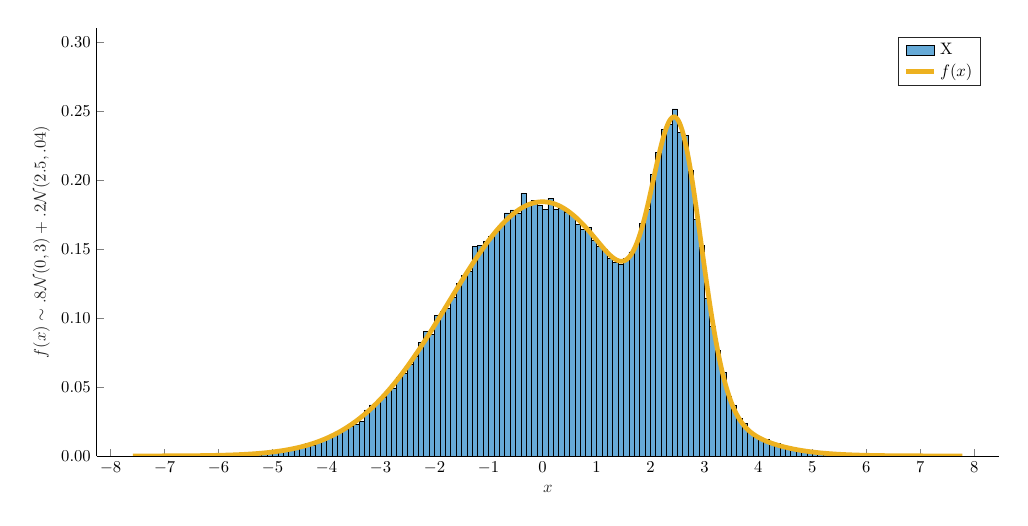
\begin{tikzpicture}[scale = 0.6]

\begin{axis}[%
width=7.521in,
height=3.566in,
at={(-0.1in,0.0in)},
scale only axis,
xmin=-8.26,
xmax=8.46,
xlabel style={font=\color{white!15!black}},
xlabel={$x$},
ymin=0,
ymax=0.31,
ylabel style={font=\color{white!15!black}},
ylabel={$f(x) \sim .8\mathcal{N}(0,3) +.2\mathcal{N}(2.5,.04)$},
y tick label style={
	/pgf/number format/.cd,
	fixed,
	fixed zerofill,
	precision=2,
	/tikz/.cd
},
axis background/.style={fill=white},
axis x line*=bottom,
axis y line*=left,
legend style={legend cell align=left, align=left, draw=white!15!black}
]
\addplot[ybar interval, fill=mycolor1, fill opacity=0.6, draw=black, area legend] table[row sep=crcr] {%
x	y\\
-7.5	0.0001\\
-7.4	9.99999999999995e-05\\
-7.3	0\\
-7.2	0\\
-7.1	0\\
-7	0\\
-6.9	0\\
-6.8	0.0001\\
-6.7	9.99999999999995e-05\\
-6.6	0\\
-6.5	0\\
-6.4	0\\
-6.3	0.000200000000000001\\
-6.2	0.000399999999999998\\
-6.1	0.000500000000000002\\
-6	0.000400000000000001\\
-5.9	0.000799999999999996\\
-5.8	0.000800000000000003\\
-5.7	0.00109999999999999\\
-5.6	0.000800000000000003\\
-5.5	0.00150000000000001\\
-5.4	0.00179999999999999\\
-5.3	0.00169999999999999\\
-5.2	0.00170000000000001\\
-5.1	0.00270000000000001\\
-5	0.00290000000000001\\
-4.9	0.00419999999999998\\
-4.8	0.00449999999999998\\
-4.7	0.00560000000000002\\
-4.6	0.00610000000000002\\
-4.5	0.00600000000000002\\
-4.4	0.00909999999999995\\
-4.3	0.00789999999999996\\
-4.2	0.0103\\
-4.1	0.0127\\
-4	0.0141\\
-3.9	0.0151\\
-3.8	0.0176\\
-3.7	0.0192\\
-3.6	0.0215000000000001\\
-3.5	0.0225999999999999\\
-3.4	0.0252000000000001\\
-3.3	0.0333000000000001\\
-3.2	0.0369999999999998\\
-3.1	0.0389000000000001\\
-3	0.0421999999999998\\
-2.9	0.0477000000000002\\
-2.8	0.0492999999999997\\
-2.7	0.0568000000000002\\
-2.6	0.0597000000000002\\
-2.5	0.0659999999999996\\
-2.4	0.0722000000000003\\
-2.3	0.0821999999999996\\
-2.2	0.0904000000000003\\
-2.1	0.0879000000000003\\
-2	0.101599999999999\\
-1.9	0.1044\\
-1.8	0.107099999999999\\
-1.7	0.1146\\
-1.6	0.1247\\
-1.5	0.130799999999999\\
-1.4	0.1339\\
-1.3	0.151599999999999\\
-1.2	0.152800000000001\\
-1.1	0.155400000000001\\
-1	0.159199999999999\\
-0.899999999999999	0.162600000000001\\
-0.8	0.167299999999999\\
-0.699999999999999	0.176000000000001\\
-0.6	0.178200000000001\\
-0.5	0.175899999999999\\
-0.399999999999999	0.190200000000001\\
-0.3	0.183299999999999\\
-0.199999999999999	0.184800000000001\\
-0.0999999999999996	0.181500000000001\\
0	0.178399999999999\\
0.100000000000001	0.186600000000001\\
0.2	0.178599999999999\\
0.300000000000001	0.179600000000001\\
0.4	0.176500000000001\\
0.5	0.174600000000001\\
0.6	0.167599999999998\\
0.700000000000001	0.164200000000001\\
0.800000000000001	0.165400000000001\\
0.9	0.155900000000001\\
1	0.151500000000001\\
1.1	0.149799999999998\\
1.2	0.143100000000001\\
1.3	0.140300000000001\\
1.4	0.1385\\
1.5	0.142800000000001\\
1.6	0.147799999999998\\
1.7	0.153500000000001\\
1.8	0.168300000000001\\
1.9	0.178700000000001\\
2	0.203699999999997\\
2.1	0.219800000000001\\
2.2	0.236400000000001\\
2.3	0.240100000000001\\
2.4	0.251400000000001\\
2.5	0.234099999999997\\
2.6	0.232300000000001\\
2.7	0.206800000000001\\
2.8	0.171300000000001\\
2.9	0.152700000000001\\
3	0.114199999999998\\
3.1	0.0937000000000003\\
3.2	0.0766000000000003\\
3.3	0.0602000000000002\\
3.4	0.0432000000000002\\
3.5	0.0364999999999995\\
3.6	0.0270000000000001\\
3.7	0.0237000000000001\\
3.8	0.0173000000000001\\
3.9	0.0134\\
4	0.0119999999999998\\
4.1	0.0119\\
4.2	0.0101\\
4.3	0.00910000000000003\\
4.4	0.00770000000000003\\
4.5	0.00559999999999992\\
4.6	0.00510000000000002\\
4.7	0.00400000000000001\\
4.8	0.00330000000000001\\
4.9	0.00370000000000001\\
5	0.00249999999999996\\
5.1	0.00180000000000001\\
5.2	0.0014\\
5.3	0.000500000000000002\\
5.4	0.000600000000000002\\
5.5	0.000799999999999989\\
5.6	0.000500000000000002\\
5.7	0.000800000000000003\\
5.8	0.000400000000000001\\
5.9	0.000900000000000003\\
6	0.00069999999999999\\
6.1	0.0001\\
6.2	0.0001\\
6.3	0.000500000000000002\\
6.4	0\\
6.5	0\\
6.6	0.0001\\
6.7	0.0001\\
6.8	0.0001\\
6.9	0.000200000000000001\\
7	0.000199999999999997\\
7.1	0\\
7.2	0\\
7.3	0.0001\\
7.4	0\\
7.5	0\\
7.6	0.0001\\
7.7	0.0001\\
};
\addlegendentry{X}

\addplot [color=mycolor3,line width = 1 mm]
  table[row sep=crcr]{%
-7.58847527370253	1.25011003560986e-05\\
-7.57309059475165	1.29966630944284e-05\\
-7.55770591580077	1.35108047056012e-05\\
-7.54232123684989	1.40441774317338e-05\\
-7.52693655789901	1.45974546491313e-05\\
-7.51155187894813	1.5171331485928e-05\\
-7.49616719999726	1.57665254553367e-05\\
-7.48078252104638	1.63837771048156e-05\\
-7.4653978420955	1.70238506814665e-05\\
-7.45001316314462	1.76875348139781e-05\\
-7.43462848419374	1.83756432114344e-05\\
-7.41924380524286	1.90890153793095e-05\\
-7.40385912629198	1.98285173529731e-05\\
-7.3884744473411	2.0595042449034e-05\\
-7.37308976839022	2.13895120348522e-05\\
-7.35770508943934	2.22128763165513e-05\\
-7.34232041048846	2.30661151458666e-05\\
-7.32693573153758	2.39502388461669e-05\\
-7.31155105258671	2.48662890579875e-05\\
-7.29616637363583	2.58153396044189e-05\\
-7.28078169468495	2.67984973766925e-05\\
-7.26539701573407	2.78169032403093e-05\\
-7.25001233678319	2.88717329620594e-05\\
-7.23462765783231	2.99641981582795e-05\\
-7.21924297888143	3.10955472646987e-05\\
-7.20385829993055	3.22670665282236e-05\\
-7.18847362097967	3.3480081021015e-05\\
-7.17308894202879	3.47359556772078e-05\\
-7.15770426307791	3.60360963526267e-05\\
-7.14231958412703	3.73819509078551e-05\\
-7.12693490517616	3.87750103150043e-05\\
-7.11155022622528	4.02168097885435e-05\\
-7.0961655472744	4.17089299405381e-05\\
-7.08078086832352	4.32529979606541e-05\\
-7.06539618937264	4.48506888212742e-05\\
-7.05001151042176	4.65037265080849e-05\\
-7.03462683147088	4.82138852764751e-05\\
-7.01924215252	4.99829909341009e-05\\
-7.00385747356912	5.1812922149959e-05\\
-6.98847279461824	5.37056117903158e-05\\
-6.97308811566736	5.56630482818274e-05\\
-6.95770343671648	5.76872770021989e-05\\
-6.94231875776561	5.97804016987081e-05\\
-6.92693407881473	6.19445859349335e-05\\
-6.91154939986385	6.41820545660112e-05\\
-6.89616472091297	6.64950952427458e-05\\
-6.88078004196209	6.8886059944895e-05\\
-6.86539536301121	7.13573665439433e-05\\
-6.85001068406033	7.39115003956743e-05\\
-6.83462600510945	7.65510159628445e-05\\
-6.81924132615857	7.92785384682595e-05\\
-6.80385664720769	8.20967655785416e-05\\
-6.78847196825681	8.50084691188744e-05\\
-6.77308728930594	8.8016496819004e-05\\
-6.75770261035506	9.11237740907631e-05\\
-6.74231793140418	9.43333058373843e-05\\
-6.7269332524533	9.76481782948505e-05\\
-6.71154857350242	0.000101071560905533\\
-6.69616389455154	0.000104606708224347\\
-6.68077921560066	0.000108256961857648\\
-6.66539453664978	0.000112025752435091\\
-6.6500098576989	0.00011591660161465\\
-6.63462517874802	0.000119933124120983\\
-6.61924049979714	0.000124079029817339\\
-6.60385582084626	0.000128358125811156\\
-6.58847114189539	0.000132774318593517\\
-6.57308646294451	0.000137331616212598\\
-6.55770178399363	0.000142034130481228\\
-6.54231710504275	0.000146886079218691\\
-6.52693242609187	0.000151891788526844\\
-6.51154774714099	0.000157055695100641\\
-6.49616306819011	0.000162382348573129\\
-6.48077838923923	0.000167876413894955\\
-6.46539371028835	0.000173542673748416\\
-6.45000903133747	0.000179386030996055\\
-6.43462435238659	0.000185411511163809\\
-6.41923967343572	0.000191624264958663\\
-6.40385499448484	0.000198029570820764\\
-6.38847031553396	0.000204632837509935\\
-6.37308563658308	0.000211439606726481\\
-6.3577009576322	0.000218455555766188\\
-6.34231627868132	0.000225686500209363\\
-6.32693159973044	0.000233138396643765\\
-6.31154692077956	0.000240817345421232\\
-6.29616224182868	0.0002487295934478\\
-6.2807775628778	0.000256881537007079\\
-6.26539288392692	0.000265279724616607\\
-6.25000820497604	0.000273930859916919\\
-6.23462352602517	0.000282841804592987\\
-6.21923884707429	0.000292019581327695\\
-6.20385416812341	0.000301471376786981\\
-6.18846948917253	0.00031120454463622\\
-6.17308481022165	0.000321226608587434\\
-6.15770013127077	0.000331545265476848\\
-6.14231545231989	0.00034216838837228\\
-6.12693077336901	0.000353104029709868\\
-6.11154609441813	0.000364360424459527\\
-6.09616141546725	0.000375945993318557\\
-6.08077673651637	0.000387869345932766\\
-6.06539205756549	0.000400139284144422\\
-6.05000737861462	0.000412764805266346\\
-6.03462269966374	0.000425755105381381\\
-6.01923802071286	0.000439119582666465\\
-6.00385334176198	0.000452867840740482\\
-5.9884686628111	0.000467009692035036\\
-5.97308398386022	0.000481555161187229\\
-5.95769930490934	0.000496514488453539\\
-5.94231462595846	0.000511898133143758\\
-5.92692994700758	0.000527716777074026\\
-5.9115452680567	0.000543981328037849\\
-5.89616058910582	0.000560702923294014\\
-5.88077591015495	0.000577892933070231\\
-5.86539123120407	0.000595562964081328\\
-5.85000655225319	0.000613724863060713\\
-5.83462187330231	0.000632390720303867\\
-5.81923719435143	0.000651572873222481\\
-5.80385251540055	0.000671283909907893\\
-5.78846783644967	0.000691536672702365\\
-5.77308315749879	0.000712344261776756\\
-5.75769847854791	0.000733720038713027\\
-5.74231379959703	0.000755677630090039\\
-5.72692912064615	0.000778230931070983\\
-5.71154444169527	0.000801394108990814\\
-5.6961597627444	0.000825181606941906\\
-5.68077508379352	0.000849608147356228\\
-5.66539040484264	0.000874688735582134\\
-5.65000572589176	0.000900438663453953\\
-5.63462104694088	0.000926873512852432\\
-5.61923636799	0.000954009159254027\\
-5.60385168903912	0.000981861775267046\\
-5.58846701008824	0.00101044783415255\\
-5.57308233113736	0.00103978411332784\\
-5.55769765218648	0.00106988769785043\\
-5.5423129732356	0.0011007759838801\\
-5.52692829428472	0.00113246668211695\\
-5.51154361533385	0.00116497782121291\\
-5.49615893638297	0.00119832775115442\\
-5.48077425743209	0.00123253514661379\\
-5.46538957848121	0.00126761901026671\\
-5.45000489953033	0.00130359867607338\\
-5.43462022057945	0.00134049381252069\\
-5.41923554162857	0.00137832442582264\\
-5.40385086267769	0.00141711086307641\\
-5.38846618372681	0.00145687381537131\\
-5.37308150477593	0.00149763432084771\\
-5.35769682582505	0.00153941376770309\\
-5.34231214687417	0.00158223389714237\\
-5.3269274679233	0.00162611680626942\\
-5.31154278897242	0.00167108495091682\\
-5.29615811002154	0.00171716114841074\\
-5.28077343107066	0.00176436858026783\\
-5.26538875211978	0.001812730794821\\
-5.2500040731689	0.00186227170977071\\
-5.23461939421802	0.0019130156146587\\
-5.21923471526714	0.00196498717326071\\
-5.20385003631626	0.00201821142589489\\
-5.18846535736538	0.00207271379164245\\
-5.1730806784145	0.00212852007047715\\
-5.15769599946363	0.00218565644530009\\
-5.14231132051275	0.00224414948387631\\
-5.12692664156187	0.00230402614066963\\
-5.11154196261099	0.00236531375857206\\
-5.09615728366011	0.00242804007052416\\
-5.08077260470923	0.00249223320102272\\
-5.06538792575835	0.00255792166751195\\
-5.05000324680747	0.0026251343816545\\
-5.03461856785659	0.0026939006504784\\
-5.01923388890571	0.00276425017739632\\
-5.00384920995483	0.00283621306309306\\
-4.98846453100395	0.00290981980627757\\
-4.97307985205308	0.00298510130429551\\
-4.9576951731022	0.00306208885359846\\
-4.94231049415132	0.00314081415006582\\
-4.92692581520044	0.00322130928917548\\
-4.91154113624956	0.00330360676601917\\
-4.89615645729868	0.00338773947515868\\
-4.8807717783478	0.00347374071031867\\
-4.86538709939692	0.0035616441639123\\
-4.85000242044604	0.00365148392639553\\
-4.83461774149516	0.00374329448544605\\
-4.81923306254428	0.0038371107249628\\
-4.8038483835934	0.00393296792388203\\
-4.78846370464253	0.00403090175480596\\
-4.77307902569165	0.00413094828243981\\
-4.75769434674077	0.00423314396183331\\
-4.74230966778989	0.00433752563642256\\
-4.72692498883901	0.00444413053586839\\
-4.71154030988813	0.00455299627368703\\
-4.69615563093725	0.00466416084466918\\
-4.68077095198637	0.00477766262208356\\
-4.66538627303549	0.00489354035466095\\
-4.65000159408461	0.00501183316335481\\
-4.63461691513373	0.00513258053787461\\
-4.61923223618285	0.00525582233298801\\
-4.60384755723198	0.00538159876458807\\
-4.5884628782811	0.00550995040552174\\
-4.57307819933022	0.00564091818117585\\
-4.55769352037934	0.00577454336481692\\
-4.54230884142846	0.00591086757268124\\
-4.52692416247758	0.00604993275881147\\
-4.5115394835267	0.00619178120963643\\
-4.49615480457582	0.00633645553829034\\
-4.48077012562494	0.00648399867866845\\
-4.46538544667406	0.00663445387921545\\
-4.45000076772318	0.00678786469644343\\
-4.43461608877231	0.00694427498817639\\
-4.41923140982143	0.00710372890651788\\
-4.40384673087055	0.00726627089053909\\
-4.38846205191967	0.0074319456586841\\
-4.37307737296879	0.00760079820088962\\
-4.35769269401791	0.00777287377041657\\
-4.34230801506703	0.00794821787539057\\
-4.32692333611615	0.00812687627004893\\
-4.31153865716527	0.0083088949456917\\
-4.29615397821439	0.00849432012133438\\
-4.28076929926351	0.00868319823406015\\
-4.26538462031263	0.00887557592906926\\
-4.24999994136176	0.00907150004942399\\
-4.23461526241088	0.00927101762548697\\
-4.21923058346	0.00947417586405122\\
-4.20384590450912	0.00968102213716037\\
-4.18846122555824	0.00989160397061754\\
-4.17307654660736	0.0101059690321817\\
-4.15769186765648	0.0103241651194499\\
-4.1423071887056	0.010546240147425\\
-4.12692250975472	0.0107722421357673\\
-4.11153783080384	0.0110022191957305\\
-4.09615315185297	0.0112362195167791\\
-4.08076847290208	0.0114742913528903\\
-4.06538379395121	0.011716483008537\\
-4.04999911500033	0.0119628428243535\\
-4.03461443604945	0.0122134191624838\\
-4.01922975709857	0.0124682603916124\\
-4.00384507814769	0.0127274148716785\\
-3.98846039919681	0.0129909309382744\\
-3.97307572024593	0.013258856886728\\
-3.95769104129505	0.0135312409558719\\
-3.94230636234417	0.0138081313114992\\
-3.92692168339329	0.014089576029508\\
-3.91153700444241	0.014375623078736\\
-3.89615232549153	0.0146663203034875\\
-3.88076764654066	0.0149617154057544\\
-3.86538296758978	0.0152618559271336\\
-3.8499982886389	0.0155667892304434\\
-3.83461360968802	0.015876562481042\\
-3.81922893073714	0.0161912226278502\\
-3.80384425178626	0.0165108163840818\\
-3.78845957283538	0.0168353902076863\\
-3.7730748938845	0.0171649902815046\\
-3.75769021493362	0.0174996624931456\\
-3.74230553598274	0.0178394524145837\\
-3.72692085703186	0.0181844052814845\\
-3.71153617808099	0.0185345659722622\\
-3.69615149913011	0.0188899789868726\\
-3.68076682017923	0.0192506884253489\\
-3.66538214122835	0.0196167379660831\\
-3.64999746227747	0.0199881708438605\\
-3.63461278332659	0.0203650298276521\\
-3.61922810437571	0.0207473571981712\\
-3.60384342542483	0.0211351947251998\\
-3.58845874647395	0.021528583644693\\
-3.57307406752307	0.0219275646356655\\
-3.55768938857219	0.0223321777968705\\
-3.54230470962132	0.0227424626232748\\
-3.52692003067044	0.0231584579823402\\
-3.51153535171956	0.0235802020901179\\
-3.49615067276868	0.0240077324871638\\
-3.4807659938178	0.024441086014283\\
-3.46538131486692	0.0248802987881125\\
-3.44999663591604	0.02532540617655\\
-3.43461195696516	0.0257764427740384\\
-3.41922727801428	0.0262334423767148\\
-3.4038425990634	0.0266964379574341\\
-3.38845792011252	0.0271654616406753\\
-3.37307324116164	0.0276405446773433\\
-3.35768856221076	0.0281217174194727\\
-3.34230388325989	0.0286090092948472\\
-3.32691920430901	0.0291024487815436\\
-3.31153452535813	0.0296020633824107\\
-3.29614984640725	0.0301078795994969\\
-3.28076516745637	0.0306199229084333\\
-3.26538048850549	0.0311382177327892\\
-3.24999580955461	0.0316627874184068\\
-3.23461113060373	0.0321936542077302\\
-3.21922645165285	0.0327308392141398\\
-3.20384177270197	0.0332743623963036\\
-3.18845709375109	0.0338242425325603\\
-3.17307241480022	0.0343804971953442\\
-3.15768773584934	0.0349431427256661\\
-3.14230305689846	0.0355121942076644\\
-3.12691837794758	0.0360876654432367\\
-3.1115336989967	0.0366695689267692\\
-3.09614902004582	0.0372579158199738\\
-3.08076434109494	0.0378527159268493\\
-3.06537966214406	0.03845397766878\\
-3.04999498319318	0.039061708059784\\
-3.0346103042423	0.0396759126819289\\
-3.01922562529142	0.0402965956609259\\
-3.00384094634054	0.0409237596419186\\
-2.98845626738967	0.0415574057654807\\
-2.97307158843879	0.0421975336438371\\
-2.95768690948791	0.0428441413373237\\
-2.94230223053703	0.0434972253311003\\
-2.92691755158615	0.0441567805121321\\
-2.91153287263527	0.0448228001464539\\
-2.89614819368439	0.045495275856734\\
-2.88076351473351	0.0461741976001509\\
-2.86537883578263	0.0468595536465999\\
-2.84999415683175	0.0475513305572435\\
-2.83460947788087	0.048249513163422\\
-2.81922479893	0.0489540845459389\\
-2.80384011997912	0.0496650260147376\\
-2.78845544102824	0.0503823170889835\\
-2.77307076207736	0.0511059354775676\\
-2.75768608312648	0.0518358570600476\\
-2.7423014041756	0.05257205586804\\
-2.72691672522472	0.0533145040670818\\
-2.71153204627384	0.0540631719389729\\
-2.69614736732296	0.0548180278646189\\
-2.68076268837208	0.0555790383073854\\
-2.6653780094212	0.0563461677969823\\
-2.64999333047032	0.0571193789138915\\
-2.63460865151945	0.0578986322743525\\
-2.61922397256857	0.0586838865159224\\
-2.60383929361769	0.0594750982836235\\
-2.58845461466681	0.0602722222166943\\
-2.57306993571593	0.0610752109359574\\
-2.55768525676505	0.0618840150318194\\
-2.54230057781417	0.0626985830529166\\
-2.52691589886329	0.0635188614954207\\
-2.51153121991241	0.0643447947930178\\
-2.49614654096153	0.0651763253075756\\
-2.48076186201065	0.0660133933205105\\
-2.46537718305978	0.0668559370248698\\
-2.4499925041089	0.0677038925181397\\
-2.43460782515802	0.0685571937957939\\
-2.41922314620714	0.0694157727455949\\
-2.40383846725626	0.0702795591426588\\
-2.38845378830538	0.0711484806452973\\
-2.3730691093545	0.0720224627916482\\
-2.35768443040362	0.0729014289971048\\
-2.34229975145274	0.0737853005525573\\
-2.32691507250186	0.0746739966234542\\
-2.31153039355098	0.0755674342496975\\
-2.2961457146001	0.0764655283463787\\
-2.28076103564922	0.0773681917053673\\
-2.26537635669835	0.0782753349977613\\
-2.24999167774747	0.0791868667772073\\
-2.23460699879659	0.0801026934841\\
-2.21922231984571	0.0810227194506702\\
-2.20383764089483	0.0819468469069662\\
-2.18845296194395	0.0828749759877406\\
-2.17306828299307	0.0838070047402451\\
-2.15768360404219	0.0847428291329429\\
-2.14229892509131	0.0856823430651442\\
-2.12691424614043	0.0866254383775695\\
-2.11152956718955	0.0875720048638482\\
-2.09614488823868	0.0885219302829551\\
-2.0807602092878	0.089475100372591\\
-2.06537553033692	0.0904313988635098\\
-2.04999085138604	0.0913907074947973\\
-2.03460617243516	0.0923529060301028\\
-2.01922149348428	0.0933178722748276\\
-2.0038368145334	0.0942854820942716\\
-1.98845213558252	0.0952556094327386\\
-1.97306745663164	0.0962281263336034\\
-1.95768277768076	0.0972029029603391\\
-1.94229809872988	0.0981798076185056\\
-1.92691341977901	0.0991587067786974\\
-1.91152874082813	0.100139465100452\\
-1.89614406187725	0.101121945457115\\
-1.88075938292637	0.102106008961657\\
-1.86537470397549	0.10309151499345\\
-1.84999002502461	0.104078321225985\\
-1.83460534607373	0.105066283655535\\
-1.81922066712285	0.106055256630769\\
-1.80383598817197	0.107045092883282\\
-1.78845130922109	0.108035643559076\\
-1.77306663027021	0.109026758250945\\
-1.75768195131933	0.110018285031791\\
-1.74229727236845	0.11101007048884\\
-1.72691259341758	0.112001959758766\\
-1.7115279144667	0.112993796563702\\
-1.69614323551582	0.113985423248137\\
-1.68075855656494	0.114976680816689\\
-1.66537387761406	0.115967408972739\\
-1.64998919866318	0.116957446157921\\
-1.6346045197123	0.117946629592445\\
-1.61921984076142	0.118934795316267\\
-1.60383516181054	0.119921778231057\\
-1.58845048285966	0.120907412142984\\
-1.57306580390878	0.121891529806284\\
-1.55768112495791	0.122873962967615\\
-1.54229644600703	0.12385454241116\\
-1.52691176705615	0.124833098004486\\
-1.51152708810527	0.125809458745132\\
-1.49614240915439	0.126783452807908\\
-1.48075773020351	0.127754907592897\\
-1.46537305125263	0.128723649774135\\
-1.44998837230175	0.129689505348949\\
-1.43460369335087	0.130652299687948\\
-1.41921901439999	0.131611857585629\\
-1.40383433544911	0.132568003311598\\
-1.38844965649823	0.133520560662372\\
-1.37306497754736	0.134469353013747\\
-1.35768029859648	0.135414203373712\\
-1.3422956196456	0.136354934435885\\
-1.32691094069472	0.137291368633456\\
-1.31152626174384	0.138223328193601\\
-1.29614158279296	0.139150635192363\\
-1.28075690384208	0.140073111609962\\
-1.2653722248912	0.140990579386514\\
-1.24998754594032	0.141902860478148\\
-1.23460286698944	0.142809776913471\\
-1.21921818803856	0.143711150850385\\
-1.20383350908768	0.144606804633215\\
-1.18844883013681	0.145496560850119\\
-1.17306415118593	0.14638024239077\\
-1.15767947223505	0.147257672504273\\
-1.14229479328417	0.148128674857295\\
-1.12691011433329	0.148993073592374\\
-1.11152543538241	0.1498506933864\\
-1.09614075643153	0.150701359509213\\
-1.08075607748065	0.151544897882318\\
-1.06537139852977	0.152381135137671\\
-1.04998671957889	0.153209898676519\\
-1.03460204062801	0.15403101672826\\
-1.01921736167714	0.154844318409301\\
-1.00383268272626	0.155649633781878\\
-0.988448003775377	0.156446793912821\\
-0.973063324824498	0.157235630932226\\
-0.957678645873619	0.158015978092008\\
-0.942293966922739	0.158787669824314\\
-0.926909287971861	0.159550541799752\\
-0.911524609020982	0.160304430985425\\
-0.896139930070102	0.161049175702733\\
-0.880755251119223	0.161784615684907\\
-0.865370572168344	0.162510592134267\\
-0.849985893217465	0.16322694777915\\
-0.834601214266586	0.163933526930502\\
-0.819216535315706	0.164630175538091\\
-0.803831856364827	0.16531674124632\\
-0.788447177413948	0.165993073449607\\
-0.773062498463069	0.166659023347312\\
-0.757677819512191	0.167314443998169\\
-0.74229314056131	0.167959190374212\\
-0.726908461610432	0.168593119414153\\
-0.711523782659553	0.169216090076195\\
-0.696139103708673	0.169827963390244\\
-0.680754424757795	0.170428602509502\\
-0.665369745806915	0.171017872761409\\
-0.649985066856035	0.171595641697902\\
-0.634600387905157	0.172161779144981\\
-0.619215708954278	0.172716157251539\\
-0.603831030003399	0.173258650537437\\
-0.588446351052519	0.173789135940809\\
-0.57306167210164	0.17430749286455\\
-0.557676993150761	0.174813603221984\\
-0.542292314199882	0.175307351481676\\
-0.526907635249003	0.175788624711367\\
-0.511522956298124	0.176257312621016\\
-0.496138277347244	0.176713307604906\\
-0.480753598396365	0.177156504782823\\
-0.465368919445487	0.177586802040259\\
-0.449984240494607	0.178004100067626\\
-0.434599561543727	0.178408302398475\\
-0.419214882592849	0.178799315446676\\
-0.403830203641969	0.179177048542559\\
-0.388445524691091	0.17954141396799\\
-0.373060845740212	0.179892326990365\\
-0.357676166789332	0.180229705895507\\
-0.342291487838453	0.180553472019449\\
-0.326906808887574	0.180863549779086\\
-0.311522129936695	0.181159866701691\\
-0.296137450985816	0.181442353453274\\
-0.280752772034936	0.181710943865773\\
-0.265368093084057	0.181965574963073\\
-0.249983414133178	0.182206186985844\\
-0.234598735182299	0.182432723415183\\
-0.21921405623142	0.182645130995072\\
-0.20382937728054	0.182843359753631\\
-0.188444698329661	0.183027363023183\\
-0.173060019378783	0.183197097459119\\
-0.157675340427904	0.183352523057588\\
-0.142290661477024	0.183493603171997\\
-0.126905982526145	0.183620304528361\\
-0.111521303575266	0.1837325972395\\
-0.0961366246243864	0.183830454818116\\
-0.0807519456735077	0.183913854188779\\
-0.065367266722629	0.183982775698856\\
-0.0499825877717486	0.184037203128418\\
-0.0345979088208699	0.184077123699195\\
-0.0192132298699912	0.184102528082615\\
-0.00382855091911249	0.184113410407015\\
0.0115561280317671	0.184109768264102\\
0.0269408069826467	0.184091602714755\\
0.0423254859335254	0.184058918294289\\
0.0577101648844049	0.184011723017296\\
0.0730948438352836	0.183950028382226\\
0.0884795227861623	0.183873849375864\\
0.103864201737043	0.183783204477903\\
0.119248880687921	0.183678115665827\\
0.1346335596388	0.183558608420366\\
0.15001823858968	0.183424711731791\\
0.165402917540558	0.183276458107383\\
0.180787596491438	0.183113883580429\\
0.196172275442317	0.18293702772116\\
0.211556954393196	0.182745933650088\\
0.226941633344075	0.182540648054252\\
0.242326312294954	0.182321221206956\\
0.257710991245834	0.182087706991637\\
0.273095670196713	0.181840162930583\\
0.288480349147592	0.181578650219297\\
0.303865028098471	0.181303233767387\\
0.31924970704935	0.181013982246968\\
0.334634386000229	0.180710968149652\\
0.350019064951109	0.180394267853319\\
0.365403743901988	0.180063961699971\\
0.380788422852866	0.179720134086119\\
0.396173101803745	0.179362873567254\\
0.411557780754626	0.178992272978128\\
0.426942459705504	0.1786084295707\\
0.442327138656383	0.178211445171771\\
0.457711817607262	0.177801426362497\\
0.473096496558142	0.177378484682123\\
0.488481175509021	0.176942736858499\\
0.5038658544599	0.176494305068075\\
0.519250533410778	0.176033317228283\\
0.534635212361659	0.175559907325409\\
0.550019891312537	0.175074215781223\\
0.565404570263416	0.174576389861829\\
0.580789249214297	0.174066584132397\\
0.596173928165175	0.173544960961581\\
0.611558607116054	0.173011691079603\\
0.626943286066933	0.172466954194156\\
0.642327965017811	0.171910939668354\\
0.65771264396869	0.171343847265124\\
0.673097322919569	0.170765887962482\\
0.688482001870451	0.170177284844176\\
0.70386668082133	0.169578274070225\\
0.719251359772208	0.168969105931811\\
0.734636038723087	0.168350045994909\\
0.750020717673966	0.167721376336914\\
0.765405396624844	0.167083396880297\\
0.780790075575725	0.166436426827044\\
0.796174754526604	0.165780806197299\\
0.811559433477482	0.165116897475178\\
0.826944112428361	0.164445087364169\\
0.842328791379241	0.163765788653941\\
0.85771347033012	0.1630794421996\\
0.873098149281001	0.162386519013613\\
0.888482828231879	0.161687522469614\\
0.903867507182758	0.160982990616231\\
0.919252186133637	0.160273498597835\\
0.934636865084515	0.159559661177754\\
0.950021544035394	0.158842135357978\\
0.965406222986273	0.158121623087791\\
0.980790901937153	0.15739887405195\\
0.996175580888034	0.156674688527155\\
1.01156025983891	0.155949920293525\\
1.02694493878979	0.155225479585625\\
1.04232961774067	0.154502336065345\\
1.05771429669155	0.153781521796551\\
1.07309897564243	0.153064134198978\\
1.08848365459331	0.152351338956311\\
1.10386833354419	0.151644372850836\\
1.11925301249507	0.150944546494421\\
1.13463769144594	0.150253246923021\\
1.15002237039682	0.149571940019276\\
1.1654070493477	0.148902172725324\\
1.18079172829858	0.148245575005469\\
1.19617640724946	0.147603861516115\\
1.21156108620034	0.146978832938224\\
1.22694576515122	0.146372376925697\\
1.2423304441021	0.145786468621415\\
1.25771512305298	0.145223170691376\\
1.27309980200386	0.144684632826372\\
1.28848448095474	0.144173090660095\\
1.30386915990562	0.143690864052423\\
1.3192538388565	0.143240354687041\\
1.33463851780737	0.142824042933434\\
1.35002319675825	0.142444483924819\\
1.36540787570913	0.142104302805705\\
1.38079255466001	0.141806189105555\\
1.39617723361089	0.141552890198505\\
1.41156191256177	0.14134720381333\\
1.42694659151265	0.141191969562742\\
1.44233127046353	0.141090059466853\\
1.45771594941441	0.141044367452062\\
1.47310062836529	0.141057797813837\\
1.48848530731617	0.141133252639811\\
1.50386998626704	0.141273618198285\\
1.51925466521792	0.141481750306527\\
1.5346393441688	0.141760458703278\\
1.55002402311968	0.142112490460371\\
1.56540870207056	0.142540512479441\\
1.58079338102144	0.143047093131158\\
1.59617805997232	0.143634683106203\\
1.6115627389232	0.144305595559224\\
1.62694741787408	0.145061985639139\\
1.64233209682496	0.14590582951122\\
1.65771677577584	0.146838902988384\\
1.67310145472671	0.147862759900724\\
1.68848613367759	0.148978710343533\\
1.70387081262847	0.15018779895469\\
1.71925549157935	0.151490783382098\\
1.73464017053023	0.152888113110799\\
1.75002484948111	0.154379908827265\\
1.76540952843199	0.155965942504968\\
1.78079420738287	0.157645618400577\\
1.79617888633375	0.159417955153866\\
1.81156356528463	0.161281569186478\\
1.82694824423551	0.163234659594976\\
1.84233292318638	0.165274994732014\\
1.85771760213726	0.167399900665917\\
1.87310228108814	0.169606251703328\\
1.88848696003902	0.171890463151879\\
1.9038716389899	0.174248486490045\\
1.91925631794078	0.176675807099363\\
1.93464099689166	0.179167444700174\\
1.95002567584254	0.18171795661594\\
1.96541035479342	0.184321443973125\\
1.9807950337443	0.186971560923677\\
1.99617971269518	0.189661526955484\\
2.01156439164606	0.192384142332892\\
2.02694907059693	0.195131806684744\\
2.04233374954781	0.197896540731536\\
2.05771842849869	0.200670011116487\\
2.07310310744957	0.203443558277825\\
2.08848778640045	0.206208227271661\\
2.10387246535133	0.208954801426718\\
2.11925714430221	0.211673838684297\\
2.13464182325309	0.214355710449366\\
2.15002650220397	0.216990642751967\\
2.16541118115485	0.21956875949256\\
2.18079586010573	0.222080127520679\\
2.19618053905661	0.224514803273779\\
2.21156521800748	0.226862880682645\\
2.22694989695836	0.22911454003145\\
2.24233457590924	0.231260097444838\\
2.25771925486012	0.233290054661424\\
2.273103933811	0.235195148743056\\
2.28848861276188	0.23696640136232\\
2.30387329171276	0.238595167307136\\
2.31925797066364	0.240073181841028\\
2.33464264961452	0.241392606560897\\
2.3500273285654	0.242546073400727\\
2.36541200751627	0.243526726439832\\
2.38079668646716	0.244328261187741\\
2.39618136541804	0.244944961034625\\
2.41156604436891	0.245371730576193\\
2.42695072331979	0.245604125544902\\
2.44233540227067	0.245638379105098\\
2.45772008122155	0.245471424297968\\
2.47310476017243	0.245100912452656\\
2.48848943912331	0.244525227412363\\
2.50387411807419	0.243743495458259\\
2.51925879702507	0.242755590849314\\
2.53464347597595	0.241562136932291\\
2.55002815492683	0.240164502812764\\
2.5654128338777	0.238564795614756\\
2.58079751282859	0.23676584839301\\
2.59618219177946	0.234771203797661\\
2.61156687073034	0.232585093625756\\
2.62695154968122	0.23021241442736\\
2.6423362286321	0.227658699365461\\
2.65772090758298	0.224930086558322\\
2.67310558653386	0.222033284159931\\
2.68849026548474	0.218975532458589\\
2.70387494443562	0.21576456329516\\
2.7192596233865	0.212408557120912\\
2.73464430233738	0.208916098030045\\
2.75002898128825	0.205296127113839\\
2.76541366023913	0.201557894491711\\
2.78079833919001	0.197710910379402\\
2.79618301814089	0.193764895555991\\
2.81156769709177	0.18972973158943\\
2.82695237604265	0.185615411175068\\
2.84233705499353	0.181431988933094\\
2.85772173394441	0.177189532999322\\
2.87310641289529	0.172898077729318\\
2.88849109184617	0.168567577818879\\
2.90387577079705	0.164207864124385\\
2.91926044974793	0.159828601445045\\
2.9346451286988	0.155439248505609\\
2.95002980764968	0.151049020353204\\
2.96541448660056	0.146666853355733\\
2.98079916555144	0.142301372962175\\
2.99618384450232	0.137960864357378\\
3.0115685234532	0.133653246115908\\
3.02695320240408	0.129386046931456\\
3.04233788135496	0.125166385470583\\
3.05772256030584	0.121000953372375\\
3.07310723925672	0.116896001389239\\
3.0884919182076	0.112857328638813\\
3.10387659715848	0.108890274912966\\
3.11926127610935	0.104999715967384\\
3.13464595506023	0.101190061694422\\
3.15003063401111	0.0974652570628836\\
3.16541531296199	0.0938287856913041\\
3.18079999191287	0.0902836759062393\\
3.19618467086375	0.0868325091240831\\
3.21156934981463	0.083477430384039\\
3.22695402876551	0.0802201608511429\\
3.24233870771639	0.0770620121015749\\
3.25772338666727	0.0740039019979333\\
3.27310806561814	0.0710463719595837\\
3.28849274456902	0.0681896054325604\\
3.30387742351991	0.0654334473647015\\
3.31926210247078	0.0627774244946117\\
3.33464678142166	0.060220766267557\\
3.35003146037254	0.0577624261973568\\
3.36541613932342	0.055401103500596\\
3.3808008182743	0.0531352648379034\\
3.39618549722518	0.0509631660064506\\
3.41157017617606	0.0488828734380695\\
3.42695485512694	0.0468922853683216\\
3.44233953407782	0.044989152553287\\
3.4577242130287	0.0431710984226686\\
3.47310889197957	0.0414356385698433\\
3.48849357093045	0.0397801994916167\\
3.50387824988133	0.0382021365025275\\
3.51926292883221	0.036698750760452\\
3.53464760778309	0.0352673053519103\\
3.55003228673397	0.0339050403967307\\
3.56541696568485	0.032609187142535\\
3.58080164463573	0.0313769810297675\\
3.59618632358661	0.0302056737176473\\
3.61157100253749	0.0290925440704249\\
3.62695568148837	0.0280349081116319\\
3.64234036043925	0.0270301279615827\\
3.65772503939012	0.0260756197802244\\
3.673109718341	0.0251688607435018\\
3.68849439729188	0.0243073950867231\\
3.70387907624276	0.0234888392529854\\
3.71926375519364	0.0227108861885555\\
3.73464843414452	0.0219713088302395\\
3.7500331130954	0.0212679628322216\\
3.76541779204628	0.0205987885816692\\
3.78080247099716	0.0199618125535969\\
3.79618714994804	0.0193551480561301\\
3.81157182889892	0.0187769954174224\\
3.8269565078498	0.0182256416651325\\
3.84234118680067	0.0176994597485884\\
3.85772586575155	0.0171969073526079\\
3.87311054470243	0.0167165253504623\\
3.88849522365331	0.0162569359416982\\
3.90387990260419	0.0158168405185265\\
3.91926458155507	0.0153950173022826\\
3.93464926050595	0.014990318789112\\
3.95003393945683	0.0146016690415592\\
3.96541861840771	0.0142280608601985\\
3.98080329735859	0.0138685528668491\\
3.99618797630947	0.0135222665283163\\
4.01157265526034	0.0131883831470105\\
4.02695733421122	0.0128661408422437\\
4.0423420131621	0.012554831543515\\
4.05772669211298	0.0122537980146843\\
4.07311137106386	0.0119624309256153\\
4.08849605001474	0.0116801659856626\\
4.10388072896562	0.0114064811512826\\
4.1192654079165	0.0111408939180841\\
4.13465008686738	0.0108829587057988\\
4.15003476581826	0.0106322643429501\\
4.16541944476914	0.0103884316564363\\
4.18080412372002	0.010151111169813\\
4.19618880267089	0.00991998091276845\\
4.21157348162177	0.00969474434311861\\
4.22695816057265	0.00947512838161732\\
4.24234283952353	0.00926088155896077\\
4.25772751847441	0.00905177227357054\\
4.27311219742529	0.00884758715805227\\
4.28849687637617	0.00864812955164559\\
4.30388155532705	0.00845321807549381\\
4.31926623427793	0.00826268530716551\\
4.33465091322881	0.00807637655054534\\
4.35003559217968	0.00789414869697077\\
4.36542027113056	0.0077158691733188\\
4.38080495008144	0.00754141497263411\\
4.39618962903232	0.00737067176283139\\
4.4115743079832	0.00720353306899267\\
4.42695898693408	0.00703989952481011\\
4.44234366588496	0.00687967818878938\\
4.45772834483584	0.00672278192092281\\
4.47311302378672	0.00656912881566147\\
4.4884977027376	0.00641864168715468\\
4.50388238168848	0.00627124760288155\\
4.51926706063936	0.0061268774619669\\
4.53465173959023	0.00598546561465188\\
4.55003641854112	0.00584694951957183\\
4.56542109749199	0.00571126943568127\\
4.58080577644287	0.00557836814585237\\
4.59619045539375	0.00544819070936101\\
4.61157513434463	0.00532068424065686\\
4.62695981329551	0.00519579771199489\\
4.64234449224639	0.00507348177767936\\
4.65772917119727	0.00495368861783987\\
4.67311385014815	0.00483637179982033\\
4.68849852909903	0.00472148615541551\\
4.70388320804991	0.00460898767233596\\
4.71926788700079	0.0044988333984196\\
4.73465256595166	0.00439098135723839\\
4.75003724490254	0.00428539047386988\\
4.76542192385342	0.00418202050971637\\
4.7808066028043	0.00408083200536042\\
4.79619128175518	0.00398178623054245\\
4.81157596070606	0.00388484514043672\\
4.82696063965694	0.0037899713374847\\
4.84234531860782	0.00369712803812112\\
4.8577299975587	0.00360627904379738\\
4.87311467650958	0.0035173887157709\\
4.88849935546046	0.00343042195318626\\
4.90388403441134	0.00334534417402699\\
4.91926871336221	0.00326212129856378\\
4.93465339231309	0.00318071973496808\\
4.95003807126397	0.00310110636679842\\
4.96542275021485	0.00302324854210138\\
4.98080742916573	0.00294711406390032\\
4.99619210811661	0.00287267118187262\\
5.01157678706749	0.00279988858504072\\
5.02696146601837	0.00272873539532481\\
5.04234614496925	0.00265918116182376\\
5.05773082392013	0.00259119585570895\\
5.073115502871	0.00252474986563056\\
5.08850018182189	0.00245981399354927\\
5.10388486077276	0.00239635945091878\\
5.11926953972364	0.00233435785515407\\
5.13465421867452	0.00227378122633056\\
5.1500388976254	0.0022146019840664\\
5.16542357657628	0.00215679294454759\\
5.18080825552716	0.00210032731766171\\
5.19619293447804	0.00204517870421112\\
5.21157761342892	0.00199132109318119\\
5.2269622923798	0.00193872885904322\\
5.24234697133068	0.00188737675907489\\
5.25773165028155	0.00183723993068429\\
5.27311632923243	0.00178829388872591\\
5.28850100818331	0.00174051452279926\\
5.30388568713419	0.0016938780945228\\
5.31927036608507	0.00164836123477707\\
5.33465504503595	0.0016039409409127\\
5.35003972398683	0.0015605945739199\\
5.36542440293771	0.00151829985555697\\
5.38080908188859	0.00147703486543636\\
5.39619376083947	0.00143677803806748\\
5.41157843979035	0.00139750815985573\\
5.42696311874123	0.00135920436605831\\
5.4423477976921	0.00132184613769711\\
5.45773247664298	0.00128541329842985\\
5.47311715559386	0.00124988601138046\\
5.48850183454474	0.00121524477593035\\
5.50388651349562	0.00118147042447206\\
5.5192711924465	0.001148544119127\\
5.53465587139738	0.0011164473484292\\
5.55004055034826	0.00108516192397705\\
5.56542522929914	0.00105466997705491\\
5.58080990825002	0.00102495395522667\\
5.5961945872009	0.000995996618903365\\
5.61157926615178	0.000967781037886865\\
5.62696394510266	0.000940290587891716\\
5.64234862405353	0.000913508947047232\\
5.65773330300441	0.000887420092381835\\
5.67311798195529	0.000862008296291705\\
5.68850266090617	0.000837258122995731\\
5.70388733985705	0.000813154424978719\\
5.71927201880793	0.000789682339424782\\
5.73465669775881	0.000766827284642828\\
5.75004137670969	0.000744574956485983\\
5.76542605566057	0.000722911324766761\\
5.78081073461145	0.000701822629669733\\
5.79619541356233	0.000681295378163477\\
5.81158009251321	0.000661316340413372\\
5.82696477146408	0.000641872546196997\\
5.84234945041496	0.000622951281323637\\
5.85773412936584	0.000604540084059456\\
5.87311880831672	0.000586626741559837\\
5.8885034872676	0.000569199286310324\\
5.90388816621848	0.000552245992577587\\
5.91927284516936	0.000535755372871723\\
5.93465752412024	0.000519716174421251\\
5.95004220307112	0.000504117375662036\\
5.965426882022	0.000488948182741358\\
5.98081156097288	0.000474198026038315\\
5.99619623992375	0.000459856556701693\\
6.01158091887463	0.00044591364320636\\
6.02696559782551	0.000432359367929277\\
6.04235027677639	0.000419184023746082\\
6.05773495572727	0.000406378110649247\\
6.07311963467815	0.000393932332388696\\
6.08850431362903	0.000381837593135789\\
6.10388899257991	0.00037008499417151\\
6.11927367153079	0.000358665830599633\\
6.13465835048167	0.000347571588085675\\
6.15004302943255	0.000336793939622331\\
6.16542770838342	0.000326324742322089\\
6.1808123873343	0.000316156034237677\\
6.19619706628518	0.000306280031210973\\
6.21158174523606	0.000296689123750939\\
6.22696642418694	0.000287375873941148\\
6.24235110313782	0.000278333012377416\\
6.2577357820887	0.000269553435136017\\
6.27312046103958	0.000261030200772938\\
6.28850513999046	0.000252756527354595\\
6.30388981894134	0.000244725789520404\\
6.31927449789222	0.000236931515577556\\
6.3346591768431	0.000229367384628348\\
6.35004385579397	0.000222027223730352\\
6.36542853474485	0.00021490500508972\\
6.38081321369573	0.000207994843287853\\
6.39619789264661	0.000201290992541678\\
6.41158257159749	0.000194787843997719\\
6.42696725054837	0.000188479923060134\\
6.44235192949925	0.000182361886752877\\
6.45773660845013	0.000176428521116101\\
6.47312128740101	0.000170674738636919\\
6.48850596635189	0.000165095575714582\\
6.50389064530277	0.000159686190160161\\
6.51927532425364	0.000154441858730747\\
6.53466000320452	0.000149357974698209\\
6.5500446821554	0.000144430045452492\\
6.56542936110628	0.00013965369013946\\
6.58081404005716	0.000135024637333209\\
6.59619871900804	0.000130538722742843\\
6.61158339795892	0.000126191886953598\\
6.6269680769098	0.000121980173202258\\
6.64235275586068	0.000117899725186738\\
6.65773743481156	0.00011394678490973\\
6.67312211376244	0.00011011769055627\\
6.68850679271332	0.000106408874405085\\
6.7038914716642	0.000102816860773556\\
6.71927615061507	9.93382639961195e-05\\
6.73466082956595	9.59697864359359e-05\\
6.75004550851683	9.27082165296096e-05\\
6.76543018746771	8.95504268647656e-05\\
6.78081486641859	8.64933722902568e-05\\
6.79619954536947	8.35340880587739e-05\\
6.81158422432035	8.06696880016167e-05\\
6.82696890327123	7.78973627353815e-05\\
6.84235358222211	7.52143779003036e-05\\
6.85773826117299	7.26180724299898e-05\\
6.87312294012387	7.01058568522695e-05\\
6.88850761907475	6.76752116208774e-05\\
6.90389229802562	6.53236854776878e-05\\
6.9192769769765	6.30488938451946e-05\\
6.93466165592738	6.08485172489479e-05\\
6.95004633487826	5.87202997696296e-05\\
6.96543101382914	5.66620475244631e-05\\
6.98081569278002	5.46716271776359e-05\\
6.9962003717309	5.27469644794119e-05\\
7.01158505068178	5.08860428336135e-05\\
7.02696972963266	4.90869018931338e-05\\
7.04235440858354	4.73476361831536e-05\\
7.05773908753442	4.56663937517204e-05\\
7.07312376648529	4.40413748473519e-05\\
7.08850844543617	4.24708306233217e-05\\
7.10389312438705	4.09530618682797e-05\\
7.11927780333793	3.94864177628625e-05\\
7.13466248228881	3.80692946619435e-05\\
7.15004716123969	3.67001349021751e-05\\
7.16543184019057	3.53774256344665e-05\\
7.18081651914145	3.40996976810514e-05\\
7.19620119809233	3.28655244167867e-05\\
7.21158587704321	3.16735206743313e-05\\
7.22697055599409	3.05223416728531e-05\\
7.24235523494496	2.94106819699067e-05\\
7.25773991389584	2.83372744361316e-05\\
7.27312459284672	2.73008892524167e-05\\
7.2885092717976	2.63003329291781e-05\\
7.30389395074848	2.5334447347402e-05\\
7.31927862969936	2.44021088210968e-05\\
7.33466330865024	2.35022271808122e-05\\
7.35004798760112	2.26337448778709e-05\\
7.365432666552	2.17956361089712e-05\\
7.38081734550288	2.09869059608147e-05\\
7.39620202445376	2.02065895744156e-05\\
7.41158670340464	1.94537513287527e-05\\
7.42697138235551	1.87274840434236e-05\\
7.44235606130639	1.80269081999669e-05\\
7.45774074025727	1.73511711815177e-05\\
7.47312541920815	1.66994465304643e-05\\
7.48851009815903	1.60709332237796e-05\\
7.50389477710991	1.54648549656991e-05\\
7.51927945606079	1.48804594974232e-05\\
7.53466413501167	1.43170179235246e-05\\
7.55004881396255	1.37738240547418e-05\\
7.56543349291343	1.32501937668468e-05\\
7.5808181718643	1.27454643752735e-05\\
7.59620285081519	1.22589940252018e-05\\
7.61158752976606	1.17901610967915e-05\\
7.62697220871694	1.13383636252653e-05\\
7.64235688766782	1.09030187355434e-05\\
7.6577415666187	1.04835620911362e-05\\
7.67312624556958	1.0079447357004e-05\\
7.68851092452046	9.69014567609654e-06\\
7.70389560347134	9.3151451592903e-06\\
7.71928028242222	8.95395038844216e-06\\
7.7346649613731	8.60608193228502e-06\\
7.75004964032398	8.27107587489237e-06\\
7.76543431927485	7.94848335644316e-06\\
7.78081899822573	7.63787012602299e-06\\
};
\addlegendentry{\( f(x) \)}

\end{axis}

\end{tikzpicture}%
	\caption[Example GMM Histogram]{Histogram and p.d.f. of a 1 dimensional GMM with \( K=2 \) clusters}\label{fig:gmmK2hist}
\end{figure}

We may generate samples \( \{X_1,X_2,\ldots,X_N\} \) of the random variable \(\bm X \) via the process described in experiment \ref{exper:MCMixSample}. Figure \ref{fig:gmmK2hist} shows a histogram of \( N=10^5 \) samples of \( \bm X \), along with a graph of the pdf from \ref{eqn:GMMdistK2}.

\begin{eg}\label{eg:GMMExample}
		For a sample \( \bm X = \{x_n\}_{n=1}^N \), let \( F_\ga \) be the \( 2\times N \) matrix given by \( (F_\ga)_{ij} = f_i(x_j,\ga) \)  \( i=1,2\;\;j=1,\ldots,N \) where
		\begin{align}
		f_1(x,\ga) &= \dfrac{1}{\sqrt{6\pi}} \exp(-\frac{x^2}{3}) \label{eg:GMMeqnf1}\\ 
			   &\text{ and}\nonumber \\ 
		f_2(x,\ga)&= \sqrt{\dfrac{5}{2\pi}} \exp(-5(x-\ga)^2 )	   \label{eg:GMMeqnf2}
		\end{align}
		Thus the `unknown mean' part of the example refers to the fact that equation \ref{eg:GMMeqnf2} depends on \( \ga \) as the mean, \( \mu_2 \), for the second cluster. Note that \( f_1(x,\ga) \) in equation \ref{eg:GMMeqnf1} does not actually depend on \( \ga \).
		
		\begin{figure}
			\centering
			\subcaptionbox{Here \( N=50 \). Ratios of the samples of the clusters are \( \pi_1^\ast =0.8 \) and \( \pi_2^\ast =0.2 \). \label{fig:gmmExampleK2sub1}}[.4\linewidth]{
				% This file was created by matlab2tikz.
%
%The latest updates can be retrieved from
%  http://www.mathworks.com/matlabcentral/fileexchange/22022-matlab2tikz-matlab2tikz
%where you can also make suggestions and rate matlab2tikz.
%
\definecolor{mycolor1}{rgb}{0.00000,0.44700,0.74100}%
\definecolor{mycolor2}{rgb}{0.85000,0.32500,0.09800}%
%
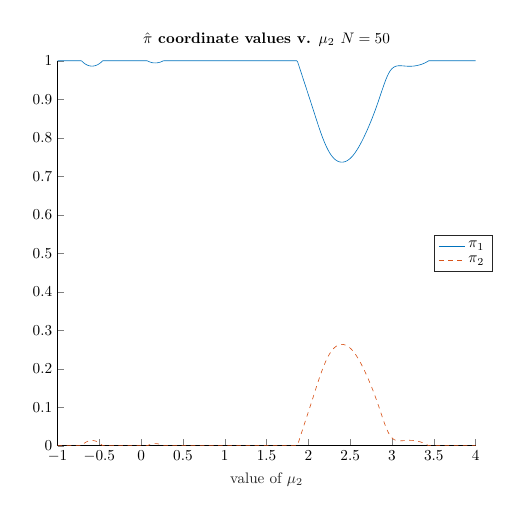
\begin{tikzpicture}[scale = .55]

\begin{axis}[%
width=3.8in,
height=3.5in,
at={(0in,0.481in)},
scale only axis,
xmin=-1,
xmax=4,
xlabel style={font=\color{white!15!black}},
xlabel={value of $\mu_2$},
ymin=0,
ymax=1,
axis background/.style={fill=white},
title style={font=\bfseries, align=center},
title={$\hat{\pi}$ coordinate values v. $\mu_2$ $N = 50$},
axis x line*=bottom,
axis y line*=left,
legend style={at={(.9,0.5)}, anchor=west, legend cell align=left, align=left, draw=white!15!black}
]
\addplot [color=mycolor1]
  table[row sep=crcr]{%
-1	0.999999999999834\\
-0.99	0.99999999999987\\
-0.98	0.999999999999884\\
-0.97	0.999999999999881\\
-0.96	0.999999999999861\\
-0.95	0.999999999999815\\
-0.94	0.999999999999728\\
-0.93	0.99999999999955\\
-0.92	0.99999999999972\\
-0.91	0.999999999999778\\
-0.9	0.999999999999441\\
-0.89	0.999999999999354\\
-0.88	0.999999999999586\\
-0.87	0.999999999999245\\
-0.86	0.999999999999157\\
-0.85	0.999999999999316\\
-0.84	0.999999999998614\\
-0.83	0.999999999998653\\
-0.82	0.999999999998699\\
-0.81	0.999999999997935\\
-0.8	0.999999999998097\\
-0.79	0.999999999997365\\
-0.78	0.999999999996373\\
-0.77	0.999999999995452\\
-0.76	0.99999999999464\\
-0.75	0.99999999999296\\
-0.74	0.999999999988789\\
-0.73	0.999999999981119\\
-0.72	0.999999999950619\\
-0.71	0.999254841354444\\
-0.7	0.997054801347346\\
-0.69	0.995088959737417\\
-0.68	0.993345390796756\\
-0.67	0.991813149572653\\
-0.66	0.990482329719492\\
-0.65	0.98934409295263\\
-0.64	0.98839067870958\\
-0.63	0.987615400862417\\
-0.62	0.987012636829877\\
-0.61	0.986577813199649\\
-0.6	0.986307390960983\\
-0.59	0.986198852664993\\
-0.58	0.986250693208328\\
-0.57	0.986462415511887\\
-0.56	0.986834531958297\\
-0.55	0.987368572270111\\
-0.54	0.988067098243911\\
-0.53	0.988933725682786\\
-0.52	0.989973153732887\\
-0.51	0.991191201741285\\
-0.5	0.992594853682326\\
-0.49	0.99419231005754\\
-0.48	0.995993046933471\\
-0.47	0.99800788138364\\
-0.46	0.999999999637399\\
-0.45	0.999999999967355\\
-0.44	0.999999999983912\\
-0.43	0.999999999989808\\
-0.42	0.999999999992438\\
-0.41	0.999999999994614\\
-0.4	0.999999999995302\\
-0.39	0.999999999996043\\
-0.38	0.999999999997204\\
-0.37	0.999999999997558\\
-0.36	0.999999999997791\\
-0.35	0.999999999998278\\
-0.34	0.999999999997928\\
-0.33	0.999999999998318\\
-0.32	0.999999999998805\\
-0.31	0.999999999998895\\
-0.3	0.99999999999867\\
-0.29	0.999999999998777\\
-0.28	0.999999999999204\\
-0.27	0.999999999998912\\
-0.26	0.99999999999899\\
-0.25	0.999999999998896\\
-0.24	0.999999999999229\\
-0.23	0.999999999998847\\
-0.22	0.999999999998923\\
-0.21	0.99999999999884\\
-0.2	0.999999999999223\\
-0.19	0.999999999998896\\
-0.18	0.999999999999011\\
-0.17	0.999999999998973\\
-0.16	0.999999999998772\\
-0.15	0.999999999999009\\
-0.14	0.999999999999048\\
-0.13	0.999999999998911\\
-0.12	0.999999999998533\\
-0.11	0.999999999998502\\
-0.1	0.999999999998123\\
-0.09	0.999999999998048\\
-0.08	0.999999999998185\\
-0.07	0.999999999997766\\
-0.0600000000000001	0.999999999997329\\
-0.05	0.99999999999746\\
-0.04	0.999999999996447\\
-0.03	0.999999999996229\\
-0.02	0.999999999995539\\
-0.01	0.999999999994439\\
0	0.999999999993471\\
0.01	0.99999999999246\\
0.02	0.999999999989797\\
0.03	0.999999999987156\\
0.04	0.999999999982433\\
0.05	0.999999999972865\\
0.0600000000000001	0.999999999950495\\
0.0700000000000001	0.999999999795732\\
0.0800000000000001	0.999248621992157\\
0.0900000000000001	0.998196137830576\\
0.1	0.997271370131328\\
0.11	0.996475019746401\\
0.12	0.99580722937482\\
0.13	0.995267678116553\\
0.14	0.994855676400888\\
0.15	0.994570255879791\\
0.16	0.994410250876115\\
0.17	0.994374369695469\\
0.18	0.994461255401345\\
0.19	0.994669536595194\\
0.2	0.994997869328404\\
0.21	0.995444971499255\\
0.22	0.996009651103349\\
0.23	0.99669082937852\\
0.24	0.997487559376633\\
0.25	0.998399039625388\\
0.26	0.999424621421674\\
0.27	0.999999999840001\\
0.28	0.99999999995078\\
0.29	0.999999999972409\\
0.3	0.999999999981111\\
0.31	0.999999999986335\\
0.32	0.999999999989146\\
0.33	0.999999999991102\\
0.34	0.999999999993094\\
0.35	0.999999999994057\\
0.36	0.999999999995041\\
0.37	0.999999999995552\\
0.38	0.999999999995505\\
0.39	0.999999999996288\\
0.4	0.999999999996573\\
0.41	0.999999999997414\\
0.42	0.999999999997493\\
0.43	0.999999999997684\\
0.44	0.999999999998073\\
0.45	0.999999999998075\\
0.46	0.999999999998393\\
0.47	0.999999999998448\\
0.48	0.999999999998263\\
0.49	0.99999999999852\\
0.5	0.999999999998594\\
0.51	0.999999999998513\\
0.52	0.999999999998902\\
0.53	0.999999999998588\\
0.54	0.999999999998775\\
0.55	0.999999999998857\\
0.56	0.99999999999886\\
0.57	0.999999999998785\\
0.58	0.999999999998621\\
0.59	0.999999999999029\\
0.6	0.999999999998773\\
0.61	0.999999999999057\\
0.62	0.999999999998687\\
0.63	0.999999999998907\\
0.64	0.999999999999058\\
0.65	0.999999999999162\\
0.66	0.99999999999923\\
0.67	0.999999999998717\\
0.68	0.999999999998756\\
0.69	0.999999999998763\\
0.7	0.999999999998745\\
0.71	0.999999999998702\\
0.72	0.999999999999223\\
0.73	0.999999999999167\\
0.74	0.999999999999096\\
0.75	0.999999999999006\\
0.76	0.999999999998898\\
0.77	0.999999999998766\\
0.78	0.999999999999198\\
0.79	0.999999999999091\\
0.8	0.999999999998967\\
0.81	0.999999999998824\\
0.82	0.999999999998662\\
0.83	0.999999999999111\\
0.84	0.99999999999899\\
0.85	0.999999999998861\\
0.86	0.999999999998725\\
0.87	0.999999999998582\\
0.88	0.999999999999075\\
0.89	0.999999999998991\\
0.9	0.999999999998914\\
0.91	0.999999999998845\\
0.92	0.999999999998792\\
0.93	0.999999999998755\\
0.94	0.99999999999874\\
0.95	0.999999999998745\\
0.96	0.999999999998772\\
0.97	0.999999999998821\\
0.98	0.999999999998889\\
0.99	0.999999999998971\\
1	0.999999999999065\\
1.01	0.999999999998594\\
1.02	0.999999999998762\\
1.03	0.999999999998929\\
1.04	0.999999999999089\\
1.05	0.99999999999869\\
1.06	0.999999999998908\\
1.07	0.999999999999101\\
1.08	0.999999999998724\\
1.09	0.99999999999896\\
1.1	0.999999999999157\\
1.11	0.999999999998798\\
1.12	0.99999999999902\\
1.13	0.9999999999992\\
1.14	0.999999999998823\\
1.15	0.99999999999902\\
1.16	0.999999999999175\\
1.17	0.999999999999295\\
1.18	0.999999999998886\\
1.19	0.999999999999009\\
1.2	0.9999999999991\\
1.21	0.999999999999164\\
1.22	0.999999999999203\\
1.23	0.999999999999217\\
1.24	0.99999999999921\\
1.25	0.999999999999177\\
1.26	0.999999999999117\\
1.27	0.999999999999021\\
1.28	0.99999999999888\\
1.29	0.999999999999274\\
1.3	0.999999999999113\\
1.31	0.999999999998886\\
1.32	0.999999999999195\\
1.33	0.999999999998926\\
1.34	0.999999999999168\\
1.35	0.999999999998833\\
1.36	0.999999999999035\\
1.37	0.999999999999177\\
1.38	0.999999999998774\\
1.39	0.999999999998906\\
1.4	0.999999999999\\
1.41	0.999999999998468\\
1.42	0.999999999998569\\
1.43	0.999999999998648\\
1.44	0.999999999998715\\
1.45	0.999999999998777\\
1.46	0.999999999998838\\
1.47	0.99999999999829\\
1.48	0.99999999999842\\
1.49	0.999999999998559\\
1.5	0.99999999999871\\
1.51	0.999999999998282\\
1.52	0.999999999998539\\
1.53	0.999999999998173\\
1.54	0.999999999998533\\
1.55	0.999999999998282\\
1.56	0.99999999999805\\
1.57	0.999999999998564\\
1.58	0.99999999999846\\
1.59	0.999999999998382\\
1.6	0.999999999998335\\
1.61	0.999999999998304\\
1.62	0.999999999998282\\
1.63	0.999999999998256\\
1.64	0.999999999998209\\
1.65	0.999999999998124\\
1.66	0.999999999997976\\
1.67	0.999999999998472\\
1.68	0.999999999998188\\
1.69	0.999999999998453\\
1.7	0.999999999998563\\
1.71	0.999999999998524\\
1.72	0.999999999998297\\
1.73	0.999999999997756\\
1.74	0.999999999998306\\
1.75	0.999999999997769\\
1.76	0.99999999999809\\
1.77	0.999999999997778\\
1.78	0.999999999997268\\
1.79	0.999999999996972\\
1.8	0.999999999996343\\
1.81	0.999999999996037\\
1.82	0.999999999995075\\
1.83	0.999999999993891\\
1.84	0.999999999991762\\
1.85	0.999999999985798\\
1.86	0.999999999964894\\
1.87	0.998061483549356\\
1.88	0.991641968759862\\
1.89	0.98507042906059\\
1.9	0.978418698383937\\
1.91	0.97173316960403\\
1.92	0.965042134946356\\
1.93	0.958361526830857\\
1.94	0.951698897278308\\
1.95	0.945056004719325\\
1.96	0.938430482991671\\
1.97	0.93181700126835\\
1.98	0.925208204015706\\
1.99	0.918595600302484\\
2	0.911970474580606\\
2.01	0.905324823187344\\
2.02	0.898652279766136\\
2.03	0.891948972141865\\
2.04	0.885214246298401\\
2.05	0.878451195492789\\
2.06	0.871666942462197\\
2.07	0.864872640289616\\
2.08	0.858083183204967\\
2.09	0.851316651303241\\
2.1	0.84459354853676\\
2.11	0.837935924109459\\
2.12	0.831366484776498\\
2.13	0.824907802650385\\
2.14	0.81858169820376\\
2.15	0.812408836349072\\
2.16	0.806408525571638\\
2.17	0.80059866900024\\
2.18	0.794995792595467\\
2.19	0.789615074204994\\
2.2	0.784470316171202\\
2.21	0.779573835929206\\
2.22	0.774936283368646\\
2.23	0.770566420932893\\
2.24	0.766470916217795\\
2.25	0.762654195737686\\
2.26	0.759118395461497\\
2.27	0.755863424297187\\
2.28	0.752887137000956\\
2.29	0.750185597516279\\
2.3	0.747753404830205\\
2.31	0.745584051004458\\
2.32	0.74367028371173\\
2.33	0.742004451256997\\
2.34	0.740578814814818\\
2.35	0.739385818989007\\
2.36	0.738418316990349\\
2.37	0.737669750365756\\
2.38	0.73713428534429\\
2.39	0.736806908692353\\
2.4	0.736683485811557\\
2.41	0.736760783004211\\
2.42	0.737036454711099\\
2.43	0.737508995428465\\
2.44	0.738177655268652\\
2.45	0.739042318067862\\
2.46	0.740103341860652\\
2.47	0.741361363647688\\
2.48	0.742817073732336\\
2.49	0.744470969304761\\
2.5	0.74632310186112\\
2.51	0.748372837608883\\
2.52	0.750618653033749\\
2.53	0.753057988085365\\
2.54	0.755687175974459\\
2.55	0.758501461076858\\
2.56	0.761495105541241\\
2.57	0.76466157261857\\
2.58	0.767993763041375\\
2.59	0.771484272730391\\
2.6	0.775125637968646\\
2.61	0.778910538900366\\
2.62	0.78283194315508\\
2.63	0.786883186272274\\
2.64	0.791058001051916\\
2.65	0.795350520382269\\
2.66	0.799755284346787\\
2.67	0.804267280781087\\
2.68	0.808882038945513\\
2.69	0.813595780535819\\
2.7	0.818405614413617\\
2.71	0.823309745296367\\
2.72	0.828307656025235\\
2.73	0.833400220046069\\
2.74	0.838589705600439\\
2.75	0.843879643868458\\
2.76	0.849274546950599\\
2.77	0.854779474939613\\
2.78	0.860399462190427\\
2.79	0.866138820424337\\
2.8	0.872000341109359\\
2.81	0.877984423211516\\
2.82	0.884088156750226\\
2.83	0.890304398806355\\
2.84	0.896620886547038\\
2.85	0.903019439346616\\
2.86	0.909475305357775\\
2.87	0.915956703599338\\
2.88	0.922424601577586\\
2.89	0.92883276100307\\
2.9	0.935128102176251\\
2.91	0.94125150577561\\
2.92	0.947139290727559\\
2.93	0.952725718101861\\
2.94	0.957946831552795\\
2.95	0.962745591551162\\
2.96	0.967077583159599\\
2.97	0.970915893299028\\
2.98	0.974253612320724\\
2.99	0.977103121318901\\
3	0.979492533378345\\
3.01	0.981460598447055\\
3.02	0.983051563390106\\
3.03	0.984311018968775\\
3.04	0.985283114266525\\
3.05	0.986009029518676\\
3.06	0.986526371534857\\
3.07	0.986869128929651\\
3.08	0.987067897272486\\
3.09	0.987150183881578\\
3.1	0.987140690820183\\
3.11	0.987061539242719\\
3.12	0.986932437378721\\
3.13	0.986770812208567\\
3.14	0.986591927869383\\
3.15	0.986409008337357\\
3.16	0.986233373613485\\
3.17	0.986074591028614\\
3.18	0.985940638164389\\
3.19	0.985838071523401\\
3.2	0.985772194929781\\
3.21	0.985747222830409\\
3.22	0.985766435396049\\
3.23	0.985832324091043\\
3.24	0.985946727767563\\
3.25	0.986110960251634\\
3.26	0.986325930859595\\
3.27	0.98659225929446\\
3.28	0.986910386101213\\
3.29	0.987280679421421\\
3.3	0.987703538279052\\
3.31	0.988179492193183\\
3.32	0.988709296600508\\
3.33	0.989294023444162\\
3.34	0.989935146354977\\
3.35	0.990634620114119\\
3.36	0.991394954442664\\
3.37	0.99221928260313\\
3.38	0.993111425779867\\
3.39	0.994075954569498\\
3.4	0.995118249273014\\
3.41	0.996244560898457\\
3.42	0.997462074927562\\
3.43	0.998778979965242\\
3.44	0.999999999774542\\
3.45	0.999999999974797\\
3.46	0.999999999987004\\
3.47	0.999999999992272\\
3.48	0.999999999994029\\
3.49	0.99999999999604\\
3.5	0.999999999996968\\
3.51	0.999999999997509\\
3.52	0.999999999997653\\
3.53	0.999999999998225\\
3.54	0.999999999998282\\
3.55	0.999999999998826\\
3.56	0.999999999998749\\
3.57	0.999999999998819\\
3.58	0.999999999999152\\
3.59	0.999999999999183\\
3.6	0.999999999999512\\
3.61	0.999999999999644\\
3.62	0.999999999999677\\
3.63	0.999999999999632\\
3.64	0.999999999999816\\
3.65	0.999999999999677\\
3.66	0.999999999999781\\
3.67	0.999999999999829\\
3.68	0.999999999999849\\
3.69	0.999999999999841\\
3.7	0.999999999999805\\
3.71	0.999999999999944\\
3.72	0.999999999999907\\
3.73	0.99999999999982\\
3.74	0.99999999999993\\
3.75	0.999999999999971\\
3.76	0.999999999999909\\
3.77	0.999999999999952\\
3.78	0.999999999999969\\
3.79	0.99999999999998\\
3.8	0.999999999999875\\
3.81	0.999999999999883\\
3.82	0.999999999999876\\
3.83	0.99999999999985\\
3.84	0.999999999999972\\
3.85	0.999999999999955\\
3.86	0.999999999999918\\
3.87	0.999999999999838\\
3.88	0.999999999999942\\
3.89	0.999999999999859\\
3.9	0.999999999999931\\
3.91	0.999999999999803\\
3.92	0.999999999999873\\
3.93	0.999999999999905\\
3.94	0.999999999999917\\
3.95	0.999999999999682\\
3.96	0.999999999999654\\
3.97	0.999999999999573\\
3.98	0.999999999999803\\
3.99	0.999999999999672\\
4	0.9999999999994\\
};
\addlegendentry{$\pi{}_\text{1}$}

\addplot [color=mycolor2, dashed]
  table[row sep=crcr]{%
-1	1.66605090370472e-13\\
-0.99	1.29555865073043e-13\\
-0.98	1.16186104021991e-13\\
-0.97	1.19361939920908e-13\\
-0.96	1.39430245865626e-13\\
-0.95	1.8403692589e-13\\
-0.94	2.72337837406396e-13\\
-0.93	4.49147391066927e-13\\
-0.92	2.79269393250927e-13\\
-0.91	2.2155234197073e-13\\
-0.9	5.59418786131788e-13\\
-0.89	6.45358278005196e-13\\
-0.88	4.13563775250456e-13\\
-0.87	7.54232230127119e-13\\
-0.86	8.42894299578229e-13\\
-0.85	6.83106636086315e-13\\
-0.84	1.38711184859745e-12\\
-0.83	1.34609308353339e-12\\
-0.82	1.30085134656642e-12\\
-0.81	2.06408203402325e-12\\
-0.8	1.90398590725774e-12\\
-0.79	2.6354763455273e-12\\
-0.78	3.62761126908215e-12\\
-0.77	4.54842294402851e-12\\
-0.76	5.35998497642118e-12\\
-0.75	7.04033840446348e-12\\
-0.74	1.12104608910724e-11\\
-0.73	1.88809533285668e-11\\
-0.72	4.93804509060709e-11\\
-0.71	0.000745158645556637\\
-0.7	0.00294519865265386\\
-0.69	0.00491104026258214\\
-0.68	0.00665460920324397\\
-0.67	0.00818685042734719\\
-0.66	0.00951767028050763\\
-0.65	0.0106559070473693\\
-0.64	0.0116093212904205\\
-0.63	0.0123845991375837\\
-0.62	0.0129873631701229\\
-0.61	0.0134221868003501\\
-0.6	0.0136926090390171\\
-0.59	0.0138011473350076\\
-0.58	0.0137493067916711\\
-0.57	0.0135375844881127\\
-0.56	0.0131654680417034\\
-0.55	0.0126314277298879\\
-0.54	0.0119329017560896\\
-0.53	0.0110662743172132\\
-0.52	0.0100268462671128\\
-0.51	0.00880879825871509\\
-0.5	0.00740514631767338\\
-0.49	0.00580768994245955\\
-0.48	0.00400695306652893\\
-0.47	0.00199211861636087\\
-0.46	3.62600632893764e-10\\
-0.45	3.26452158053593e-11\\
-0.44	1.60881877167359e-11\\
-0.43	1.01910144734131e-11\\
-0.42	7.56184974600157e-12\\
-0.41	5.38520773969831e-12\\
-0.4	4.6976947839358e-12\\
-0.39	3.95644656735876e-12\\
-0.38	2.79561707718715e-12\\
-0.37	2.44163520841684e-12\\
-0.36	2.20921284973032e-12\\
-0.35	1.72119067187168e-12\\
-0.34	2.07255467488096e-12\\
-0.33	1.6811247108796e-12\\
-0.32	1.19571494146551e-12\\
-0.31	1.10519774323493e-12\\
-0.3	1.33093310904149e-12\\
-0.29	1.22314313120346e-12\\
-0.28	7.96212910400901e-13\\
-0.27	1.08774517665273e-12\\
-0.26	1.00890658407967e-12\\
-0.25	1.10405580738451e-12\\
-0.24	7.7122223611294e-13\\
-0.23	1.15225797887691e-12\\
-0.22	1.0772750715419e-12\\
-0.21	1.15914776407281e-12\\
-0.2	7.78254478366019e-13\\
-0.19	1.10503403208789e-12\\
-0.18	9.89635227527242e-13\\
-0.17	1.02617825949422e-12\\
-0.16	1.22850306000624e-12\\
-0.15	9.9095561384984e-13\\
-0.14	9.52822635959541e-13\\
-0.13	1.08800605418554e-12\\
-0.12	1.46632733702261e-12\\
-0.11	1.4990951817518e-12\\
-0.1	1.87672058796575e-12\\
-0.09	1.95250412436775e-12\\
-0.08	1.81543922778987e-12\\
-0.07	2.23450247308846e-12\\
-0.0600000000000001	2.67181248195223e-12\\
-0.05	2.53957891506807e-12\\
-0.04	3.55359520734776e-12\\
-0.03	3.77148322830881e-12\\
-0.02	4.46032329120187e-12\\
-0.01	5.5621637318957e-12\\
0	6.52961346597986e-12\\
0.01	7.54024572252079e-12\\
0.02	1.02032393593375e-11\\
0.03	1.2844122612354e-11\\
0.04	1.75669801019474e-11\\
0.05	2.7134808336469e-11\\
0.0600000000000001	4.95056900754937e-11\\
0.0700000000000001	2.04267882339814e-10\\
0.0800000000000001	0.000751378007842992\\
0.0900000000000001	0.00180386216942431\\
0.1	0.00272862986867159\\
0.11	0.00352498025359993\\
0.12	0.00419277062517989\\
0.13	0.00473232188344704\\
0.14	0.0051443235991113\\
0.15	0.00542974412020897\\
0.16	0.00558974912388512\\
0.17	0.00562563030453177\\
0.18	0.00553874459865528\\
0.19	0.00533046340480566\\
0.2	0.00500213067159646\\
0.21	0.00455502850074458\\
0.22	0.00399034889665143\\
0.23	0.00330917062147972\\
0.24	0.00251244062336709\\
0.25	0.00160096037461221\\
0.26	0.000575378578325397\\
0.27	1.59999603875284e-10\\
0.28	4.92200215677824e-11\\
0.29	2.75912421190463e-11\\
0.3	1.88890913579999e-11\\
0.31	1.36643025669474e-11\\
0.32	1.08541387787214e-11\\
0.33	8.89707816208986e-12\\
0.34	6.90642405007872e-12\\
0.35	5.94294297880453e-12\\
0.36	4.95968577506422e-12\\
0.37	4.44741900125206e-12\\
0.38	4.4958742471508e-12\\
0.39	3.71167170823224e-12\\
0.4	3.42691396697659e-12\\
0.41	2.58630618377631e-12\\
0.42	2.50620822241123e-12\\
0.43	2.31574201440052e-12\\
0.44	1.92746377294531e-12\\
0.45	1.92486609224753e-12\\
0.46	1.6071367909522e-12\\
0.47	1.5530502288833e-12\\
0.48	1.73671600308856e-12\\
0.49	1.47952256261967e-12\\
0.5	1.40554942797424e-12\\
0.51	1.4867726031632e-12\\
0.52	1.09917011807241e-12\\
0.53	1.41095658797159e-12\\
0.54	1.22520690439439e-12\\
0.55	1.14185856760692e-12\\
0.56	1.13988753256719e-12\\
0.57	1.21529859245866e-12\\
0.58	1.37980817749314e-12\\
0.59	9.70313547935532e-13\\
0.6	1.22728842953628e-12\\
0.61	9.43199180188465e-13\\
0.62	1.31368907640549e-12\\
0.63	1.09333509398438e-12\\
0.64	9.41840334489996e-13\\
0.65	8.38284527999538e-13\\
0.66	7.69220940289262e-13\\
0.67	1.28286327207585e-12\\
0.68	1.24454706137124e-12\\
0.69	1.23626577784507e-12\\
0.7	1.2548820510392e-12\\
0.71	1.29851112815674e-12\\
0.72	7.76560335629481e-13\\
0.73	8.32245709689383e-13\\
0.74	9.04107110520544e-13\\
0.75	9.93787910994577e-13\\
0.76	1.10306454380031e-12\\
0.77	1.23411740700856e-12\\
0.78	8.0086497806183e-13\\
0.79	9.08478407128028e-13\\
0.8	1.0331768324497e-12\\
0.81	1.17637550134156e-12\\
0.82	1.33829925692378e-12\\
0.83	8.89658131680397e-13\\
0.84	1.00916172211396e-12\\
0.85	1.1385565945251e-12\\
0.86	1.27573925770405e-12\\
0.87	1.41751925520158e-12\\
0.88	9.25686414793808e-13\\
0.89	1.00941350489604e-12\\
0.9	1.08692994313542e-12\\
0.91	1.15429842025978e-12\\
0.92	1.20800247037532e-12\\
0.93	1.24455425695007e-12\\
0.94	1.26077318702114e-12\\
0.95	1.25538184153066e-12\\
0.96	1.2278726268038e-12\\
0.97	1.17918328449322e-12\\
0.98	1.11143331342778e-12\\
0.99	1.02857712459605e-12\\
1	9.34494102548465e-13\\
1.01	1.40715707054206e-12\\
1.02	1.23749471687697e-12\\
1.03	1.07030165680935e-12\\
1.04	9.11755054167896e-13\\
1.05	1.31074082236411e-12\\
1.06	1.09166065247004e-12\\
1.07	8.99355024608997e-13\\
1.08	1.27470643492306e-12\\
1.09	1.03903228019193e-12\\
1.1	8.42998453148847e-13\\
1.11	1.20282295240539e-12\\
1.12	9.79482297238925e-13\\
1.13	7.99879538070967e-13\\
1.14	1.1762615139785e-12\\
1.15	9.79463890154545e-13\\
1.16	8.24844075802742e-13\\
1.17	7.04440625964926e-13\\
1.18	1.11396643387485e-12\\
1.19	9.89863054703601e-13\\
1.2	8.98873383542919e-13\\
1.21	8.35724233108139e-13\\
1.22	7.97451390689834e-13\\
1.23	7.82447114087132e-13\\
1.24	7.90345560459384e-13\\
1.25	8.22823000410442e-13\\
1.26	8.83520896579745e-13\\
1.27	9.79042223158303e-13\\
1.28	1.11901652448511e-12\\
1.29	7.26841299700784e-13\\
1.3	8.86806078622647e-13\\
1.31	1.11374845762089e-12\\
1.32	8.05888573693501e-13\\
1.33	1.07362239241761e-12\\
1.34	8.3323492872905e-13\\
1.35	1.16821291383905e-12\\
1.36	9.65096621887513e-13\\
1.37	8.23212088156199e-13\\
1.38	1.22596411468799e-12\\
1.39	1.09447228510247e-12\\
1.4	9.99426962921821e-13\\
1.41	1.53159011901222e-12\\
1.42	1.4318978512381e-12\\
1.43	1.35249218499651e-12\\
1.44	1.28531905919823e-12\\
1.45	1.22333361578232e-12\\
1.46	1.16117167054678e-12\\
1.47	1.70956899168332e-12\\
1.48	1.58110761424429e-12\\
1.49	1.44111611034134e-12\\
1.5	1.28918854653178e-12\\
1.51	1.71903870297593e-12\\
1.52	1.46155363357373e-12\\
1.53	1.82747166174249e-12\\
1.54	1.46749952048453e-12\\
1.55	1.71921259511208e-12\\
1.56	1.9503262803637e-12\\
1.57	1.43627467549421e-12\\
1.58	1.54126764329762e-12\\
1.59	1.61680971033194e-12\\
1.6	1.66592430931837e-12\\
1.61	1.69614506874549e-12\\
1.62	1.71827956844963e-12\\
1.63	1.74474559476617e-12\\
1.64	1.79077133323072e-12\\
1.65	1.87563984722337e-12\\
1.66	2.0236948867416e-12\\
1.67	1.52795759897433e-12\\
1.68	1.81169949927319e-12\\
1.69	1.54684358523892e-12\\
1.7	1.43697549382157e-12\\
1.71	1.47613816374537e-12\\
1.72	1.70354212479673e-12\\
1.73	2.24347755529086e-12\\
1.74	1.69438761371449e-12\\
1.75	2.23171557293168e-12\\
1.76	1.91072985506984e-12\\
1.77	2.22206004498188e-12\\
1.78	2.73132351425516e-12\\
1.79	3.02809961425745e-12\\
1.8	3.65796407236933e-12\\
1.81	3.96317946820387e-12\\
1.82	4.92490077938287e-12\\
1.83	6.10914715014494e-12\\
1.84	8.23860225448585e-12\\
1.85	1.42024234219533e-11\\
1.86	3.51055478052102e-11\\
1.87	0.00193851645064415\\
1.88	0.00835803124013892\\
1.89	0.01492957093941\\
1.9	0.0215813016160637\\
1.91	0.0282668303959694\\
1.92	0.0349578650536431\\
1.93	0.041638473169144\\
1.94	0.0483011027216913\\
1.95	0.054943995280675\\
1.96	0.0615695170083286\\
1.97	0.0681829987316492\\
1.98	0.0747917959842939\\
1.99	0.0814043996975152\\
2	0.0880295254193945\\
2.01	0.0946751768126563\\
2.02	0.101347720233863\\
2.03	0.108051027858136\\
2.04	0.114785753701599\\
2.05	0.121548804507211\\
2.06	0.128333057537803\\
2.07	0.135127359710384\\
2.08	0.141916816795034\\
2.09	0.148683348696758\\
2.1	0.155406451463239\\
2.11	0.162064075890541\\
2.12	0.168633515223502\\
2.13	0.175092197349615\\
2.14	0.18141830179624\\
2.15	0.187591163650929\\
2.16	0.193591474428362\\
2.17	0.19940133099976\\
2.18	0.205004207404533\\
2.19	0.210384925795006\\
2.2	0.215529683828798\\
2.21	0.220426164070793\\
2.22	0.225063716631355\\
2.23	0.229433579067107\\
2.24	0.233529083782205\\
2.25	0.237345804262314\\
2.26	0.240881604538503\\
2.27	0.244136575702813\\
2.28	0.247112862999044\\
2.29	0.24981440248372\\
2.3	0.252246595169795\\
2.31	0.254415948995542\\
2.32	0.25632971628827\\
2.33	0.257995548743003\\
2.34	0.259421185185182\\
2.35	0.260614181010993\\
2.36	0.261581683009651\\
2.37	0.262330249634245\\
2.38	0.26286571465571\\
2.39	0.263193091307647\\
2.4	0.263316514188443\\
2.41	0.263239216995789\\
2.42	0.262963545288901\\
2.43	0.262491004571535\\
2.44	0.261822344731348\\
2.45	0.260957681932138\\
2.46	0.259896658139347\\
2.47	0.258638636352312\\
2.48	0.257182926267664\\
2.49	0.255529030695239\\
2.5	0.25367689813888\\
2.51	0.251627162391117\\
2.52	0.249381346966251\\
2.53	0.246942011914635\\
2.54	0.244312824025541\\
2.55	0.241498538923142\\
2.56	0.238504894458758\\
2.57	0.23533842738143\\
2.58	0.232006236958625\\
2.59	0.228515727269609\\
2.6	0.224874362031354\\
2.61	0.221089461099633\\
2.62	0.21716805684492\\
2.63	0.213116813727726\\
2.64	0.208941998948085\\
2.65	0.204649479617731\\
2.66	0.200244715653213\\
2.67	0.195732719218914\\
2.68	0.191117961054488\\
2.69	0.18640421946418\\
2.7	0.181594385586384\\
2.71	0.176690254703633\\
2.72	0.171692343974765\\
2.73	0.166599779953931\\
2.74	0.161410294399561\\
2.75	0.156120356131542\\
2.76	0.150725453049401\\
2.77	0.145220525060387\\
2.78	0.139600537809572\\
2.79	0.133861179575662\\
2.8	0.127999658890642\\
2.81	0.122015576788484\\
2.82	0.115911843249774\\
2.83	0.109695601193644\\
2.84	0.103379113452962\\
2.85	0.0969805606533835\\
2.86	0.0905246946422249\\
2.87	0.0840432964006633\\
2.88	0.0775753984224152\\
2.89	0.0711672389969307\\
2.9	0.0648718978237485\\
2.91	0.05874849422439\\
2.92	0.052860709272441\\
2.93	0.0472742818981381\\
2.94	0.0420531684472053\\
2.95	0.037254408448839\\
2.96	0.0329224168404017\\
2.97	0.0290841067009719\\
2.98	0.0257463876792756\\
2.99	0.0228968786810994\\
3	0.020507466621654\\
3.01	0.0185394015529455\\
3.02	0.0169484366098934\\
3.03	0.015688981031225\\
3.04	0.0147168857334751\\
3.05	0.0139909704813239\\
3.06	0.0134736284651425\\
3.07	0.01313087107035\\
3.08	0.0129321027275149\\
3.09	0.0128498161184214\\
3.1	0.0128593091798161\\
3.11	0.0129384607572801\\
3.12	0.0130675626212796\\
3.13	0.0132291877914334\\
3.14	0.0134080721306171\\
3.15	0.0135909916626437\\
3.16	0.0137666263865146\\
3.17	0.0139254089713865\\
3.18	0.0140593618356108\\
3.19	0.0141619284765985\\
3.2	0.0142278050702188\\
3.21	0.0142527771695907\\
3.22	0.0142335646039508\\
3.23	0.0141676759089567\\
3.24	0.0140532722324382\\
3.25	0.0138890397483666\\
3.26	0.0136740691404057\\
3.27	0.0134077407055391\\
3.28	0.0130896138987864\\
3.29	0.0127193205785784\\
3.3	0.0122964617209481\\
3.31	0.0118205078068171\\
3.32	0.0112907033994919\\
3.33	0.0107059765558376\\
3.34	0.0100648536450235\\
3.35	0.00936537988588055\\
3.36	0.00860504555733602\\
3.37	0.00778071739687004\\
3.38	0.00688857422013279\\
3.39	0.005924045430501\\
3.4	0.00488175072698665\\
3.41	0.00375543910154224\\
3.42	0.00253792507243798\\
3.43	0.00122102003475776\\
3.44	2.25456820135553e-10\\
3.45	2.52030176194231e-11\\
3.46	1.29972205146035e-11\\
3.47	7.72793741206707e-12\\
3.48	5.97115815430855e-12\\
3.49	3.95921232380657e-12\\
3.5	3.03191155332184e-12\\
3.51	2.49086705836334e-12\\
3.52	2.34750242439816e-12\\
3.53	1.77500230213037e-12\\
3.54	1.71898610061019e-12\\
3.55	1.17324226120143e-12\\
3.56	1.25155897797694e-12\\
3.57	1.1803547361487e-12\\
3.58	8.47426859646407e-13\\
3.59	8.16613723205618e-13\\
3.6	4.87191695625441e-13\\
3.61	3.55588351001231e-13\\
3.62	3.22472275245198e-13\\
3.63	3.68482763911684e-13\\
3.64	1.83723971427196e-13\\
3.65	3.23470344031221e-13\\
3.66	2.19655750143873e-13\\
3.67	1.70400062927268e-13\\
3.68	1.52512312373312e-13\\
3.69	1.58925118898802e-13\\
3.7	1.94715378967973e-13\\
3.71	5.71296746489972e-14\\
3.72	9.22286724854388e-14\\
3.73	1.79671919585495e-13\\
3.74	6.98857402854822e-14\\
3.75	2.93354383337983e-14\\
3.76	9.15685505255765e-14\\
3.77	4.92416385804115e-14\\
3.78	2.98261652868734e-14\\
3.79	2.0594200535397e-14\\
3.8	1.25306610885682e-13\\
3.81	1.16029591816908e-13\\
3.82	1.23301654319616e-13\\
3.83	1.4982556491047e-13\\
3.84	2.83421547451562e-14\\
3.85	4.55994960480689e-14\\
3.86	8.1987202061677e-14\\
3.87	1.62423732982454e-13\\
3.88	5.78889805286748e-14\\
3.89	1.41204927343179e-13\\
3.9	6.86262486497088e-14\\
3.91	1.97281412600222e-13\\
3.92	1.26661510654574e-13\\
3.93	9.56580154652212e-14\\
3.94	8.41498583637435e-14\\
3.95	3.18735214127629e-13\\
3.96	3.45993968528334e-13\\
3.97	4.26705996651677e-13\\
3.98	1.96832515186063e-13\\
3.99	3.2682677442361e-13\\
4	5.99918479910661e-13\\
};
\addlegendentry{$\pi{}_\text{2}$}

\end{axis}
\end{tikzpicture}%
			}
			%	\qquad
			\subcaptionbox{Here \( N=500 \). Ratios of the samples of the clusters are \( \pi_1^\ast =0.8 \) and \( \pi_2^\ast =0.2 \). \label{fig:gmmExampleK2sub2}}[.4\linewidth]{
				% This file was created by matlab2tikz.
%
%The latest updates can be retrieved from
%  http://www.mathworks.com/matlabcentral/fileexchange/22022-matlab2tikz-matlab2tikz
%where you can also make suggestions and rate matlab2tikz.
%
\definecolor{mycolor1}{rgb}{0.00000,0.44700,0.74100}%
\definecolor{mycolor2}{rgb}{0.85000,0.32500,0.09800}%
%
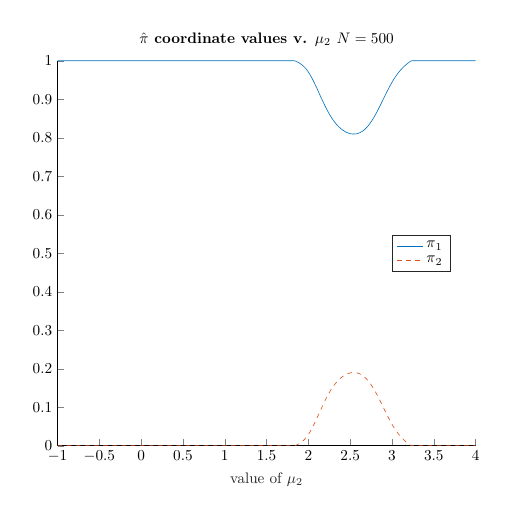
\begin{tikzpicture}[scale = .55]

\begin{axis}[%
width=3.8in,
height=3.5in,
at={(0in,0.481in)},
scale only axis,
xmin=-1,
xmax=4,
xlabel style={font=\color{white!15!black}},
xlabel={value of $\mu_2$},
ymin=0,
ymax=1,
axis background/.style={fill=white},
title style={font=\bfseries, align=center},
title={$\hat{\pi}$ coordinate values v. $\mu_2$ $N = 500$},
axis x line*=bottom,
axis y line*=left,
legend style={at={(.8,0.5)}, anchor=west, legend cell align=left, align=left, draw=white!15!black}
]
\addplot [color=mycolor1]
  table[row sep=crcr]{%
-1	0.999999999994316\\
-0.99	0.999999999994807\\
-0.98	0.999999999995185\\
-0.97	0.999999999995603\\
-0.96	0.999999999995345\\
-0.95	0.999999999996177\\
-0.94	0.99999999999569\\
-0.93	0.999999999996443\\
-0.92	0.99999999999679\\
-0.91	0.999999999996841\\
-0.9	0.999999999996623\\
-0.89	0.999999999996944\\
-0.88	0.999999999997047\\
-0.87	0.999999999996974\\
-0.86	0.999999999996714\\
-0.85	0.999999999997116\\
-0.84	0.99999999999737\\
-0.83	0.999999999997505\\
-0.82	0.999999999997556\\
-0.81	0.999999999997527\\
-0.8	0.999999999997433\\
-0.79	0.999999999997272\\
-0.78	0.999999999997045\\
-0.77	0.999999999997572\\
-0.76	0.999999999997298\\
-0.75	0.999999999997745\\
-0.74	0.999999999997455\\
-0.73	0.999999999997869\\
-0.72	0.99999999999759\\
-0.71	0.999999999997274\\
-0.7	0.999999999997746\\
-0.69	0.99999999999748\\
-0.68	0.99999999999796\\
-0.67	0.999999999997754\\
-0.66	0.999999999997553\\
-0.65	0.99999999999809\\
-0.64	0.999999999997965\\
-0.63	0.999999999997846\\
-0.62	0.999999999997745\\
-0.61	0.999999999997652\\
-0.6	0.999999999998287\\
-0.59	0.999999999998248\\
-0.58	0.999999999998212\\
-0.57	0.999999999998182\\
-0.56	0.999999999998155\\
-0.55	0.999999999998119\\
-0.54	0.999999999998078\\
-0.53	0.999999999998022\\
-0.52	0.999999999997946\\
-0.51	0.999999999998554\\
-0.5	0.999999999998475\\
-0.49	0.999999999998366\\
-0.48	0.999999999998217\\
-0.47	0.999999999998703\\
-0.46	0.999999999998534\\
-0.45	0.999999999998308\\
-0.44	0.99999999999871\\
-0.43	0.999999999998446\\
-0.42	0.999999999998771\\
-0.41	0.999999999998441\\
-0.4	0.999999999998714\\
-0.39	0.999999999998915\\
-0.38	0.999999999998512\\
-0.37	0.999999999998685\\
-0.36	0.999999999998805\\
-0.35	0.999999999998893\\
-0.34	0.999999999998946\\
-0.33	0.99999999999835\\
-0.32	0.99999999999835\\
-0.31	0.999999999998944\\
-0.3	0.999999999998893\\
-0.29	0.999999999998814\\
-0.28	0.999999999998695\\
-0.27	0.999999999998534\\
-0.26	0.999999999998314\\
-0.25	0.999999999998754\\
-0.24	0.999999999998508\\
-0.23	0.99999999999884\\
-0.22	0.999999999998546\\
-0.21	0.999999999998817\\
-0.2	0.999999999998464\\
-0.19	0.999999999998683\\
-0.18	0.999999999998226\\
-0.17	0.99999999999841\\
-0.16	0.999999999998536\\
-0.15	0.999999999998621\\
-0.14	0.999999999997999\\
-0.13	0.999999999998021\\
-0.12	0.999999999997993\\
-0.11	0.999999999997906\\
-0.1	0.999999999998456\\
-0.09	0.999999999998291\\
-0.08	0.999999999998055\\
-0.07	0.999999999997725\\
-0.0600000000000001	0.999999999998062\\
-0.05	0.999999999997586\\
-0.04	0.999999999997769\\
-0.03	0.999999999997847\\
-0.02	0.999999999997834\\
-0.01	0.999999999997721\\
0	0.999999999997502\\
0.01	0.999999999997147\\
0.02	0.999999999997415\\
0.03	0.999999999996781\\
0.04	0.999999999996774\\
0.05	0.999999999996596\\
0.0600000000000001	0.999999999996231\\
0.0700000000000001	0.999999999996511\\
0.0800000000000001	0.999999999996576\\
0.0900000000000001	0.999999999996448\\
0.1	0.99999999999613\\
0.11	0.999999999995601\\
0.12	0.99999999999567\\
0.13	0.999999999995543\\
0.14	0.99999999999524\\
0.15	0.999999999994756\\
0.16	0.999999999994116\\
0.17	0.999999999994235\\
0.18	0.999999999993414\\
0.19	0.999999999993497\\
0.2	0.999999999993645\\
0.21	0.999999999993108\\
0.22	0.99999999999284\\
0.23	0.999999999992055\\
0.24	0.999999999992665\\
0.25	0.999999999992111\\
0.26	0.999999999992246\\
0.27	0.999999999992272\\
0.28	0.999999999992254\\
0.29	0.999999999992219\\
0.3	0.999999999992169\\
0.31	0.999999999992064\\
0.32	0.999999999991841\\
0.33	0.999999999992326\\
0.34	0.999999999992513\\
0.35	0.999999999992294\\
0.36	0.999999999993345\\
0.37	0.99999999999291\\
0.38	0.999999999993523\\
0.39	0.999999999994186\\
0.4	0.999999999994014\\
0.41	0.999999999994618\\
0.42	0.999999999994256\\
0.43	0.999999999994605\\
0.44	0.999999999994757\\
0.45	0.999999999995557\\
0.46	0.999999999995298\\
0.47	0.999999999995653\\
0.48	0.999999999995775\\
0.49	0.999999999996475\\
0.5	0.999999999996173\\
0.51	0.999999999996451\\
0.52	0.999999999996525\\
0.53	0.999999999996381\\
0.54	0.999999999996868\\
0.55	0.999999999997143\\
0.56	0.999999999997254\\
0.57	0.999999999997202\\
0.58	0.99999999999698\\
0.59	0.999999999997381\\
0.6	0.999999999997612\\
0.61	0.999999999997709\\
0.62	0.999999999997682\\
0.63	0.999999999997531\\
0.64	0.999999999997221\\
0.65	0.999999999997558\\
0.66	0.999999999997745\\
0.67	0.999999999997816\\
0.68	0.999999999997772\\
0.69	0.999999999997612\\
0.7	0.999999999997315\\
0.71	0.999999999997636\\
0.72	0.99999999999707\\
0.73	0.999999999997154\\
0.74	0.999999999997094\\
0.75	0.999999999997632\\
0.76	0.999999999997315\\
0.77	0.9999999999968\\
0.78	0.999999999996925\\
0.79	0.999999999996871\\
0.8	0.999999999996634\\
0.81	0.999999999997\\
0.82	0.999999999996376\\
0.83	0.999999999996326\\
0.84	0.999999999996032\\
0.85	0.99999999999631\\
0.86	0.99999999999629\\
0.87	0.999999999995986\\
0.88	0.999999999995343\\
0.89	0.999999999995154\\
0.9	0.999999999995392\\
0.91	0.999999999994342\\
0.92	0.999999999994511\\
0.93	0.999999999994107\\
0.94	0.999999999993937\\
0.95	0.999999999993084\\
0.96	0.999999999993189\\
0.97	0.999999999992442\\
0.98	0.999999999991592\\
0.99	0.999999999990528\\
1	0.999999999990072\\
1.01	0.999999999989153\\
1.02	0.999999999988575\\
1.03	0.999999999987283\\
1.04	0.999999999986091\\
1.05	0.999999999984929\\
1.06	0.999999999983774\\
1.07	0.999999999982705\\
1.08	0.999999999981003\\
1.09	0.999999999979083\\
1.1	0.99999999997762\\
1.11	0.99999999997569\\
1.12	0.999999999973631\\
1.13	0.999999999973015\\
1.14	0.999999999971652\\
1.15	0.999999999971092\\
1.16	0.999999999970545\\
1.17	0.999999999970497\\
1.18	0.999999999971638\\
1.19	0.999999999972957\\
1.2	0.999999999973919\\
1.21	0.999999999975693\\
1.22	0.99999999997758\\
1.23	0.999999999979105\\
1.24	0.999999999981081\\
1.25	0.999999999982728\\
1.26	0.999999999983564\\
1.27	0.999999999985243\\
1.28	0.999999999986703\\
1.29	0.999999999987977\\
1.3	0.999999999989146\\
1.31	0.999999999989439\\
1.32	0.999999999990811\\
1.33	0.999999999991584\\
1.34	0.999999999991929\\
1.35	0.999999999991961\\
1.36	0.999999999992707\\
1.37	0.999999999993372\\
1.38	0.999999999994037\\
1.39	0.999999999993967\\
1.4	0.999999999994062\\
1.41	0.999999999994406\\
1.42	0.999999999995039\\
1.43	0.999999999995167\\
1.44	0.999999999994835\\
1.45	0.999999999994924\\
1.46	0.999999999995468\\
1.47	0.999999999995638\\
1.48	0.999999999995468\\
1.49	0.999999999995805\\
1.5	0.999999999995835\\
1.51	0.999999999995568\\
1.52	0.999999999995843\\
1.53	0.99999999999584\\
1.54	0.999999999995554\\
1.55	0.999999999995824\\
1.56	0.999999999995809\\
1.57	0.999999999995517\\
1.58	0.999999999995745\\
1.59	0.999999999995679\\
1.6	0.999999999995298\\
1.61	0.999999999995395\\
1.62	0.999999999995137\\
1.63	0.999999999994454\\
1.64	0.999999999994178\\
1.65	0.99999999999428\\
1.66	0.999999999993794\\
1.67	0.99999999999354\\
1.68	0.999999999993409\\
1.69	0.99999999999327\\
1.7	0.999999999992959\\
1.71	0.999999999992273\\
1.72	0.999999999991773\\
1.73	0.999999999991076\\
1.74	0.99999999998961\\
1.75	0.999999999988336\\
1.76	0.999999999986939\\
1.77	0.999999999985277\\
1.78	0.999999999982812\\
1.79	0.999999999980082\\
1.8	0.99999999997434\\
1.81	0.999999999966228\\
1.82	0.999999999947826\\
1.83	0.999999999884668\\
1.84	0.999834706436207\\
1.85	0.998877505501881\\
1.86	0.997859254332665\\
1.87	0.996771166399231\\
1.88	0.995603375725643\\
1.89	0.994344941057559\\
1.9	0.992983886290174\\
1.91	0.991507289410681\\
1.92	0.989901433900123\\
1.93	0.988152037615977\\
1.94	0.986244573359053\\
1.95	0.984164691639423\\
1.96	0.981898748437242\\
1.97	0.979434428146065\\
1.98	0.976761434477977\\
1.99	0.973872201723835\\
2	0.970762559154772\\
2.01	0.96743226865223\\
2.02	0.96388535613689\\
2.03	0.960130175547563\\
2.04	0.956179179146982\\
2.05	0.952048412988893\\
2.06	0.947756799867102\\
2.07	0.943325302131146\\
2.08	0.938776066285902\\
2.09	0.934131639958917\\
2.1	0.929414325659101\\
2.11	0.924645703602221\\
2.12	0.919846325715457\\
2.13	0.915035560056282\\
2.14	0.910231551121985\\
2.15	0.90545125644285\\
2.16	0.900710521541893\\
2.17	0.896024161558373\\
2.18	0.891406026419468\\
2.19	0.886869035686235\\
2.2	0.882425177791201\\
2.21	0.878085475619767\\
2.22	0.873859925777663\\
2.23	0.869757422412729\\
2.24	0.865785678133329\\
2.25	0.861951154623382\\
2.26	0.858259014188648\\
2.27	0.854713101004654\\
2.28	0.851315957660908\\
2.29	0.848068879093475\\
2.3	0.844972002636119\\
2.31	0.842024430077402\\
2.32	0.839224375507701\\
2.33	0.836569331513395\\
2.34	0.834056245829063\\
2.35	0.831681700714405\\
2.36	0.829442087936317\\
2.37	0.82733377303402\\
2.38	0.825353243506243\\
2.39	0.823497236539336\\
2.4	0.821762842955786\\
2.41	0.820147585213728\\
2.42	0.818649468535343\\
2.43	0.817267005606831\\
2.44	0.815999216724039\\
2.45	0.814845608635708\\
2.46	0.813806136568573\\
2.47	0.812881154823121\\
2.48	0.812071361812811\\
2.49	0.811377745354829\\
2.5	0.810801533428214\\
2.51	0.810344154524168\\
2.52	0.810007210259237\\
2.53	0.809792461270576\\
2.54	0.809701825746549\\
2.55	0.809737388432124\\
2.56	0.809901416713751\\
2.57	0.810196379509611\\
2.58	0.810624964198171\\
2.59	0.811190086702856\\
2.6	0.811894890084828\\
2.61	0.812742727541979\\
2.62	0.813737126533814\\
2.63	0.814881731816434\\
2.64	0.816180226441671\\
2.65	0.817636231224622\\
2.66	0.819253184726701\\
2.67	0.821034207409258\\
2.68	0.822981955134527\\
2.69	0.825098468547232\\
2.7	0.827385025872163\\
2.71	0.829842007213517\\
2.72	0.832468778376797\\
2.73	0.835263601452315\\
2.74	0.838223577927743\\
2.75	0.841344627919624\\
2.76	0.844621506462689\\
2.77	0.848047854890968\\
2.78	0.851616282485863\\
2.79	0.855318471151755\\
2.8	0.859145294090357\\
2.81	0.863086938583367\\
2.82	0.867133023038462\\
2.83	0.871272699462695\\
2.84	0.875494734421508\\
2.85	0.879787564187275\\
2.86	0.884139323143757\\
2.87	0.888537848319737\\
2.88	0.892970666964696\\
2.89	0.897424977855536\\
2.9	0.901887640040588\\
2.91	0.906345184322452\\
2.92	0.910783862483567\\
2.93	0.915189746680344\\
2.94	0.919548886528383\\
2.95	0.923847524464307\\
2.96	0.928072361686516\\
2.97	0.932210858452271\\
2.98	0.936251545088566\\
2.99	0.940184315314075\\
3	0.944000672588374\\
3.01	0.947693903829054\\
3.02	0.951259162738539\\
3.03	0.954693455767504\\
3.04	0.957995535496947\\
3.05	0.961165716728169\\
3.06	0.964205638120005\\
3.07	0.967117995886471\\
3.08	0.969906275865839\\
3.09	0.972574506826605\\
3.1	0.975127052156116\\
3.11	0.977568450143544\\
3.12	0.979903305727464\\
3.13	0.982136229626866\\
3.14	0.984271814921478\\
3.15	0.986314636922294\\
3.16	0.988269260171899\\
3.17	0.990140236811989\\
3.18	0.991932083250881\\
3.19	0.993649226440989\\
3.2	0.99529591636237\\
3.21	0.996876106529587\\
3.22	0.998393308902086\\
3.23	0.999850432820997\\
3.24	0.999999999951323\\
3.25	0.999999999977877\\
3.26	0.999999999985575\\
3.27	0.999999999989163\\
3.28	0.999999999991162\\
3.29	0.999999999992711\\
3.3	0.99999999999392\\
3.31	0.999999999994867\\
3.32	0.999999999995333\\
3.33	0.999999999996187\\
3.34	0.999999999996361\\
3.35	0.999999999996992\\
3.36	0.999999999996798\\
3.37	0.999999999997469\\
3.38	0.999999999997622\\
3.39	0.999999999997374\\
3.4	0.999999999997516\\
3.41	0.999999999998085\\
3.42	0.999999999997743\\
3.43	0.999999999997907\\
3.44	0.9999999999979\\
3.45	0.999999999998431\\
3.46	0.999999999998208\\
3.47	0.999999999998526\\
3.48	0.999999999998119\\
3.49	0.999999999998316\\
3.5	0.999999999998442\\
3.51	0.999999999998519\\
3.52	0.999999999998557\\
3.53	0.999999999998566\\
3.54	0.999999999998544\\
3.55	0.999999999998491\\
3.56	0.999999999998418\\
3.57	0.999999999998954\\
3.58	0.999999999998881\\
3.59	0.999999999998794\\
3.6	0.999999999998682\\
3.61	0.999999999998543\\
3.62	0.999999999999027\\
3.63	0.999999999998914\\
3.64	0.999999999998765\\
3.65	0.999999999999178\\
3.66	0.999999999999048\\
3.67	0.999999999998888\\
3.68	0.999999999999253\\
3.69	0.999999999999097\\
3.7	0.99999999999889\\
3.71	0.999999999999236\\
3.72	0.99999999999902\\
3.73	0.999999999999315\\
3.74	0.999999999999078\\
3.75	0.999999999999335\\
3.76	0.999999999999056\\
3.77	0.99999999999929\\
3.78	0.999999999999456\\
3.79	0.999999999999159\\
3.8	0.999999999999319\\
3.81	0.999999999999436\\
3.82	0.999999999999037\\
3.83	0.999999999999152\\
3.84	0.99999999999923\\
3.85	0.999999999999283\\
3.86	0.999999999999305\\
3.87	0.999999999999306\\
3.88	0.999999999999281\\
3.89	0.999999999999237\\
3.9	0.999999999999159\\
3.91	0.999999999999044\\
3.92	0.999999999999435\\
3.93	0.999999999999313\\
3.94	0.999999999999138\\
3.95	0.99999999999943\\
3.96	0.999999999999245\\
3.97	0.999999999998977\\
3.98	0.999999999999257\\
3.99	0.999999999998946\\
4	0.999999999999179\\
};
\addlegendentry{$\pi{}_\text{1}$}

\addplot [color=mycolor2, dashed]
  table[row sep=crcr]{%
-1	5.68164610883259e-12\\
-0.99	5.19237920784404e-12\\
-0.98	4.81400389612833e-12\\
-0.97	4.39799179870542e-12\\
-0.96	4.65582614777294e-12\\
-0.95	3.8217031653439e-12\\
-0.94	4.3079397153306e-12\\
-0.93	3.55950528433036e-12\\
-0.92	3.21195219682789e-12\\
-0.91	3.15898954701126e-12\\
-0.9	3.3768323383652e-12\\
-0.89	3.05787275093081e-12\\
-0.88	2.95143617736076e-12\\
-0.87	3.02691022485471e-12\\
-0.86	3.2864329540688e-12\\
-0.85	2.88183130045055e-12\\
-0.84	2.63141885892618e-12\\
-0.83	2.49361890762835e-12\\
-0.82	2.44518631820639e-12\\
-0.81	2.471865531381e-12\\
-0.8	2.56688315003795e-12\\
-0.79	2.72795881951704e-12\\
-0.78	2.95644415858725e-12\\
-0.77	2.42927961596463e-12\\
-0.76	2.70368661177682e-12\\
-0.75	2.25592967456073e-12\\
-0.74	2.54613413715189e-12\\
-0.73	2.13176000293972e-12\\
-0.72	2.41212507414705e-12\\
-0.71	2.72619198585167e-12\\
-0.7	2.25319145685002e-12\\
-0.69	2.51897126864714e-12\\
-0.68	2.0412862719492e-12\\
-0.67	2.24400852892718e-12\\
-0.66	2.44573158892403e-12\\
-0.65	1.90839322921735e-12\\
-0.64	2.03564012806749e-12\\
-0.63	2.15205962647456e-12\\
-0.62	2.25627221882969e-12\\
-0.61	2.34695596333655e-12\\
-0.6	1.71449483747497e-12\\
-0.59	1.75397552128301e-12\\
-0.58	1.78737891384764e-12\\
-0.57	1.8175300081188e-12\\
-0.56	1.84761601555223e-12\\
-0.55	1.88144303129982e-12\\
-0.54	1.92391433032448e-12\\
-0.53	1.97912392887526e-12\\
-0.52	2.05375051900991e-12\\
-0.51	1.44484057231242e-12\\
-0.5	1.5256606335006e-12\\
-0.49	1.63529178607508e-12\\
-0.48	1.7832689744201e-12\\
-0.47	1.29793454812349e-12\\
-0.46	1.46476101779297e-12\\
-0.45	1.69149657815696e-12\\
-0.44	1.28849972690965e-12\\
-0.43	1.55539397415294e-12\\
-0.42	1.23018653147806e-12\\
-0.41	1.56027307098556e-12\\
-0.4	1.28792207961655e-12\\
-0.39	1.08586711971525e-12\\
-0.38	1.48917772286926e-12\\
-0.37	1.31787449203547e-12\\
-0.36	1.19418045095613e-12\\
-0.35	1.10866650846566e-12\\
-0.34	1.05471631345524e-12\\
-0.33	1.64847893755168e-12\\
-0.32	1.64834953650938e-12\\
-0.31	1.05353129088391e-12\\
-0.3	1.10551254853221e-12\\
-0.29	1.18752486401055e-12\\
-0.28	1.3053732914743e-12\\
-0.27	1.46660344731185e-12\\
-0.26	1.683323258562e-12\\
-0.25	1.24677871199247e-12\\
-0.24	1.49395583546117e-12\\
-0.23	1.16259799055015e-12\\
-0.22	1.45150303554667e-12\\
-0.21	1.18528793500016e-12\\
-0.2	1.5379748018148e-12\\
-0.19	1.31681187236007e-12\\
-0.18	1.77159823660595e-12\\
-0.17	1.58870521004996e-12\\
-0.16	1.46187491416101e-12\\
-0.15	1.3809877631231e-12\\
-0.14	2.00004779390853e-12\\
-0.13	1.9772967738631e-12\\
-0.12	2.00723618855101e-12\\
-0.11	2.09210688923133e-12\\
-0.1	1.54162633364732e-12\\
-0.09	1.7076894639749e-12\\
-0.08	1.94349779290635e-12\\
-0.07	2.27278657643869e-12\\
-0.0600000000000001	1.94013545949115e-12\\
-0.05	2.4145070640253e-12\\
-0.04	2.22974258954009e-12\\
-0.03	2.15047327053095e-12\\
-0.02	2.1660593557944e-12\\
-0.01	2.27728832411076e-12\\
0	2.49671770231416e-12\\
0.01	2.85197913629065e-12\\
0.02	2.58329853283306e-12\\
0.03	3.21752064413553e-12\\
0.04	3.22491077208989e-12\\
0.05	3.40360293816642e-12\\
0.0600000000000001	3.77165255992325e-12\\
0.0700000000000001	3.48945647088291e-12\\
0.0800000000000001	3.42589069180414e-12\\
0.0900000000000001	3.55210064012816e-12\\
0.1	3.86869771526816e-12\\
0.11	4.40118632054583e-12\\
0.12	4.32706298646023e-12\\
0.13	4.454742689445e-12\\
0.14	4.762706199427e-12\\
0.15	5.24220137476788e-12\\
0.16	5.88612332178603e-12\\
0.17	5.76546407308871e-12\\
0.18	6.58473404329488e-12\\
0.19	6.50181804375433e-12\\
0.2	6.35556441539291e-12\\
0.21	6.8905506551287e-12\\
0.22	7.16151365634128e-12\\
0.23	7.94677144954887e-12\\
0.24	7.33411532362548e-12\\
0.25	7.88785234989517e-12\\
0.26	7.75351173635469e-12\\
0.27	7.72613228691591e-12\\
0.28	7.74437658828787e-12\\
0.29	7.77931823842644e-12\\
0.3	7.8322689821364e-12\\
0.31	7.93649056818463e-12\\
0.32	8.15929020165211e-12\\
0.33	7.67587638592918e-12\\
0.34	7.48768355919035e-12\\
0.35	7.70699703028824e-12\\
0.36	6.65349617671493e-12\\
0.37	7.09138494002969e-12\\
0.38	6.47800596415638e-12\\
0.39	5.81151236440193e-12\\
0.4	5.98638597589556e-12\\
0.41	5.38077108669699e-12\\
0.42	5.74427203852347e-12\\
0.43	5.39721545928075e-12\\
0.44	5.24386787186031e-12\\
0.45	4.44256697191348e-12\\
0.46	4.70426893456235e-12\\
0.47	4.34801564544075e-12\\
0.48	4.22654541719497e-12\\
0.49	3.52301023375603e-12\\
0.5	3.82686778712783e-12\\
0.51	3.54716618490204e-12\\
0.52	3.47743415178103e-12\\
0.53	3.61981041375433e-12\\
0.54	3.13206544944995e-12\\
0.55	2.85440373449818e-12\\
0.56	2.74666211683537e-12\\
0.57	2.79746883838034e-12\\
0.58	3.01992998685976e-12\\
0.59	2.61811231797501e-12\\
0.6	2.38626529526525e-12\\
0.61	2.2902069772316e-12\\
0.62	2.31642782481239e-12\\
0.63	2.47026337796327e-12\\
0.64	2.77727575041008e-12\\
0.65	2.44096143001055e-12\\
0.66	2.25343947806372e-12\\
0.67	2.18605867175665e-12\\
0.68	2.22940151912035e-12\\
0.69	2.38881560785979e-12\\
0.7	2.68758971559775e-12\\
0.71	2.36171794953595e-12\\
0.72	2.92738484751467e-12\\
0.73	2.84438185000324e-12\\
0.74	2.90894290480274e-12\\
0.75	2.36514232126068e-12\\
0.76	2.6859541541729e-12\\
0.77	3.20164253272812e-12\\
0.78	3.07440732573513e-12\\
0.79	3.12697330210786e-12\\
0.8	3.36487691767917e-12\\
0.81	3.00149993089022e-12\\
0.82	3.62584628042663e-12\\
0.83	3.6718621669496e-12\\
0.84	3.96700982182812e-12\\
0.85	3.69180565907429e-12\\
0.86	3.70870354009538e-12\\
0.87	4.01155404508674e-12\\
0.88	4.6592279349278e-12\\
0.89	4.84465216478944e-12\\
0.9	4.60635413490261e-12\\
0.91	5.65681297809569e-12\\
0.92	5.49110201340059e-12\\
0.93	5.8949076428396e-12\\
0.94	6.06138392497936e-12\\
0.95	6.91786022332733e-12\\
0.96	6.81309308979849e-12\\
0.97	7.55968510651261e-12\\
0.98	8.40610875782317e-12\\
0.99	9.46991381680506e-12\\
1	9.9305575994604e-12\\
1.01	1.08487747860175e-11\\
1.02	1.1425297930979e-11\\
1.03	1.27172390947002e-11\\
1.04	1.39083141684969e-11\\
1.05	1.5071723435344e-11\\
1.06	1.62254416895174e-11\\
1.07	1.72953799486565e-11\\
1.08	1.89962577708849e-11\\
1.09	2.09184820269985e-11\\
1.1	2.23816159094796e-11\\
1.11	2.43083657425871e-11\\
1.12	2.63687337579484e-11\\
1.13	2.69836917099084e-11\\
1.14	2.8345958308151e-11\\
1.15	2.89069014602186e-11\\
1.16	2.94532822999009e-11\\
1.17	2.95002858842722e-11\\
1.18	2.83607506502621e-11\\
1.19	2.70447505029864e-11\\
1.2	2.60829447951426e-11\\
1.21	2.43063588742155e-11\\
1.22	2.24215644280227e-11\\
1.23	2.0894701540077e-11\\
1.24	1.89213552318915e-11\\
1.25	1.72738806569664e-11\\
1.26	1.6434925350655e-11\\
1.27	1.47584551383821e-11\\
1.28	1.32960498823323e-11\\
1.29	1.20243217906551e-11\\
1.3	1.0853874483843e-11\\
1.31	1.0562878407855e-11\\
1.32	9.19158760138951e-12\\
1.33	8.41488343911751e-12\\
1.34	8.06821520303218e-12\\
1.35	8.04078407770618e-12\\
1.36	7.29119879824011e-12\\
1.37	6.62886025603408e-12\\
1.38	5.96077131173916e-12\\
1.39	6.03258932306602e-12\\
1.4	5.93735711372671e-12\\
1.41	5.59277269369386e-12\\
1.42	4.96255086888075e-12\\
1.43	4.83051073392508e-12\\
1.44	5.16390366079933e-12\\
1.45	5.07741213864538e-12\\
1.46	4.53034870166954e-12\\
1.47	4.36232595886184e-12\\
1.48	4.53214370715656e-12\\
1.49	4.19676389246402e-12\\
1.5	4.16658272887526e-12\\
1.51	4.43166381846796e-12\\
1.52	4.15585160136402e-12\\
1.53	4.16111140185464e-12\\
1.54	4.44486301726086e-12\\
1.55	4.17776305743008e-12\\
1.56	4.19089805371771e-12\\
1.57	4.48480843046193e-12\\
1.58	4.25311111887701e-12\\
1.59	4.32073543025382e-12\\
1.6	4.70061085054428e-12\\
1.61	4.60384862062443e-12\\
1.62	4.86460352065186e-12\\
1.63	5.54475543624963e-12\\
1.64	5.82111802075614e-12\\
1.65	5.72129295785189e-12\\
1.66	6.20415948465521e-12\\
1.67	6.45911632793071e-12\\
1.68	6.58866607148914e-12\\
1.69	6.72877178675741e-12\\
1.7	7.0394908981849e-12\\
1.71	7.72818620714435e-12\\
1.72	8.22640845411942e-12\\
1.73	8.92197018762509e-12\\
1.74	1.03886092111077e-11\\
1.75	1.1662816450388e-11\\
1.76	1.30631028166245e-11\\
1.77	1.4723615325844e-11\\
1.78	1.71891397378063e-11\\
1.79	1.99171478080579e-11\\
1.8	2.56590839662751e-11\\
1.81	3.37735464880382e-11\\
1.82	5.21729648616203e-11\\
1.83	1.15331451518945e-10\\
1.84	0.000165293563791993\\
1.85	0.00112249449811831\\
1.86	0.00214074566733597\\
1.87	0.00322883360076831\\
1.88	0.00439662427435562\\
1.89	0.00565505894244273\\
1.9	0.00701611370982629\\
1.91	0.00849271058931829\\
1.92	0.0100985660998764\\
1.93	0.0118479623840215\\
1.94	0.0137554266409461\\
1.95	0.0158353083605763\\
1.96	0.0181012515627587\\
1.97	0.0205655718539353\\
1.98	0.023238565522022\\
1.99	0.0261277982761659\\
2	0.029237440845227\\
2.01	0.0325677313477688\\
2.02	0.0361146438631111\\
2.03	0.0398698244524388\\
2.04	0.0438208208530188\\
2.05	0.0479515870111057\\
2.06	0.0522432001328977\\
2.07	0.0566746978688543\\
2.08	0.0612239337140982\\
2.09	0.0658683600410824\\
2.1	0.0705856743409003\\
2.11	0.0753542963977804\\
2.12	0.0801536742845415\\
2.13	0.0849644399437181\\
2.14	0.0897684488780141\\
2.15	0.0945487435571515\\
2.16	0.0992894784581074\\
2.17	0.103975838441626\\
2.18	0.108593973580531\\
2.19	0.113130964313764\\
2.2	0.117574822208798\\
2.21	0.121914524380233\\
2.22	0.126140074222338\\
2.23	0.13024257758727\\
2.24	0.134214321866673\\
2.25	0.138048845376618\\
2.26	0.14174098581135\\
2.27	0.145286898995346\\
2.28	0.148684042339092\\
2.29	0.151931120906525\\
2.3	0.155027997363882\\
2.31	0.157975569922597\\
2.32	0.160775624492299\\
2.33	0.163430668486605\\
2.34	0.165943754170939\\
2.35	0.168318299285593\\
2.36	0.170557912063684\\
2.37	0.172666226965981\\
2.38	0.174646756493757\\
2.39	0.176502763460663\\
2.4	0.178237157044213\\
2.41	0.179852414786273\\
2.42	0.181350531464656\\
2.43	0.18273299439317\\
2.44	0.184000783275962\\
2.45	0.185154391364291\\
2.46	0.186193863431426\\
2.47	0.187118845176879\\
2.48	0.187928638187189\\
2.49	0.188622254645171\\
2.5	0.189198466571785\\
2.51	0.189655845475833\\
2.52	0.189992789740764\\
2.53	0.190207538729423\\
2.54	0.190298174253452\\
2.55	0.190262611567874\\
2.56	0.190098583286248\\
2.57	0.189803620490388\\
2.58	0.189375035801828\\
2.59	0.188809913297145\\
2.6	0.188105109915171\\
2.61	0.187257272458022\\
2.62	0.186262873466186\\
2.63	0.185118268183567\\
2.64	0.183819773558329\\
2.65	0.182363768775378\\
2.66	0.1807468152733\\
2.67	0.178965792590741\\
2.68	0.177018044865472\\
2.69	0.174901531452767\\
2.7	0.172614974127838\\
2.71	0.170157992786482\\
2.72	0.167531221623203\\
2.73	0.164736398547687\\
2.74	0.161776422072257\\
2.75	0.158655372080377\\
2.76	0.15537849353731\\
2.77	0.151952145109031\\
2.78	0.148383717514137\\
2.79	0.144681528848245\\
2.8	0.140854705909643\\
2.81	0.136913061416635\\
2.82	0.132866976961539\\
2.83	0.128727300537307\\
2.84	0.124505265578493\\
2.85	0.120212435812724\\
2.86	0.115860676856243\\
2.87	0.111462151680262\\
2.88	0.107029333035305\\
2.89	0.102575022144466\\
2.9	0.0981123599594115\\
2.91	0.0936548156775484\\
2.92	0.0892161375164327\\
2.93	0.0848102533196554\\
2.94	0.0804511134716156\\
2.95	0.0761524755356937\\
2.96	0.0719276383134853\\
2.97	0.0677891415477273\\
2.98	0.0637484549114329\\
2.99	0.0598156846859232\\
3	0.0559993274116271\\
3.01	0.0523060961709454\\
3.02	0.0487408372614616\\
3.03	0.0453065442324974\\
3.04	0.0420044645030522\\
3.05	0.0388342832718307\\
3.06	0.035794361879996\\
3.07	0.0328820041135279\\
3.08	0.030093724134163\\
3.09	0.0274254931733939\\
3.1	0.0248729478438826\\
3.11	0.0224315498564565\\
3.12	0.0200966942725371\\
3.13	0.0178637703731333\\
3.14	0.0157281850785231\\
3.15	0.0136853630777072\\
3.16	0.0117307398281003\\
3.17	0.00985976318800944\\
3.18	0.00806791674911769\\
3.19	0.00635077355901184\\
3.2	0.00470408363762831\\
3.21	0.003123893470413\\
3.22	0.00160669109791485\\
3.23	0.000149567179002644\\
3.24	4.86766427105033e-11\\
3.25	2.21225867357761e-11\\
3.26	1.44267827717363e-11\\
3.27	1.08383024171537e-11\\
3.28	8.84020702106164e-12\\
3.29	7.29113425403144e-12\\
3.3	6.07884715228941e-12\\
3.31	5.13056046948296e-12\\
3.32	4.66817331271243e-12\\
3.33	3.81029433421654e-12\\
3.34	3.64000123998108e-12\\
3.35	3.0093887933341e-12\\
3.36	3.20136509644222e-12\\
3.37	2.53219887592061e-12\\
3.38	2.37649297493191e-12\\
3.39	2.62645378439158e-12\\
3.4	2.48217199250121e-12\\
3.41	1.9137281859308e-12\\
3.42	2.25863529671282e-12\\
3.43	2.09523031740769e-12\\
3.44	2.10154532130083e-12\\
3.45	1.56699238904339e-12\\
3.46	1.78986882725047e-12\\
3.47	1.47503132950987e-12\\
3.48	1.88233546099074e-12\\
3.49	1.68592446595203e-12\\
3.5	1.55774657197181e-12\\
3.51	1.48020782197508e-12\\
3.52	1.44196439402521e-12\\
3.53	1.43588865270868e-12\\
3.54	1.45785358639897e-12\\
3.55	1.50592414429861e-12\\
3.56	1.57949411612986e-12\\
3.57	1.04508387715599e-12\\
3.58	1.11644551149184e-12\\
3.59	1.20645985525676e-12\\
3.6	1.31863649674416e-12\\
3.61	1.45762683471004e-12\\
3.62	9.69918098046511e-13\\
3.63	1.0870061705825e-12\\
3.64	1.23364635509582e-12\\
3.65	8.2096664669507e-13\\
3.66	9.48949913642007e-13\\
3.67	1.11447349739638e-12\\
3.68	7.48135578740127e-13\\
3.69	9.02738334212769e-13\\
3.7	1.11234330785897e-12\\
3.71	7.64384079946783e-13\\
3.72	9.78183610088193e-13\\
3.73	6.87376029765345e-13\\
3.74	9.20507297233508e-13\\
3.75	6.67108439701815e-13\\
3.76	9.41964058071863e-13\\
3.77	7.10214377704559e-13\\
3.78	5.45753358833692e-13\\
3.79	8.4154228575998e-13\\
3.8	6.80693937279535e-13\\
3.81	5.6485065032663e-13\\
3.82	9.61361936925418e-13\\
3.83	8.47036984534174e-13\\
3.84	7.68900629622697e-13\\
3.85	7.19899925652563e-13\\
3.86	6.9592379384268e-13\\
3.87	6.95065279981239e-13\\
3.88	7.17429410726339e-13\\
3.89	7.65228730906828e-13\\
3.9	8.43096409040884e-13\\
3.91	9.58967177027601e-13\\
3.92	5.6684974285842e-13\\
3.93	6.88541950054037e-13\\
3.94	8.60516075046251e-13\\
3.95	5.679502047218e-13\\
3.96	7.5277639551811e-13\\
3.97	1.01999249248258e-12\\
3.98	7.44646320759181e-13\\
3.99	1.05637373551684e-12\\
4	8.19524626083739e-13\\
};
\addlegendentry{$\pi{}_\text{2}$}

\end{axis}

\end{tikzpicture}%
			}
			\caption[Fixed Point Estimates of GMM Mixing Probabilities]{These graphs display coordinates of the fixed point \( \hat{\bm \pi}_\ga \) for varying \( F_\ga \). The rows of \( F_\ga \) are given by evaluating equations \ref{eg:GMMeqnf1} and \ref{eg:GMMeqnf2} on a sample \( \bm X \) of varying sizes.  The parameter \( \ga \) represents a guess for \( \mu_2 \).  The graphs shown here are for sample sizes \( N = 50 \) and \( N=500 \).} \label{fig:gmmExampleK2}
		\end{figure}
	
		In figure \ref{fig:gmmExampleK2} we see the behavior of \( \hat{\bm \pi}_\ga \) for several different sample sizes. We note that the non differentiable behavior of \( \hat{\bm \pi}_\ga \) is still captured in these examples. As expected, the curves for the coordinates settles down as \( N \) increases. It is also important to point out that the maximum occurs when \( \ga =\mu_2 =2.5 \). Notably, \( \hat{\bm \pi}_{2.5} \) approximates \( \pi^{\ast} \), which is the ratio of the given sample clusters.
		
\end{eg}

Important takeaways from examples \ref{example:1paramK2N2} and \ref{eg:GMMExample} are the behavior as \( N \) increases and the non-smooth behaviors of the fixed point as parameters change. Later sections discuss each of these.  Section \ref{respMLE}, discusses the relationship of fixed points with the maximum likelihood estimate for \( \hat{\bm \pi} \). Example \ref{eg:linDep} and theorem \ref{thm:linDep} discuss one reason that this fixed point process might be non-smooth, and chapter \ref{respLayer} addresses further difficulties.